 \documentclass[10pt]{CSUNthesis}
%%%packages%%%
\usepackage[latin1]{inputenc}
\usepackage{pdflscape}
%\usepackage{newcent}
\usepackage{verbatim}
\usepackage{graphicx}
\usepackage{amsmath}
\usepackage{amsfonts}
\usepackage{amssymb}
\usepackage{amsthm}
\usepackage{amstext}
\usepackage[section]{placeins}
\usepackage{listings}%R Code
 \usepackage{color}%R code
\usepackage{tikz}
\usepackage{here}
\usetikzlibrary{patterns}
% \usepackage{tkz-graph}
% \usepackage{tkz-berge}
% \usepackage{tkz-euclide}
% \usepackage{hyperref}
%\usepackage[left=1in, right=1in, top=.9in, bottom=.9in]{geometry}
\usepackage{setspace}
%\usepackage{hyperref}
\usepackage{pdflscape}
\usepackage[english]{babel}
\usepackage{times}
\usepackage[T1]{fontenc}
\usepackage{multirow}
\usepackage{mathptmx}
% \usepackage{mathtools}
% \DeclarePairedDelimiter{\ceil}{\lceil}{\rceil}
%\usepackage[hidelinks]{hyperref}
\usepackage{lipsum}
\usepackage{titletoc}
\usepackage[toc,page]{appendix}
\usepackage{appendix}
\usepackage{enumerate}
\usepackage{enumitem}
%\usepackage{subfigure}
\usepackage{caption}
\usepackage{subcaption}
\usepackage{float}
\usepackage{complexity}
\usepackage{array}
%%CSUN Stuff%%%
\titlecontents{chapter}
  [0em]
   {\bfseries \addvspace{\baselineskip}}
  {\linebreak \rmfamily \chaptername\hspace{.1em} \thecontentslabel\quad \newline  }
  {\rmfamily}
  {\titlerule*[1pc]{.}\contentspage}

\titlecontents{section}
[1em]
   {}
  {\thecontentslabel \hspace{1em}}
   {}
    {\titlerule*[1pc]{.}\contentspage}

\titlecontents{subsection}
[3.3em]
   {}
  {\thecontentslabel \hspace{1.3em}}
   {}
    {\titlerule*[1pc]{.}\contentspage}

% for bibliography, abstract etc

\titlecontents{part}
  [0em]
   {\rmfamily \addvspace{\baselineskip}}
  {\linebreak \rmfamily \chaptername\hspace{.1em} \thecontentslabel\quad \newline  }
  {\rmfamily}
  {\titlerule*[1pc]{.}\contentspage}


\titlecontents{subsubsection}
[0em]
   {{\rmfamily \addvspace{\baselineskip}}}
  {\thecontentslabel \hspace{1em}}
   {}
    {\titlerule*[1pc]{}}

\newcommand{\exedout}{%
  \rule{0.8\textwidth}{0.5\textwidth}%
}
%%%END OF CSUN STUFF%%%
%%%theoerms, etc%%%%
\theoremstyle{plain}% default
\newtheorem{thm}{Theorem}
\newtheorem{prop}{Proposition}
\newtheorem{pf}{Proof}
\newtheorem{lem}{Lemma}
\theoremstyle{definition}
\newtheorem{definition}{Definition}
\newtheorem{example}{Example}
\theoremstyle{remark}
\newtheorem{rmk}{Remark}
\newtheorem{case}{Case}
\newtheorem{prob}{Problem}
\newtheorem{observation}{Observation}
%%%% R Code%%%%
\definecolor{dkgreen}{rgb}{0,0.6,0}
\definecolor{gray}{rgb}{0.5,0.5,0.5}
\definecolor{mauve}{rgb}{0.58,0,0.82}
\lstset{frame=tb,
  language=R,
  aboveskip=3mm,
  belowskip=3mm,
  showstringspaces=false,
  columns=flexible,
  basicstyle={\small\ttfamily},
  numbers=none,
  numberstyle=\tiny\color{gray},
  keywordstyle=\color{blue},
  commentstyle=\color{dkgreen},
  stringstyle=\color{mauve},
  breaklines=true,
  breakatwhitespace=true
  tabsize=3
}

%%%%%%%%TikZ Commands

\def\hexagonsize{1cm}
\pgfdeclarepatternformonly
  {hexagons}% name
  {\pgfpointorigin}% lower left
  {\pgfpoint{3*\hexagonsize}{0.866025*2*\hexagonsize}}%  upper right
  {\pgfpoint{3*\hexagonsize}{0.866025*2*\hexagonsize}}%  tile size
  {% shape description
   \pgfsetlinewidth{0.4pt}
   \pgftransformshift{\pgfpoint{0mm}{0.866025*\hexagonsize}}
   \pgfpathmoveto{\pgfpoint{0mm}{0mm}}
   \pgfpathlineto{\pgfpoint{0.5*\hexagonsize}{0mm}}
   \pgfpathlineto{\pgfpoint{\hexagonsize}{-0.866025*\hexagonsize}}
   \pgfpathlineto{\pgfpoint{2*\hexagonsize}{-0.866025*\hexagonsize}}
   \pgfpathlineto{\pgfpoint{2.5*\hexagonsize}{0mm}}
   \pgfpathlineto{\pgfpoint{3*\hexagonsize+0.2mm}{0mm}}
   \pgfpathmoveto{\pgfpoint{0.5*\hexagonsize}{0mm}}
   \pgfpathlineto{\pgfpoint{\hexagonsize}{0.866025*\hexagonsize}}
   \pgfpathlineto{\pgfpoint{2*\hexagonsize}{0.866025*\hexagonsize}}
   \pgfpathlineto{\pgfpoint{2.5*\hexagonsize}{0mm}}
   \pgfusepath{stroke}
  }
%%%%%%%%custom commands
\newcommand{\ith}{i^\text{th}}
\newcommand{\jth}{j^\text{th}}
\newcommand{\kth}{k^\text{th}}
\newcommand{\NN}{\mathbb{N}} %  set of natural numbers
\newcommand{\ZZ}{\mathbb{Z}} %  set of integer number
\newcommand{\RR}{\mathbb{R}} %  set of real numbers
\newcommand{\SH}{\mathbb{S}} %  set of unit vectors
\newcommand{\HH}{{\cal H}} %  Calligraphic H
\renewcommand{\PP}{{\cal P}} %  Calligraphic P
\newcommand{\DD}{{\cal D}} %  Calligraphic D
\newcommand{\QQ}{{\cal Q}} %  Calligraphic D
\newcommand{\FF}{{\cal F}} %  Calligraphic D
\newcommand{\bbH}{{\mathbb{H}}}
\newcommand{\bbR}{{\mathbb{R}}}
\newcommand{\bbP}{{\mathbb{P}}}
\newcommand{\bbZ}{{\mathbb{Z}}}
\newcommand{\bbC}{{\mathbb{C}}}
\newcommand{\bbQ}{{\mathbb{Q}}}
\newcommand{\bbA}{{\mathbb{A}}}
\newcommand{\bbF}{{\mathbb{F}}}
\newcommand{\bbh}{{\mathbb{H}}}
\newcommand{\bbr}{{\mathbb{R}}}
\newcommand{\bbp}{{\mathbb{P}}}
\newcommand{\bbz}{{\mathbb{Z}}}
\newcommand{\bbc}{{\mathbb{C}}}
\newcommand{\bbq}{{\mathbb{Q}}}
\newcommand{\bba}{{\mathbb{A}}}
\newcommand{\bbf}{{\mathbb{F}}}
\newcommand{\bbn}{{\mathbb{N}}}
\newcommand{\bbN}{{\mathbb{N}}}
\newcommand{\disteq}{{\overset{D}{=}}}
\newcommand{\cross}{{\times}}
\newcommand{\CBeta}{{  \left( \begin{array}{c}\hat{\beta}_{1,1} - \hat{\beta}_{2,1} \\ \hat{\beta}_{1,2} -
\hat{\beta}_{2,2} \\ \vdots \\ \hat{\beta}_{1,p} - \hat{\beta}_{2,p}    \end{array} \right) }}
\newcommand{\COVW}{{\left[ \begin{array}{cc}\sigma_1^2 \left( X_1 ' X_1\right)^{-1}\\ \sigma_2^2 \left( X_2 '
X_2\right)^{-1} 
\end{array} \right]}}
\newcommand{\MSRES}{{\sigma_1^2 n_1 + \sigma_2^2 n_2 - p \left( \sigma_1^2 + \sigma_2^2 \right) }}
\newcommand{\XX}{{\left(X ' X\right)^{-1} }} 
\newcommand{\xx}{{\left(X ' X\right)^{-1} }} 
\newcommand{\ssres}{{\text{SS}_\text{RES}}}
\newcommand{\inv}[1]{{#1^{-1}}}
\renewcommand{\it}[1]{{\textit{#1}}}
% \newcommand{\iff}{{\Leftrightarrow}}
\newcommand{\comp}[2]{{\left( #1 \circ #2\right) }}
\newcommand{\set}[2]{{\left\lbrace \left.  #1 \left\vert #2  \right.\right.\right\rbrace  }}
\newcommand{\topo}{{\mathcal{T}}}
\newcommand{\powset}[1]{{\mathcal{P}\left( #1 \right) }}
%\newcommand{\vec}[1]{{\overrightarrow{#1} }}
%%%%Spacing commands %%%%%
\newcommand{\tab}{\hspace{.4cm}}
\newcommand{\quadtab}{\hspace{.4cm}}
\newcommand{\matab}{\hspace{1.01600mm}}
\renewcommand{\arraystretch}{1.5}
\newcommand{\RNum}[1]{\lowercase\expandafter{\romannumeral #1\relax}}
\newcommand{\rn}[1]{\lowercase\expandafter{(\romannumeral #1\relax)}}
\newcommand{\floor}[1]{\left\lfloor #1 \right\rfloor}
\newcommand{\ceil}[1]{\left\lceil #1 \right\rceil}
\newcommand{\combo}[2]{\left(\begin{array}{c}#1\\#2\end{array}\right)}
\newcommand{\lr}[1]{\left( #1 \right)}
\newcommand{\vlr}[1]{\left\vert #1 \right\vert}
\newcommand{\curlybraces}[1]{\left\lbrace #1 \right\rbrace}
\newcommand{\BigOh}[1]{O\left( #1 \right)}

\newcolumntype{L}{>{$}l<{$}} 
\newcolumntype{C}{>{$}c<{$}} 
\newcolumntype{R}{>{$}r<{$}} 
%\newcommand{\deg}{\textrm{deg}}
%\renewcommand{\baselinestretch}{1.0}
% 1.0 is for one line space, 2.0 is for double-line space, etc
%%%%Spacing commands %%%%%

%%%%Margins%%%%%% - Clinton Bowen
\setlength{\topmargin}{-.5in} 
\setlength{\textheight}{9.0in}
\setlength{\oddsidemargin}{0.5in} 
\setlength{\evensidemargin}{0.0in}
\setlength{\textwidth}{6.0in}
%%Please refer to http://en.wikibooks.org/wiki/LaTeX/Page_Layout
%%The parameters below are described pictorally on this webpage.  Tinker with the settins as needed.
%\setlength{\evensidemargin}{0cm}
%\setlength{\oddsidemargin}{0pt}
%\setlength{\topmargin}{.5in}
% \setlength{\hoffset}{0in}
% \setlength{\voffset}{0in}
% \setlength{\headheight}{0pt}
% \setlength{\headsep}{0in}%should be 1 inch from header titles
%\setlength{\textheight}{21cm}
%\setlength{\textwidth}{15.5cm}
% \setlength{\marginparsep}{0pt}
% \setlength{\marginparwidth}{0pt}
% \setlength{\footskip}{0pt}
%%%%Margins%%%%%% - Clinton Bowen
\author{Clinton Bowen}
\title{Protein Folding: Planar Configuration Spaces of Disc Arrangements and
Hinged Polygons}
\date{April 1, 2014}
\makeindex
%CSUNthesis SETTINGS
\submitted{August}{2014}
\committee{Dr. Csaba T\'oth}{Dr. Silvia Fernandez}{Dr. John Dye}
\abstract{ }
\begin{document}\chapter{Background}
% In this section, we cover the background subjects needed to formally pose the 
% problems and present solutions in this thesis.  We start with two types of combinatorial structures, linkages 
% and polygonal linkages.  We then discuss the configuration spaces of linkages and polygonal 
% linkages.   We then look into an alternate representation of linkages, disk arrangements and state 
% the disk arrangement theorem.  Next we look at satisfiability problems and then review a framework, the 
% logic engine, which can encode a type of satisfiability problem.  Finally, we cover the basic 
% definitions of algorithm complexity for $\textbf{P}$ and $\textbf{NP}$.
%
%Decidability problems study whether there exists a way to determine whether an element is a member of a set.  
%
We consider four decision problems surrounding graph theory and geometry. 
The graph theory based problems involve polygonal linkages and the geometry based problems involve something called a contact graph of disks.  
In each problem, we decide whether a polygonal linkage or contact graph has a certain realization in the plane.

This thesis first presents preliminary information needed to pose our four problems, then we formally pose each problem and then provide the hardness results in all four cases.
We show that all four problems are intractable, or $\NP$ hard (see definition below). 
\section{Graphs}
A \textit{graph} is an ordered pair $G = (V,E)$ comprising of a set of vertices $V$ and a set of edges $E$.  
An edge is a two element subset of $V$.
Note that with this definition of an edge it is not possible to have one element subset of $V$ as an edge (sometimes referred to as a self-adjacent edge or loop).
The \textit{degree} of a vertex $v$ is the number of edges that $v$ is an element of.
% and is denoted as ``V choose two'', ${V \choose 2}$.
% Each edge $e \in E$ is an unordered pair of vertices $\curlybraces{u,v} \in E$.  
Vertices are said to be \textit{adjacent} if they form an edge in $E$.  
\textit{Neighbors} of a vertex $v$ are the vertices adjecent to $v$.
%Vertices that are adjacent to themselves are \textit{self-adjacent}, i.e. $u = v$ for $\curlybraces{u,v} \in E$.  
Edges are said to be adjacent if they share a vertex.  

%When an edge is a member of $E$ multiple times,  then we say that the graph is a \textit{multigraph}.   
A \textit{simple graph} has no self-adjacent vertices.
In this thesis every graph is a simple graph.
Given a graph $G = (V,E)$, a set of vertices $S \subset V$ is \textit{independent} if no two vertices in $S$ are joined by an edge. 
A \textit{vertex cover} of a graph $G = (V,E)$  is a set of vertices $S \subset V$ if every edge $e \in E$, has at least one end corresponding in $S$.
If $G' = (V',E')$ is a graph such that $V' \subset V$ and $E' \subset E$, then $G'$ is a \textit{subgraph} of $G$.

To formally show when two graphs are the same, we use the concept of graph isomorphism.
%For graph equivalency, we need to define an isomorphism for graphs.  
Two graphs $G_1 =(V_1,E_1)$ and $G_2 = (V_2,E_2) $ are \textit{isomorphic} if there exists a bijective function $f: V_1 \mapsto V_2$ such that for any two vertices $u,v \in V_1$, we have $\{u, v\} \in E_1$ if and only if $(f(u),f(v)) \in E_2$. 
See an example in Table \ref{table:ch1-graph-1} and Figure \ref{fig:configuration-3}.
%Given two graphs $G_1 =(V_1,E_1)$ and $G_2 = (V_2,E_2) $, a \textit{graph isomorphism} is a bijective function $f: V_1 \mapsto V_2$ such that for any two vertices $u,v \in V_1$, we have $\{u, v\} \in E_1$, if and only if $(f(u),f(v)) \in E_2$. 
\begin{table}[!htbp]\label{table:ch1-graph-1}
\begin{center}
$$\begin{array}{|c|c|c|}\hline
\text{Graph}&\text{Vertices}&\text{Edges}\\\hline
G_1&\left\lbrace a,b,c,d,e \right\rbrace & \left\lbrace (a,b),(b,c),(c,d),(d,e),(e,a) \right\rbrace 
\\\hline
G_2&\left\lbrace 1,2,3,4,5 \right\rbrace & \left\lbrace (1,2),(2,3),(3,4),(4,5),(5,1) \right\rbrace 
\\\hline
\end{array} $$
\caption{Two graphs that are isomorphic with the alphabetical isomorphism $f(a)=1$, $f(b)=2$, $f(c) 
= 3$, $f(d)=4$, $f(e)=5$.}
\end{center} 
\end{table}

\begin{figure}[!htbp]
\begin{center}
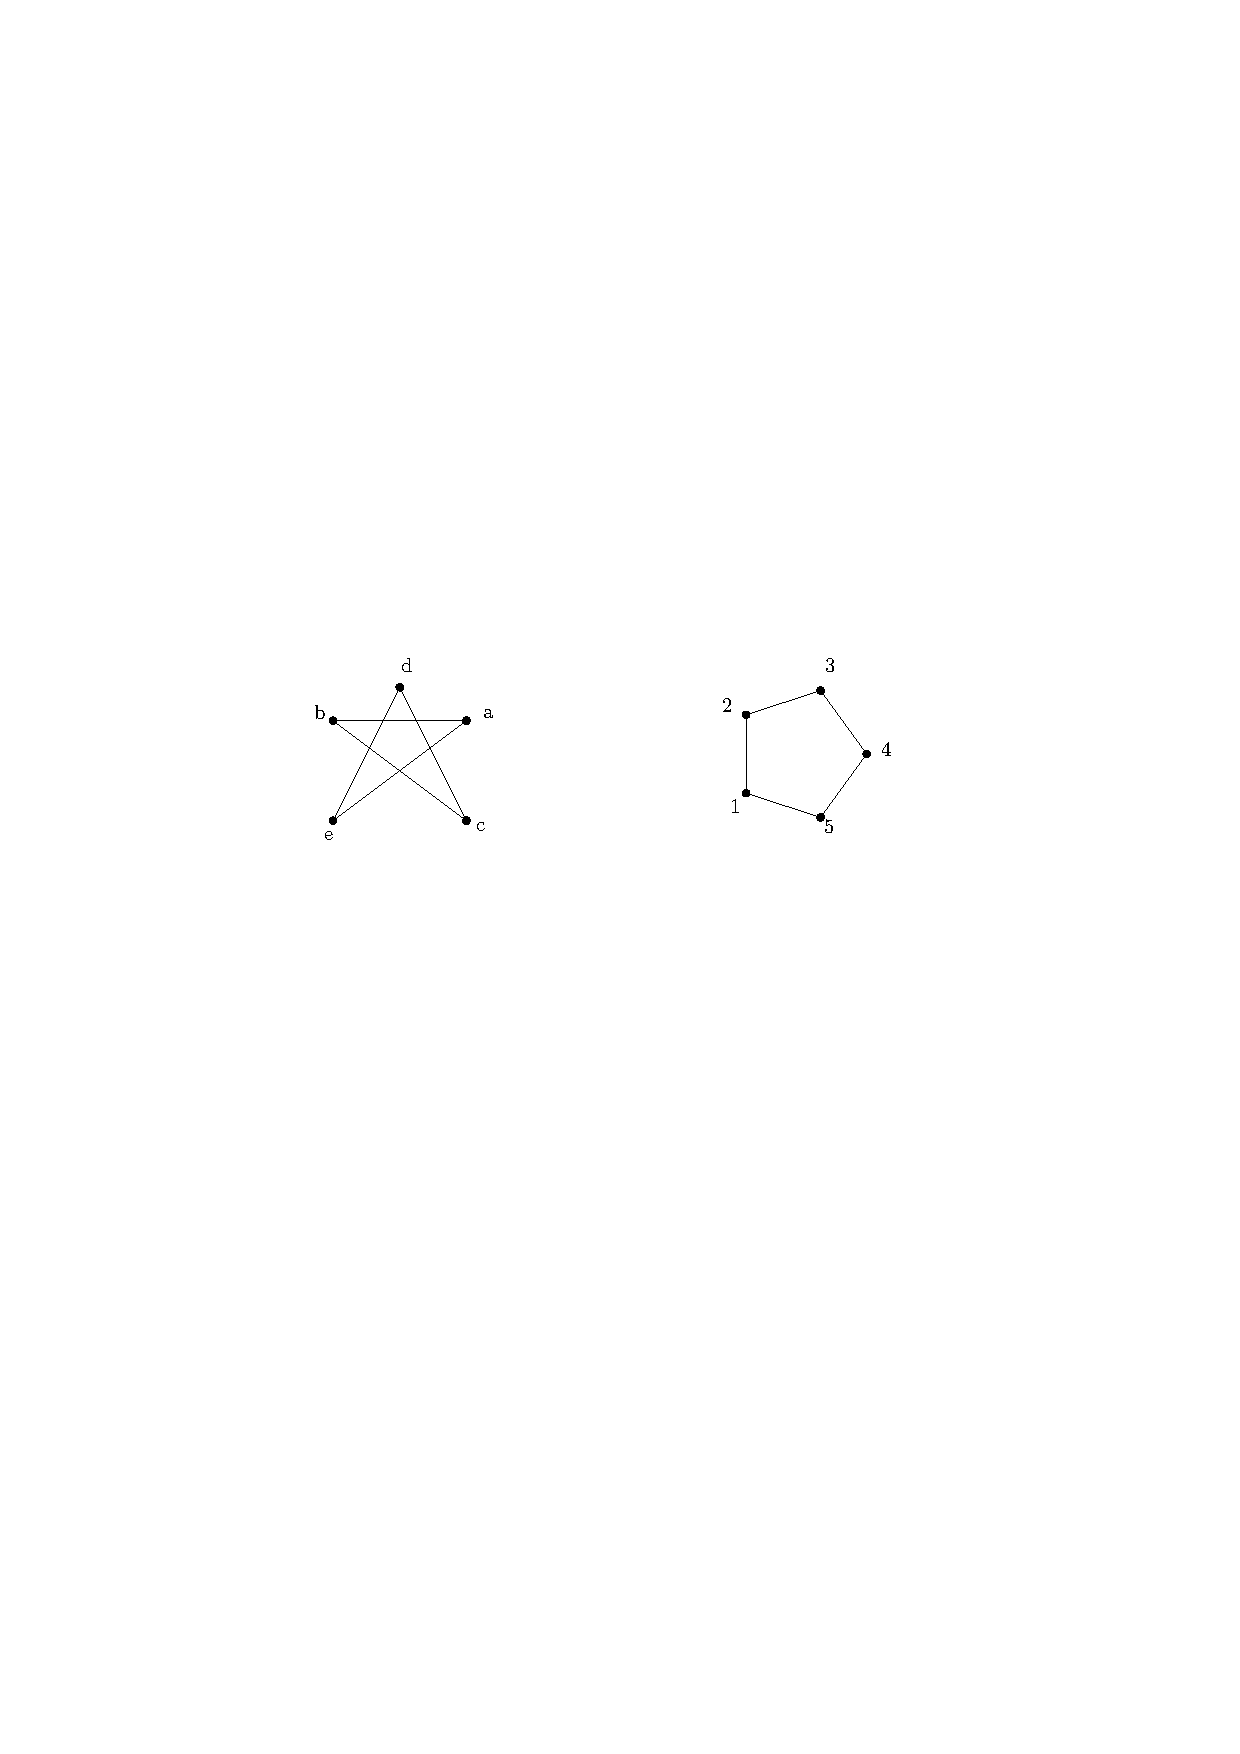
\includegraphics[scale=1]{graphics/graphIsomorphismExample.pdf}
\end{center} 
\caption{This figure depicts the graph isomorphism shown in Table \ref{table:ch1-graph-1} between $V_1$ and $V_2$.}
\label{fig:configuration-3}
\end{figure}

To visualize a graph, $G$, we create a drawing $\Gamma$, of $G$.  
The \textit{drawing} of a graph $G=(V,E)$ is an injective mapping $\Pi : V \mapsto \bbR^{2}$ which maps vertices to distinct points in the plane and for each edge $\curlybraces{u,v} \in E$, a continuous, injective mapping $c_{u,v}:[0,1]\mapsto \bbR^2$ such that $c_{u,v}(0) = \Pi(u)$, $c_{u,v}(1) = \Pi(v)$ , and the curve $c_{u,v}$ does not pass through any other vertex in $V$.
In this thesis, we will work with straight line drawings and orthogonal drawings.
Straight line drawings have mappings $c_{u,v}$ that are straight line segments.
Orthogonal drawings have mappings $c_{u,v}$ which are a sequence of alternating horizontal line segments and vertical line segments.
For orthogonal drawings, the endpoint of one line segment is the starting point of the next line segment, i.e. every $c_{u,v}$ is piecewise continuous.
The endpoints of the line segments of $c_{u,v}$ that are not $\Pi(u)$ or $\Pi(v)$ are called $\textit{bends}$.

\begin{figure}[!htbp]
\begin{center}
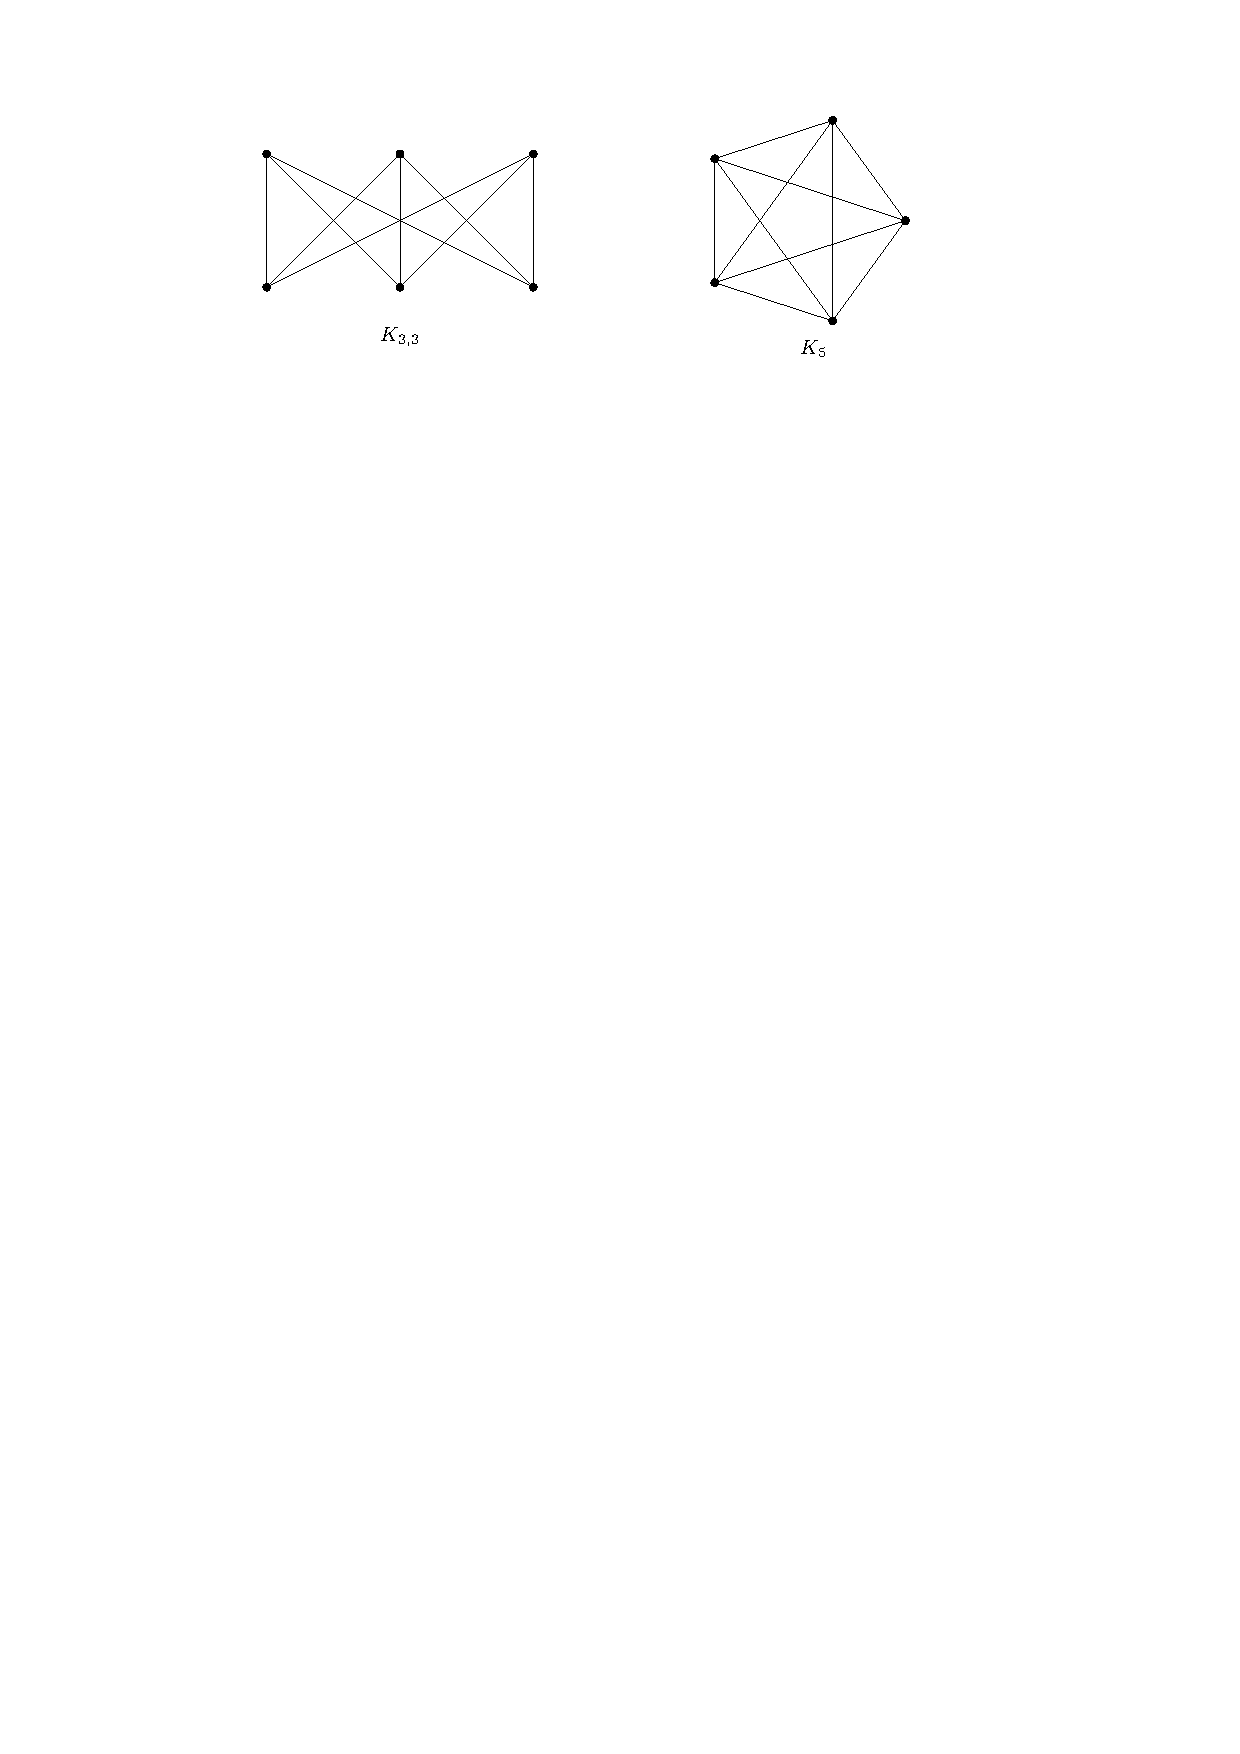
\includegraphics{graphics/kuratowskiExamples.pdf}
\caption{The $K_5$ and $K_{3,3}$ drawn in the plane.}\label{fig:kuratowskiExamples.pdf}
\end{center} 
\end{figure} 
Kuratowski's theorem characterizes finite planar graphs.
A finite graph is planar if and only if it does not contain a subgraph that is a subdivision of $K_5$ or $K_{3,3}$ \cite{kuratowski1930probleme}. 
Figure \ref{fig:kuratowskiExamples.pdf} shows a drawing of $K_5$ and $K_{3,3}$.
Two edges in a drawing \textit{cross} if they have a common interior point.  
The \textit{crossing number} of a graph is the smallest number of edge crossings for a graph over all drawings.
A drawing is said to be \textit{planar} if no two distinct edges cross \cite{BET+99}.
A planar drawing is also called an \textit{embedding}.
Two embeddings of a graph $G$ are \textit{equivalent} if for every vertex the counter-clockwise order of neighbors are the same.% determine the same circular order of the in neighbor sets and the embeddings can be described as a combination of translations and rotations of the other.
A combinatorial \textit{embedding} is a planar drawing with a corresponding counter-clockwise order of the neighbors of each vertex. 
\begin{figure}[!htbp]
\begin{center}
    \includegraphics{graphics/combinatorialEmbedding.pdf}
    \caption{Here is a wheel graph, $W_5$, in two separate drawings with the same counterclockwise ordering of neighbors for each vertex.}\label{fig:combinatorialEmbedding.pdf}
\end{center}
\end{figure}
An orientation preserving rigid transformation (i.e., rotation and translation) map an embedding to an equivalent embedding.  
Reflections reverse the counter-clockwise order around each vertex.

Figure \ref{fig:combinatorialEmbedding.pdf} depicts two different drawings of the wheel graph $W_5$.%, one on the left and one on the right. 
The drawings have the followings counterclockwise order of neighbors for each vertex:
\begin{table}[!htbp]\label{table:combinatorialEmbedding}
\begin{center}
$$\begin{array}{|c|c|c|}\hline
\text{Vertex}&\text{Left \& Middle Drawing}&\text{Right Drawing}\\\hline
1&(2,5,4)& (4,5,2) 
\\\hline
2&(3,5,1) & (1,5,3) 
\\\hline
3&(2,4,5)& (5,4,2) 
\\\hline
4& (1,5,3)  & (3,5,1) 
\\\hline
5&(2,3,4,1)& (4,3,2,1) 
\\\hline
\end{array} $$
\caption{A table showing the counter-clockwise circular ordering of neighbors for the left and right drawing in Figure \ref{fig:combinatorialEmbedding.pdf}.  Note that the permutation cycles are equivalent for the right and left drawings.}
\end{center} 
\end{table}
%The crossing number $cr\lr{\Gamma_G}$ of a drawing of $G$ is the number of crossings in the drawing of the graph $G$. 
%We can treat $cr()$ as a mapping from the space of drawings of $G$ to the non-negative integers, i.e. $cr: \left\lbrace \Gamma_G \right\rbrace \mapsto \bbZ^+ \cup \left\lbrace 0 \right\rbrace$.
%One can ask if for any graph $G$, does there exists a drawing in which the crossing number is zero?
%Without loss of generality, this is a type of crossing number minimization problem, i.e.
%$$ \min_{\gamma \in \left\lbrace \Gamma_G \right\rbrace} cr(\gamma)$$
Referencing table \ref{table:combinatorialEmbedding} and Figure \ref{fig:combinatorialEmbedding.pdf}, we realize that the two drawings of $W_5$ are equivalent.  



%If no two distinct edges intersect in the drawing, the drawing is said to be \textit{planar}. 



 






%Two planar drawings are equivalent if they determine the same circular orderings of the neighbor sets.
%Every proper drawing can be augmented to an embedded plane graph 
%by inserting new vertices at the edge crossings, and subdividing the edges that pass
%through those vertices. So the equivalence of two drawings reduces to the equivalence of plane graphs.


% A graph \textit{embedding} of $G = (V,E)$ is an injective mapping $\Pi: V \mapsto \bbR^2$.  
% \begin{figure}[!htbp]
% \begin{center}
% 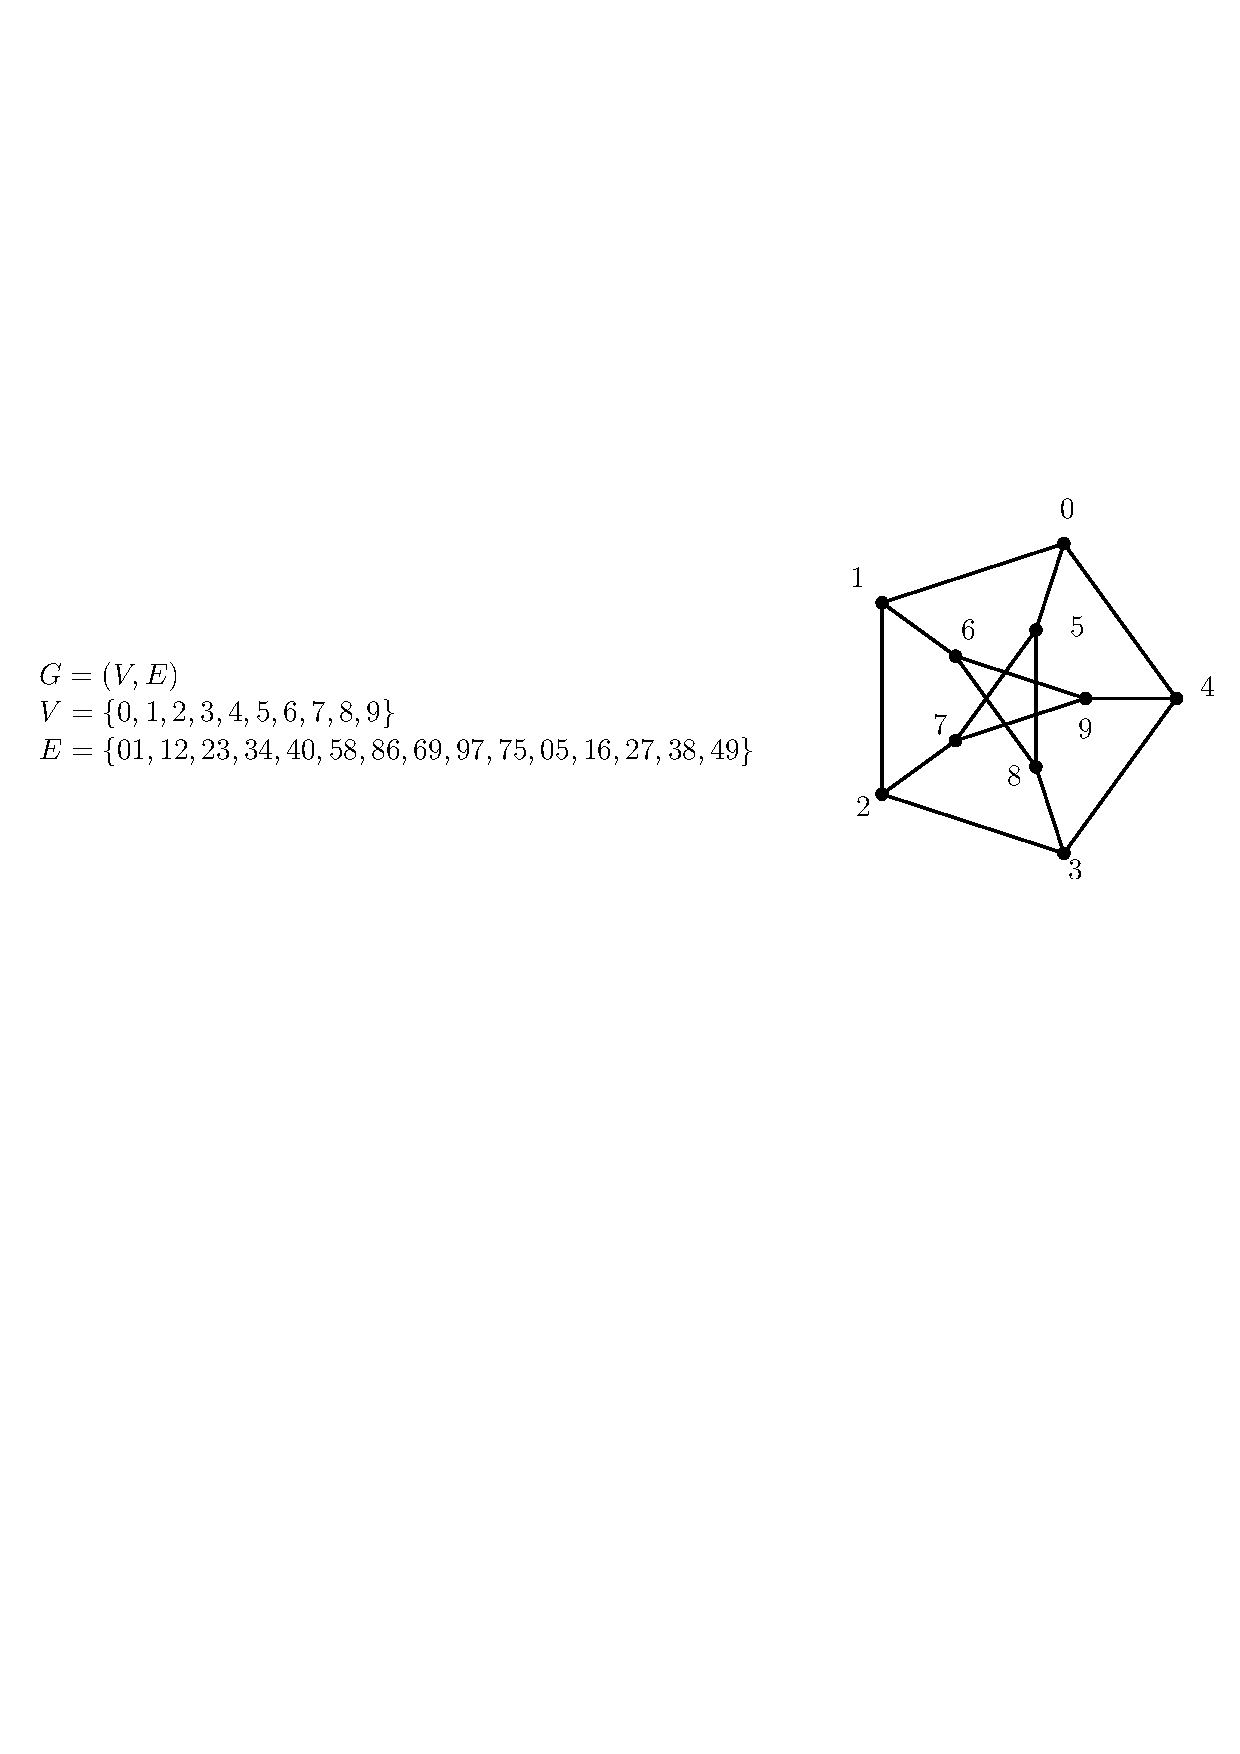
\includegraphics[scale=.5]{graphics/PetersonGraphExample.pdf}
% \caption{An embedding of the Peterson graph.}\label{fig:graph1-1}
% \end{center} 
% \end{figure} 
% A graph embedding is said to


% A \textit{graph} is an 
% ordered pair $G = (V,E)$ comprising of a set of vertices, $V$, and a set of edges or 
% lines, $E$.  Every edge $e \in E$, is an unordered pair of distinct vertices $u,v \in V$ (the edge represents their adjacency, $e = \{ u,v\}$). With this definition of a graph, there 
% are 
% no loops (self adjacent vertices, $\{v,v\}$) or multi-edges (several edges between the same pair of 
% vertices).

%   This requires an 
% embedding into the plane or $\bbr^3$.  An \textit{embedding} of the 
% graph $G = (V,E)$ is an injective mapping $\Pi : V \mapsto \bbR^{2}$ (see Figure 
% \ref{fig:graph1-1}). 


% \subsubsection{Edge Crossings}
% We define \textit{plane embeddings} of a graph to be an embedding where the following degenerate 
% configurations 
% do not occur:
% \begin{itemize}
% \item[\rn{1}] the interiors of two or more edges intersect, or
% \item[\rn{2}] an edge passes through a vertex
% \end{itemize} 
% \begin{figure}[H]
% \begin{center}
%   \begin{subfigure}[b]{0.49\textwidth}
% 	  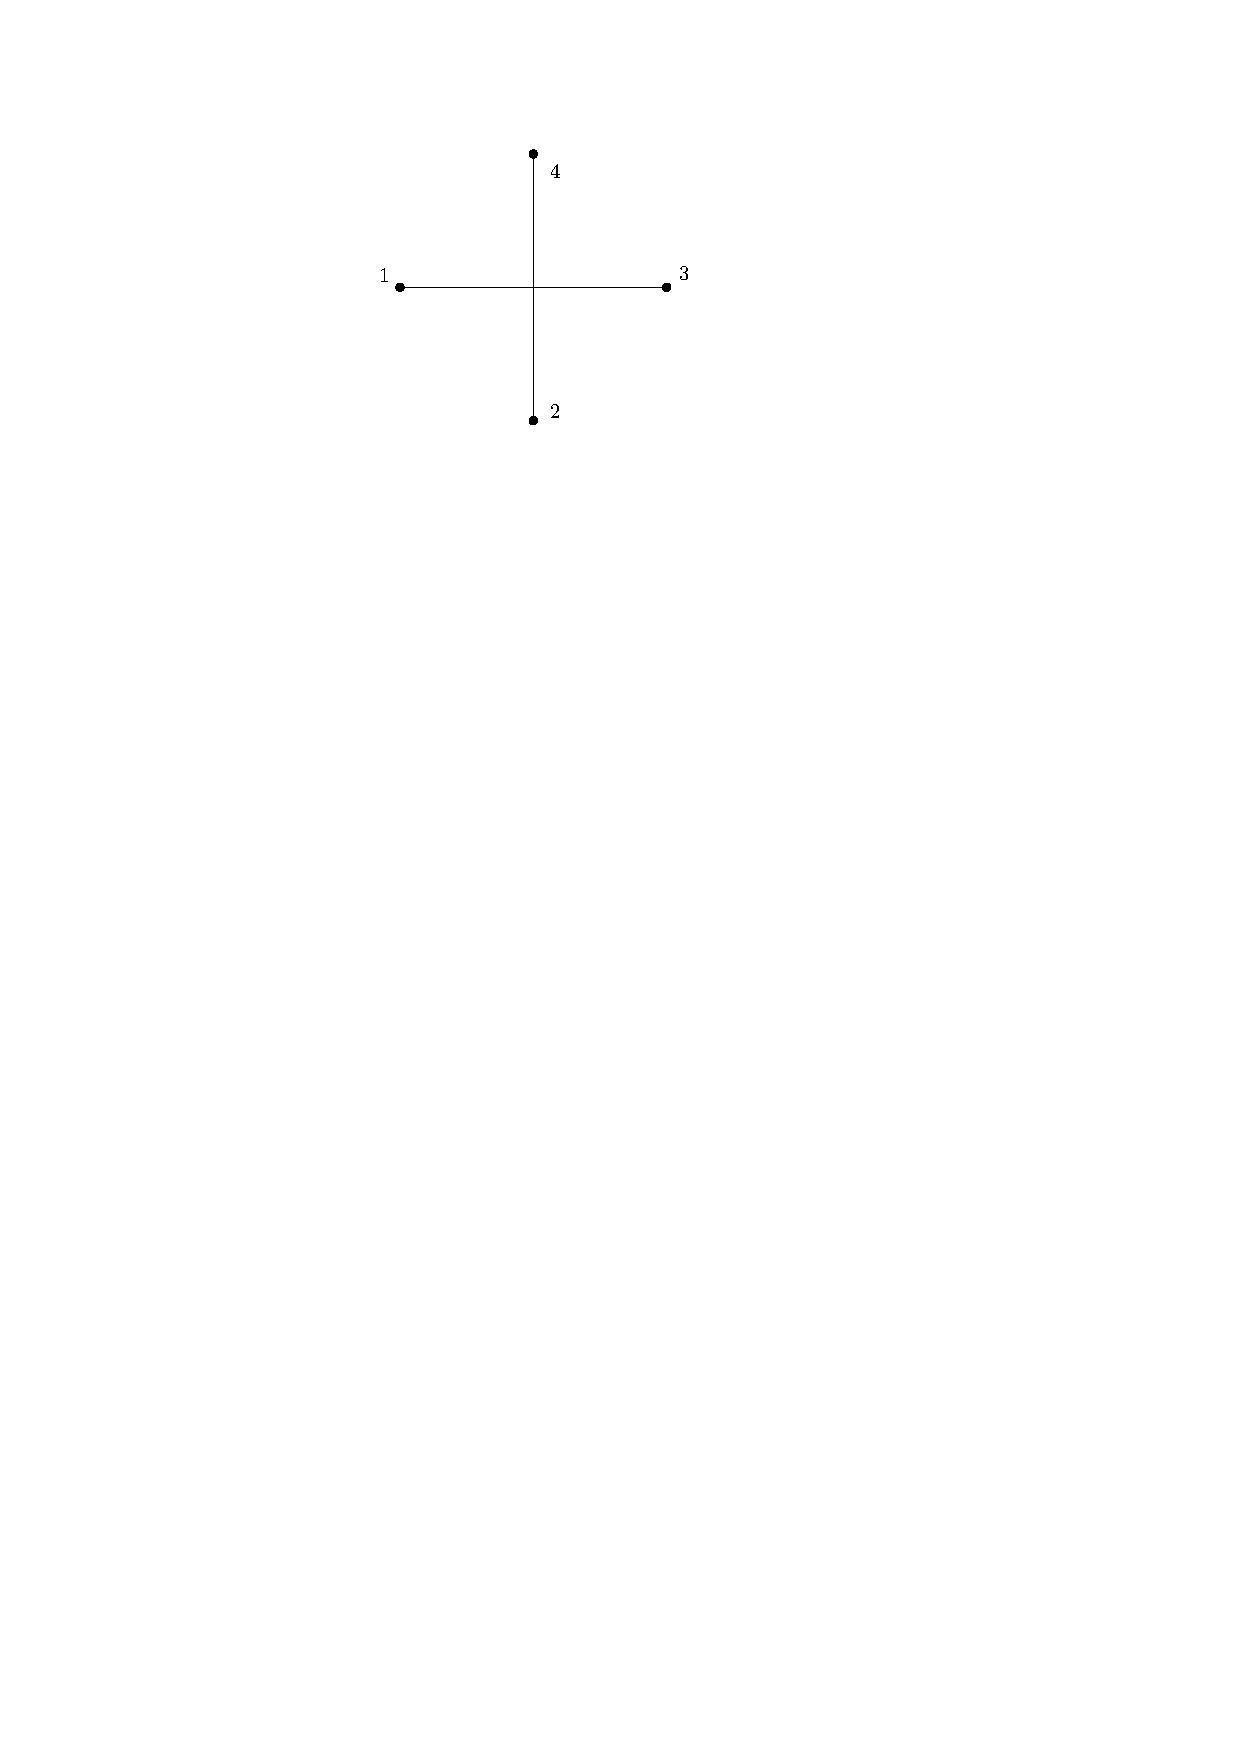
\includegraphics{graphics/crossingType2.pdf}
% 	  \caption{The interior of the edges intersect.}
% 	  \label{fig:ch1-linkages-1-2}
%   \end{subfigure}
%   \begin{subfigure}[b]{0.49\textwidth}
% 	  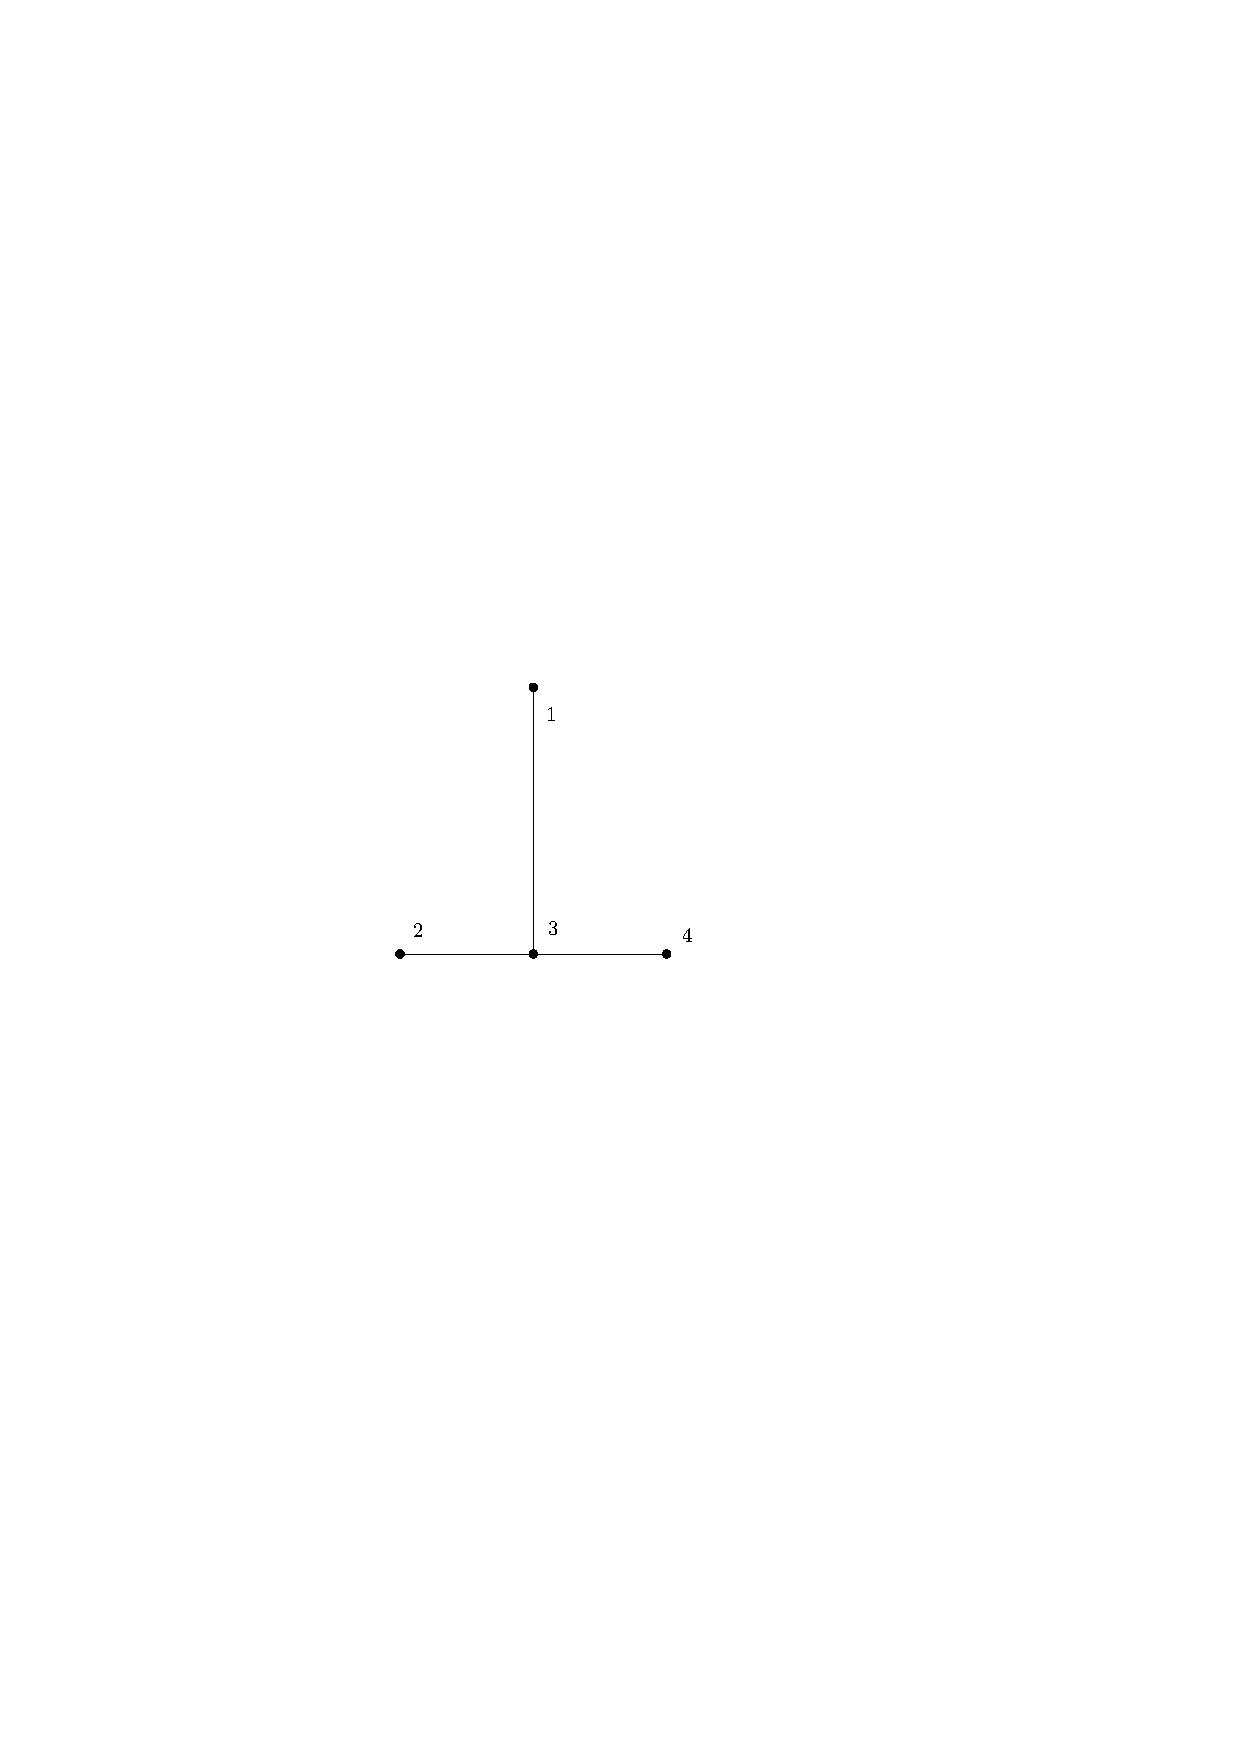
\includegraphics{graphics/crossingType3.pdf}
% 	  \caption{An edge passes through a vertex.}
% 	  \label{fig:ch1-linkages-1-3}
%   \end{subfigure}
% \end{center} 
% \caption{These figures exhibit the 4 types of edge crossings.}\label{fig:ch1-linkages-1}
% \end{figure}
% A graph is called \textit{planar} if it admits a plane embedding.  A \textit{plane graph} is a 
% graph together with a plane embedding.

\subsection{Trees}
%Some graphs can be classified by which properties they have.
A \textit{path} is a sequence of vertices in which every two consecutive vertices are connected by an edge.   
%\begin{figure}[!htbp]
\noindent%
\begin{minipage}{\linewidth}
\begin{center}
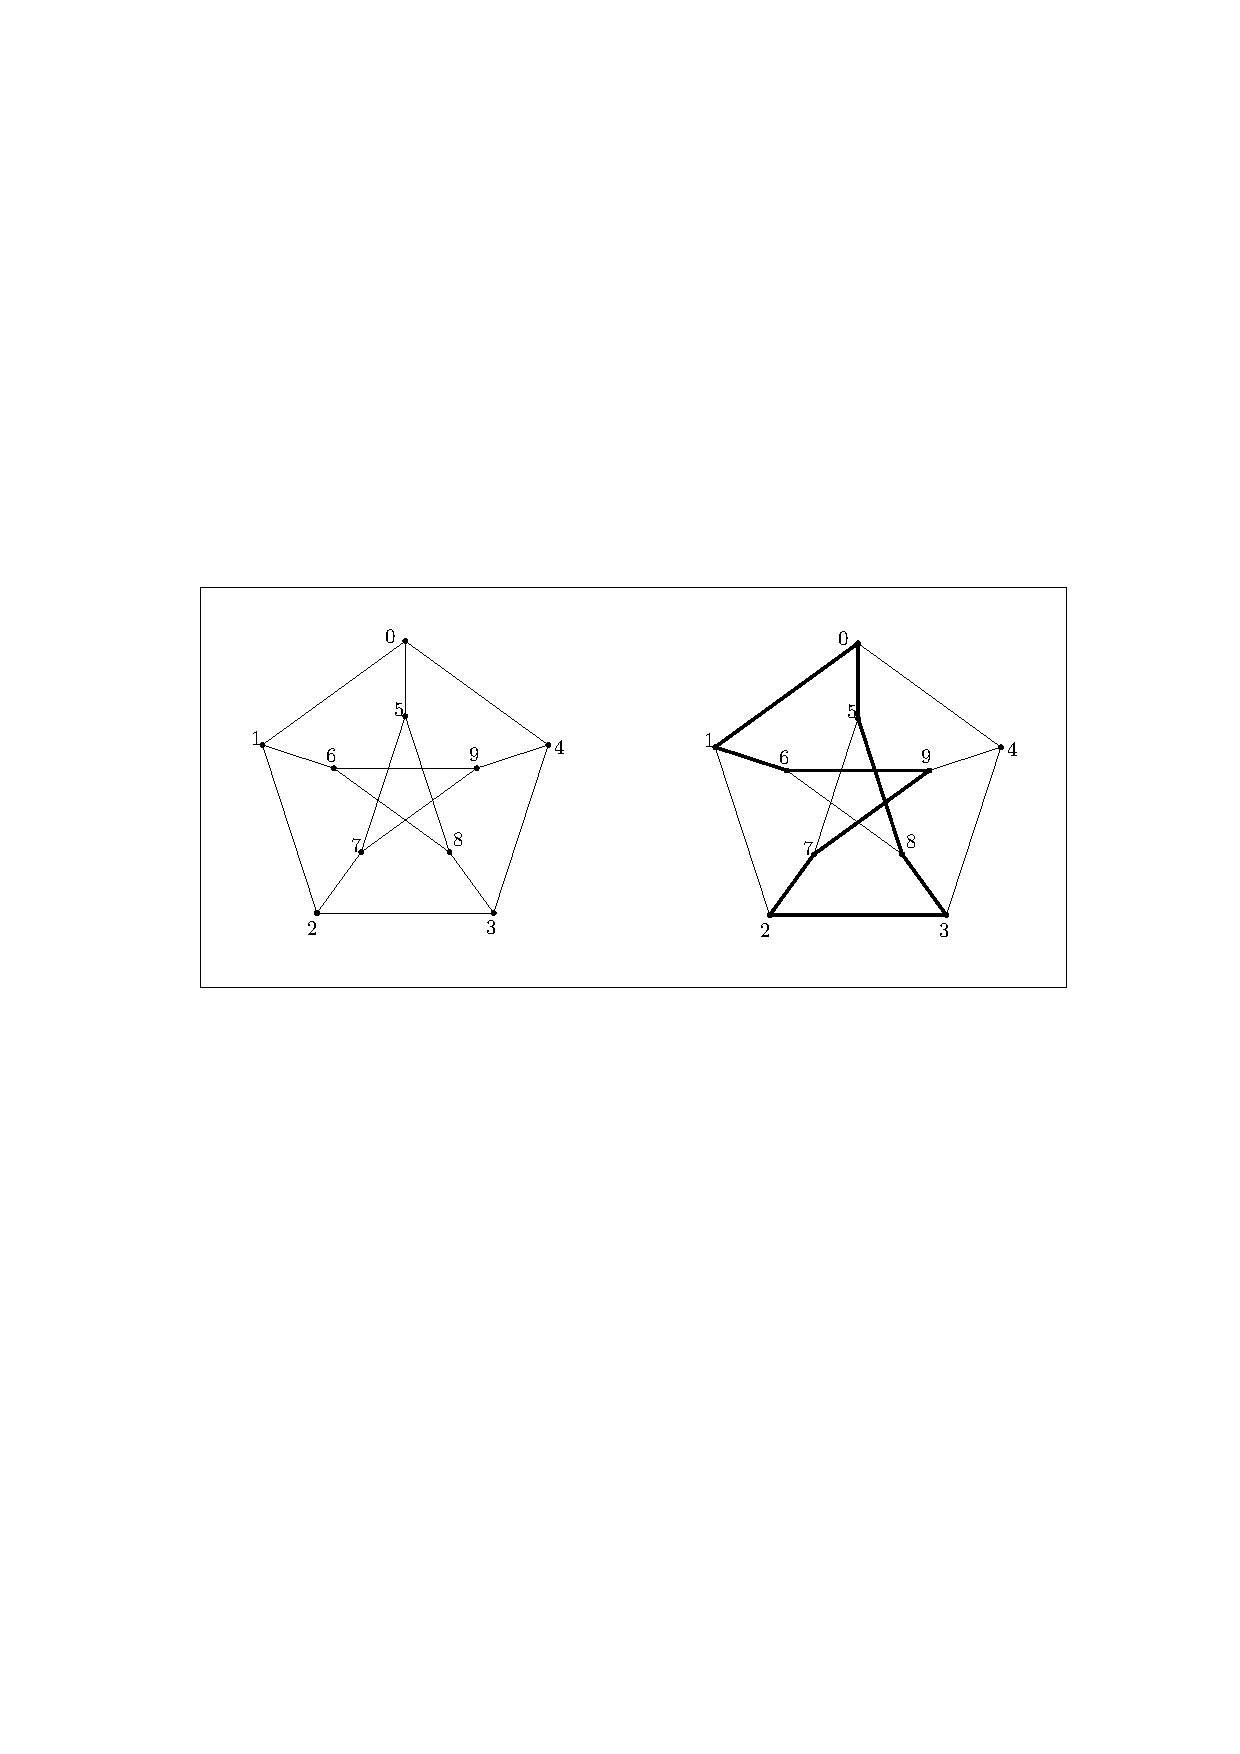
\includegraphics{graphics/PetersonGraphWithPath.pdf}
\captionof{figure}{An embedding of the Peterson graph with a simple cycle of 
(2,7,9,6,1,0,5,8,3).}\label{fig:PetersonGraphWithPath}
\end{center}
%\end{figure}
\end{minipage}
A \textit{simple cycle} of a graph is a sequence, $(v_1, v_2, \dots, v_{t-1},v_t)$, of distinct vertices such that every two consecutive vertices are connected by an edge,  and the last vertex, $v_t$, connects to $v_1$ (see Figure \ref{fig:PetersonGraphWithPath}).  
A graph is \textit{connected} if for any two vertices, there exists a path between the two points.
A \textit{tree} is a graph that has no simple cycles and is connected (see Figure \ref{fig:ch1-graph-2}).
Every tree is planar.
A \textit{forest} is a disjoint union of trees.  
%\begin{figure}[!hbpt]
\noindent%
\begin{minipage}{\linewidth}
\begin{center}
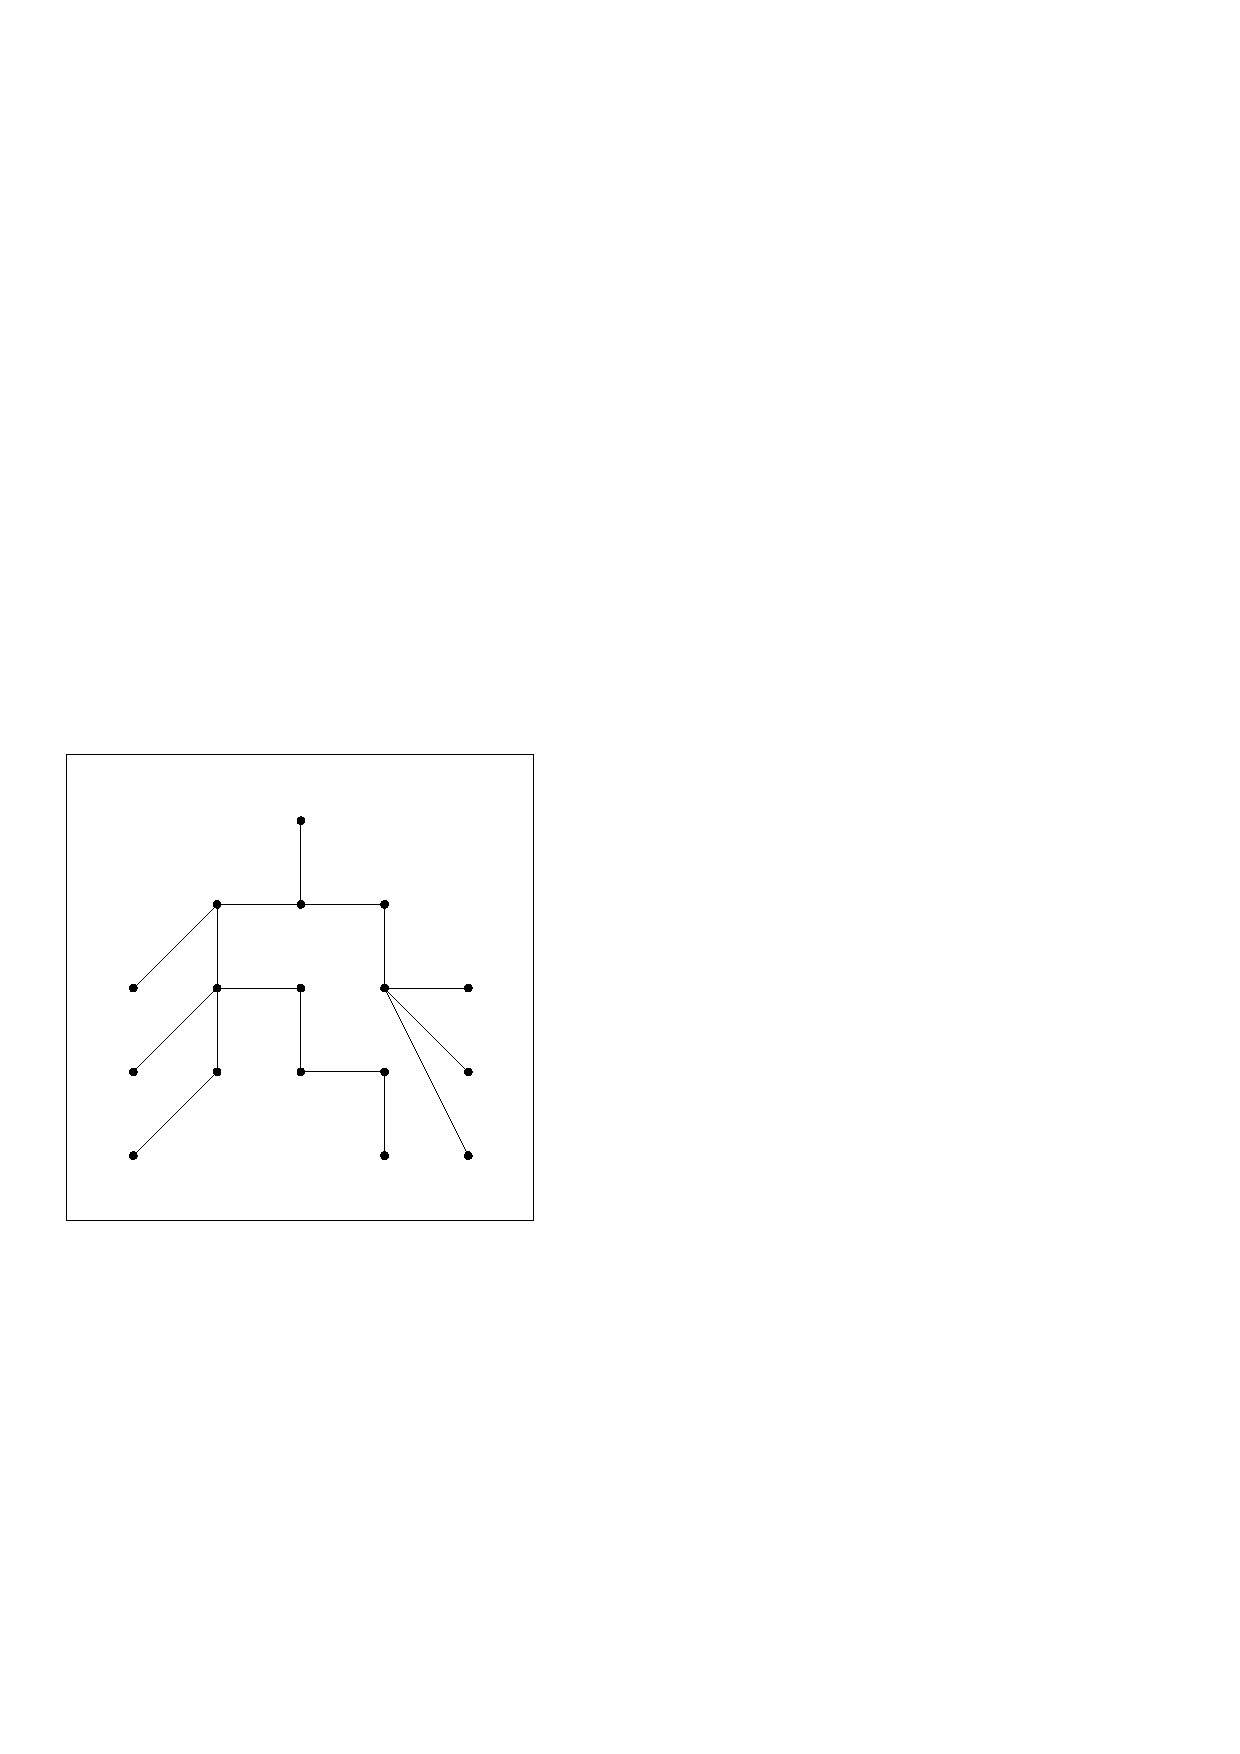
\includegraphics{graphics/RandomTree.pdf}
\captionof{figure}{An example of a tree.}\label{fig:ch1-graph-2}
\end{center}
%\end{figure}
\end{minipage}
%Any two embeddings of trees are equivalent if they can be described as any combination of rotations, translations, and or reflections.

% \subsection{Ordered Trees}
An \textit{ordered tree} is a tree $T$ together with a cyclic order of the neighbors for each vertex (see Figure \ref{fig:ch1-graph-6}).
%\begin{figure}[!hbpt]
\noindent%
\begin{minipage}{\linewidth}
\begin{center}
    \includegraphics{graphics/OrderedTreesExample.pdf}
    \captionof{figure}{A tree with two embeddings with different cyclic orderings around 
vertices.}\label{fig:ch1-graph-6}
\end{center}
%\end{figure}
\end{minipage}

Embeddings of ordered trees are combinatorially equivalent if for each node the counter-clockwise ordering of adjacent nodes are the same. 
%and can be described as a combination of translations and rotations of the other.
%Unlike embeddings for planar graphs where ordering of adjacent vertices is not a distinguishing condition,  we do not consider reflection based transformations for embeddings of ordered trees for equivaliency as that can modify the ordering of adjacent vertices.



% \subsection{Graph Isomorphism} 

% Next we add restrictions to our graph isomorphisms to narrow our focus:
% \begin{itemize}
% \item[\rn{1}] We focus on isomorphisms for planar graphs and or polygonal linkages, simple planar 
% graphs, and
% \item[\rn{2}] the isomorphism preserves edge lengths (polygonal area), e.g. $d(u,v) = d(f(u),f(v))$.
% \end{itemize}  
% With these restrictions of our isomorphisms, we can begin to describe a range of motion to 
% transform a linkage.  That range of motion is said to be the configuration space of that linkage.  
% To expand on this concept, for given linkage, $L=(V,E)$, and for a given vertex $v \in V$, the set 
% of points in which $v$ can be realized in the plane would be the configuration space for that 
% vertex, $C_v$.  Defining some order of the vertices in $L$, i.e. $V = \left\lbrace v_n 
% \right\rbrace_{i=1}^n$, then the \it{configuration space} for $L$ is said to be the cartesion 
% product of the configuration space of vertices:
% \subsection{Summary}
% \begin{table}[!ht]
% \begin{center}
% $$\begin{array}{|l|c|c|}
%  \hline
% &\text{Linkages}&\text{Polygonal Linkages}\\\hline
% \text{Ordered Pair}&G&G\\\hline
% \text{Edges}&E&\HH\\\hline
% \text{Vertices}&V&\PP\\\hline
% l&l&\text{N.A.}\\\hline
% \text{Embedding of }G&\Pi : V \mapsto \bbr^2&\PP ' = \left\lbrace P_i ' 
% \right\rbrace_{i=1}^n\\\hline
% \text{Realization}&\text{See (a)}&\text{See (b)}\\\hline
% \end{array}
% \caption
% $$
% \caption{(a)The realization for a linkage is for any edge $(u,v) \in E$ such that $\left\vert 
% \Pi(u)-\Pi(v)\right\vert = l(u,v)$.(b)A \emph{realization} of a polygonal linkage is an 
% interior-disjoint placement of congruent copies of the polygons in $\PP$ such that the points 
% corresponding to each hinge are identified (Fig. \ref{fig:1}, left).(c).}
% \end{center} 
% \label{table:linkages-2}
% \end{table} 
% %1) 
% %DESCRIBE THE FOLLOWING:
% %1)CONFIGURATION SPACE AS A VECTOR SPACE OF DIMENSION 2^N WHERE EDGE LENGTH IS PRESERVED.
% %2)PINNING 1 VERTEX TO ORIGIN AND A NEIGHBOR, ADD MOTIVATION TO PREVENT ROTATION AND TRANSLATIONS.
% 
% % \begin{equation}\label{eqn:linkages-1}
% % C(L) = C_{v_1} \cross C_{v_2} \cross \cdots \cross C_{v_n}
% % \end{equation} 
% % Some food for thought on configuration spaces and motions on linkages:
% % \begin{itemize}
% % \item[\rn{1}] A configuration space is said to be \it{connected} if there is a continuous mapping 
% for any two planar realizations (linkages) of a graph in the plane.  Otherwise it is said to be 
% \it{disconnected}.
% % \item[\rn{2}] If the configuration space of a vertex, $C_v$, is a singleton set, then the vertex 
% is said to be \it{pinned}. Otherwise it is said to be \it{free}.
% % \item[\rn{3}] The types of motions (mappings) that we refrain from using on linkages are 
% translations.
% % \end{itemize}
% % Note that configuration spaces for polygonal linkages are described similarly.
% % \subsubsection{Realizability of Linkages}
% % Suppose we had two configurations of a linkage, $\mathcal{A}$ and $\mathcal{B}$.  A question that 
% can be posed is can we reconfigure $\mathcal{A}$ to $\mathcal{B}$ continuously while respecting 
% simple planar graph conditions?  The answer to this question is a yes or no.  If yes, then there 
% must exist a path connected configuration space between $\mathcal{A}$ and $\mathcal{B}$.  It has 
% been shown that this problem can be posed as a planar satisfiability problem 
% \cite{Breu19983,mulzer2008minimum} (Later on in this paper we'll cover satisfiability problems).  
% This is the type of problem that we face in this paper.  We will continue to explore this in a 
% different manner, with circle packings.
% \newpage 
\section{Linkages}
\begin{figure}[!htbp]
 \begin{center}\label{fig:turkey}
  \includegraphics{graphics/HumanTurkeyLinkage.pdf}
  \caption{Here are skeleton drawings of a human and a turkey.  When animating skeletons, one tends to make sure that the lengths of the skeleton segments are kept the same length throught the animation.  Otherwise, the animation may depart from what is ideally understood of skeletal motions.}
 \end{center} 
\end{figure}

When graph drawings model physical objects, other qualities about the graph can be contextualized in a geometric sense.  
Distance, angular relationships and other geometric qualities may be relevant.
In any drawing, edges have length, angles formed by adjacent edges, and so on.  
In this thesis we are interested in the inverse problem where we would like to embed a graph with specific geometric properties, for example, an embedding with specified edge lengths. 
This motivates the following definition.
A \textit{length assignment} of a graph $G=(V,E)$ is a function $\ell:E \mapsto \bbr^+$. 
If $\ell(e)$ is the length of an edge $e$, $\ell(e)$ must be strictly positive in a drawing, otherwise it may result in two distinct vertices with the same coordinates.
Similar to combinatorial embeddings which is an equivalence class of embeddings of the same counter-clockwise order of vertices, we can also define an equivalence class of drawings with the same length assignment.
A \textit{linkage} is a graph $G = (V,E)$ with a length assignment $\ell:E \mapsto \bbr^+$ (e.g., see Figure \ref{fig:turkey}).
%Length assignments can be thought of as a metric where $\ell(u,v) = \ell(v,u)>0$.
%Inser linkage here




% \begin{figure}[!h]
% \begin{center}
% 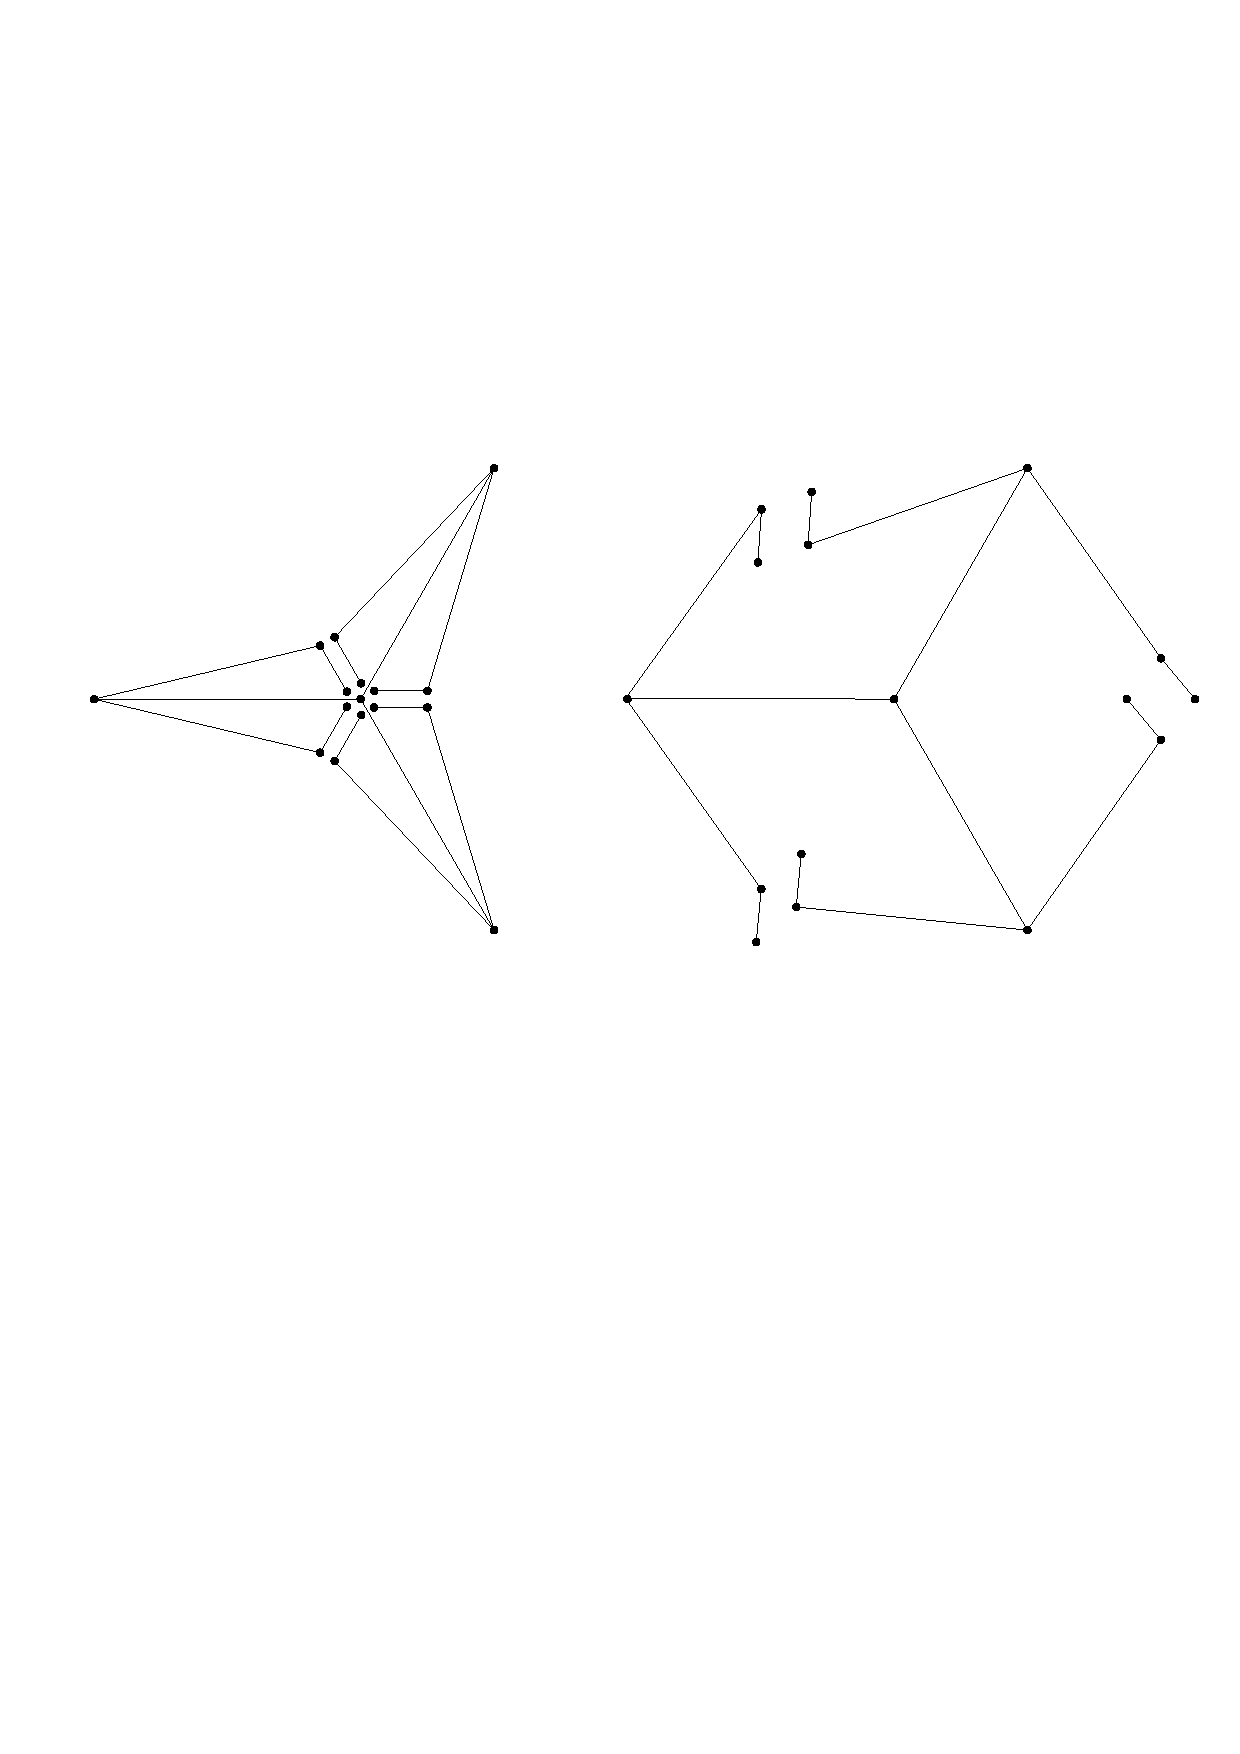
\includegraphics[scale=.75]{graphics/LockedConnellyLinkage.pdf}
% \end{center} 
% \caption{A linkage whose complete configuration space is discontinuous.  These two examples above 
% are two configurations of the same linkage that cannot continuously transform into the other 
% without edge crossing.}
% \label{fig:configuration-4}
% \end{figure}
% A \textit{reconfiguration} of a linkage whose graph is $G=(V,E)$ and length assignment is $\ell$ is 
% a continuous function $f: [0,1] \mapsto \bbr^{2 \cdot \vert V \vert}$ specifying a configuration of 
% the linkage for every $t \in [0,1]$ where length assignment $\ell$ is preserved, edges do not cross 
% and for every $\epsilon > 0$, there exists a $\delta > 0$ such that $\vert t_1 - t_2 \vert < 
% \delta$ implies 
% $$\left\vert f\left( t_1 \right) - f\left( t_2 \right) \right\vert < \epsilon$$

%(fig 1) insert a table of a graph and define a length assigment 
%(fig 2) insert a realization of (fig 1)
%(fig 3) insert a second realization of (fig 1)



%graph component of the linkage   the plane.  A linkage 
%\textit{embedding} is $L : V \mapsto 
%\bbR^{2}$.
% A \textit{linkage} is an ordered pair $G = (V,E)$ comprising of a set $V$ of vertices or nodes 
% together with a set $E$ of edges or lines. This definition is commonly used for graphs.  Mapping 
% the linkage $G$ into the plane is said to be the \textit{embedding}, i.e. $L : V \mapsto 
% \bbR^{2}$.  A length function correspond to a linkage, $l: E \mapsto \bbr^+$ gives a length to an 
% edge in the linkage.  If We consider a \textit{realization} of a linkage is range of $L$, i.e. 
% $L(V)$. If for every edge $(u,v) \in E$ such that $l\left( \left(u,v\right) \right) = \left\vert 
% L(u) - L(v) \right\vert$ is true, then $L$ is said to be a \textit{proper embedding} of $G$.
% \begin{figure}[h]
% \begin{center}
% 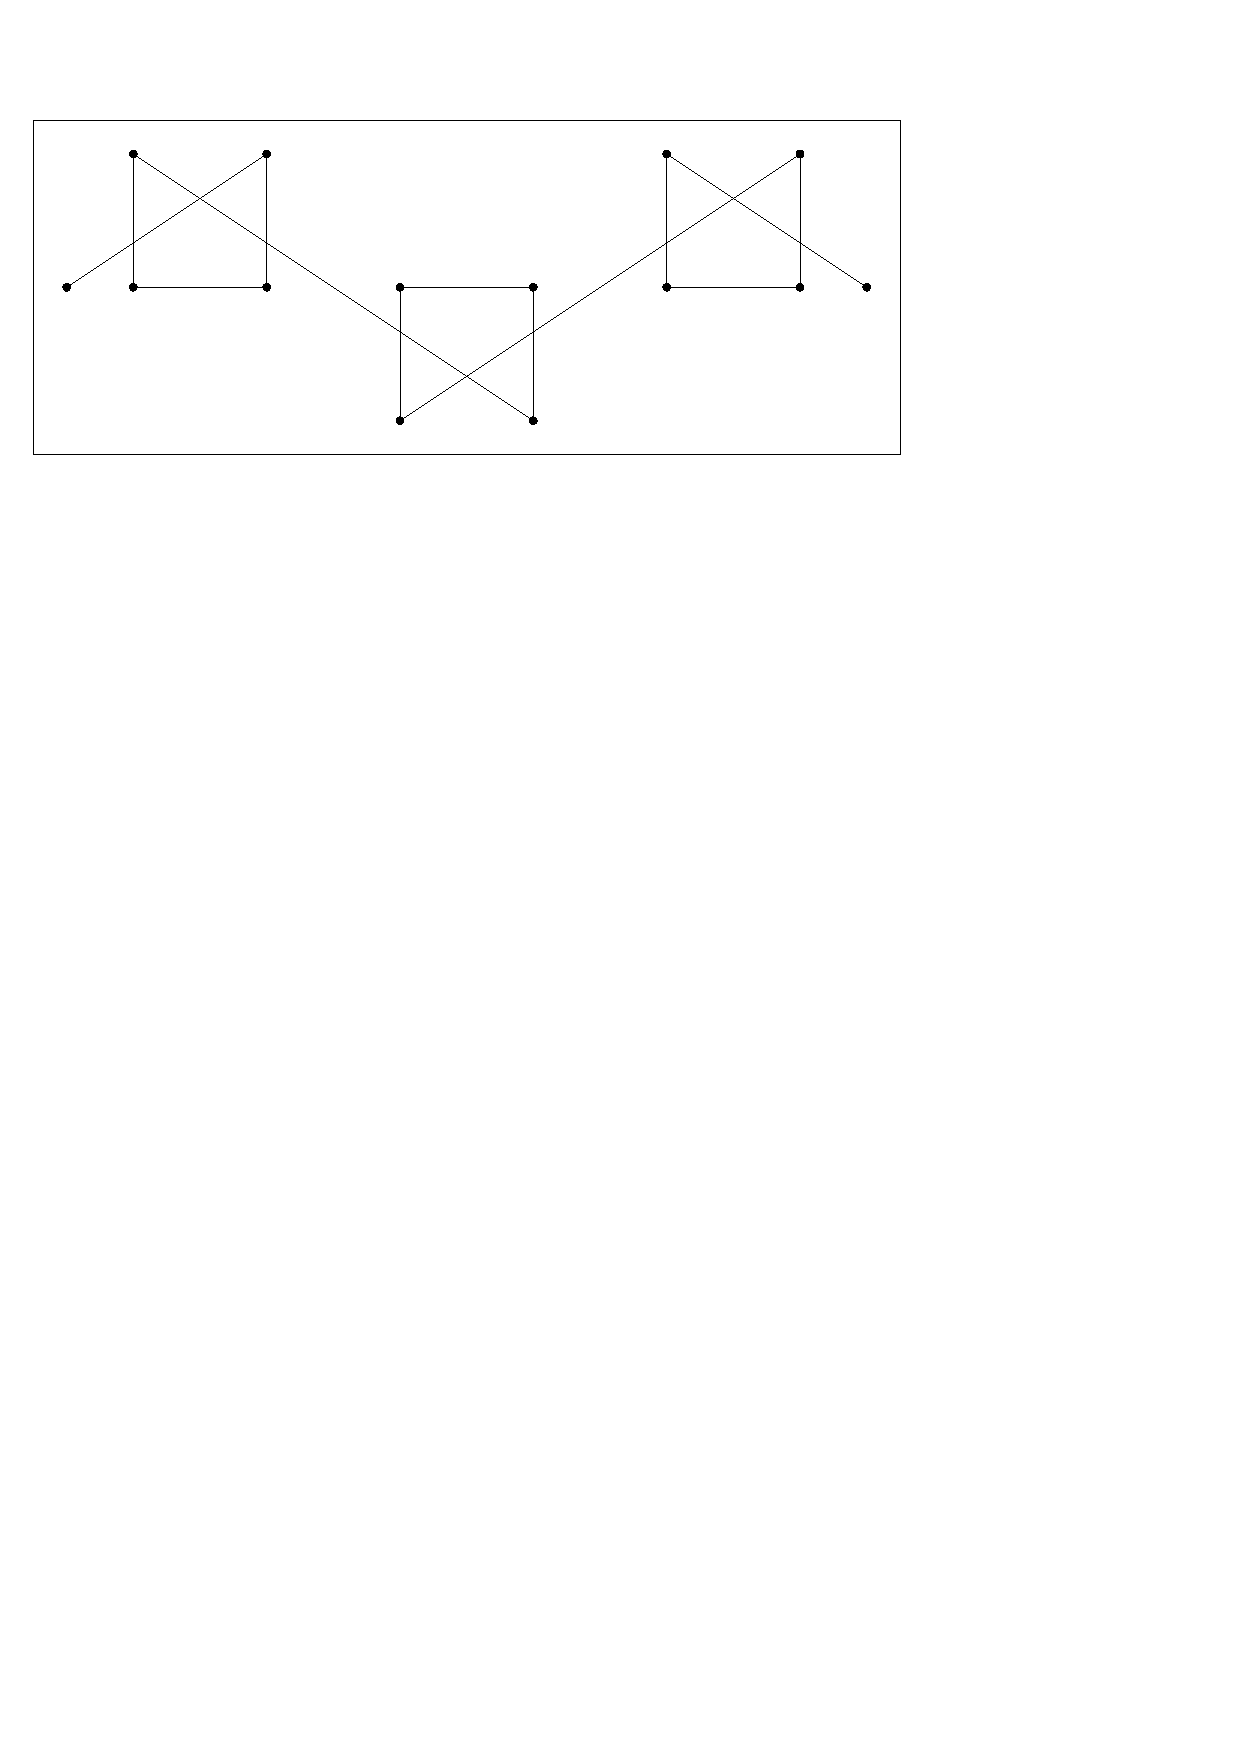
\includegraphics[scale=1]{graphics/crossingEdgeLinkage.pdf}
% \end{center} 
% \caption{A linkage where edges cross however it does not contain loops or multiple edges between 
% vertices.}
% \label{fig:linkage-3}
% \end{figure}
\section{Polygonal Linkages}
A generalization of linkages is a polygonal linkage where edges of given lengths are replaced with rigid polygons.
Formally, a \textit{polygonal linkage} is an ordered pair $\left(\PP,\HH \right)$ where $\PP$ is a finite set of polygons and $\HH$ is a finite set of hinges; a \textit{hinge} $h\in \HH$ corresponds to two or more points on the boundary of distinct polygons in $\PP$.  
A \emph{realization of a polygonal linkage} is an interior-disjoint placement of congruent copies of the polygons in $\PP$ such that the copies of a hinge are mapped to the same point (e.g., Figure \ref{fig:linkage-1}).  
\begin{figure}[!htbp]
\begin{center}
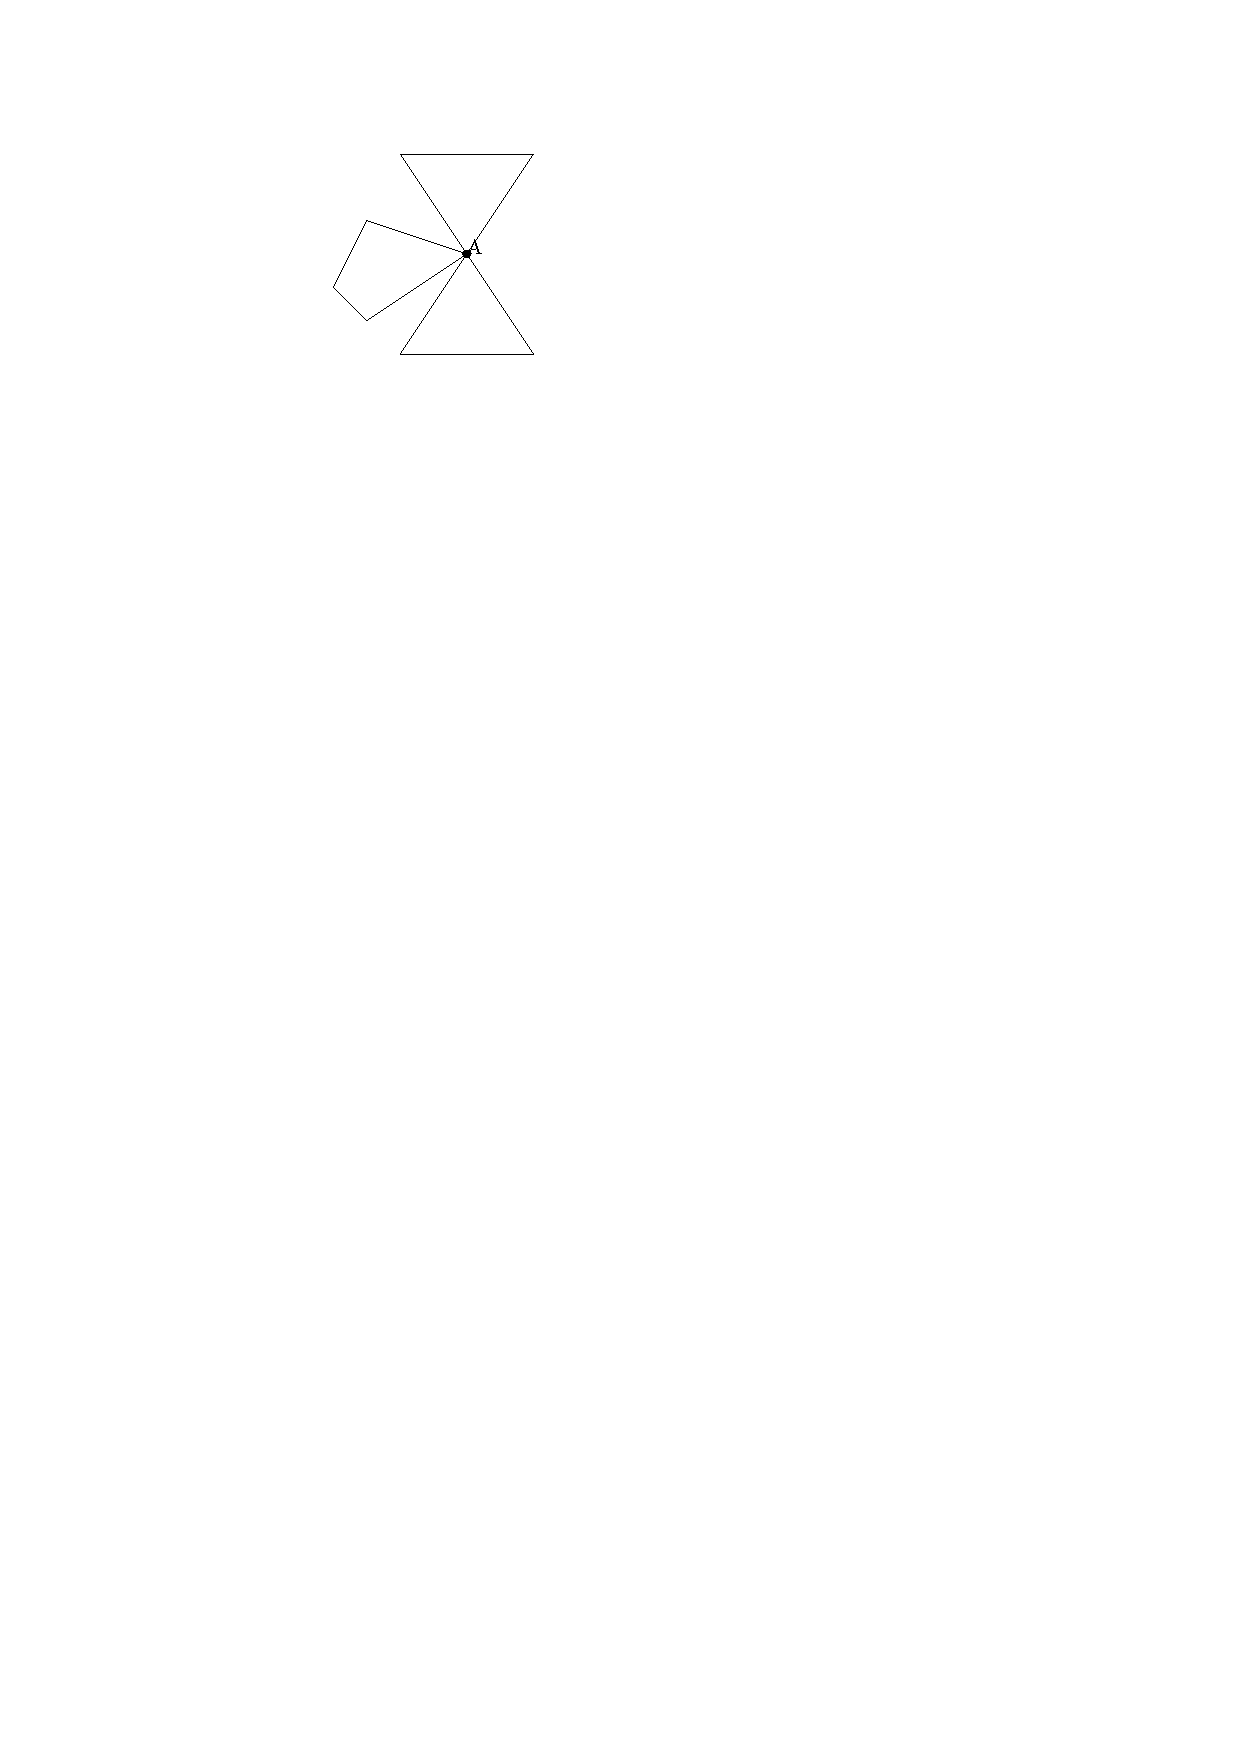
\includegraphics[scale=1]{graphics/hingeOnThreeDistinctPolygons.pdf}
\end{center} 
\caption{(a) A polygonal linkage with a non-convex polygon and two hinge points corresponding to 
three polygons.  Note that hinge points correspond to two distinct polygons.(b) Illustrating that 
two hinge points can correspond to the same boundary point of a polygon.}
\label{fig:linkage-1}
\end{figure}
A \textit{realization of a polygonal linkage with fixed orientation} is a realization in which each polygon is translated and rotated copy of a polygon in $\PP$; at each hinge the incident polygons are in a given counter-clockwise order (refer to Figure \ref{fig:orderedLinkages}).
%the congruent copies of the polygons in $\PP$ is translated and rotated copy in $\PP$.
% each copy allows for any combination of translations and rotated copies of polygons in $\PP$ where every hinge has a counter-clockwise order of incident polygons.  
\begin{figure}[!htbp]\label{fig:orderedLinkages}
\begin{center}
\includegraphics[scale=1]{graphics/orderedLinkages.pdf}
\end{center} 
\caption{Two realizations of the same polygonal linkage with that differ in the counter-clockwise order of polygons around vertex $a$. }
\end{figure}
Note that oriented polygonal linkage realizations do not allow for reflection transformations of polygons in $\PP$.

These two realization types allow one to pose two different problems, the realizability problem for polygonal linkages and the realizability problem for polygonal linkages with fixed orientation:
\begin{prob}[Realizibility Problem for Polygonal Linkages]\label{problem:UnorderedPolygonal}
%The realizability problem for a polygonal linkage asks whether a given polygonal linkage has 
%a realization.
Given a polygonal linkage, does it have a realization?
\end{prob}
\begin{prob}[ Realizibility Problem for Polygonal Linkages with Fixed Orientation]\label{problem:OrderedPolygonal}
%The \emph{realizability} problem for a ordered polygonal linkage asks whether a given polygonal 
%linkage has a realization with respect to order.
Given a polygonal linkage with fixed orientation, does it have a realization?
\end{prob}
%Refer to Figure \ref{fig:orderedLinkages} to a polygonal link
Not every polygonal linkage has a realization.
\begin{figure}[!htbp]
\begin{center}
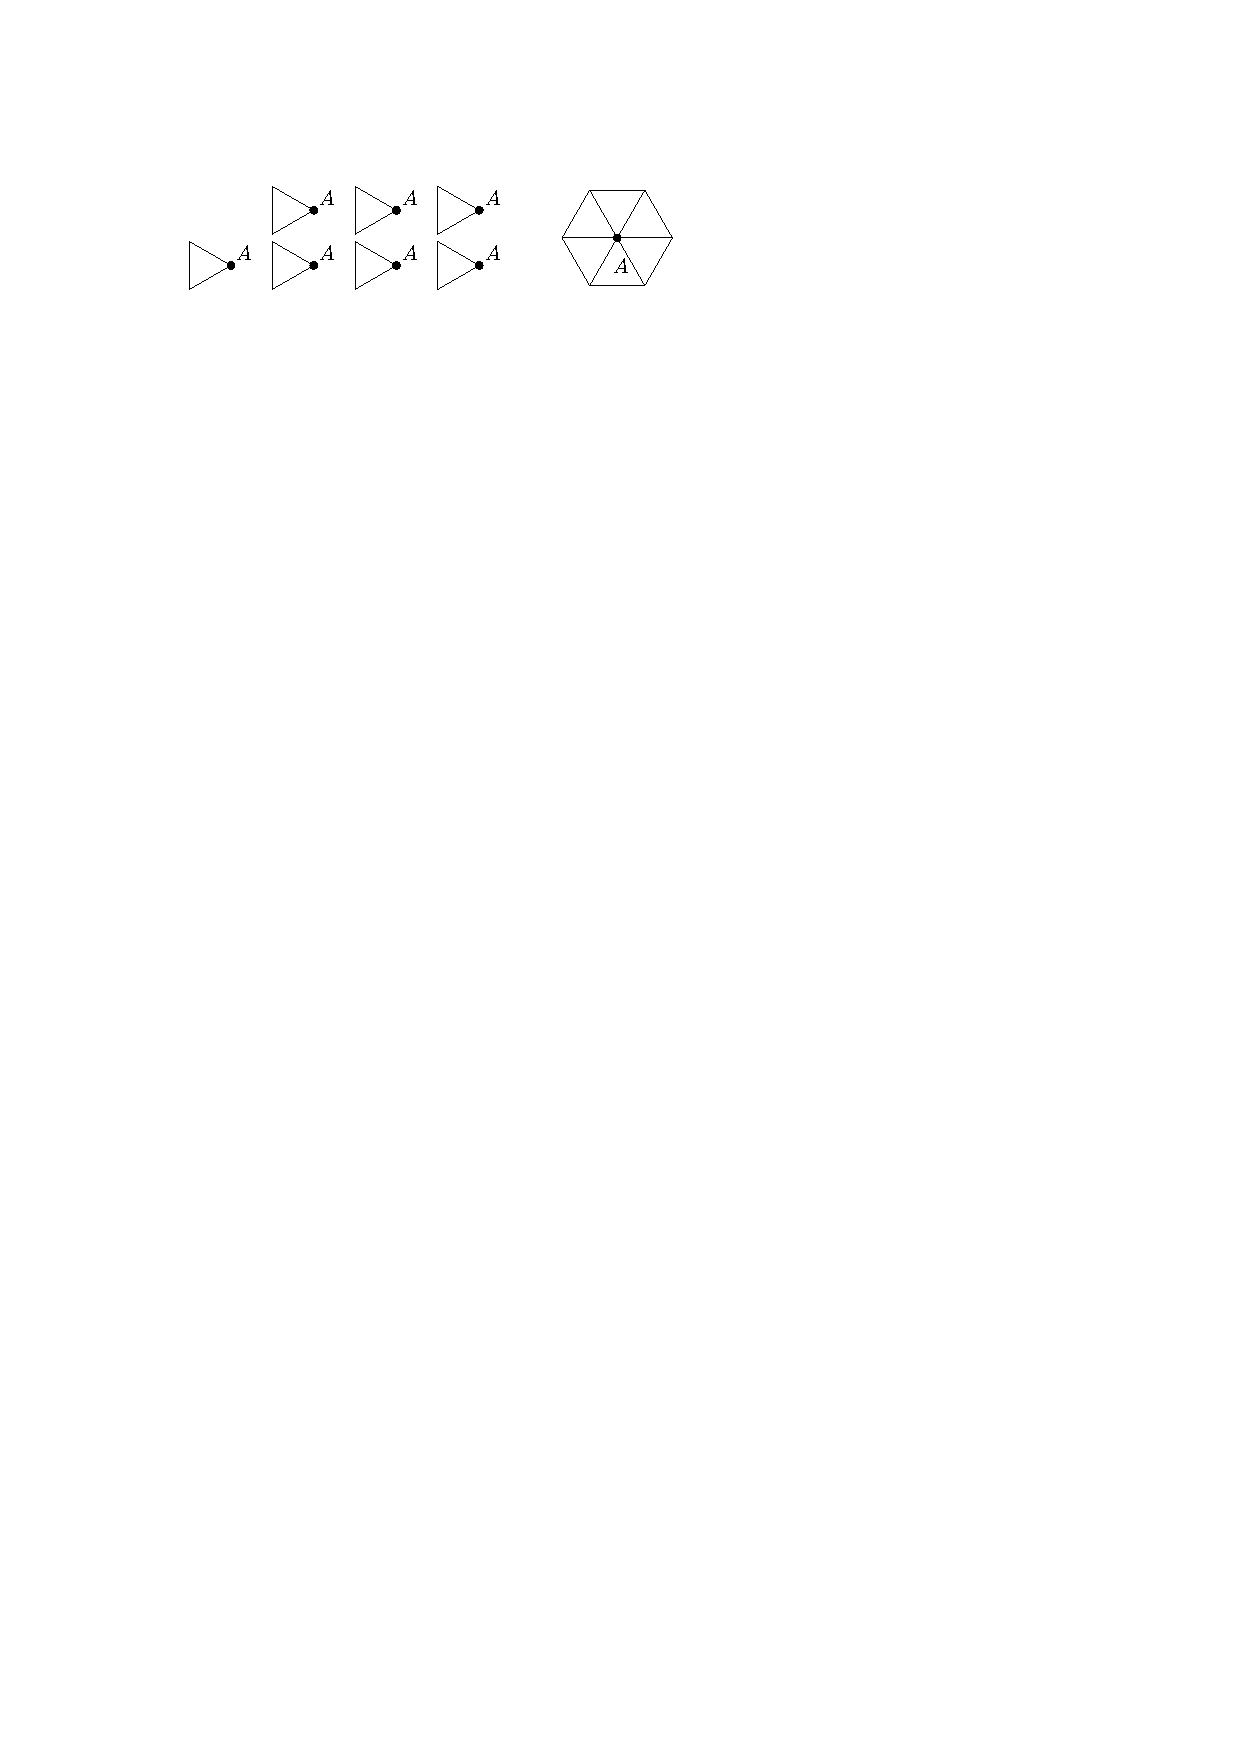
\includegraphics[scale=1]{graphics/Problem1.pdf}
\end{center} 
\caption{Here we have 7 congruent copies of an equilateral triangle with a hinge point of $A$.  The polygonal linkage is not realizable.  The best we can realize is at most 6 congruent copies of an equilateral triangle with the hinge point of $A$ in the plane.}
\label{fig:problem1}
\end{figure}
Consider the 7 congruent copies of an equilateral triange with a common hinge point in Figure \ref{fig:problem1}.
To show it does not have a realization, suppose it is realizable.  
Each angle of every triangle is $\frac{\pi}{3}$ radians.  
The sum of 7 angles formed by the triangles is $\frac{7\pi}{3}>2\pi$.  
The total radian measure around $A$ is $2 \pi$.
%In an interior disjoint placement of the triangles, the sum of angles incident at any point is at most $2\pi$.
The contradiction is that the sum of 7 angles formed by the triangles in an interior disjoint placement is $\frac{7\pi}{3}$.
%This exceeds the total radian measure around $A$ and so we cannot have a realization.
The polygonal linkage of Figure \ref{fig:problem1} would overlap itself and does not have a realization.

There are polygonal linkages that admit realizations but every realization requires rotation.
Figure \ref{fig:collidingHingedPolygons} show the congruent copies of the polygons $A$, $B$, $C$, and $D$ in two different configurations, the far right is a realization, the middle fails to be a realization because of the interiors of $B$ and $D$ intersecting and the left showing the polygons in $\PP$.  
In fact, this polygonal linkage cannot admit a realization with fixed orientation.
Indeed this polygonal linkage cannot satisfy Problem \ref{problem:OrderedPolygonal}, suppose there is a realization with fixed orientation.  
Without loss of generality, fix the placement of $C$.
$A$, $B$, and $D$ have unique placement around triangle $C$.  
In this placement $C$ and $D$ overlap.%have common intersecting interiors and thus a contradiction of the existence of a realization.  
\begin{figure}[!htbp]\label{fig:collidingHingedPolygons}
\begin{center}
\includegraphics[scale=1]{graphics/collidingHingedPolygons.pdf}
\end{center} 
\caption{This example shows yet another example where two realizations of the same polygonal linkage. 
 One realization where there is an intersection and another where there isn't an intersection.}
\end{figure}
Figure \ref{fig:collidingHingedPolygons}, satisfies Problem \ref{problem:UnorderedPolygonal} but not Problem \ref{problem:OrderedPolygonal}.
 The far right is a realization but with polygon $B$ reflected.
  %If $B$ were not reflected we see that the only way to attach the polygons by their hinges together is if $B$ and $D$ intersect in their interiors.  

Figure \ref{fig:collidingHingedPolygons} does not quite get at the heart of the challenge with Problem \ref{problem:UnorderedPolygonal} because the counter-clockwise order of the polygons around hinges is not considered.

\begin{minipage}{\linewidth}
\begin{center}
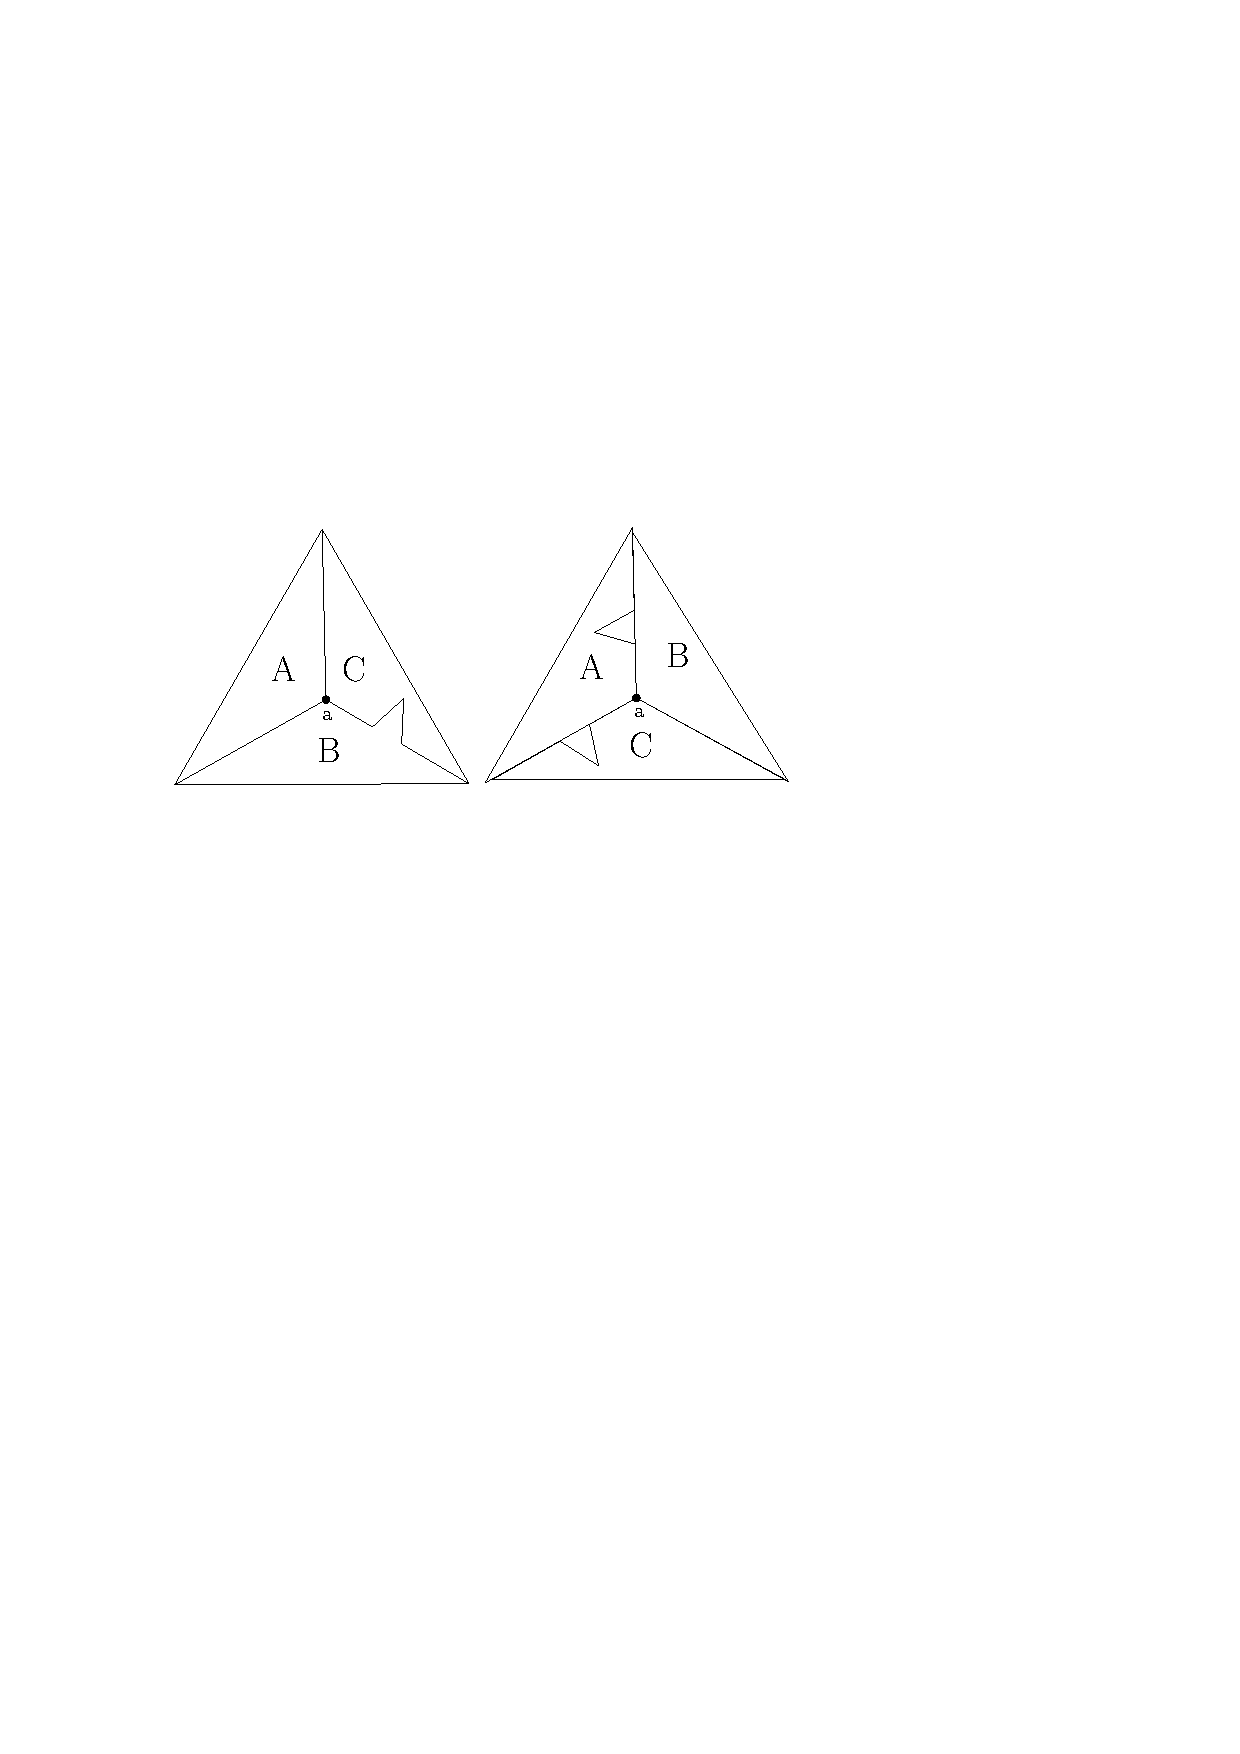
\includegraphics[width=.33\columnwidth]{graphics/orderedFaces.pdf}
\end{center}
\captionof{figure}{Here we have two realizations of a polygonal linkage with two different counter-clockwise order (C,B,A) and (B,C,A) respectively.  
Note that the placement with ordering (B,C,A) has an overlap.}\label{fig:orderedFaces.pdf}
\end{minipage}

Figure \ref{fig:orderedFaces.pdf} shows three polygons with a common hinge.
In the counter-clockwise order $(A,B,C)$, the polygonal linkage admits a realization whereas in the counter-clockwise order $(A,C,B)$, it does not admit a realization.
The examples above show that answers to Problem \ref{problem:UnorderedPolygonal} and \ref{problem:OrderedPolygonal} could be yes or no; the answer could be negative for various reasons.
Sections 2 and 3 of this thesis address the computational complexity of solving Problems \ref{problem:UnorderedPolygonal} and \ref{problem:OrderedPolygonal}.
We show that both problems are intractable.




\subsection{Geometric Dissections}
Hilbert's third problem asks: given any two polyhedra of equal volume, is it always possible to cut the first into finitely many polyhedral pieces which can be reassembled to yield the second \cite{aigner2010hilbert}?  
In three dimensions the answer is no however for two dimensions it is true \cite{10.23073621846}.

The Wallace-Bolyai-Gerwien Theorem simply states that two polygons are congruent by dissection iff they have the same area.  
A \textit{dissection} being a collection of smaller polygons whose interior disjoint union forms a polygon.
Hinged dissections of a polygon $P$ is a polygonal linkage that admits a realization that forms $P$.  
%The question of given two polygons of equal area, does there exist a hinged dissection whose two possible realizations are the polygons?
Demaine et. al. \cite{abbott2012hinged} showed that any two polygons of the same area have a common hinged dissection where polygonal pieces must hinge together at vertices to form a connected realization and that there exists a continuous motion between the two realizations (refer to section 1.5.3).
The was an outstanding problem for many years until 2007.

The Haberdasher Puzzle was proposed in 1902 by Henry Dudeney: can a square and an equilateral triangle of the same area have a common dissection into four pieces? 
%%%add story about the puzzle%%%%

\begin{minipage}{\linewidth}
\begin{center}
\includegraphics{graphics/HaberdasherProblem.pdf}
\end{center}
\captionof{figure}{The Haberdasher Puzzle was proposed in 1902 and solved in 1903 by Henry Dudeny.  The dissection is for polygons that forms a square and equilateral traingle.}
\label{fig:polygonallinkage-5}
\end{minipage}

Geometric dissections are closely related to polygonal linkages.  
Figure \ref{fig:polygonallinkage-4} shows two arrangements of the same polygons to form a hexagon and a square. 
The polygons are not hinged and are arranged in differing order.
The polygons are merely tiled together to form the hexagon and square. 

\begin{minipage}{\linewidth}\begin{center}
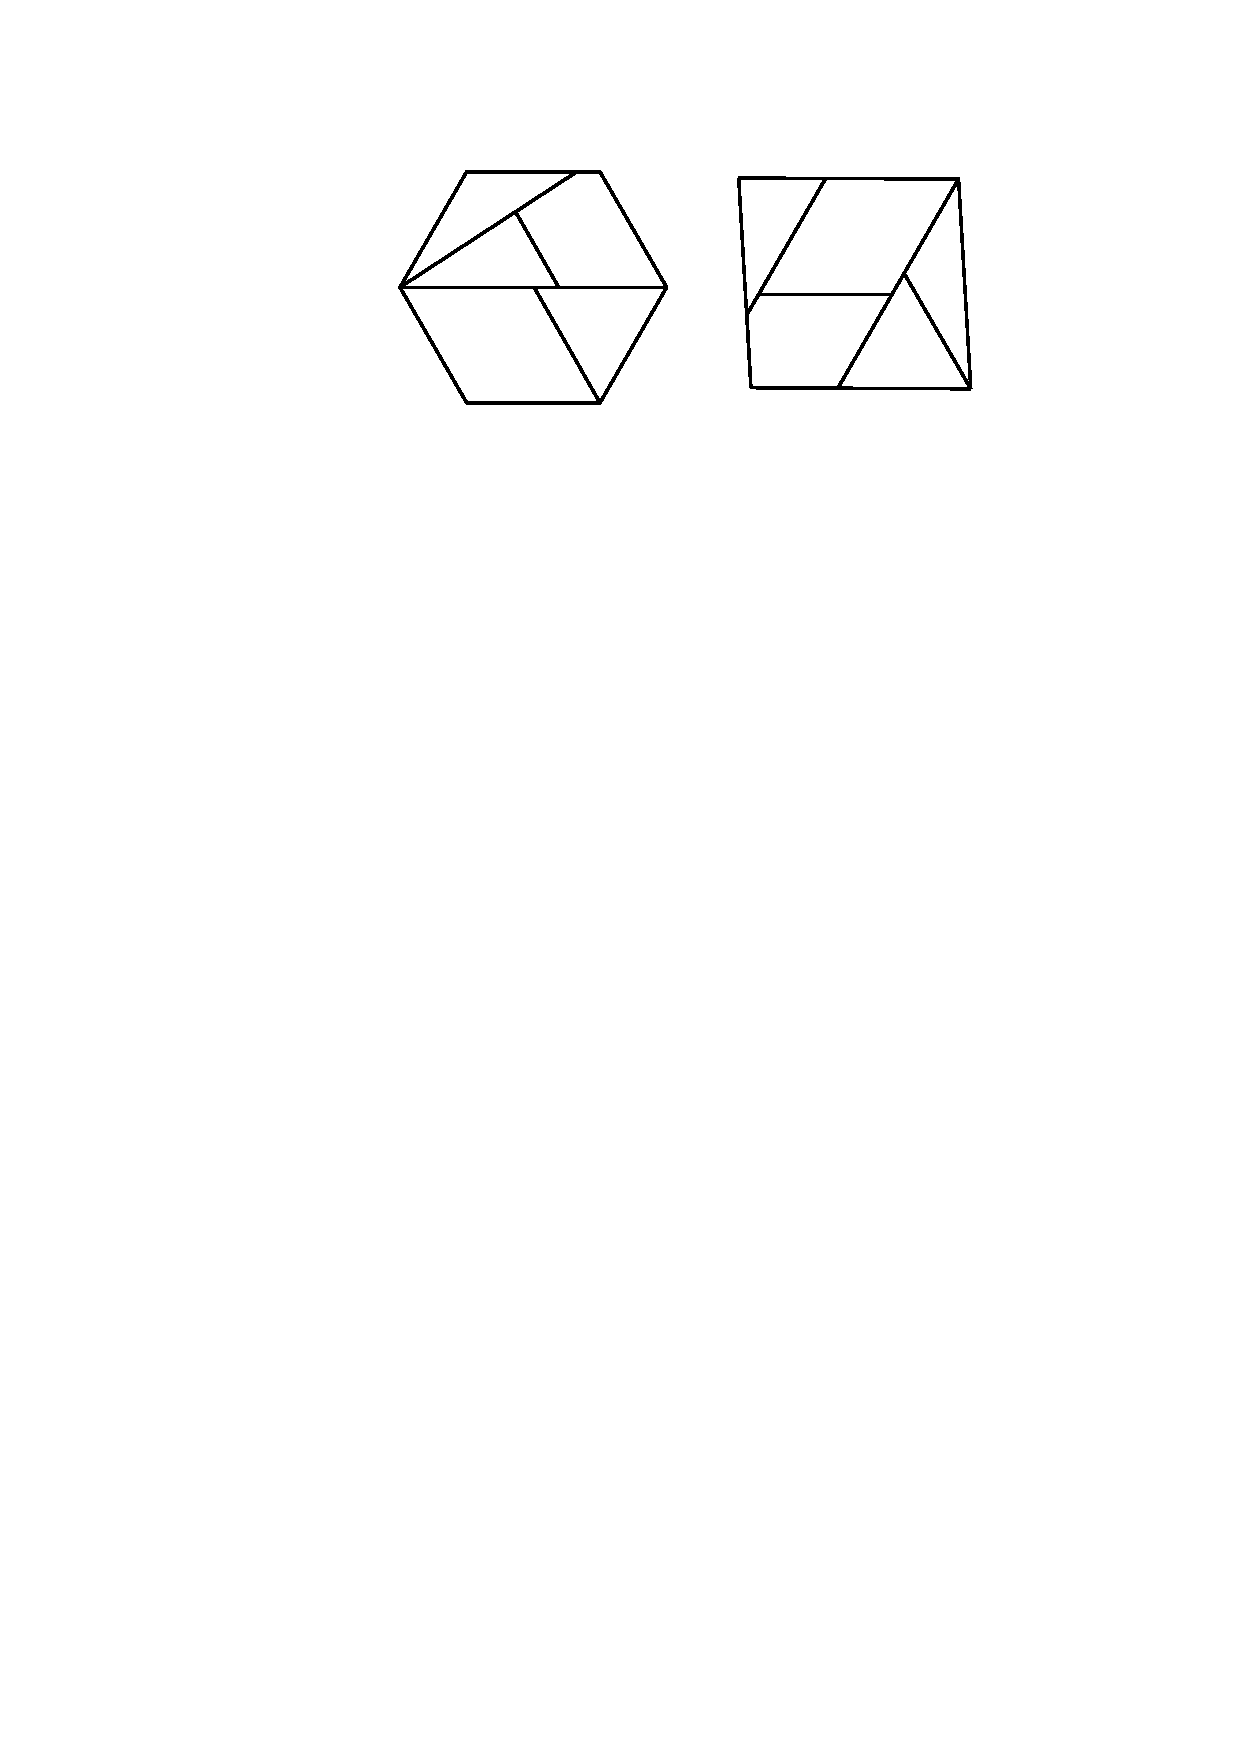
\includegraphics{graphics/GeometricDissectionBusschop.pdf}
\end{center}
\captionof{figure}{Two configurations of polygonal linkage where the polygons touch on boundary segments 
instead of hinges.  These two realizations of the polygonal linkage are invalid to our definitions. 
 }
\label{fig:polygonallinkage-4}
\end{minipage}

Figure \ref{fig:HingedHaberdasher}, shows the Haberdasher problem with hinges.  
This makes the Haberdasher problem as a type of polygonal linkage where the polygons are free to move about their hinge points and take the form of a triangle or square.  

\begin{minipage}{\linewidth}
\begin{center}
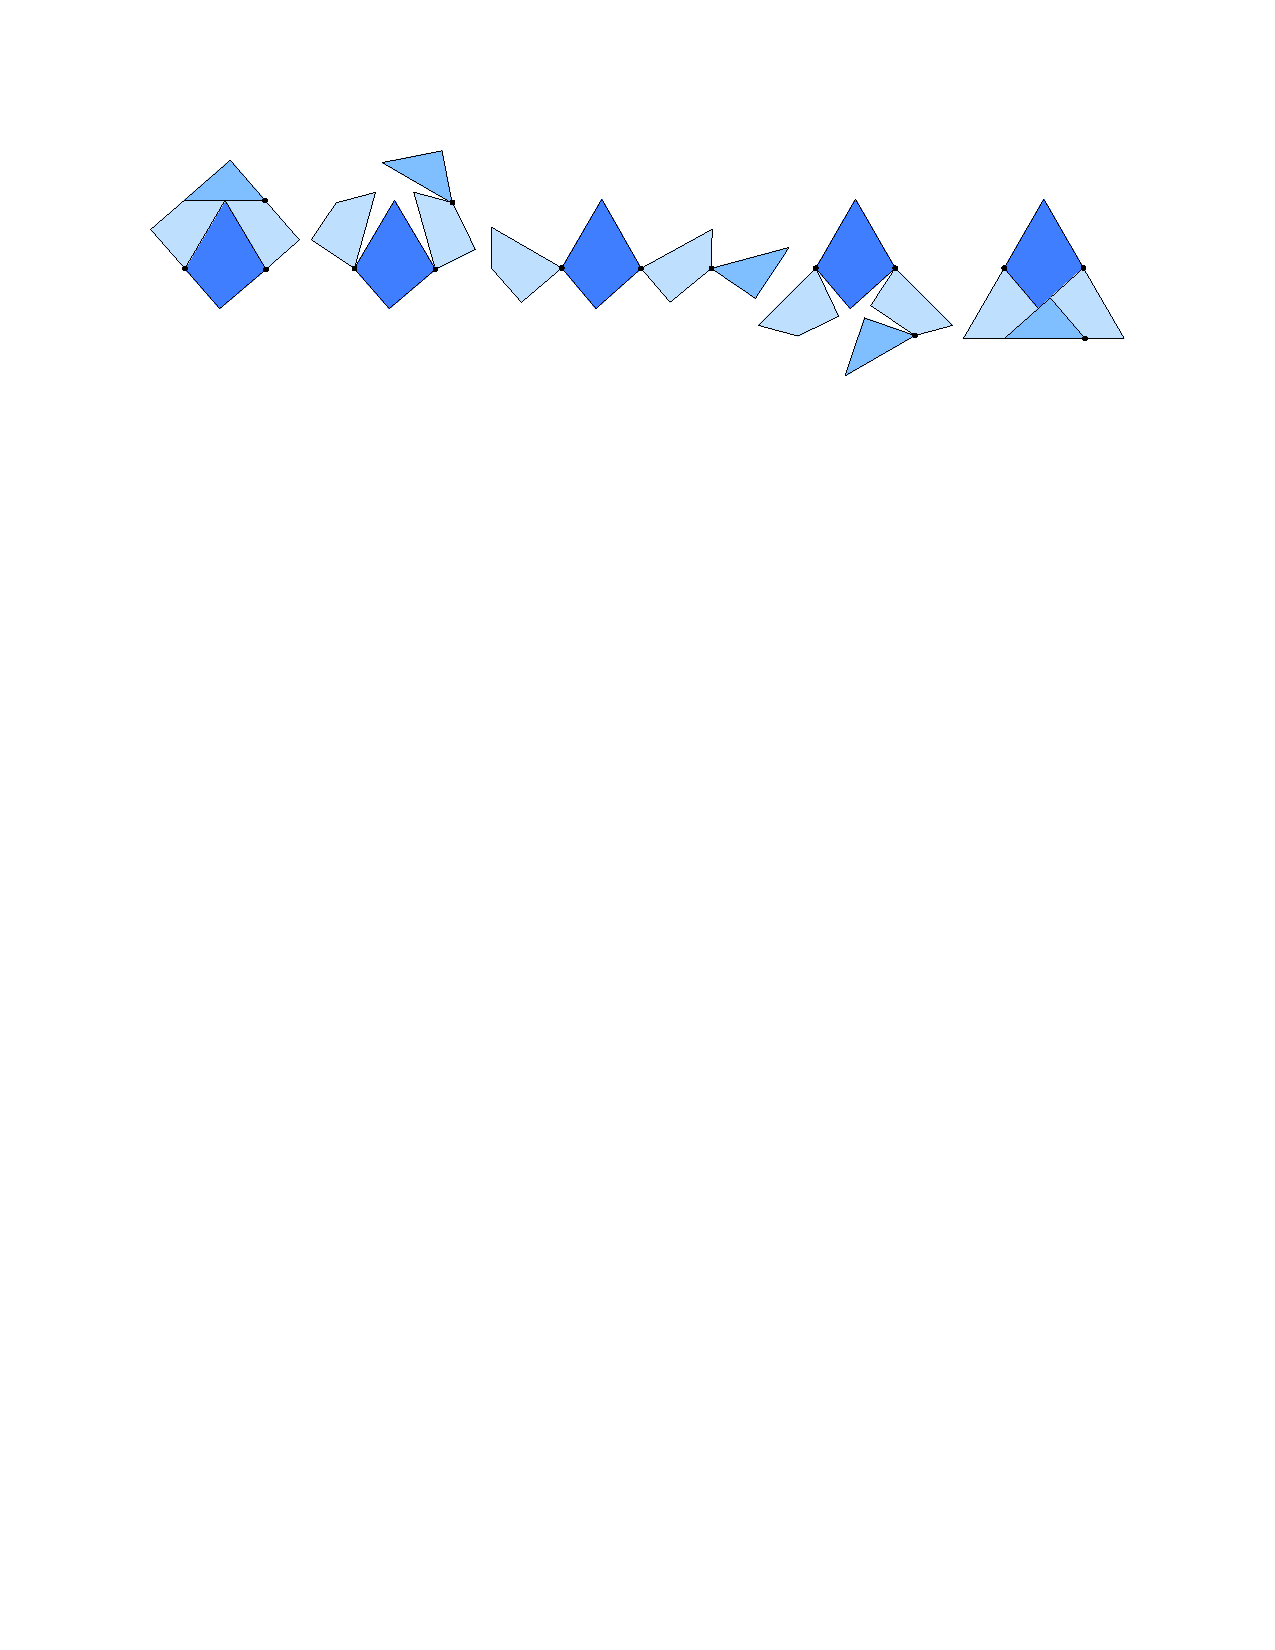
\includegraphics[width=\textwidth]{graphics/HingedHaberdasher.pdf}
\end{center}
\captionof{figure}{This shows the Haberdasher problem in the form of polygonal linkage \cite{abbott2012hinged}.  This is a classic example of two polygons of equal area that have a common hinged dissection.}
\label{fig:HingedHaberdasher}
\end{minipage}




% With three cuts, dissect an equilateral triangle into a square. The problem was first proposed by Dudeney in 1902, and subsequently discussed in Dudeney (1958), and Gardner (1961, p. 34), Stewart (1987, p. 169), and Wells (1991, pp. 61-62). The solution can be hinged so that the four pieces collapse into either the triangle or the square. Two of the hinges bisect sides of the triangle, while the third hinge and the corner of the large piece on the base cut the base in the approximate ratio 0.982:2:1.018.



% %%%%%%%%%%%%%%%%%%%%%%%%%%%%%%%%%%%%%%%%%%%%%%%%%%%%%%%%%%%%%%%%%%%%
% %%%%%%%%%%%%%%%%%%%%%%%%%%%%%%%%%%%%%%%%%%%%%%%%%%%%%%%%%%%%%%%%%%%%
% %%%%%%%%%%%%%%%%%%%%%%%%%%%%%%%%%%%%%%%%%%%%%%%%%%%%%%%%%%%%%%%%%%%%
% %%%%%%%%%%%%%%%%%%%%%%%%%%%%%%%%%%%%%%%%%%%%%%%%%%%%%%%%%%%%%%%%%%%%
% %%%%%%%%%%%%%%%%%%%%%%%%%%%%%%%%%%%%%%%%%%%%%%%%%%%%%%%%%%%%%%%%%%%%
% %%%%%%%%%%%%%%%%%%%%%%%%%%%%%%%%%%%%%%%%%%%%%%%%%%%%%%%%%%%%%%%%%%%%
% %%%%%%%%%%%%%%%%%%%%%%%%%%%%%%%%%%%%%%%%%%%%%%%%%%%%%%%%%%%%%%%%%%%%
% \begin{figure}[h]
% \begin{center}
% 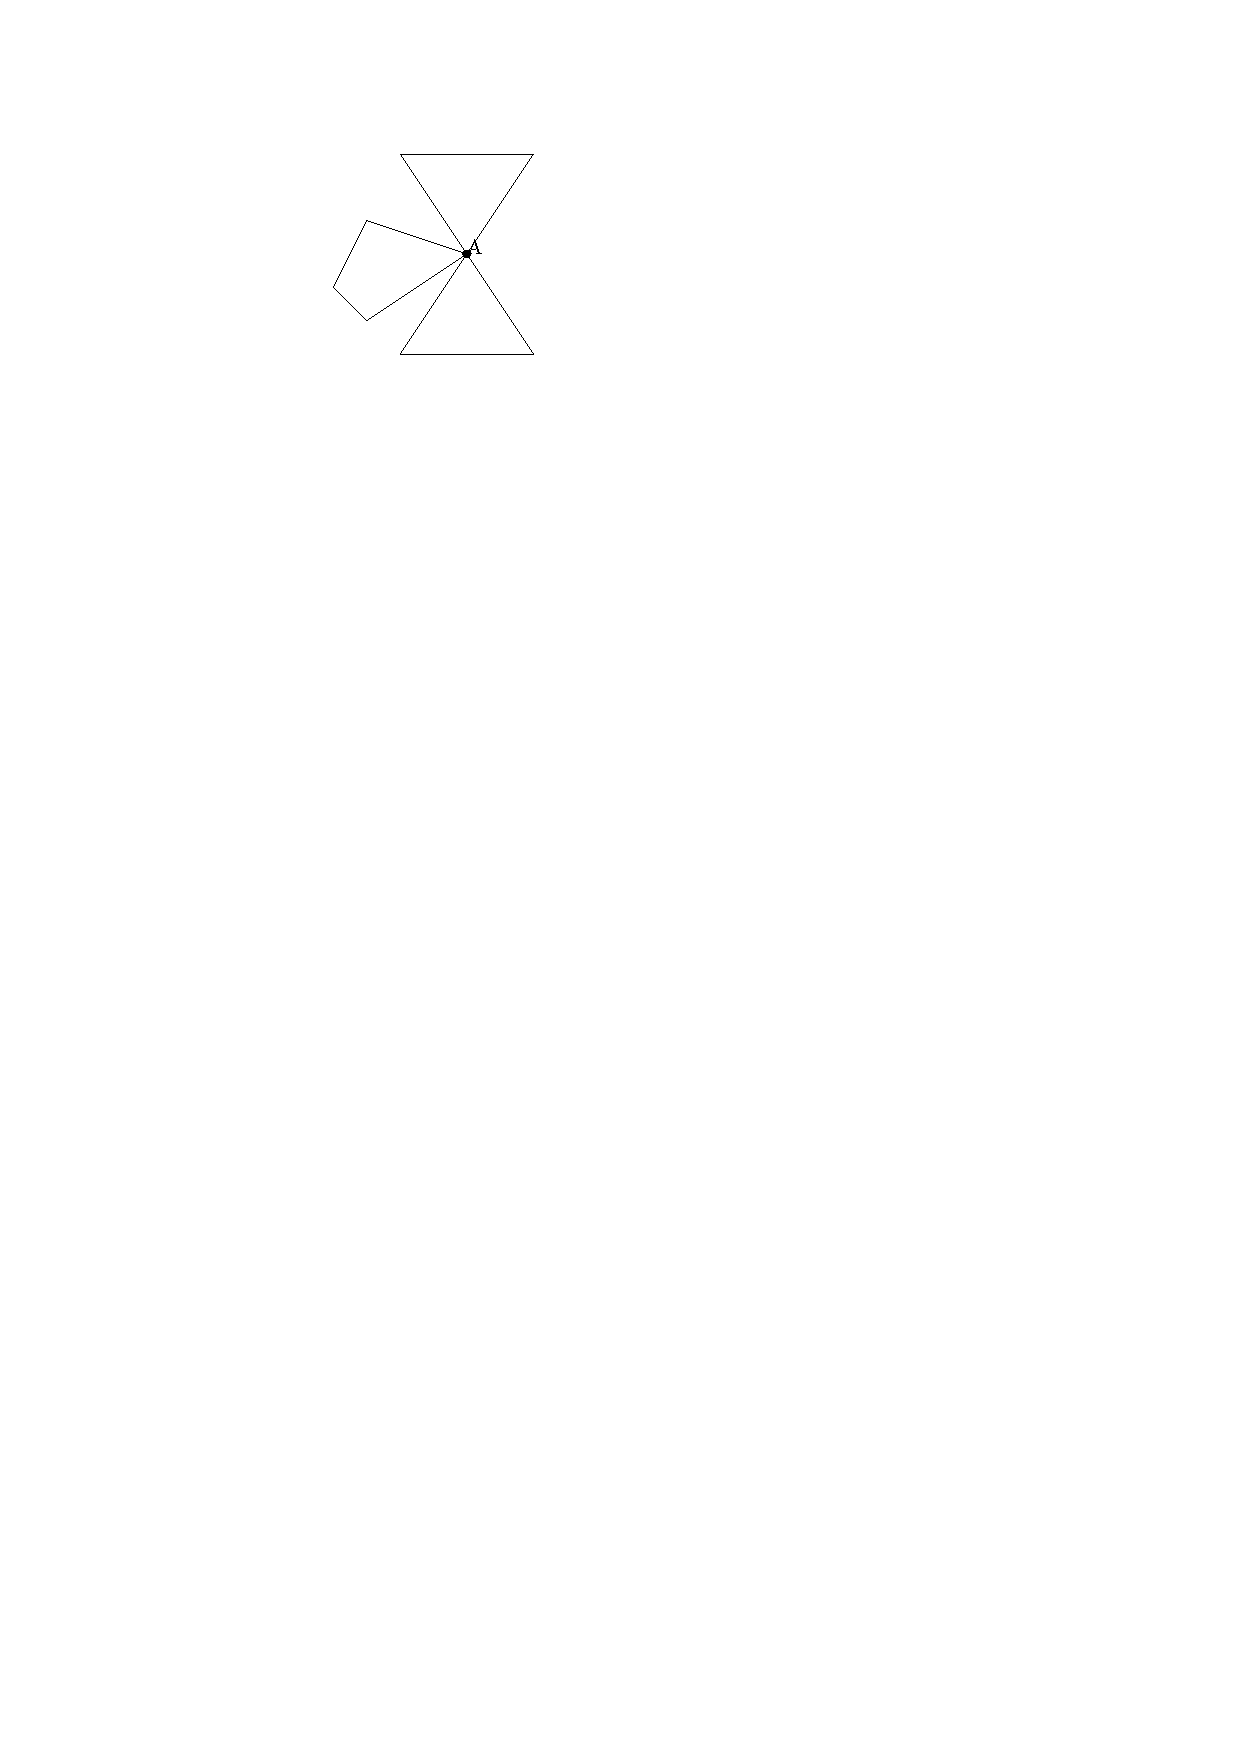
\includegraphics[scale=1]{graphics/hingeOnThreeDistinctPolygons.pdf}
% \end{center} 
% \caption{(a) A polygonal linkage with a non-convex polygon and two hinge points corresponding to 
% three polygons.  Note that hinge points correspond to two distinct polygons.(b) Illustrating that 
% two hinge points can correspond to the same boundary point of a polygon.}
% \label{fig:linkage-1}
% \end{figure}
% %describe how it is a generalization of Linkages.
% A generalization of linkages are polygonal linkages where the edges of given lengths are replaced 
% by rigid polygons.  Formally, a \textit{polygonal linkage} is an ordered pair $\left(\PP,\HH 
% \right)$ where $\PP$ is a finite set of polygons and $\HH$ is a finite set of hinges; a 
% \textit{hinge} $h\in \HH$ 
% corresponds to two points on the boundary of two distinct polygons in $\PP$.  A \emph{realization} 
% of a polygonal linkage is an interior-disjoint placement of 
% congruent copies of the polygons in $\PP$ such that the points corresponding to each hinge are 
% identified (Fig. \ref{fig:1}). 
% A \textbf{realization with orientation} uses only translated or rotated copies of the polygons in $\PP$ (no reflections) and for each hinge, the cyclic order of incident polygons is given. 
% The topology of a polygonal linkage can be represented by the \textbf{hinge graph}, a bipartite graph where the vertices correspond to polygons in $\PP$ and the hinges in $H$, and edges represent the polygon-hinge incidences.
% This definition of realization rules well known geometric 
% dissections (e.g. Fig. \ref{fig:polygonallinkage-4}).
% %this is where the geometric dissection figure belongs
% \begin{figure}[h]
% \begin{center}
% 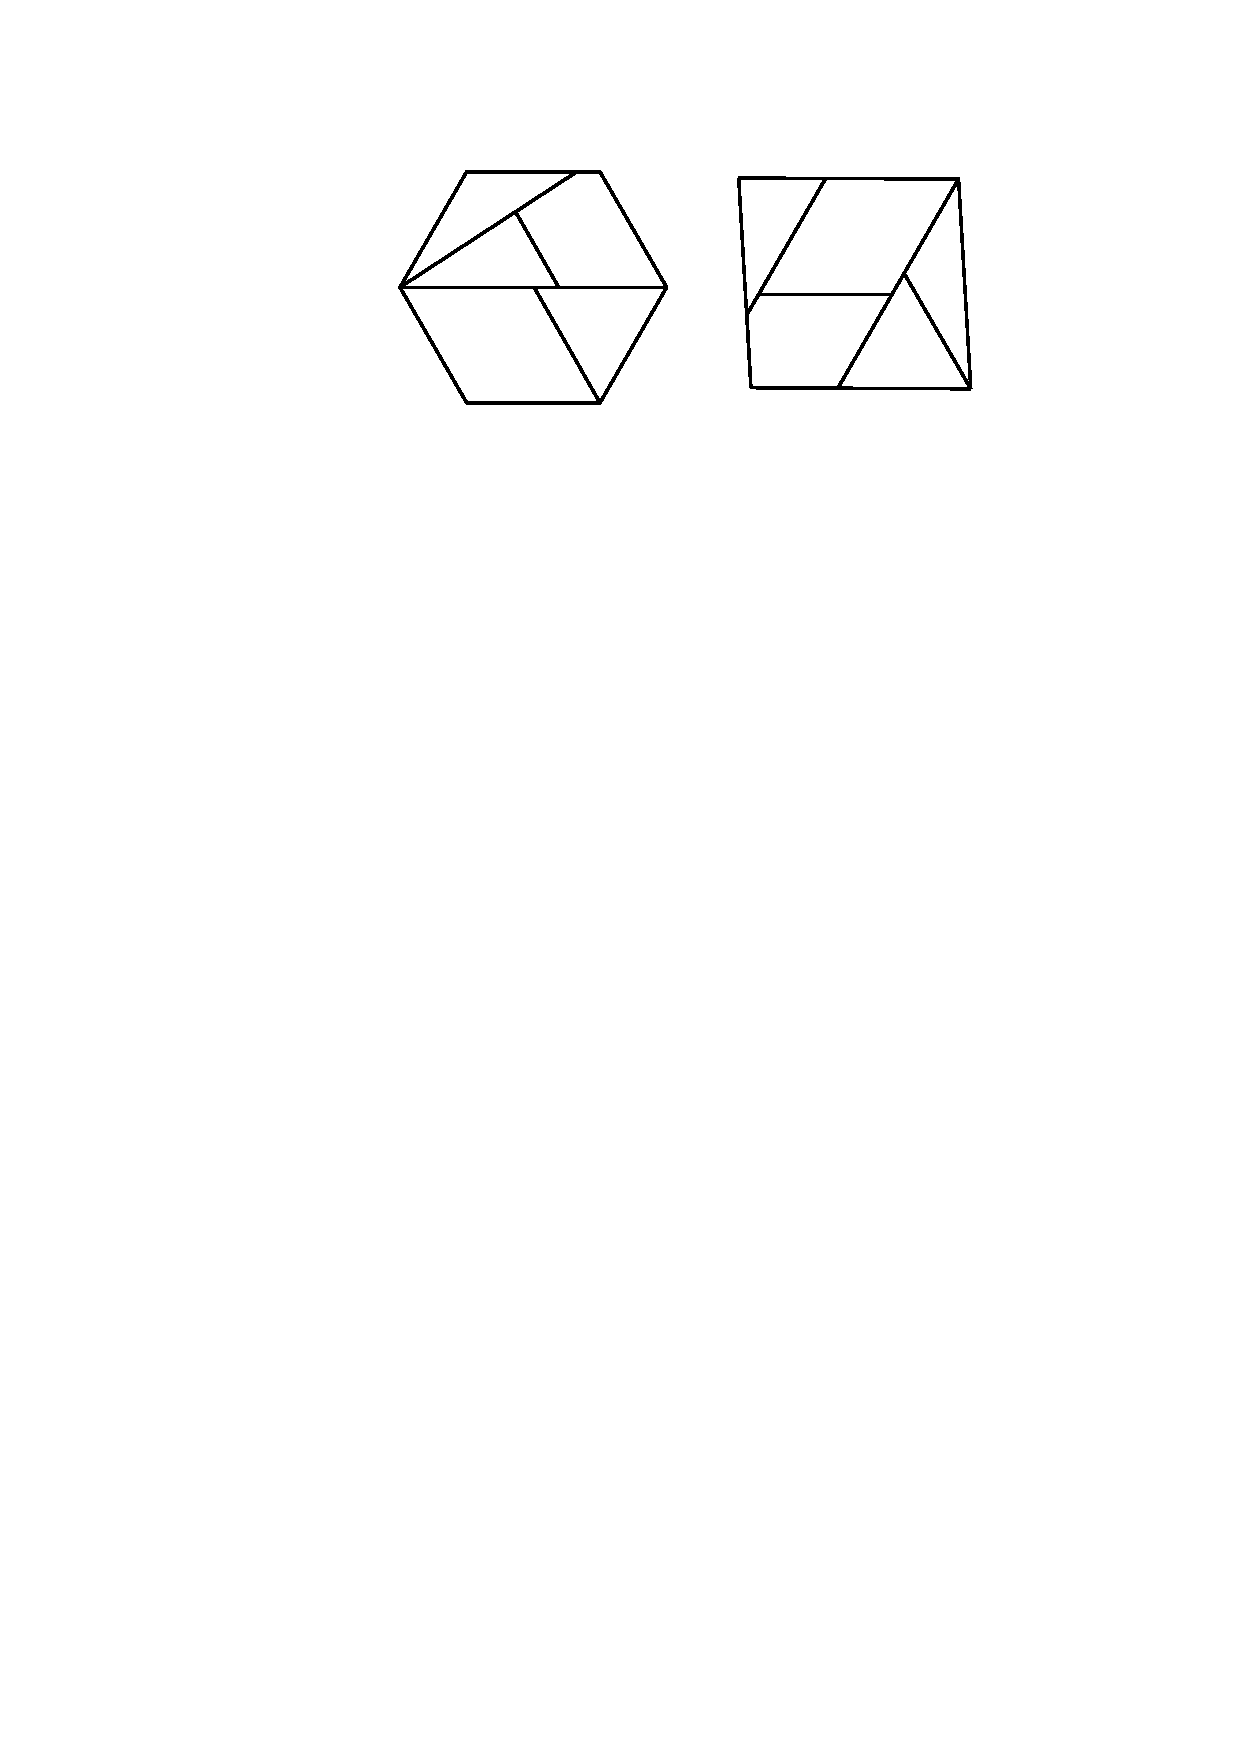
\includegraphics{graphics/GeometricDissectionBusschop.pdf}
% \end{center}
% \caption{Two configurations of polygonal linkage where the polygons touch on boundary segments 
% instead of hinges.  These two realizations of the polygonal linkage are invalid to our definitions. 
%  }
% \label{fig:polygonallinkage-4}
% \end{figure}

% \begin{figure}[h]
% \begin{center}
% 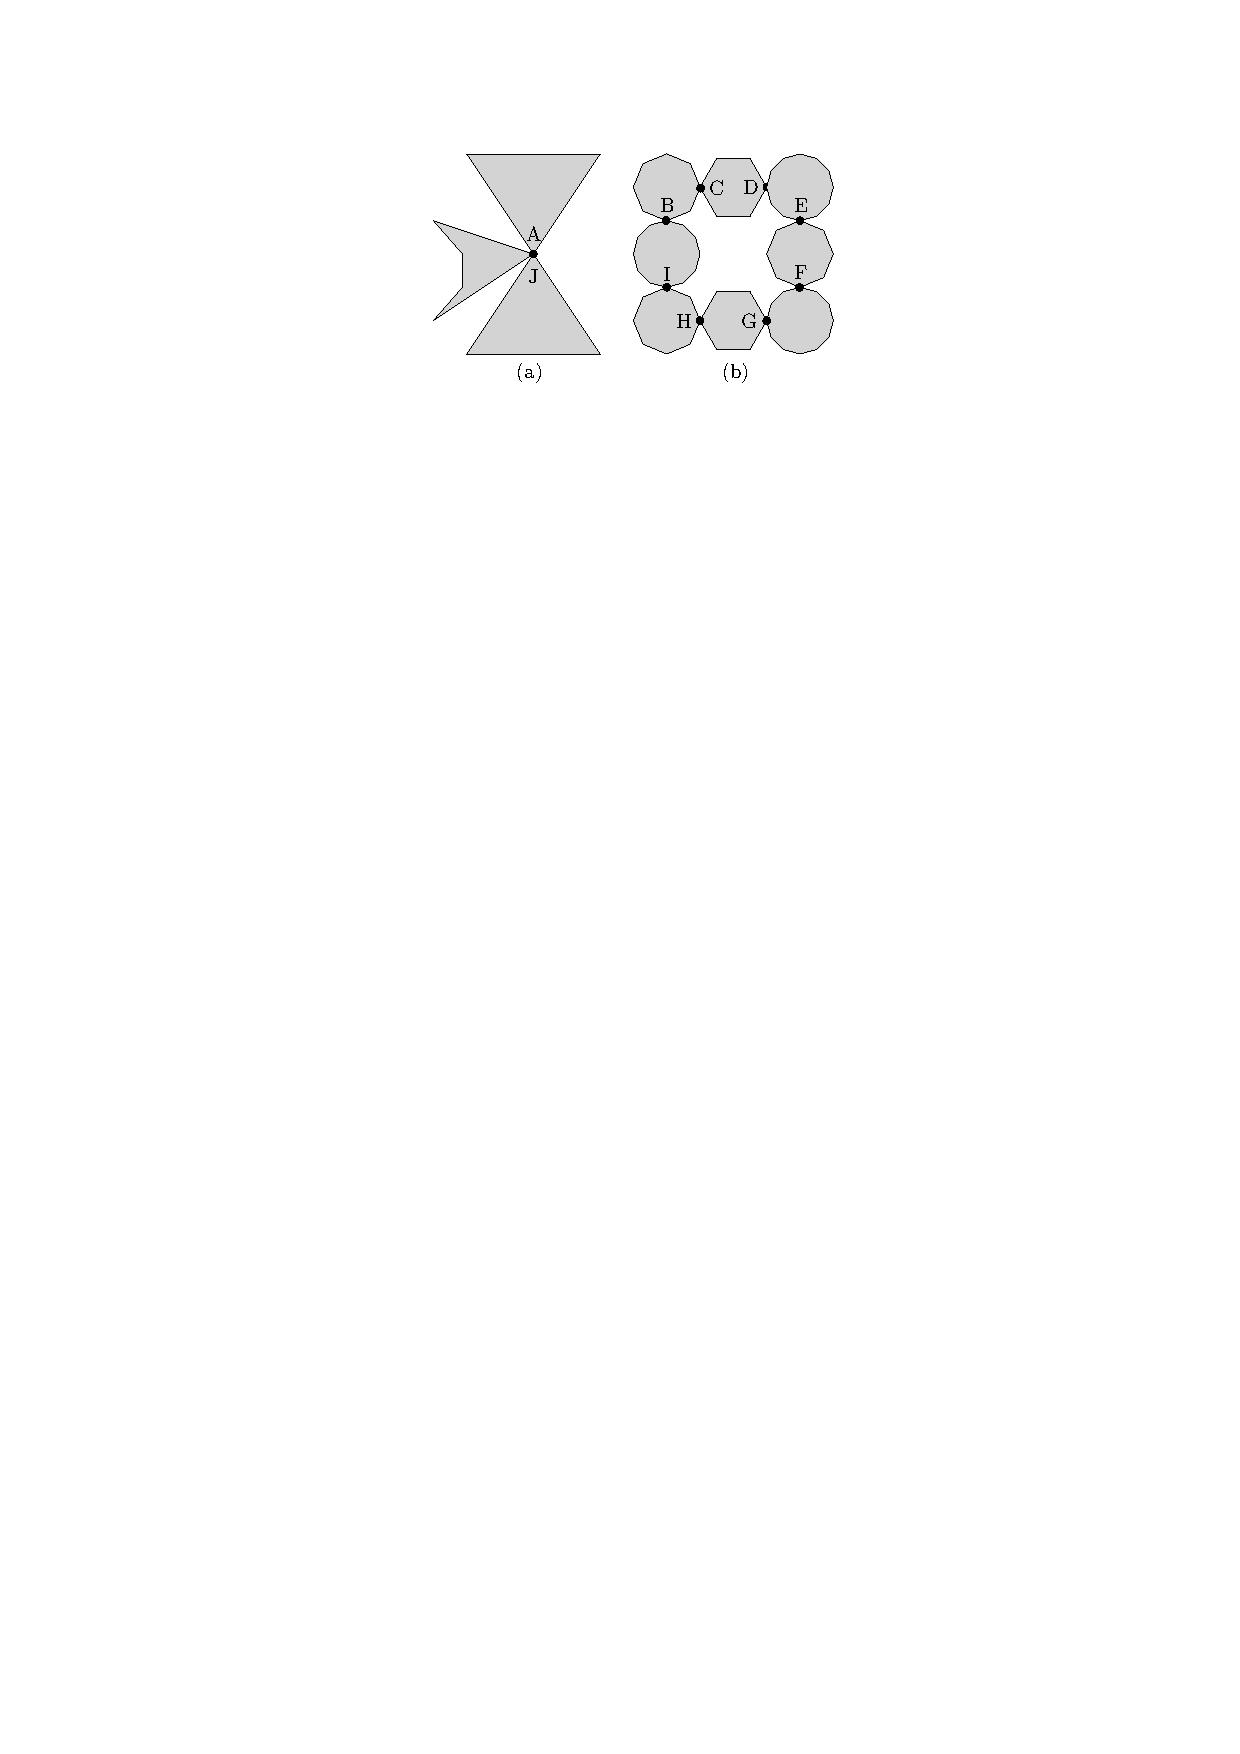
\includegraphics[scale=1]{graphics/linkageillustration.pdf}
% \end{center} 
% \caption{(a) A polygonal linkage with a non-convex polygon and a hinge point corresponding to three 
% polygons.  (b) A polygonal linkage with 8 regular polygons.}
% \label{fig:linkage-2}
% \end{figure}
% %%%%%%%%%%%%%%%%%%%%%%%%%%%%%%%%%%%%%%%%%%%%%%%%%%%%%%%%%%%%%%%%%%%%
% %%%%%%%%%%%%%%%%%%%%%%%%%%%%%%%%%%%%%%%%%%%%%%%%%%%%%%%%%%%%%%%%%%%%
% %%%%%%%%%%%%%%%%%%%%%%%%%%%%%%%%%%%%%%%%%%%%%%%%%%%%%%%%%%%%%%%%%%%%
% %%%%%%%%%%%%%%%%%%%%%%%%%%%%%%%%%%%%%%%%%%%%%%%%%%%%%%%%%%%%%%%%%%%%
% %%%%%%%%%%%%%%%%%%%%%%%%%%%%%%%%%%%%%%%%%%%%%%%%%%%%%%%%%%%%%%%%%%%%
% %%%%%%%%%%%%%%%%%%%%%%%%%%%%%%%%%%%%%%%%%%%%%%%%%%%%%%%%%%%%%%%%%%%%
% %%%%%%%%%%%%%%%%%%%%%%%%%%%%%%%%%%%%%%%%%%%%%%%%%%%%%%%%%%%%%%%%%%%%

% For the remainder of this thesis, we'll focus on the polygonal linkages with the following 
% restrictions:
% \begin{enumerate}
% \item Embedded polygons must be convex, i.e. for any two embedded points $u,v \in P'$, the set:
% $$\left\lbrace u  \cdot t + (1-t) \cdot v : t \in [0,1] \right\rbrace \in P'$$
%  \item  Polygons can only intersect at hinge points.  No two polygons can intersect at 
% their boundary or interior with the exception of possible a hinge point.  
% \end{enumerate}% 1.1.3. Disk graphs and problem definitions

% For the sake of simplicity, throughout this thesis we often refer to disks and their corre- sponding vertices synonymously. For example, we might simply say ’we create a disk D2 with radius r2 that touches disk D1’ instead of saying ’we create a vertex v2, a correspond- ing disk D2 with radius r2 and an edge between v2 and vertex v1 whose corresponding disk is D1’.
% Let G = (V, E) be a graph. We say that G has a realization as a disk intersection (touching) graph, if there exist a set of disks V and a bijection from V to V such that G = (G,V) is a disk intersection (touching) graph. In this case, we say G realizes G. Let Dv ∈ V be the disk of G corresponding to vertex v for any v ∈ V . A radius assignment for G is a function r : V → R+ that assigns a positive real number to each vertex of G. If the radius of disk Dv ∈ V is equal to r(v) for every v ∈ V , then G is said to respect r. A seed assignment for G is a function σ : V → R2 that assigns a point in the plane to each vertex ofG.Ifσ(v)∈Dv foreveryv∈V,thenGissaidtorespectσ.LetΓbeacombinatorial embedding for G. If G is a disk touching graph and if the cyclic order of disks touched by Dv corresponds to the cyclic order of edges incident to the vertex v for any v ∈ V , then G is said to respect Γ.
% We consider the following family of decision problems, in which the dots (...) are a place- holder for one, multiple or none of the enlisted variants.
% (Unit/ρ-bounded) Disk Intersection/Touching Graph Recognition (with ...): The problem instance is a graph G = (V, E) and the question is whether it is possible to realize G as a (unit/ρ-bounded) disk intersection/touching graph (which respects ...).
% • ... fixed Radii: ... a given radius assignment r for G.
% • ... fixed Embedding: ... a given combinatorial embedding Γ for G. • ... fixed Seeds: ... a given seed assignment σ for G.
% In particular, we consider the following problems:
% • Unit Disk Touching Graph Recognition (UDT)
% • Unit Disk Touching Graph Recognition with fixed Embedding (UDTE)
% • ρ-bounded Disk Touching Graph Recognition (ρ-BDT)
% • Disk Touching Graph Recognition with fixed Radii (DTR)
% • Disk Touching Graph Recognition with fixed Radii and Embedding (DTRE)
% • Disk Touching Graph Recognition with fixed Seeds (DTS)
% • Unit Disk Touching Graph Recognition with fixed Seeds (UDTS)
% • Unit Disk Touching Graph Recognition with fixed Seeds and Embedding (UDTSE)
% 1.2. Related work
% As mentioned in the beginning of this chapter, Koebe’s Theorem [Koe36] implies that the Disk Touching Graph Recognition problem can be solved in linear time. On the other hand, Hlinˇeny ́ and Kratochv ́ıl showed that the Disk Intersection Graph Recognition problem is NP-hard [HK01].
% A result by Breu and Kirkpatrick states that the Unit Disk Intersection/Touching Graph Recognition problems are NP-hard [BK98], implying that the Disk Intersection/Touching Graph Recognition with fixed Radii problems are also N P -hard. There exists some heuris- tics for generating disk touching graphs with fixed radii [Dor96, Ino11] for the application of cartogram generation.
% 6
% Breu and Kirkpatrick generalized their results by showing that the ρ-bounded Disk Inter- section/Touching Graph Recognition problems are NP-hard for any fixed ρ ≥ 1 [BK96]. Alam et al. [AEG+14] argue that for any tree, for any cactus (which is a connected graph in which each edge is contained in at most one cycle), for any k-outerplanar graph with bounded maximum degree and k ∈ O(log n) and for any planar graph with bounded tree- depth there exists a realizing ρ-bounded disk touching graph where ρ is a polynomial in the number of vertices.
% Atienza et al. show that the Disk Touching Graph Recognition with fixed Seeds problem is NP-hard [AdCC+12].








\section{Disk Arrangements\label{sec:disk}}
%Circle packing theorem: For every connected simple planar graph G there is a circle packing in the plane whose intersection graph is (isomorphic to) G.
% A disk D is a region in the plane bounded by a circle. A disk can be uniquely described by its bounding circle’s radius r ∈ R+ and center c ∈ R2. A disk is called closed if it contains the points of its bounding circle and open otherwise. A disk intersection graph G = (G, V) consists of a graph G = (V,E), a set of closed disks V and a bijection from the set of vertices V to V such that two vertices of V are adjacent in G if and only if their corresponding disks in V intersect. A disk touching graph G = (G, V) is a disk intersection graph such that the interiors of the disks in V are pairwise disjoint. The centers of the disks in V together with straight-line segments that connect the centers of all pairs of touching disks induce a planar drawing of G. In a unit disk intersection (touching) graph all disks share one uniform radius. In a ρ-bounded disk intersection (touching) graph the radius of all disks is taken from the interval [1, ρ] for a value ρ ≥ 1. Note, that a 1-bounded disk intersection (touching) graph is a unit disk intersection (touching) graph.

 A \textit{disk arrangement} is a set of interior disjoint disks, $D$.  
 If for any pair of disks in $D$ intersect at a boundary point, they are said to be in contact (kissing).

\begin{minipage}{\linewidth}
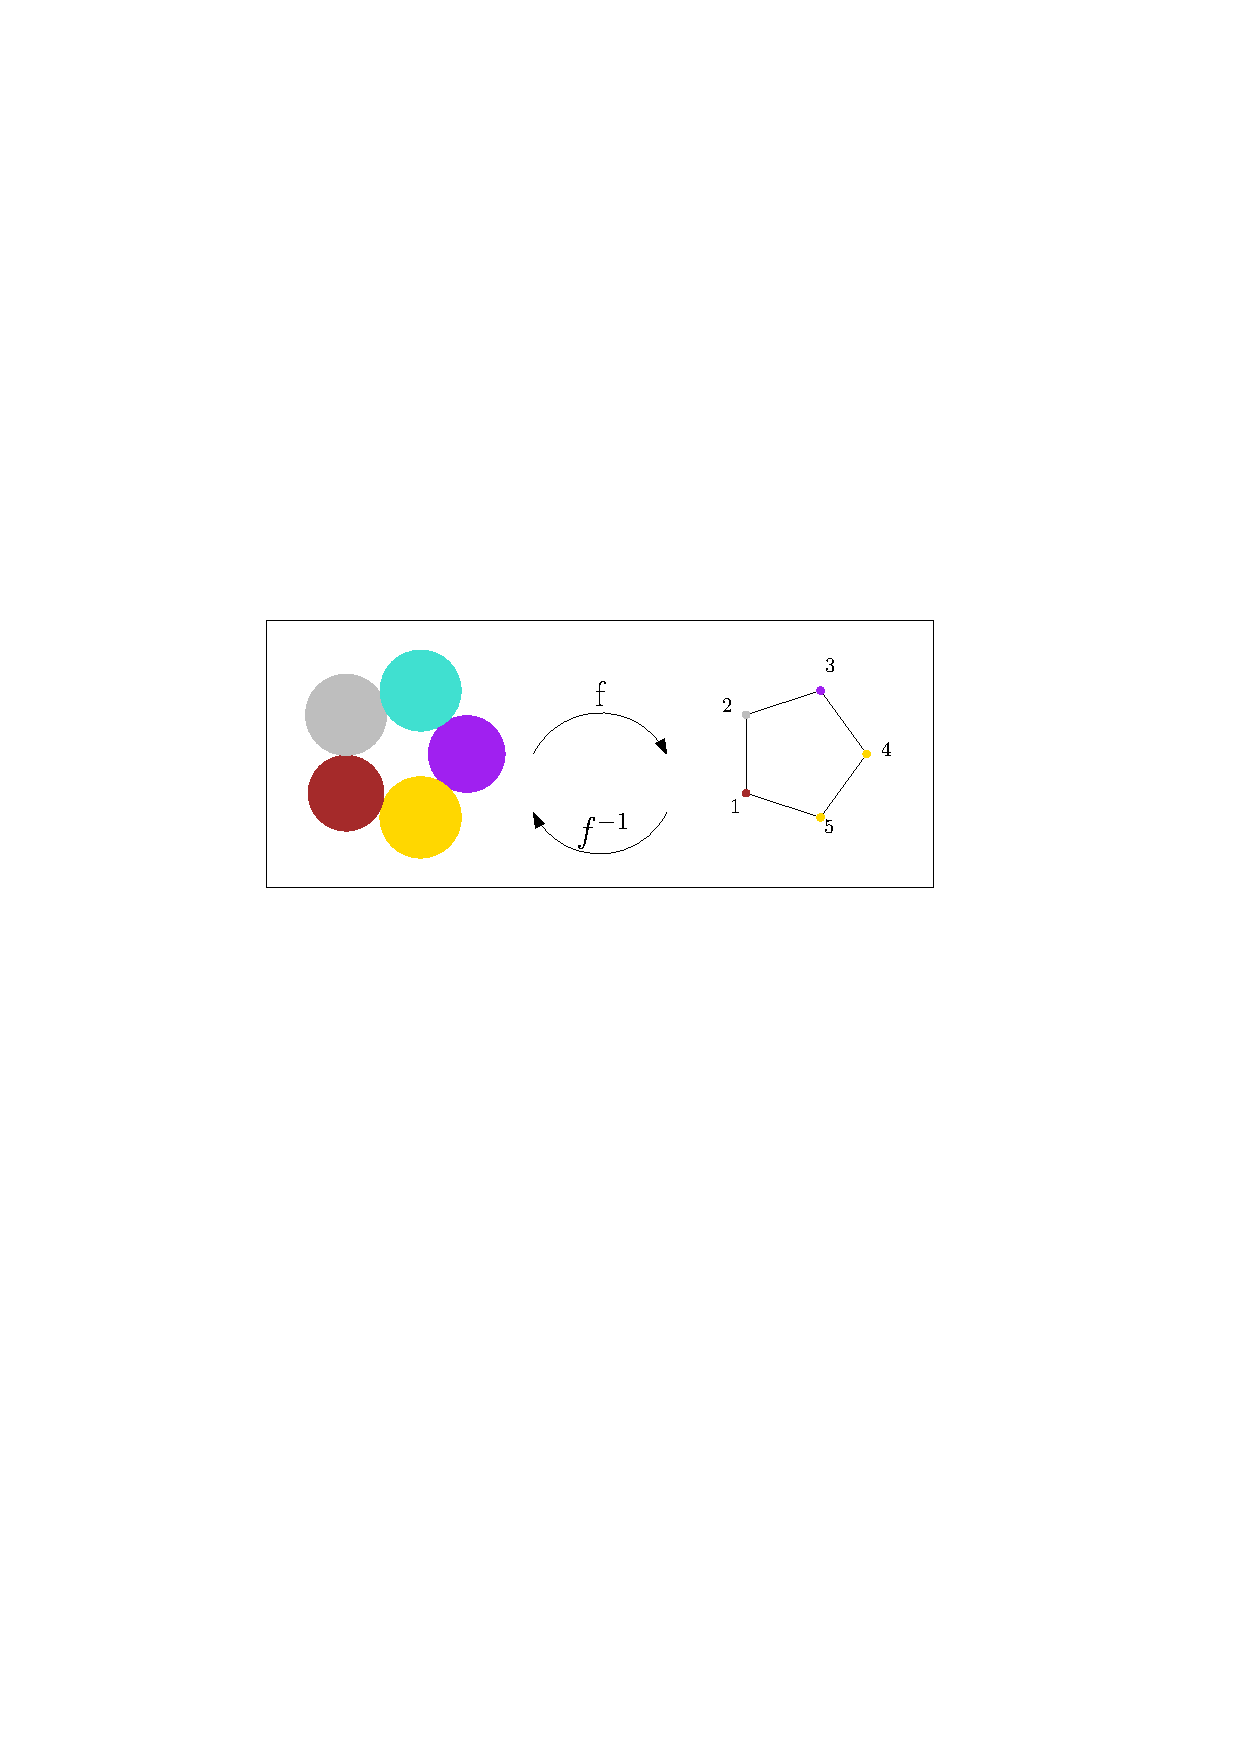
\includegraphics[scale=1]{graphics/diskPackingTheoremExample.pdf}
\captionof{figure}{This example represents a disk arrangement and its contact graph.}
\label{fig:DiskArrangement-1}
\end{minipage}

A \textit{contact graph} $G=(V,E)$ corresponding to a given disk arrangement where there is a bijection $b_V: V \mapsto D$ and a bijection that maps an edge $e_{i,j} \in E$ to an interior disjoint pair of disks $d_i$, $d_j \in D$ (see Figure \ref{fig:DiskArrangement-1}).
Given a disk arrangement, the contact graph can be thought of as a linkage because the distance between two kissing disk equal the sum of radii.  
However if the two disks don't kiss, the distance between their centers is strictly greater than the sum of their radii.
Given a disk arrangement, the contact graph can be thought of as a linkage because the distance between two kissing disk equal the sum of radii.  
However if the two disks don't kiss, the distance between their centers is strictly greater than the sum of their radii.

Koebe's theorem states that for every planar graph $G$, there exists a planar disk arrangement whose contact graph is $G$ \cite{koebe1936kontaktprobleme}.
This motivates the question of whether a planar graph $G$ is a contact graph of a disk arrangement with given radii.
The radii can be given by a weight function.
Let $\omega: V \mapsto \bbR^+$ be the \textit{weight function}.  
$\omega$ assigns a weight to each vertex in $V$.  
Let $\Pi:V \mapsto \bbr^2$ be that planar mapping of vertices.
%$D$ \textit{respects radii assignments} if for every $v \in V$ such that $b_V(v) = D_v$, $\omega(v)$ is the radius of $D_v$.    
%$D$ \textit{respects center assignments} if for every $v \in V$, $\Pi(v)$ is the center of $D_v$.  
%Note that if $\omega$ respects radii assignments, then it can be equivelently said that the linkage $(G,\ell)$ with length assignment $\ell$ also respects radii assignments.  
%In this thesis, unless otherwise stated we assume that the contact graph associates to an $\omega$ and $\Pi$ mapping that respect radii and center assignments.
%we may also interchange contact graph with linkage.



% For the sake of simplicity, throughout this thesis we often refer to disks and their corre- sponding vertices synonymously. For example, we might simply say ’we create a disk D2 with radius r2 that touches disk D1’ instead of saying ’we create a vertex v2, a correspond- ing disk D2 with radius r2 and an edge between v2 and vertex v1 whose corresponding disk is D1’.
% Let G = (V, E) be a graph. We say that G has a realization as a disk intersection (touching) graph, if there exist a set of disks V and a bijection from V to V such that G = (G,V) is a disk intersection (touching) graph. In this case, we say G realizes G. Let Dv ∈ V be the disk of G corresponding to vertex v for any v ∈ V . A radius assignment for G is a function r : V → R+ that assigns a positive real number to each vertex of G. If the radius of disk Dv ∈ V is equal to r(v) for every v ∈ V , then G is said to respect r. A seed assignment for G is a function σ : V → R2 that assigns a point in the plane to each vertex ofG.Ifσ(v)∈Dv foreveryv∈V,thenGissaidtorespectσ.LetΓbeacombinatorial embedding for G. If G is a disk touching graph and if the cyclic order of disks touched by Dv corresponds to the cyclic order of edges incident to the vertex v for any v ∈ V , then G is said to respect Γ.
% %By Koebe's Theorem, every disk arrangement embedded in the plane has a contact graph.
% A \textit{contact graph} represents vertices as interior disjoint disks and by representing edges as as points of intersections (contact), \textit{kissing points} between two disks.  
% The graph corresponding to a given disk arrangement, $\DD$, is said to be the \textit{contact graph}. 
% An ordered disk arrangement preseves the  cyclic order of neighborings disks. 
% %A \it{disk arrangement} is a set, $\DD$, of pairwise interior-disjoint disks in the plane, 
% %$\DD=\left\lbrace C_i \right\rbrace_{i = 1}^n $.


%What is not obvious is when given a graph with positive weights, does there exist a planar drawing?
%Some variants of these problems were known to be NP-Hard.
For planar graphs with positive weighted vertices, we pose two realizability problems:
\begin{prob}[Unordered Realizibility Problem for a Contact Graph]\label{problem:UnorderedContactGraph}
Given a planar graph with positive weighted vertices, is it a contact graph of some disk arrangement where the radii equal the vertex weights?
\end{prob}
\begin{prob}[Ordered Realizibility Problem for a Contact Graph]\label{problem:OrderedContactGraph}
Given a planar graph with positive weighted vertices and a combinatorial embedding, is it a contact graph of some disk arrangement where the radii equal the vertex weights and the counter-clockwise order of neighbors of each disk is specified by the combinatorial embedding?
\end{prob}

An instance of Problem \ref{problem:UnorderedContactGraph} is shown in Figure \ref{fig:DiskArrangement-1} where the cycle graph $C_5$ is the contact graph of unit disks.
It is not difficult to see that there exists a planar graph with positive weights with no realizable disk arrangement.
Consider the a star graph with 6 leafs, each vertex with unit weight.
In any realization, the angle between two consecutive edges must be greater than $\frac{\pi}{3}$. 
The sum of 6 angles is $2 \pi$ however, the sum of 6 consecutive angles is greater than $2\pi$.
The contradiction shows that no realization is possible (refer to Figure \ref{figure:starweel}).
Note that with the wheel graph $W_7$ is realizable as a contact graph of unit disks.

Every path with arbitrary positive radii is realizable as a contact graph, place the vertices on a line.
We show that not all binary trees are realizable, even with unit disks.% of unit radii.
Consider the balanced binary trees of depth $i$ $\left\lbrace T_i \right\rbrace_{i=1}^\infty$ with unit weights on the vertices (see Figure \ref{fig:circlePacking-1}).
These trees are not realizable for sufficiently large $i$.
\begin{figure}[!htbp]\label{fig:circlePacking-1}
\begin{center}
    %add desired spacing between images, e. g. ~, \quad, \qquad etc.
    %(or a blank line to force the subfigure onto a new line)
  \begin{subfigure}[b]{0.21\textwidth}
	  \includegraphics[width=\textwidth]{graphics/BinaryTree1.pdf}
	  \caption{Binary tree $T_2$.}
	  \label{fig:circlePacking1-1}
  \end{subfigure}
  \begin{subfigure}[b]{0.21\textwidth}
	  \includegraphics[width=\textwidth]{graphics/BinaryTree2.pdf}
	  \caption{Binary tree $T_3$.}
	  \label{fig:circlePacking1-2}
  \end{subfigure}
  \begin{subfigure}[b]{0.21\textwidth}
	  \includegraphics[width=\textwidth]{graphics/BinaryTree3.pdf}
	  \caption{Binary tree $T_4$.}
	  \label{fig:circlePacking1-3}
  \end{subfigure}
  \begin{subfigure}[b]{0.21\textwidth}
	  \includegraphics[width=\textwidth]{graphics/BinaryTree4.pdf}
	  \caption{Binary tree $T_5$.}
	  \label{fig:circlePacking1-4}
  \end{subfigure}
  \caption{ We show the linkages $T_2$ through $T_5$ with distance 2 between adjacent vertices.  }
\end{center} 
\end{figure}
%To show that as $i \rightarrow \infty$, the corresponding disk arrangement will not have a drawing.  
%We construct the disk arrangement as follows: (1) place a disk of unit radius centered at origin; (2) for each disk continue to add two non-intersecting kissing disks of unit radius to it.  
%To illustrate, see Figure \ref{fig:circlePacking-1}:
Let $i$ be a positive integer and suppose that $T_i$ is a contact graph of unit disks.
The balanced binary tree $T_i$ has $2^i -1$ vertices.
The total area of the disks is $\left( 2^i -1 \right)^2 \cdot \pi$.
We now derive an upper bound for this area.
%Suppose the root of the disk arrangement is centered at origin.
Suppose the disk corresponding to the root of the tree is centered at the origin.
The centers of the disks at level $j$ are at a distance at most $2\cdot (j-1)$ away from the origin.
The centers of all disks are at distance at most $2 \cdot (i -1)$ away from the origin.
All unit disks are contained in a disk of radius $2i-1$ centered at the origin.
The total area of the disks is at most $(2i-1)^2$.
%Let the total area of the disks arrangement be the sum of the areas of the disks. 
A upper bound of the total area of the disk arrangement is the area of the bounding box of the disks.

\begin{figure}[!htpb]\label{fig:circlePacking-2}
\begin{center}
    %add desired spacing between images, e. g. ~, \quad, \qquad etc.
    %(or a blank line to force the subfigure onto a new line)
  \begin{subfigure}[b]{0.24\textwidth}
	  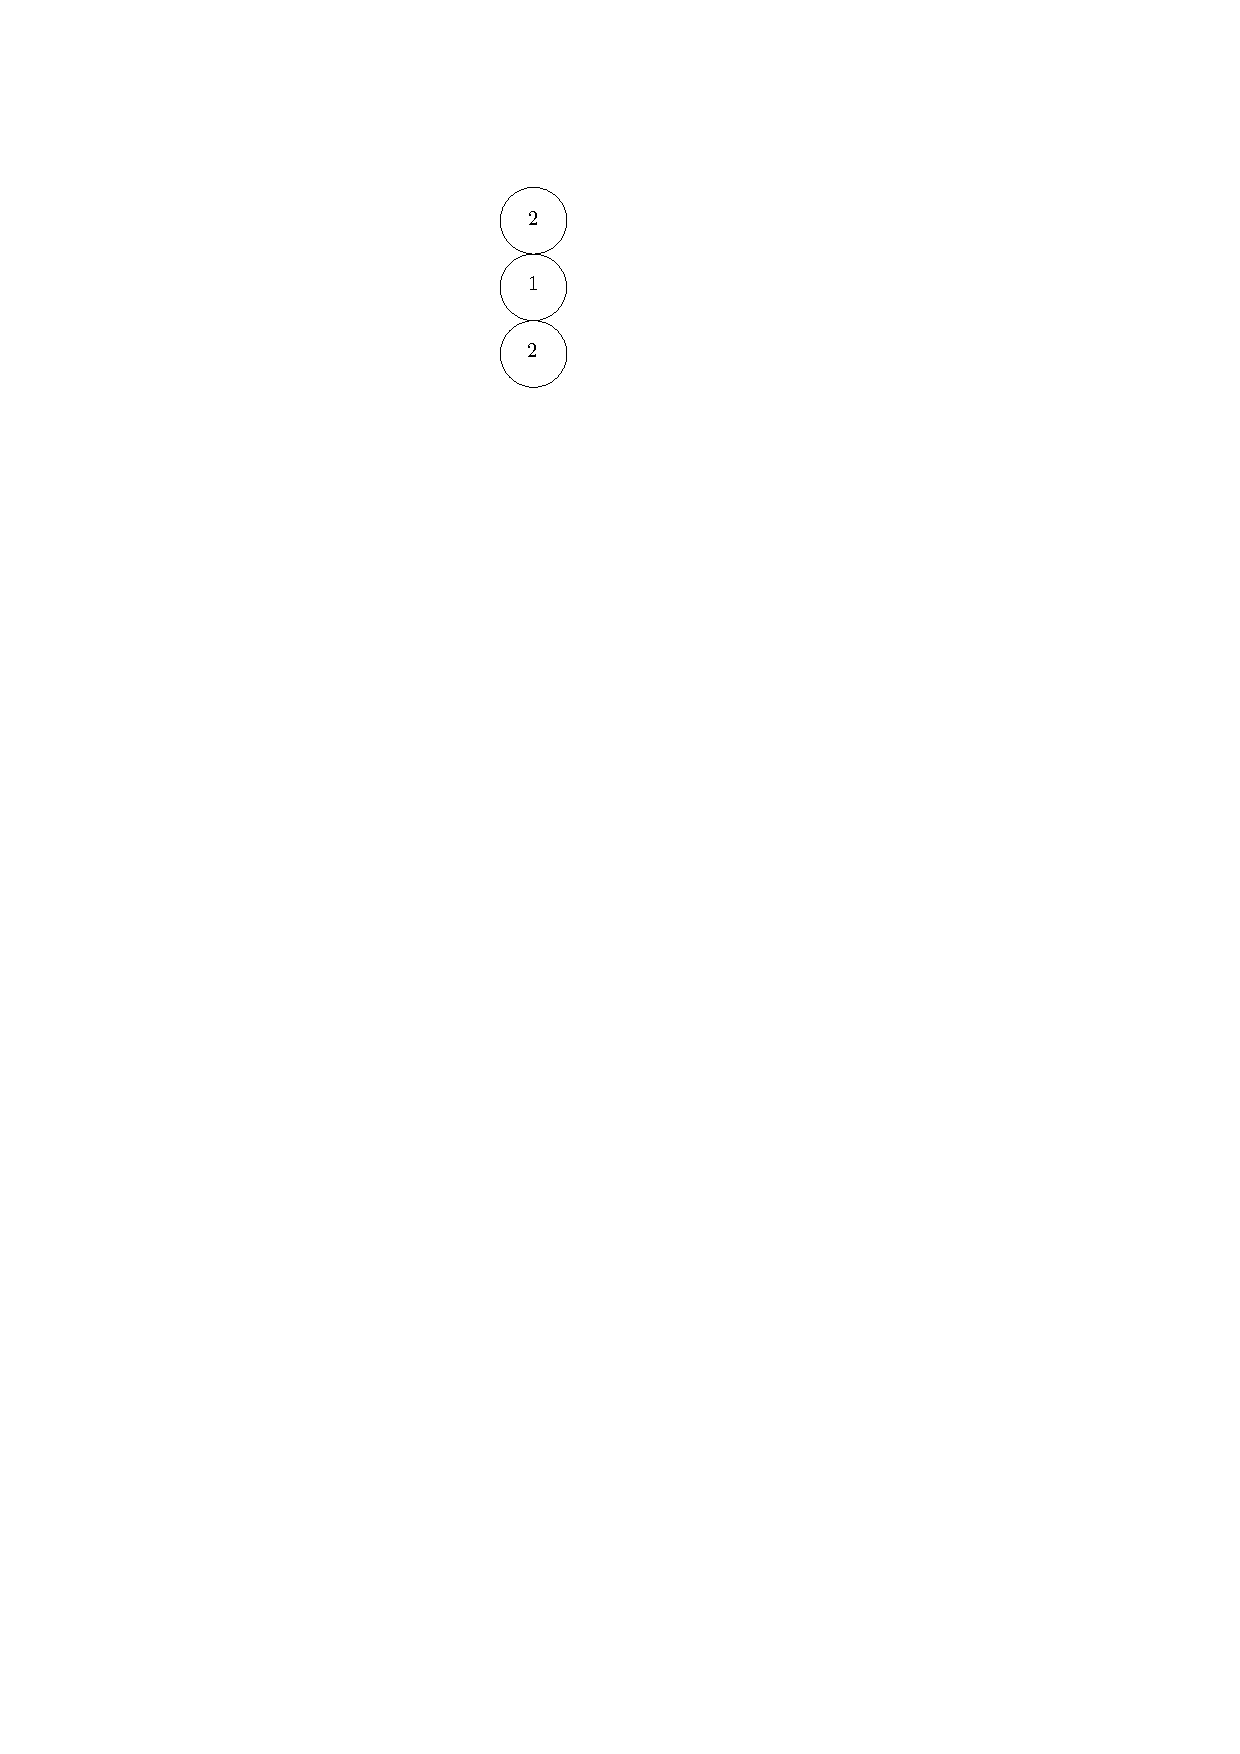
\includegraphics[width=\textwidth]{graphics/degree2arrangement.pdf}
	  \caption{A disk arrangement with two layers of disks}
	  \label{fig:circlePacking2-1}
  \end{subfigure}
  \begin{subfigure}[b]{0.24\textwidth}
	  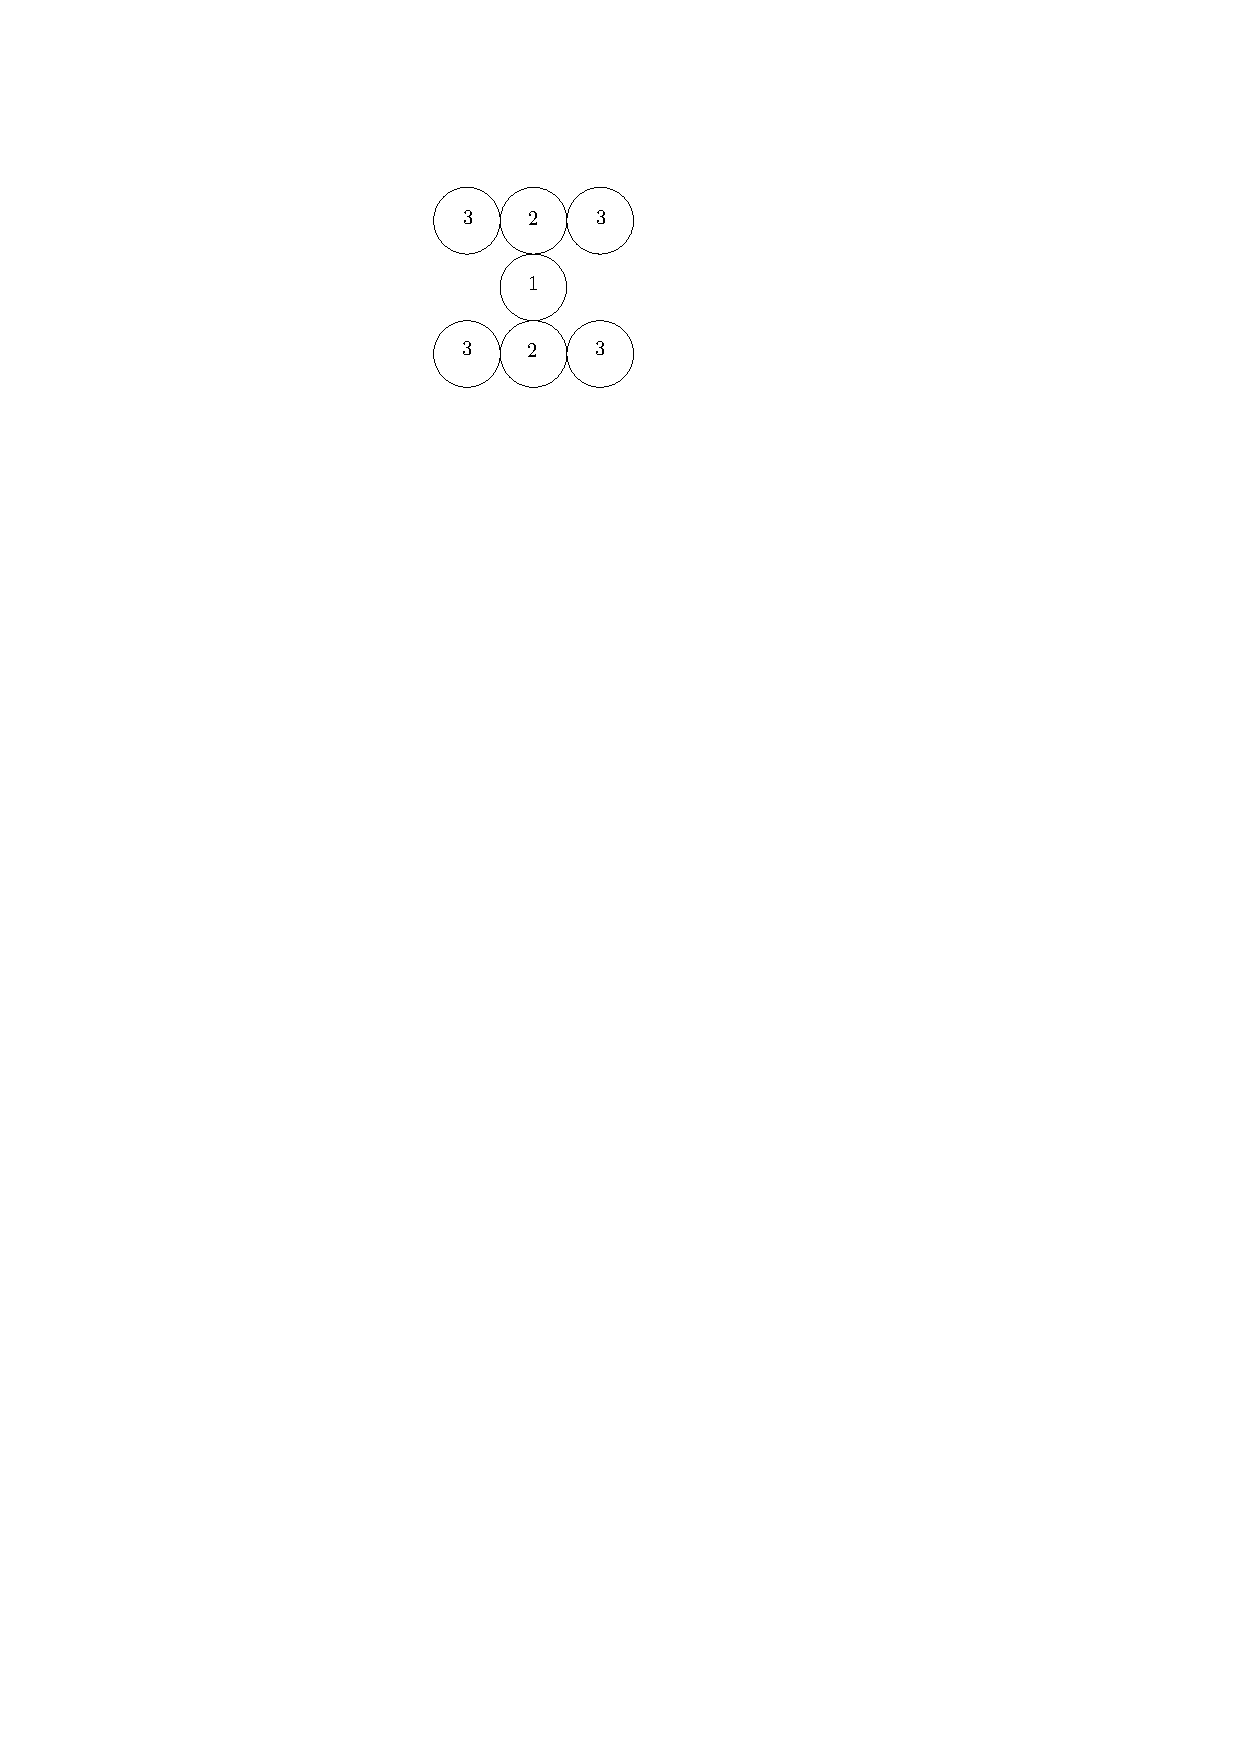
\includegraphics[width=\textwidth]{graphics/degree3arrangement.pdf}
	  \caption{A disk arrangement with three layers of disks}
	  \label{fig:circlePacking2-2}
  \end{subfigure}
  \begin{subfigure}[b]{0.24\textwidth}
	  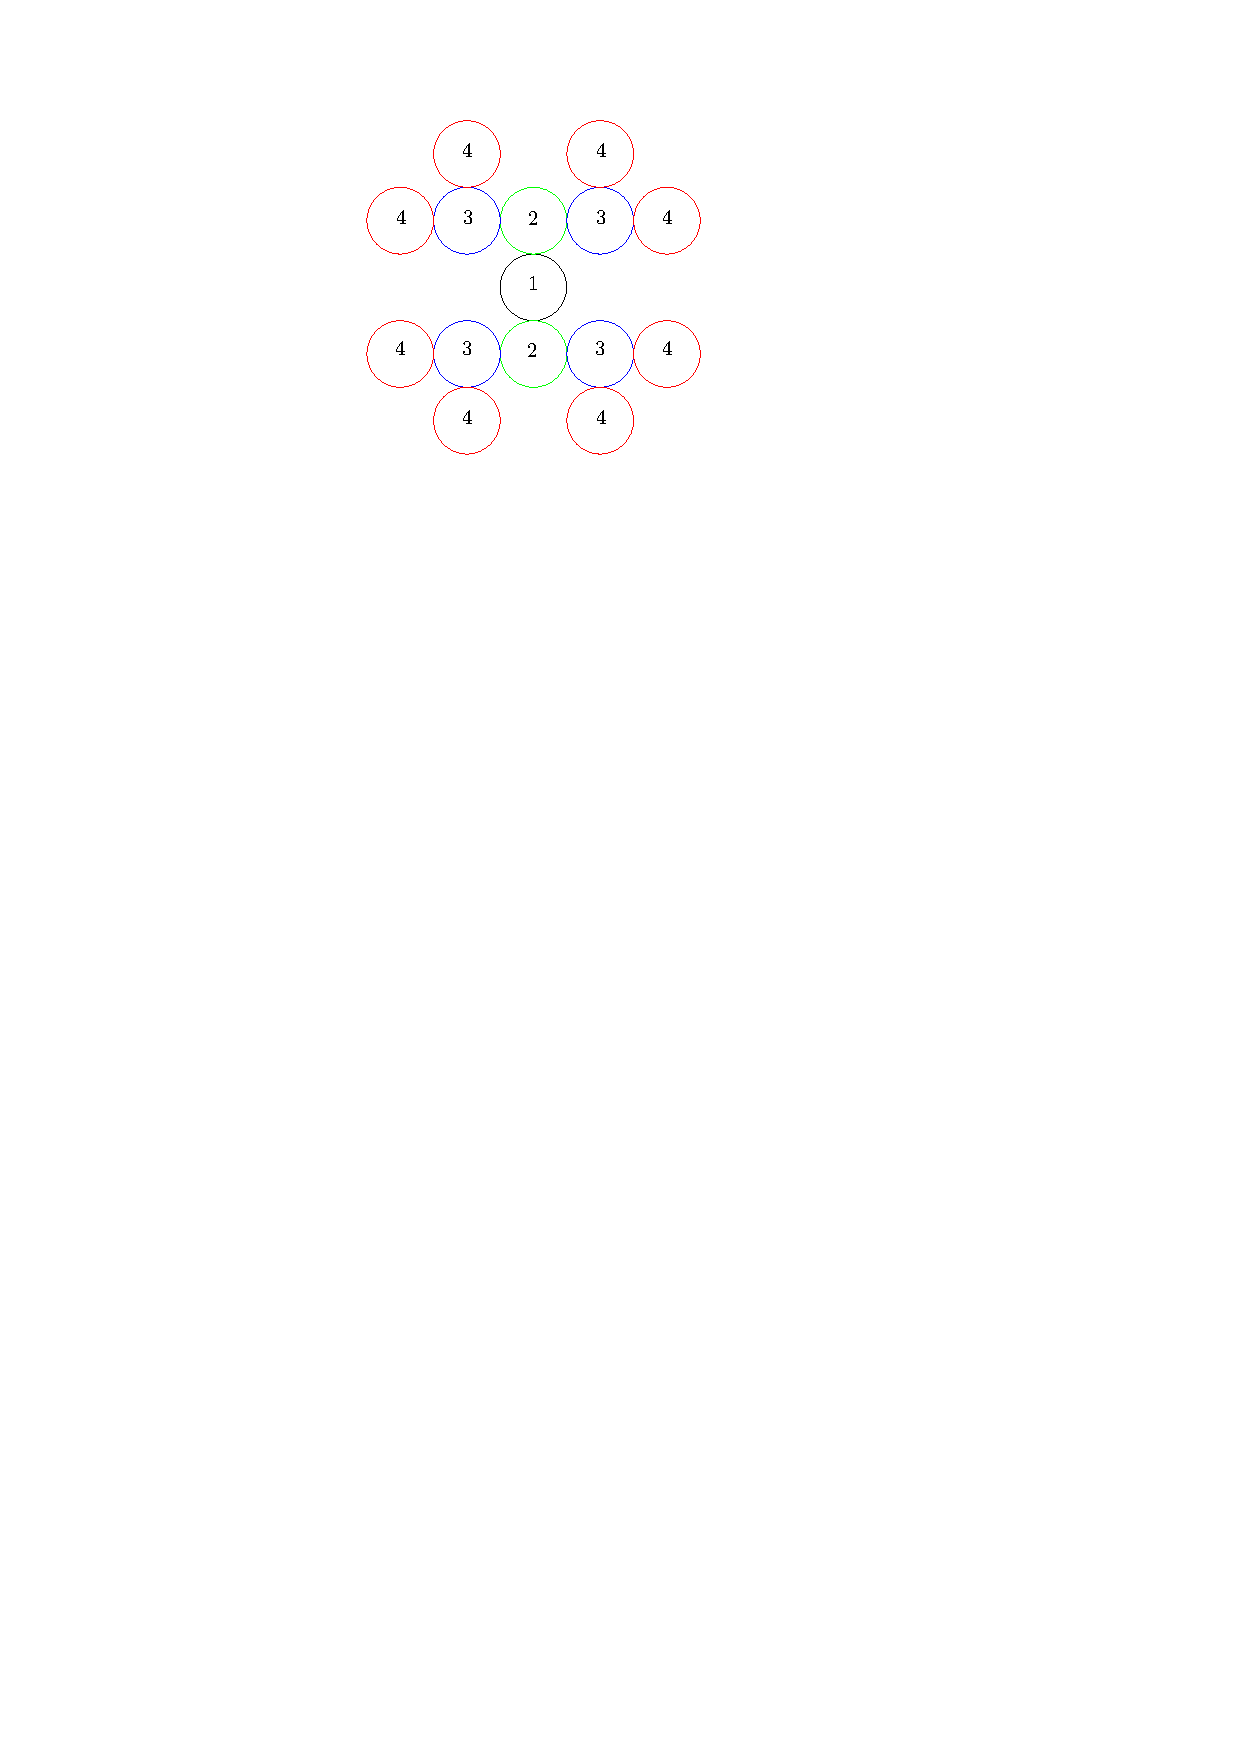
\includegraphics[width=\textwidth]{graphics/degree4arrangement.pdf}
	  \caption{A disk arrangement with four layers of disks}
	  \label{fig:circlePacking2-3}
  \end{subfigure}
  \begin{subfigure}[b]{0.24\textwidth}
	  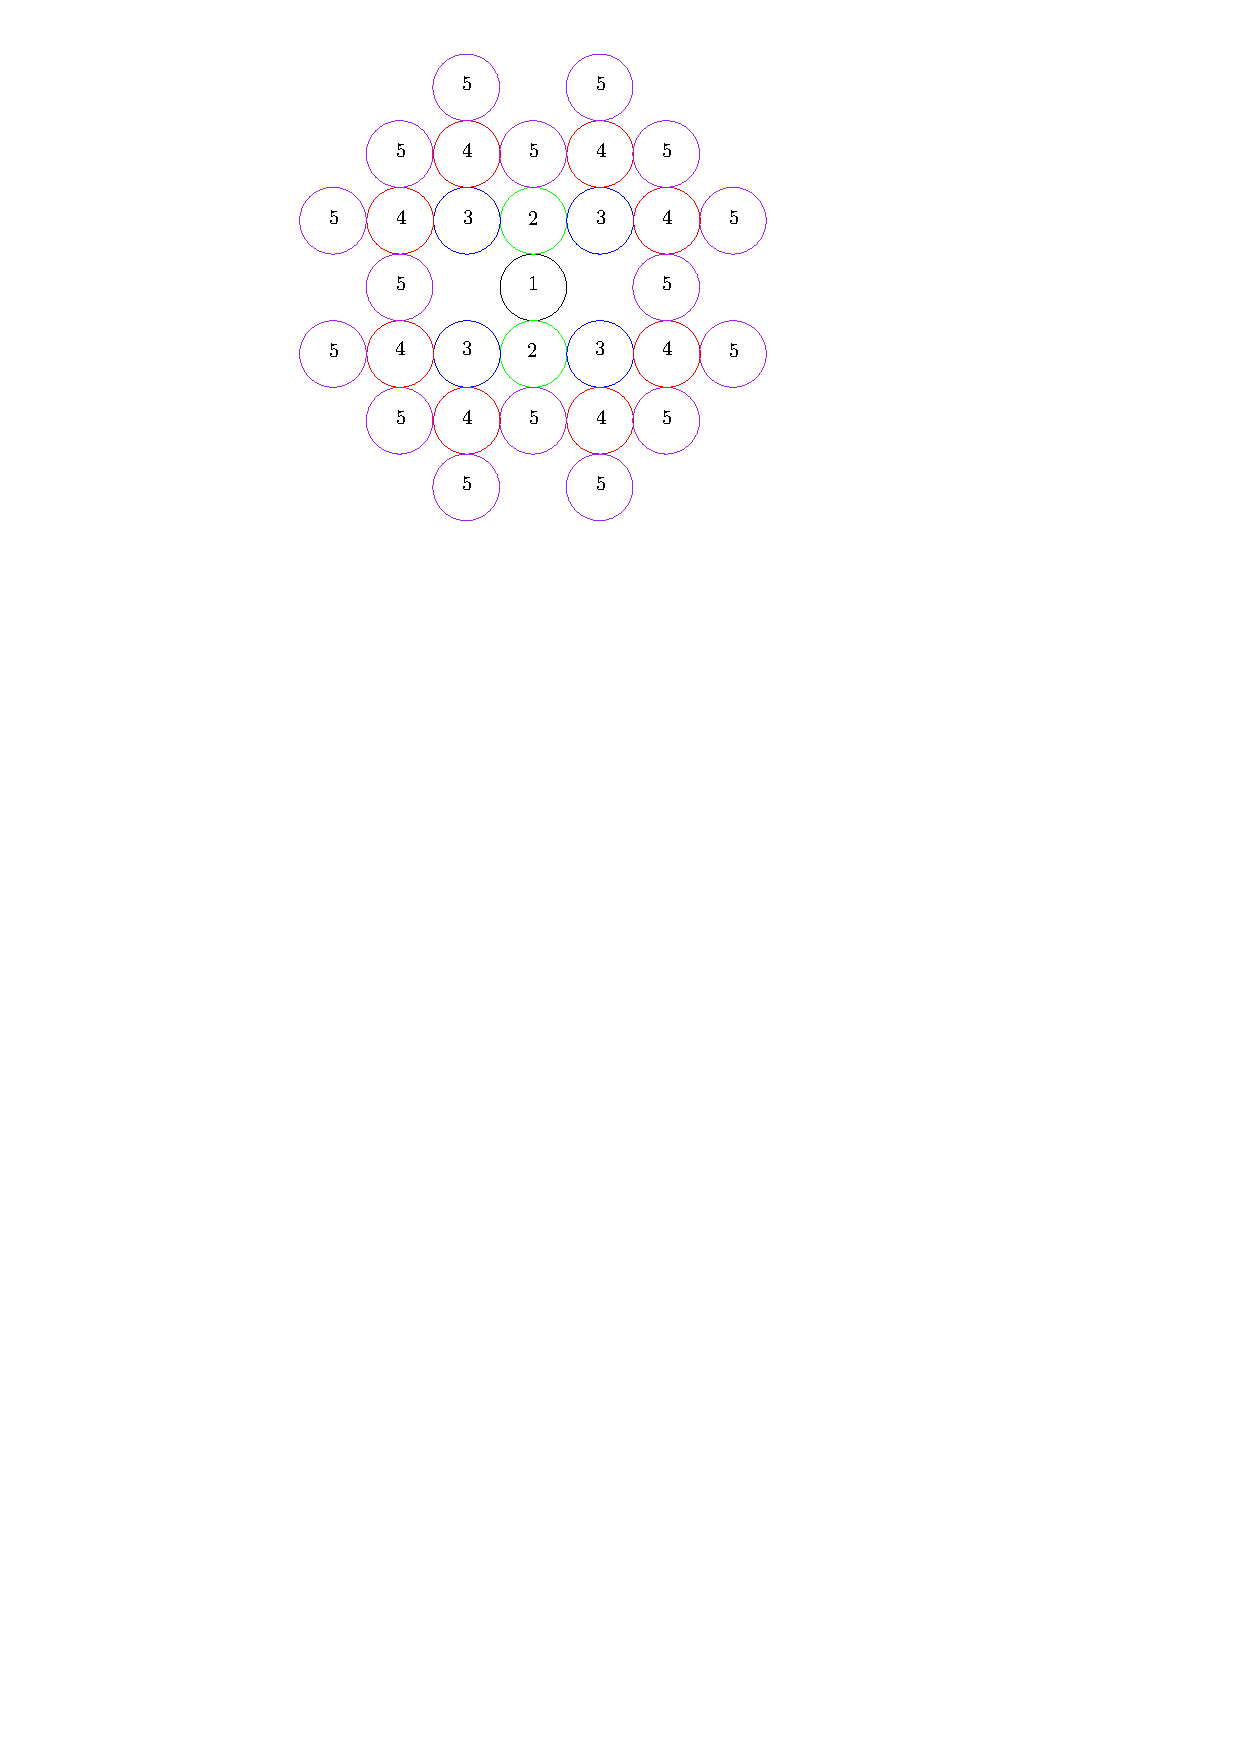
\includegraphics[width=\textwidth]{graphics/degree5arrangement.pdf}
	  \caption{A disk arrangement with five layers of disks}
	  \label{fig:circlePacking2-4}
  \end{subfigure}
\end{center} 
\caption{For $i=2,3,4,5$ the tree $T_i$ is a contact graph of unit disks.}
\end{figure}
% The first round has one unit disk.  
% The next round, two unit radii disk are in contact with the first, i.e. Figure \ref{fig:circlePacking1-1}.
% The subsequent rounds are shown in Figures \ref{fig:circlePacking1-2}, \ref{fig:circlePacking1-3}, and \ref{fig:circlePacking1-4}.  
% For each round $i$ we are adding $2^{(i-1)}$ disks, each with an area of $\pi$.  
% The area that the disk arrangement is bounded at round $i$ is a box of length $2\cdot (2\cdot (i-1)+1)$ totalling to an area of $(4\cdot i^2 - 4\cdot i + 1)$.  
% Meanwhile the total area of the disk arrangement at $i$ is $\pi \cdot (2^i - 1)$.  The exponential growth rate of the disk packing will exceed its bounded area for sufficiently large $i$, i.e. pick $i \geq 6$.
Figure \ref{fig:circlePacking-2} shows the first four non-trivial trees as a contact graph of unit disks.
Every disk at level up to $i$ is contained in a disk of radius $2\cdot i - 1$ centered at the origin.
The total area of the disk arrangement is $(2\cdot i -1)^2 \cdot \pi$. 
When $i\geq 8$ we have a contradiciton.%the total area of the disk arrangement exceeds the total bounded area and thus we have a contradiction.

\begin{figure}[!htbp]\label{fig:circlePacking-3}
\begin{center}
    %add desired spacing between images, e. g. ~, \quad, \qquad etc.
    %(or a blank line to force the subfigure onto a new line)
  \begin{subfigure}[b]{.48\textwidth}
  \begin{center}
	  \includegraphics[scale=.9]{graphics/OrderedDiskArrangementExample1.pdf}
	  \label{fig:circlePacking3-1}
	  \end{center}
  \end{subfigure}
  \begin{subfigure}[b]{0.48\textwidth}
  \begin{center}
	  \includegraphics[scale=.9]{graphics/OrderedDiskArrangementExample2.pdf}	  
	  \label{fig:circlePacking3-2}
	  \end{center}
  \end{subfigure}
  \caption{Consider these two ordered disk arrangements where A and B are in the concentric rings of disks.  The large disks are in contact to A and B respectively.  
  If A and B are adjacent, then there is a restriction of how large the size of the disks can be that are attached to them as seen in on the left.  
  Whereas if A and B are not adjacent in this disk arrangment as shown on the right, the size of the kissings disks could be arbitrarily large.}
\end{center} 
\end{figure}

There are instances where a planar graph with weights admits a realization but the cyclic order of neighbors may not be the same as the combinatorial embedding.
Define $G$ as follows: start with a star centered at $C$ and with 6 leafs, $A_1$ through $A_6$; attach two leafs, $B_1$ and $B_2$, to $A_1$ and  $A_2$ respectively (see  Figure \ref{fig:circlePacking-3}).
Let the weight of $C$ be $1+\epsilon$ for sufficiently small $\epsilon > 0$.
The neighbors of $C$ have unit weight.
The weights of the two leaves have weight $\frac{1}{\epsilon}$/
The right of Figure \ref{fig:circlePacking-3}) shows a realization where $A_1$ and $A_2$ are in opposite position of the counter-clockwise order around $C$.
If $A_1$ and $A_2$ are required to be consecutive in the counter-clockwise order around $C$, there is no realization.
%as epsilon goes to 0 the half planes approximates the disks and so the disks will intersect as well.  label everything, draw halff planes, epsilon and delta, 1/epsilon.

Suppose there is a realization where $A_1, \ldots, A_6$ are in the counter-clockwise order around $C$ (see Figure \ref{{fig:DiskArrangement-4}}).
If $\epsilon>0$ is sufficiently small, then the centers of of $A_1, \ldots, A_6$ are arbitrarily close to the vertices of a regular hexagon.
Consider the common tangent lines between $A_1$ and $B_1$ and $A_2$ and $B_2$.
The possible position of tangent line between $A_1$ and $B_1$ ranges from the common tangent line of $A_1$ and $A_6$ to the common tangent line of $A_1$ and $A_2$.
Similarly, The possible position of tangent line between $A_2$ and $B_2$ ranges from the common tangent line of $A_2$ and $A_3$ to the common tangent line of $A_1$ and $A_2$.
In any position, the common tangent lines between $A_1$ and $B_1$ and $A_2$ and $B_2$ intersect.
If $\frac{1}{\epsilon}$ is sufficiently large, then the disks $D_1$ and $D_2$ also intersect.
This contradicts that there is a realization.

\begin{minipage}{\linewidth}\begin{center}
\includegraphics[width=.4\columnwidth]{graphics/orderedPlaneIntersection.pdf}
\end{center}
\captionof{figure}{This example represents a disk arrangement and its contact graph.}
%Figure shows a 5-cycle with a unique realization of a disk arrangement.
\label{fig:DiskArrangement-4}
\end{minipage}

Figure \ref{fig:circlePacking-3} shows how an ordered contact graph may not be realizable.  
On the left, it shows a limitation on the weights of the disks that are in contact with disks A and B. 
On the right, the figure shows the order where A and B are on opposing ends of the ring of disks and can allow of arbitrary size of wieghted disks in contact with A and B.
% Figure \ref{fig:orderedFaces.pdf} shows three polygons with a common hinge.
% In the counter-clockwise order $(A,B,C)$, the polygonal linkage admits a realization whereas in the counter-clockwise order $(A,C,B)$, it does not admit a realization.
% \subsection{Disk Packing Confinement Problem}

% Given inputs of radii 
% By adding constraints to the embeddings of disk arrangements, we can devise realizability problem 
% by a volume argument.
% \begin{enumerate}%1,2,3,4....
% \item Round 1: Start with a disk of unit radius.
% \item Round 2: Add two kissing disks, each of diameter 2, that do not intersect with any other 
% disk (they 
% may kiss other
% disk).
% \item Round 3 and Higher: For each new kissing disk added, add two more non-intersecting kissing 
% disks of diameter 2 to it.
% \end{enumerate} 


% Figure (\ref{fig:circlePacking-1}) illustrates the iterative problem.  The problem with this is that 
% the area in
% which is necessary to contain this disk growing disk arrangement will exceed the area needed to 
% contain it.





%The corresponding intersection graph of a disk packing is a graph whose vertices are the disks and edges correspond to two disks that contact each other.
% \section{Disk Arrangements}
% It turns out the disk arrangements are an equivalent way to to represent plane graphs.  By 
% representing vertices as interioir disjoint disks and by representing edges as as points of 
% intersections (contact), \textit{kissing 
% points} between two disks.  The graph corresponding to a given disk arrangement, $\DD$, is said to 
% be the \textit{contact graph}. A \it{disk arrangement} is a set, $\DD$, of pairwise 
% interior-disjoint disks in the plane, 
% $\DD=\left\lbrace C_i \right\rbrace_{i = 1}^n $.
% $\left\lbrace C_i \right\rbrace_{i = 1}^n $ such that for any circle $C \in \left\lbrace C_i 
% \right\rbrace_{i = 1}^n$, $C$


% %(fig 1) a disk arrangement
% %(fig 2) an equivalent contact graph to (fig 1)
% A classical result by Thurston and Koebe is that every disk arrangement embedded into the plane had 
% a corresponding plane graph.
% \begin{thm}[\ref{stephenson2005introduction}Disk Packing Theorem]\label{thm2-1}
% For every graph $G$, there is a disk arrangement in the
% plane whose contact graph is isomorphic to $G$.
% \end{thm}

% %add a paragraph with atoms of molecules are modeled with disks and balls of fixed radii. The 
% %if two disks are in contact, then the  distance between their centers  = the sum of the radii
% %conclude: disk arrangements are better models for representing atoms and molecules fixed distance 
% % betweeen atoms
% \begin{prop}
%  For every linkage $L$, there is a disk arrangement in the
% plane whose contact graph is isomorphic to $L$.
% \end{prop}



% \begin{enumerate}%1,2,3,4....
% %\item Introduce the circle packing theorem.
% \item Show the relation between polygonal linkages and disk arrangengements.
% \end{enumerate} 
% % \subsubsection{Ordered Disk Arrangement}
% Suppose we're given a tree. By the disk packing theorem we can ascertain a sense of order for the 
% isomorphic disk packing.  An \textit{ordered disk arrangement} is a rooted tree in which the 
% counter-clockwise ordering of adjacent vertices.
% % 


% The embedding problems for trees and corresponding disk arrangements are as follows:
% \begin{prob}[Unordered Realizibility Problem for the Tree]\label{problem:UnorderedContactGraph}
% For a tree with positive weights for the verticies, it asks whether it is a contact graph of some 
% disk arrangement where the radii are equal to the vertex weights.
% \end{prob}

% \begin{prob}[Ordered Realizibility Problem for the Tree]\label{problem:OrderedContactGraph}
% For a tree with positive weights for the vertices, it asks whether its corresponding graph is the 
% ordered contact graph of some disk arrangement where the radii equal the vertex weights.
% \end{prob}
\section{Configuration Spaces}
\begin{quote}
Just as one can compose colors or forms, so one can compose motions.
\end{quote}
{\raggedright{}Alexander Calder, 1933}

Recall Figure \ref{fig:HingedHaberdasher} illustrating the hinged dissection that formed a square and triangle and several drawings of the hinged dissections that simulate the motion of moving the polygons around the hinge points to form each shape.  The set of all drawings in that motion represents the \textit{configuration space} for that polygonal linkage.  In this section we will formally describe the configuration space for each object we've drawn thus far.


% We'd like to describe motions and range of motions of embedded graphs, linkages, polygonal 
% linkages, and disk arrangements.  Table \ref{table:configurationSpace-1} provides the definition of 
% \textit{reconfiguration} for each type of object covered so far:
% \begin{center}
% \begin{table}[htbp!]
% \begin{tabular}{|p{.2\textwidth}|p{.79\textwidth}|}
% \hline
% Object Type&Definition of Reconfiguration\\\hline
% Graph Embeddings&a continuous motion of the vertices that never causes the edges to 
% intersect.\\\hline
% Linkage&a continuous motion of the vertices that preserves the lengths of the edges and never 
% causes 
% the edges to intersect.\\\hline
% Polygonal Linkage&a continuous motion of polygons that preserves shapes of polygons, hinge point 
% pairings, and never causes the polygonal sides to intersect.\\\hline
% Disk Arrangement&a continuous motion of disks that preserves disk radii, pairs of contact points, 
% and never causes disks to intersect.\\\hline
% \end{tabular}\label{table:configurationSpace-1}
% \end{table}
% \end{center}




% For graphs, a \textit{reconfiguration} is a continuous motion of 
% the vertices that preserve the length edges and never cause edges to collide \cite{AKR+04}.  For 
% polygonal linkages, a reconfiguration is 

\subsection{Configuration Spaces of Graph Drawings}
Recall that for a graph drawing we have an injective mapping $\Pi : V \mapsto \bbR^{2}$ which maps vertices to distinct points in the plane.  %and for each edge $\curlybraces{u,v} \in E$, a straight line segment, $c_{u,v}:[0,1]\mapsto \bbR^2$ such that $c_{u,v}(0) = \Pi(u)$ and $c_{u,v}(1) = \Pi(v)$, and does not pass through other vertices.
The mapping $\Pi$ uniquely determines each edge.
An edge $\curlybraces{u,v} \in E$, is mapped to a straight line segment, $c_{u,v}:[0,1]\mapsto \bbR^2$ such that $c_{u,v}(0) = \Pi(u)$ and $c_{u,v}(1) = \Pi(v)$, and does not pass through other vertices.
%For each vertex of $G$, the embedding of the vertex lies in the plane, i.e. $\Pi(v) \in \bbR^2$.  
Let $\DD_G$ be the set of all drawings of the graph $G$.  
By labelling the vertices of $G$, e.g. $v_1, v_2, \dots, v_k, \dots, v_{n}$, we can create a mapping from $\mu: \DD_G \mapsto \bbR^{2\vert V \vert}$ where the coordinates of $\Pi(v_k)$ are the $(2k)^\text{th}$ and $(2k+1)^\text{st}$ coordinates in $\bbR^{2\vert V \vert}$.  
$\mu(\Pi)$ is a configuration.
The configuration space is the set of $\mu(\Pi)$ for all drawings $\Pi$.  

\subsection{Configuration Spaces of Linkages}

Consider drawings of a graph that respects the length assignment.  
A \textit{realization} of a linkage, $(G,\ell)$, is a drawing of a graph, $\Pi$, such that for every edge $\{u,v\} \in E$, $\ell\left( \{u,v\} \right) = \left\vert \Pi(u) - \Pi(v) \right\vert = \left\vert \Pi(v) - \Pi(u) \right\vert$. 
A \textit{plane realization} is a plane drawing with the property, $\ell\left( \{u,v\} \right) = \left\vert \Pi(u) - \Pi(v) \right\vert$.
First let's define the space of realizations for a corresponding linkage, i.e.:
$$P_{(G,\ell)} = \set{\Pi\in \DD_G }{\forall \{u,v\} \in E\text{, }\ell\left( \{u,v\} \right) = \left\vert \Pi(u) - \Pi(v) \right\vert}$$
With respect to $P_{(G,\ell)}$, we can establish a configuration space that allows one to study problems of motion.  
For each vertex of $G$, the drawing of the vertex lies in the plane, i.e. $\Pi(v) \in \bbR^2$.  
By enumerating each vertex of $G$, e.g. $v_1, v_2, \dots, v_k, \dots, v_{n}$, we can create a mapping from $\mu: P_{(G,\ell)} \mapsto \bbR^{2\vert V \vert}$ where the corresponding coordinates of $\Pi(v_k)$ are in the $(2k)^\text{th}$ and $(2k+1)^{st}$ coordinates in $\bbR^{2\vert V \vert}$.  
The configuration space is $\mu\lr{P_{(G,\ell)}}$.  

Using standard definitions from real analysis, we can begin to pose problems about linkages with respect to a corresponding configuration space.  
A continuous function $\gamma: [0,1]\mapsto \mu\lr{P_{(G,\ell)}}$ is a path from a realization $\gamma(0)$ to another realization $\gamma(1)$.
$\gamma$ can be thought of as an animation of drawings that starts at $\gamma(0)$ and ends at $\gamma(1)$.
%corresponds to the mapping of a realization of a linkage $\Pi_0$ and $\gamma(1)$ corresponds to another realization of a linkage $\Pi_1$.  
%If for any two elements $a,b \in \mu(P)$ that there exists a continuous path $\gamma$ such that $\gamma(0)=a$ and $\gamma(1)=b$, $\mu(P)$ is said to be path connected.   
%For $\gamma$ to be continuous we would have that for every $\epsilon > 0$, there exists a $\delta >0$ such that if $x,y \in [0,1]$ and $\vert x-y \vert <\delta$ then $\vlr{\vlr{\gamma(x)-\gamma(y)}}<\epsilon$.
Any two realizations in the same path-connected component can be animated from one to the other continuously.
The Carpenter's Rule states that every realization of a path linkage can be continuously moved (without self-intersection) to any other realization \cite{CDR03,Str05}.
To ask if $\mu\lr{P_{(G,\ell)}}$ is a connected space, is to ask if $\mu(P)$ is connected in $\bbR^{2\vert V \vert}$.
In other words, the realization space of such a linkage is always path-connected.

% \subsection{Configuration Spaces of Linkages}

% \textbf{NOTE THAT THIS SUBSECTION MAY HAVE REPEATED CONTENT}

% Let's focus on the space of embeddings of a linkage. If there are $n$ vertices of a linkage, 
% the \textit{configuration space} of a linkage is said to be a vector space of dimension $2 \cdot n$ 
% where edge length is preserved.  

% A \textit{configuration space} for a linkage $G$ and corresponding proper embedding, $L_1$ is said 
% to be for any other proper embedding of a linkage $G$, $L_2$, such that the lengths 
% of every edge of $G$ is preserved between the two embeddings, i.e.: 
% $$l\left( \left(u,v\right) 
% \right) = \left\vert 
% L_1(u) - L_1(v) \right\vert = \left\vert L_2(u) - L_2(v) \right\vert$$
% Equivalent embeddings include translations and rotations about the center of mass on $L(V)$.  We 
% further our embeddings by requiring that one vertice is pinned to the point of origin on the plane 
% as well as a neighboring vertex.


% Can a simple planar polygon be moved continuously to a position where all its vertices are in convex position, so that the edge lengths and simplicity are preserved along the way?

\begin{figure}[!htbp]%blah
\begin{center}
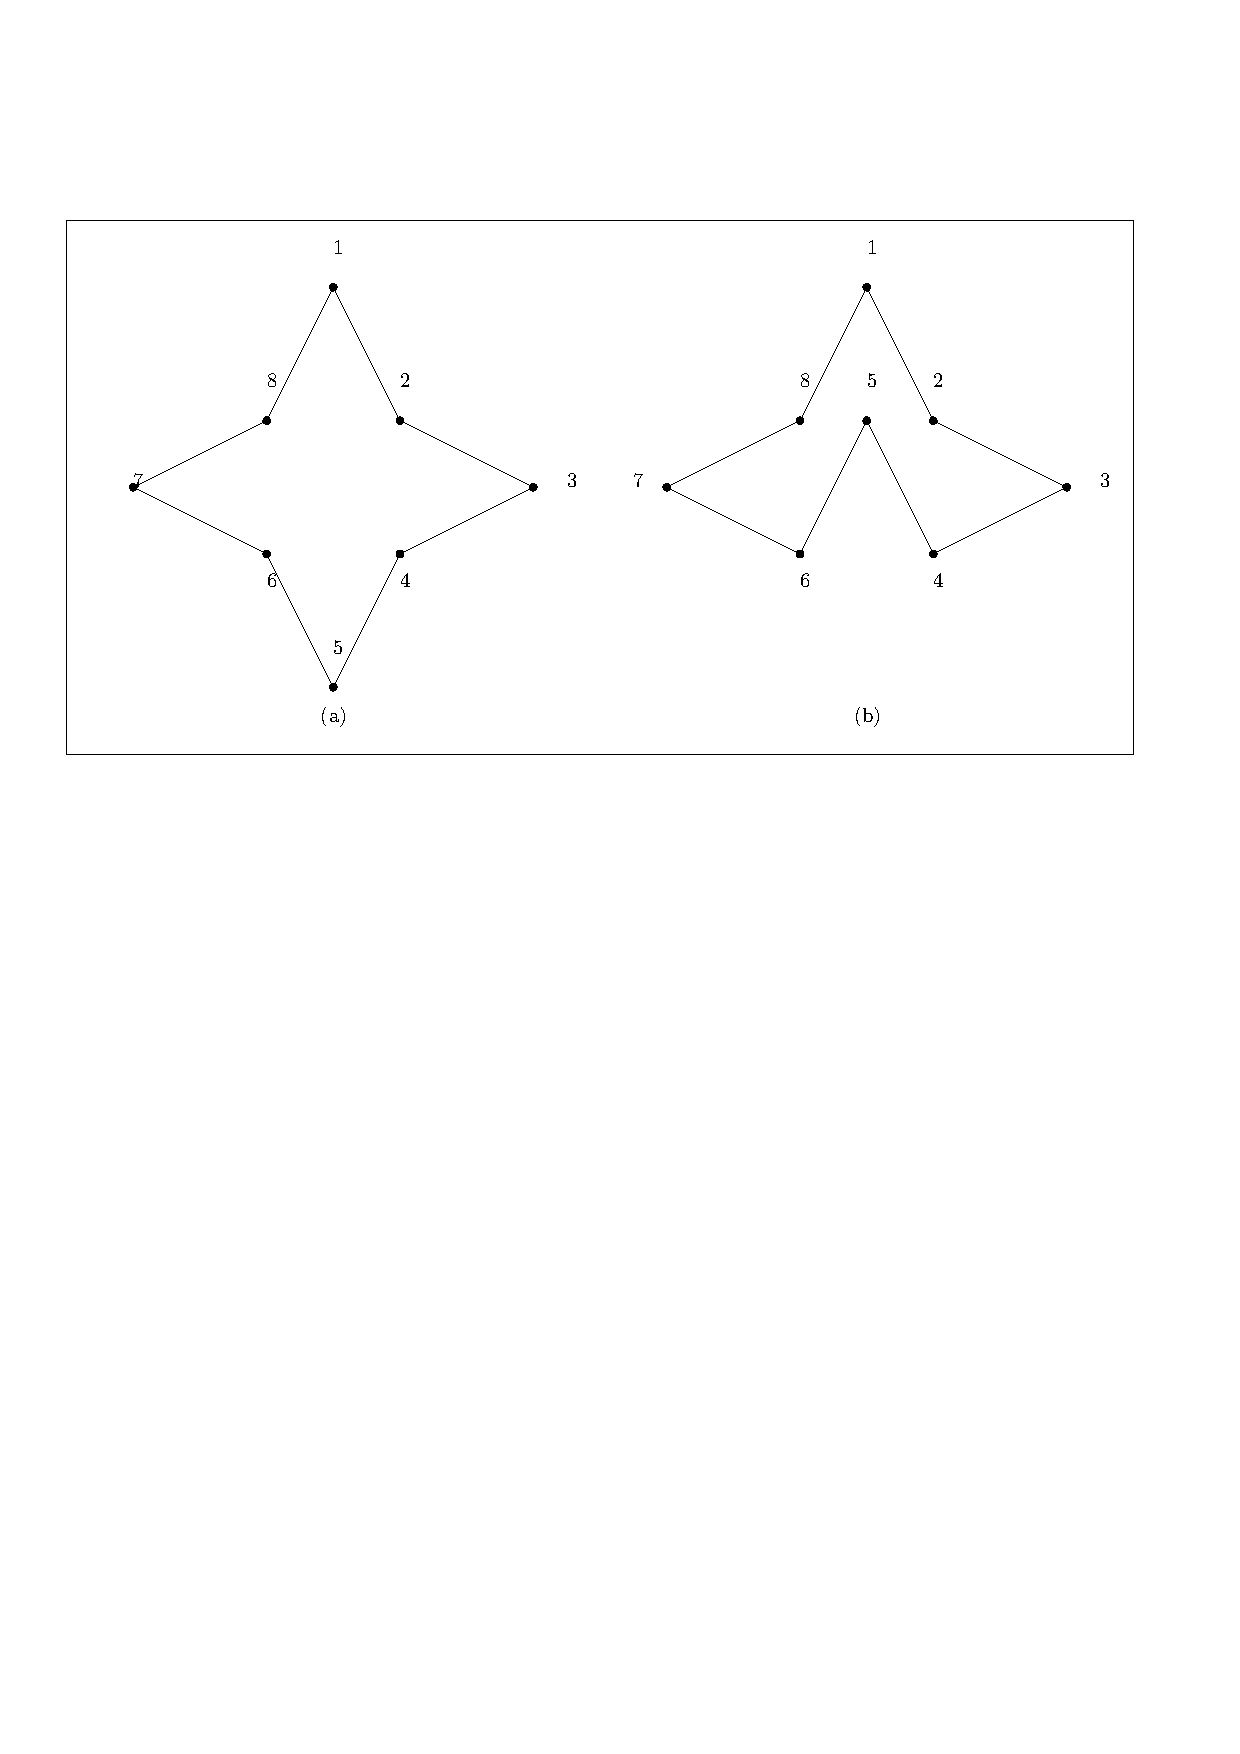
\includegraphics{graphics/twoEmbeddingsOfSameLinkage.pdf}
\end{center} 
\caption{(a) and (b) show a linkage in two embeddings.  Any realization of a path can be continuously moved without self-intersection to any other realizations.}
\label{fig:twoEmbeddingsOfSameLinkage.pdf}
\end{figure}

\subsection{Configuration Spaces of Polygonal Linkages}
The placement of a polygon is described by an isometry of Euclidian plane.
An isometry is a composition of a translation, a rotation, and a possible reflection.
As such, the isometry can be descibed as three parameters: $\lr{a,b,\theta}$ where $(a,b)$ is a translation vector; if $\theta \geq 0$, it describes a counter-clockwise rotation by $\theta$ and if $\theta < 0$, it descibes a reflection in the x-axis followed by a counter-clockwise rotation $\theta$.
For $m$ polygons there will be $3 m$ parameters.
Recall a realization of a polygonal linkage is an interior-disjoint placement of congruent copies of the polygons in $\PP$ such that the copies of a hinge are mapped to the same point (e.g., Figure \ref{fig:linkage-1}).
First consider the set of all realizations for the polygonal linkage $\left(\PP,\HH\right)$ and call it $P$.  
$\mu:P \mapsto \bbR^{3m}$ where $m$ is the number of polygons in $\PP$ is the configuration space function and the configuration space is the set $\mu(P)$. 

 \subsection{Configuration Spaces of Disk Arrangements}
rewrite where theta is not needed.  disks are symmetric and rotation does not help.
The placement of a polygon is described by an isometry of Euclidian plane.
An isometry is a composition of a translation, a rotation, and a possible reflection.
As such, the isometry can be descibed as three parameters: $\lr{a,b,\theta}$ where $(a,b)$ is a translation vector; if $\theta \geq 0$, it describes a counter-clockwise rotation by $\theta$ and if $\theta < 0$, it descibes a reflection in the x-axis followed by a counter-clockwise rotation $\theta$.
For $m$ polygons there will be $3 m$ parameters.
Recall a realization of a polygonal linkage is an interior-disjoint placement of congruent copies of the polygons in $\PP$ such that the copies of a contact are mapped to the same point (e.g., Figure \ref{fig:linkage-1}).
First consider the set of all realizations for the polygonal linkage $\left(\PP,\HH\right)$ and call it $P$.  
$\mu:P \mapsto \bbR^{3m}$ where $m$ is the number of polygons in $\PP$ is the configuration space function and the configuration space is the set $\mu(P)$. 

\begin{figure}[!htbp]
\begin{center}
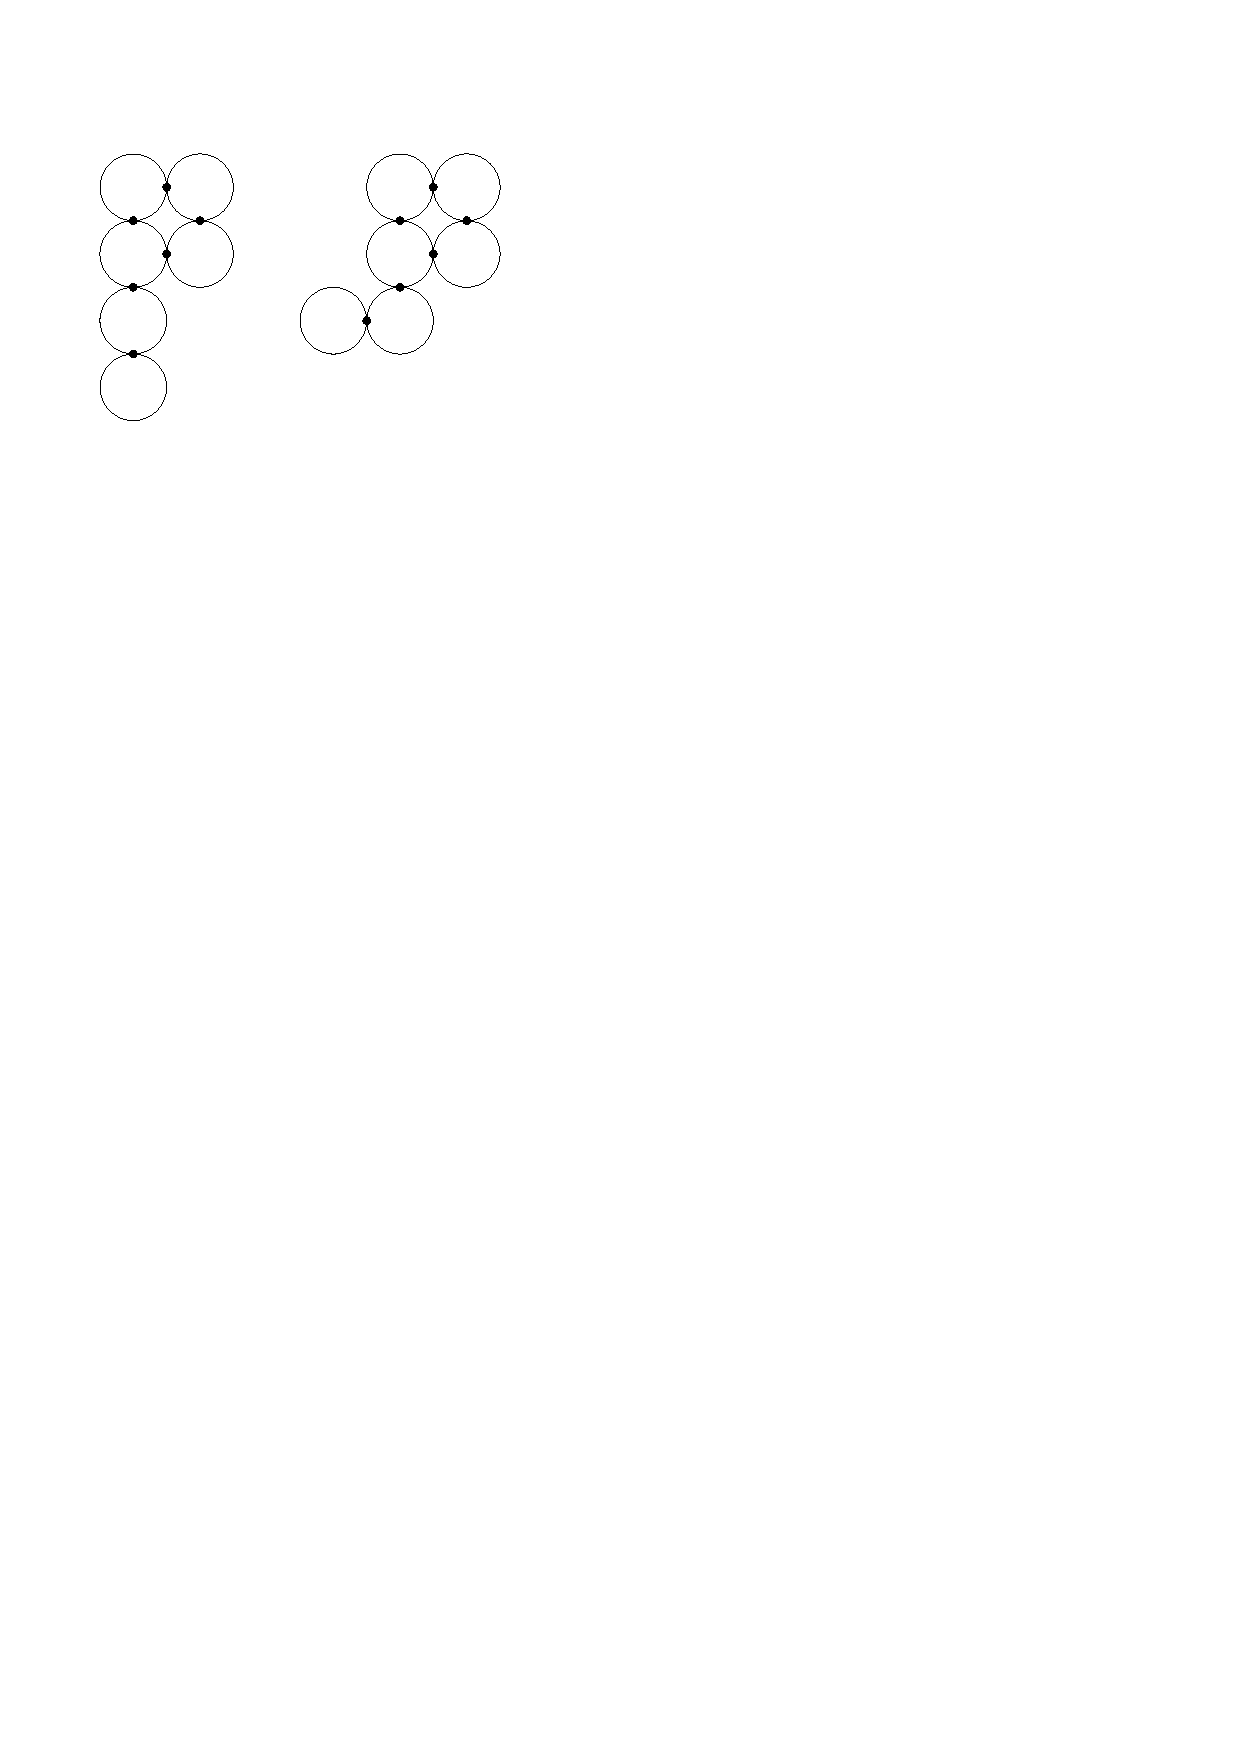
\includegraphics[scale=.75]{graphics/DiskPackingReconfiguration.pdf}
\end{center} 
\caption{An example of a disk arrangement where $A$ and $B$ have a large range of freedom to move around.  $C$, $D$, $E$, and $F$ are limited in their range of motion to due to their contact points.}
\label{fig:configuration-5}
\end{figure}

Consider the set of realizations $P$ for a given disk arrangement $\DD = \left\lbrace D_i \right\rbrace_{i=1}^n$.  For any realization $R \in P$, there exists a corresponding contact graph, $C$.  The configuration spaces of $\DD$ are sets of $R \in P$ that are classified by the equivalent contact graphs, i.e. if $R_1$, $R_2 \in P$ and their corresponding contact graphs $C_1$ and $C_2$ have a graph isomorphism, $\phi$, then $R_1$ and $R_2$ belong to the same configuration space.





% \subsection{Reconfiguration}



% We'd like to describe motions and range of motions of embedded graphs, linkages, polygonal 
% linkages, and disk arrangements.  Table \ref{table:configurationSpace-1} provides the definition of 
% \textit{reconfiguration} for each type of object covered so far:
% \begin{center}
% \begin{table}[htbp!]\label{table:configurationSpace-1}
% \begin{tabular}{|p{.2\textwidth}|p{.79\textwidth}|}
% \hline
% Object Type&Definition of Reconfiguration\\\hline
% Graph Embeddings&a continuous motion of the realized vertices that never causes the edges to 
% intersect.\\\hline
% Linkage&a continuous motion of the realized vertices that preserves the lengths of the edges and never 
% causes 
% the edges to intersect.\\\hline
% Polygonal Linkage&a continuous motion of polygons that preserves shapes of polygons, hinge point 
% pairings, and never causes the polygonal sides to intersect.\\\hline
% Disk Arrangement&a continuous motion of disks that preserves disk radii, pairs of contact points, 
% and never causes disks to intersect.\\\hline
% \end{tabular}
% \end{table}
% \end{center}








% 
% \paragraph{Confining Linkages to a Restricted Space Within a Configuration Space}
% So we've covered the idea of linkages within a plane; now let's constrain the plane to a strip and 
% have a linkage that is a \textit{polygon}, i.e. a linkage that forms a closed chain (e.g. Table 
% \ref{table:linkage-1}), hugging the boundaries of the strip:
% \begin{figure}[h]
% \begin{center}
%   ~ %add desired spacing between images, e. g. ~, \quad, \qquad etc.
%     %(or a blank line to force the subfigure onto a new line)
%   \begin{subfigure}[b]{0.49\textwidth}
% 	  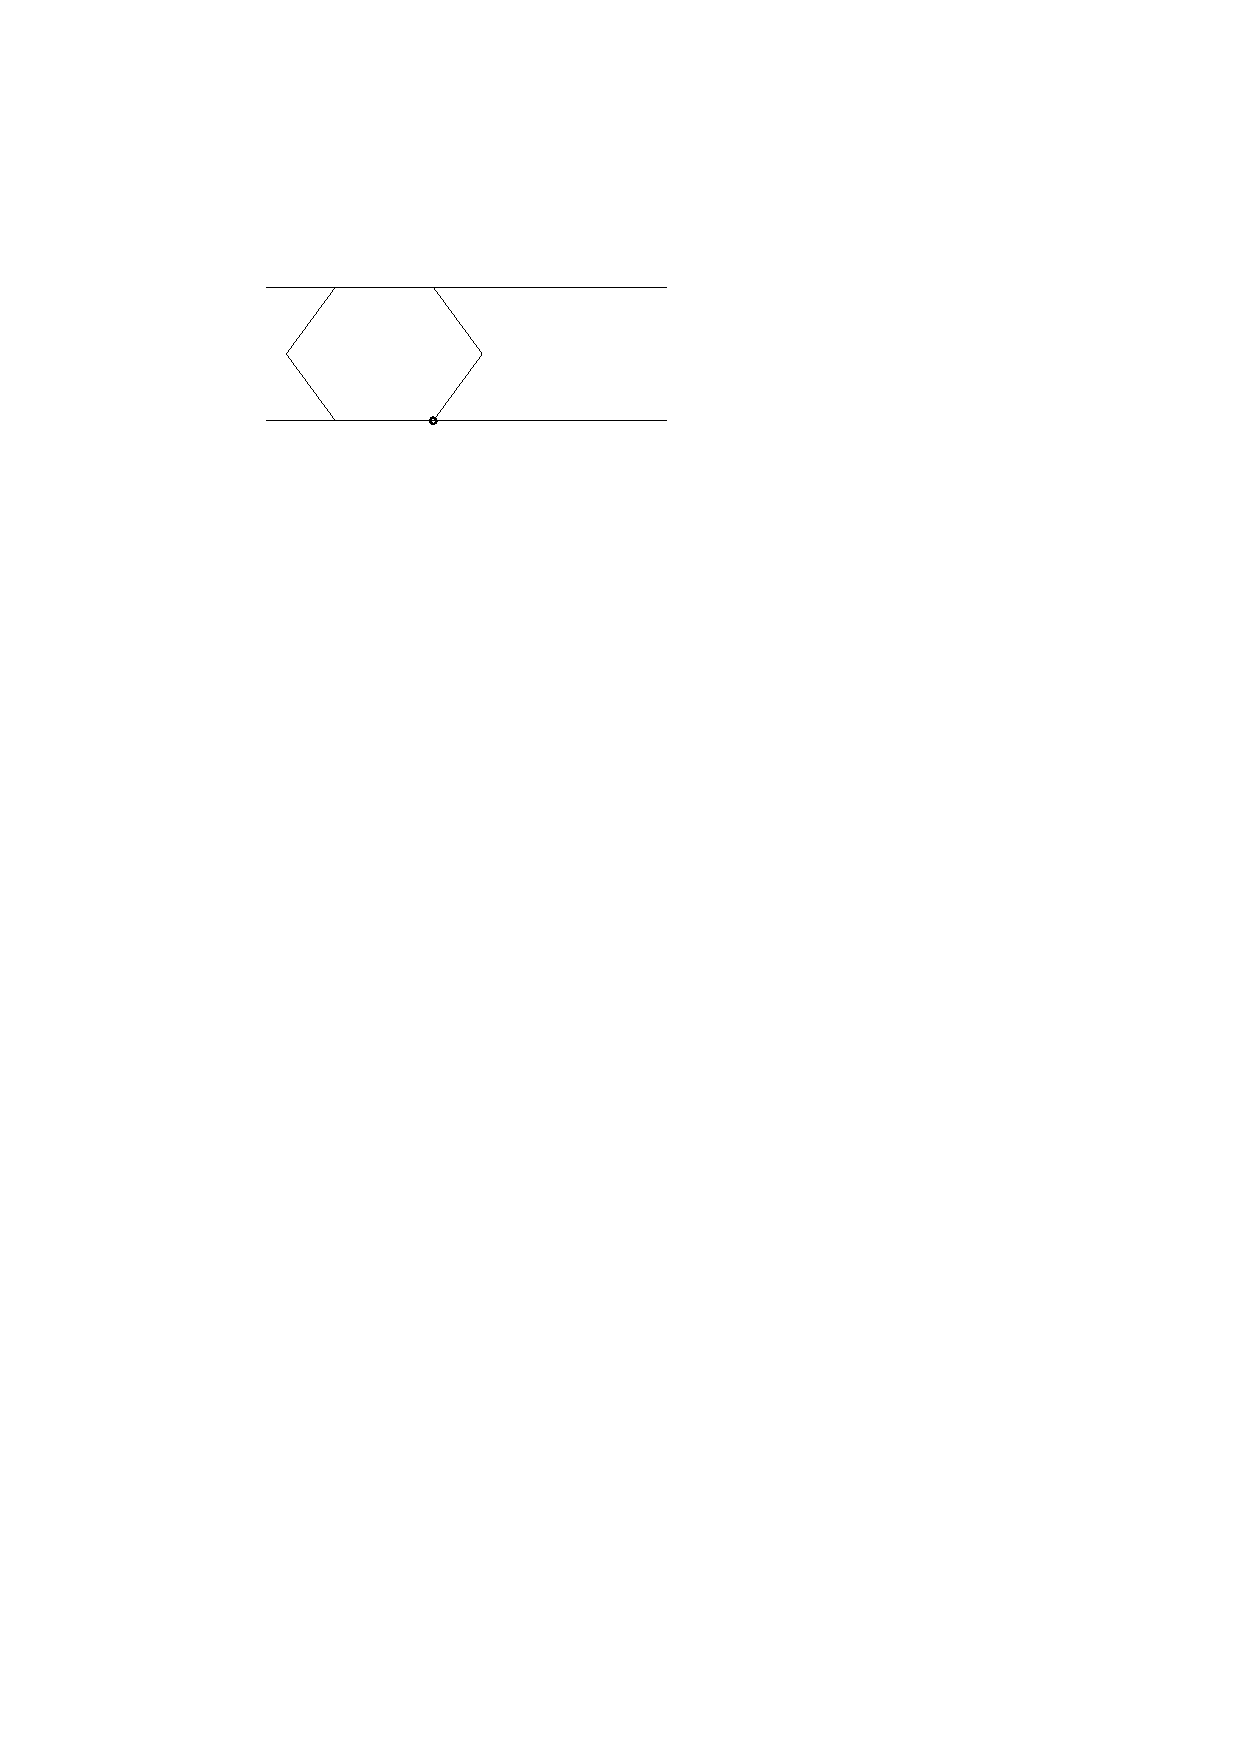
\includegraphics[width=\textwidth]{graphics/hexagonInChannelWithPinnedJointRight.pdf}
% 	  \caption{A bounded hexagon that resides in a channel with a pinned vertex}
% 	  \label{fig:linkage-1-1}
%   \end{subfigure}
%   \begin{subfigure}[b]{0.49\textwidth}
% 	  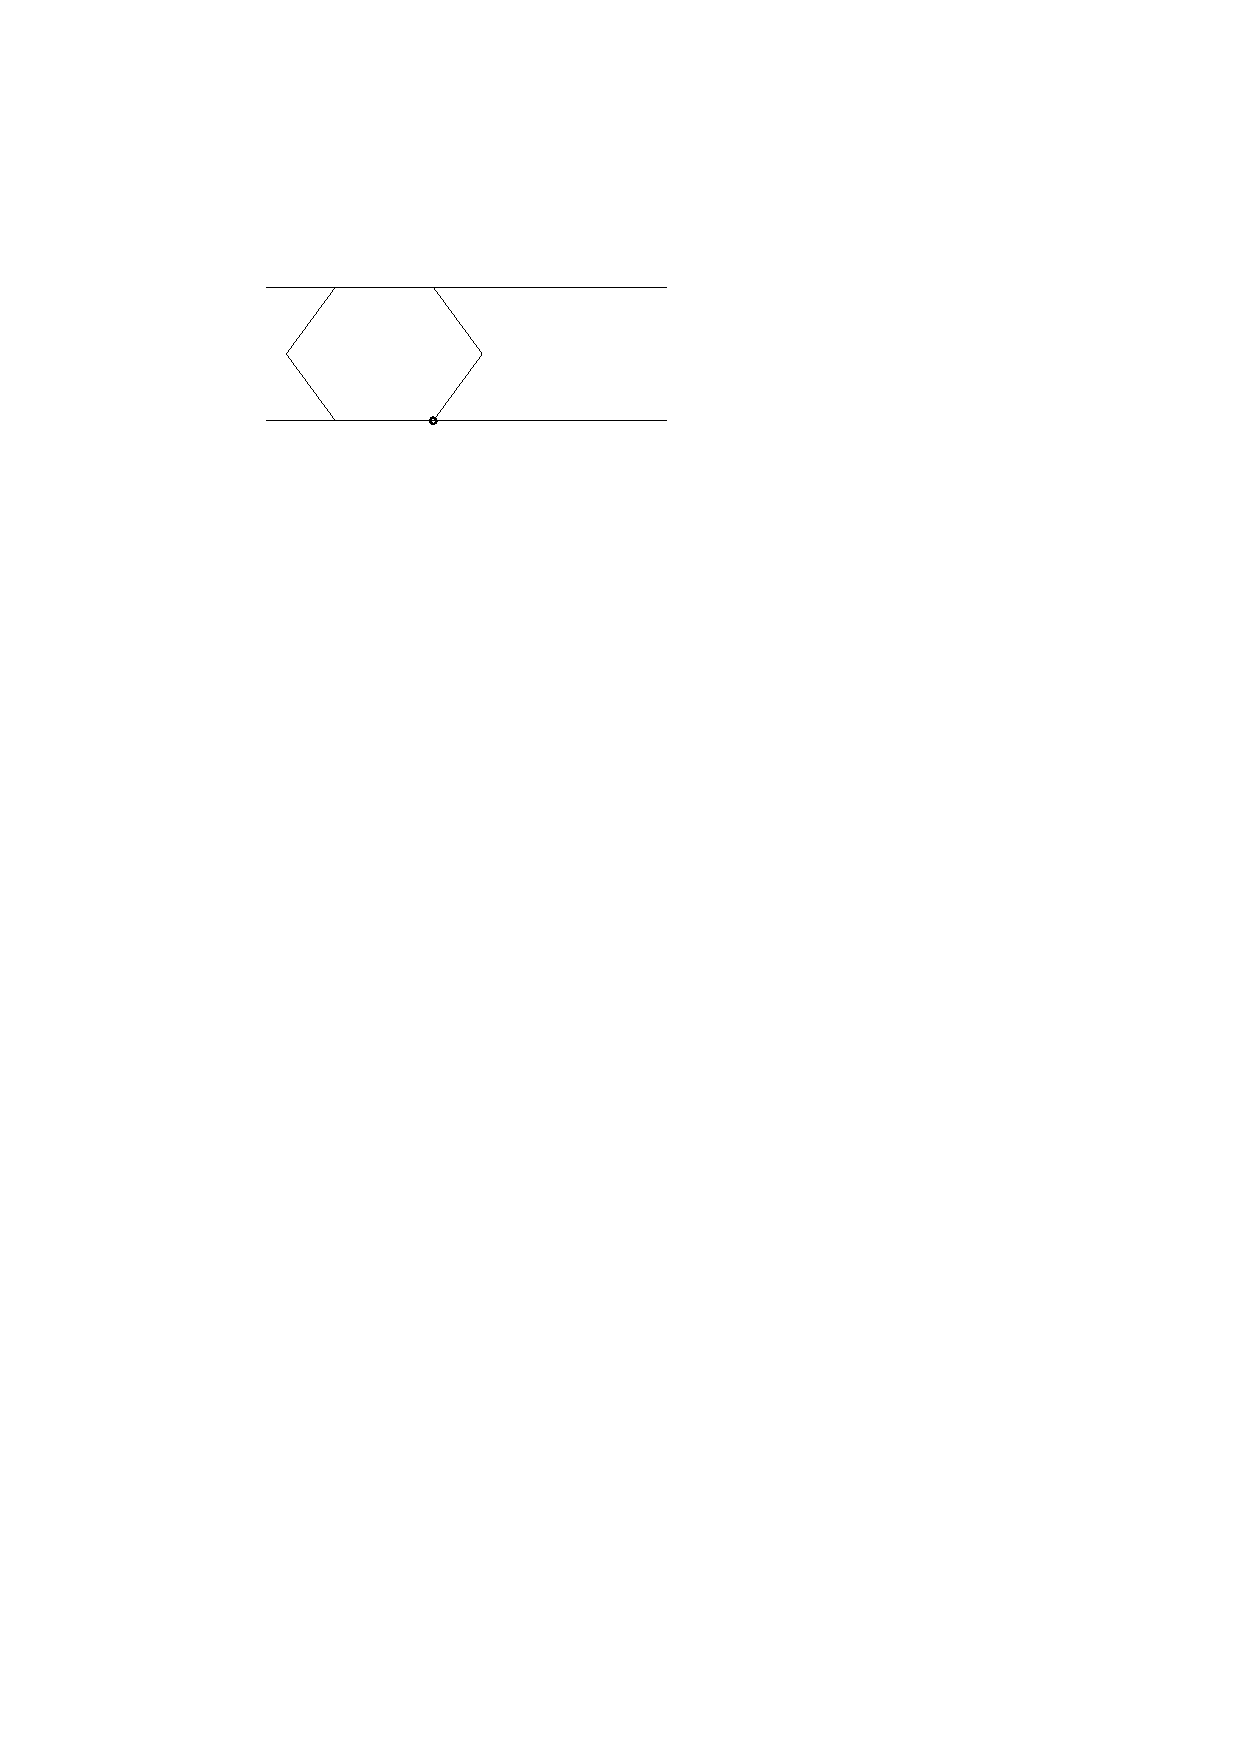
\includegraphics[width=\textwidth]{graphics/hexagonInChannelWithPinnedJointLeft.pdf}
% 	  \caption{The second realization of the hexagon residing in a channel with a pinned 
% vertex.}
% 	  \label{fig:linkage-1-2}
%   \end{subfigure}
% \end{center} 
% \caption{Due to the strip in the plane that the hexagon is bounded within the configuration space is 
% limited to just two realizations.}\label{fig:linkage-1}
% \end{figure}
% So here we have a linkage whose conifguration space is limited to just two realizations.  With just 
% two realizations, we can assign a binary value to them and have the linkage act as a boolean 
% variable.  We will revisit this concept when we cover satisfiability problems later on in the paper.
% \begin{figure}[h]
% \begin{center}
%   ~ %add desired spacing between images, e. g. ~, \quad, \qquad etc.
%     %(or a blank line to force the subfigure onto a new line)
%   \begin{subfigure}[b]{0.49\textwidth}
% 	  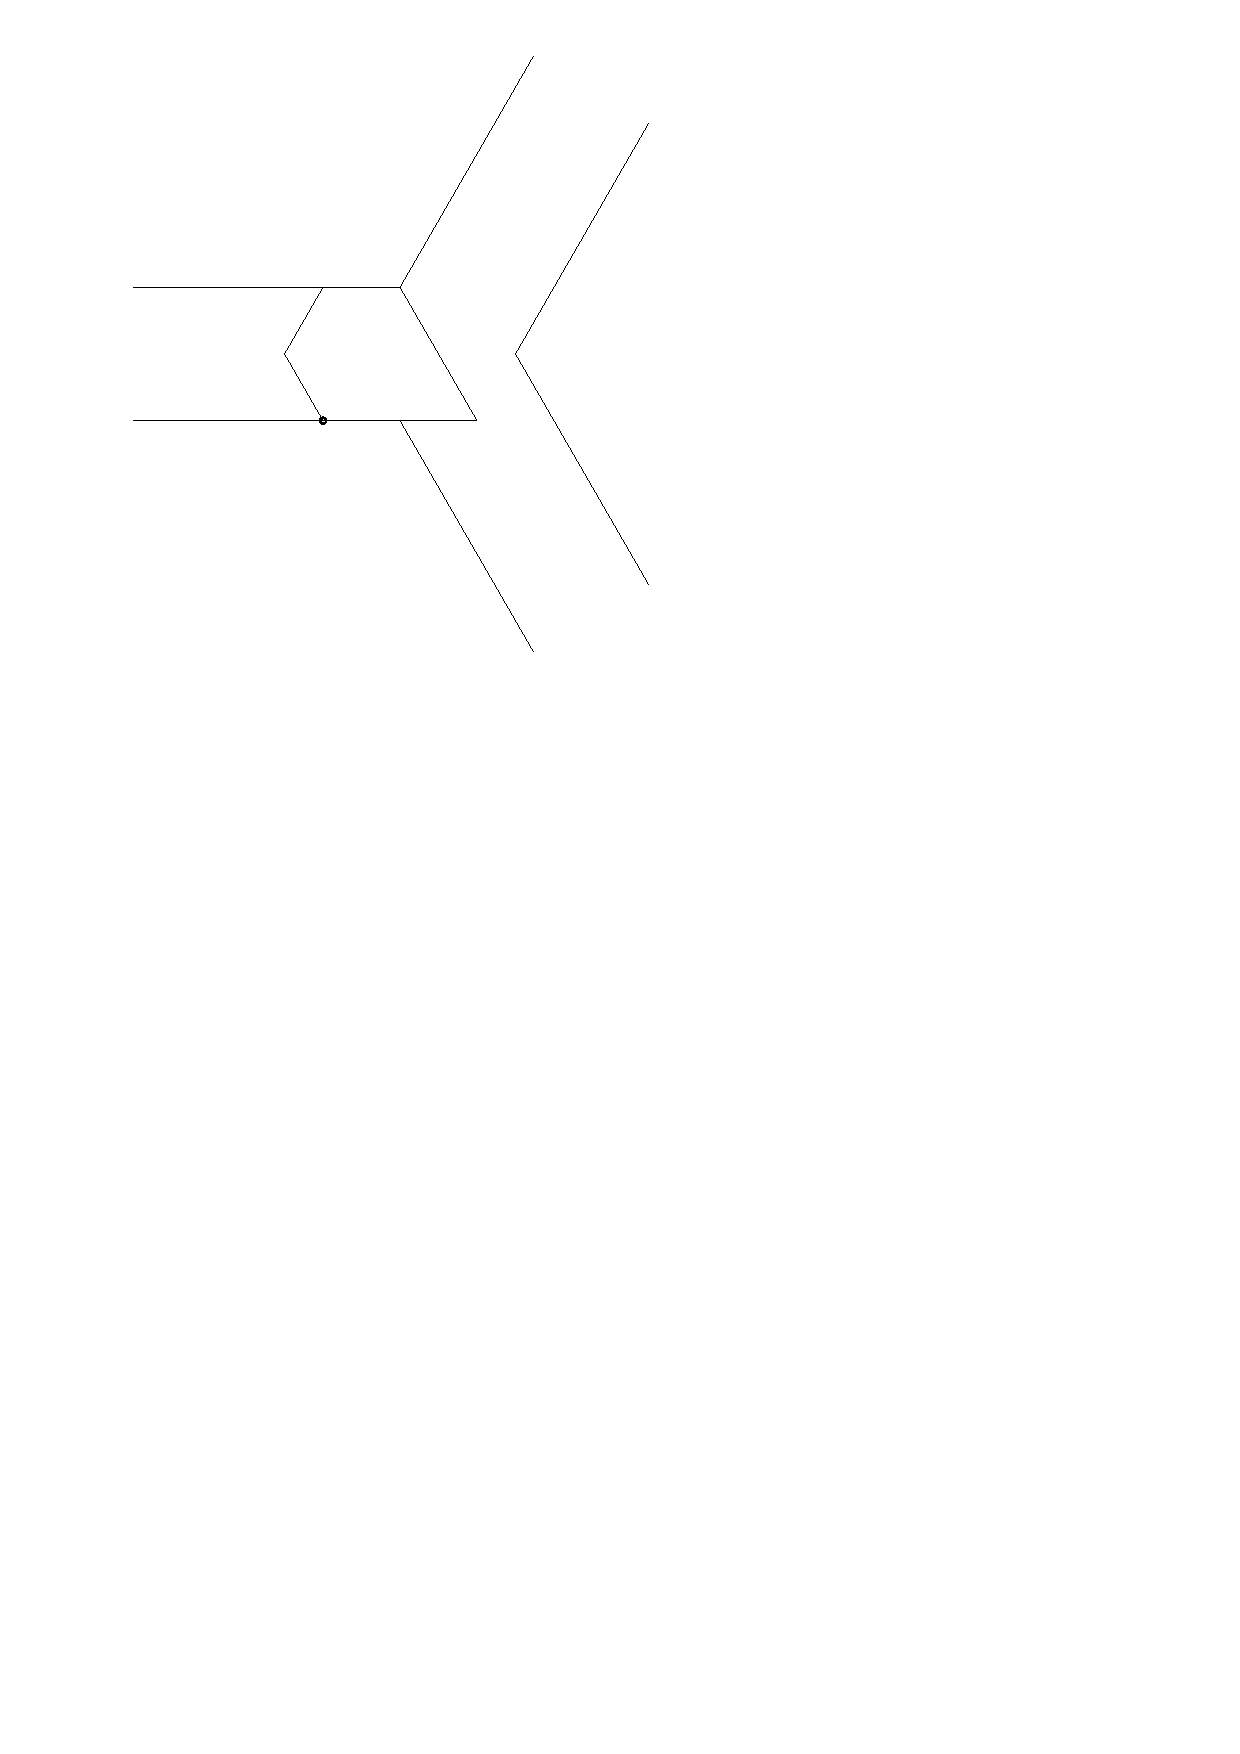
\includegraphics[width=\textwidth]{graphics/switchTerminalFinalized2.pdf}
% 	  \caption{A pentagon that is pinned in a channel junction that is formed by the sides of 3 
% large regular hexagons. It has two possible configurations, much like that of \ref{fig:linkage-1}}
% 	  \label{fig:linkage-2-1}
%   \end{subfigure}
%   \begin{subfigure}[b]{0.49\textwidth}
% 	  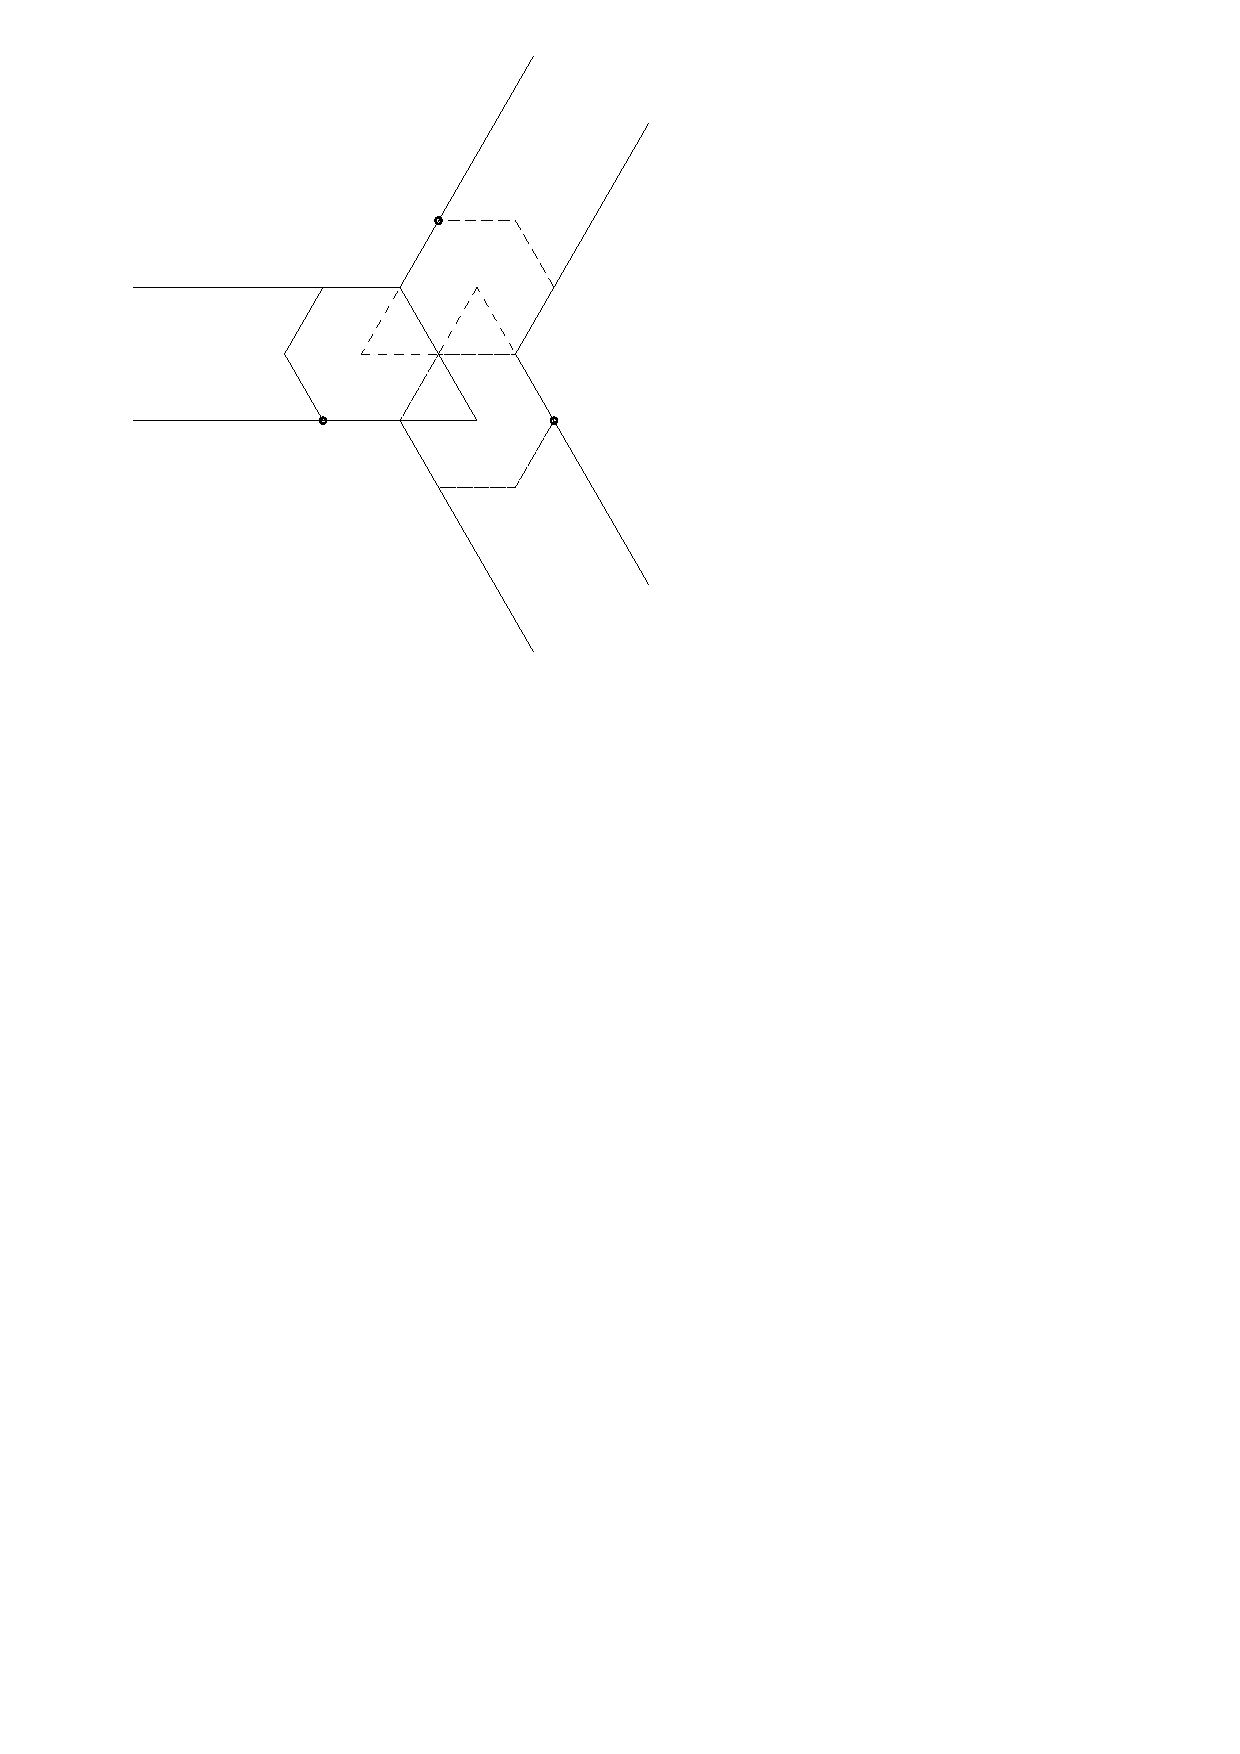
\includegraphics[width=\textwidth]{graphics/switchTerminalFinalized3.pdf}
% 	  \caption{A pinned pentagon residing in a channel junction that is formed by the sides of 
% 3 large regular hexagons with 2 dashed pentagons intersecting it.}
% 	  \label{fig:linkage-2-2}
%   \end{subfigure}
% \caption{Suppose the channel formed is a junction of three regular hexagons.  The polygon partially 
% residing in the junction is a regular hexagon with an equalateral triangle appended at an edge.  
% This polygon would prevent other polygons (i.e. the dashed polygons) of the same shape residing in 
% the center of the channel without intersection. This demonstrates that a the configuration space 
% within a multichannel environment can have concurrency issues, i.e. some configurations cannot be 
% realizable.}
% \end{center} \label{fig:linkage-2}
% \end{figure}\newpage
% Expanding upon the idea of \ref{fig:linkage-1}, forming channels with junctions as shown in Figure 
% \ref{fig:linkage-2} can be formed as such by evenly spacing the edges of a hexagonal lattice.  
% Visually, it is shown that only one of three possible pentagons can reside in the channel at one 
% time.  By asserting certain conditions on the lattice, and extending the problem to a greater 
% region 
% of a hexagonal lattice, we will be able to pose a realizability problem of whether a configuration 
% $\mathcal{A}$ can be reconfigured to $\mathcal{B}$ by switching pentagons without violating 
% overlapped polygon conditions.
% %Radius of regular polygons 
% %\newdimen\R
% %\R=3cm
% % \begin{figure}[h] 
% % \begin{center}
% % \begin{tikzpicture}
% % \begin{scope}
% % \filldraw[pattern=hexagons]  (0:\R) \foreach \x in {60,120,...,359} {
% %                 -- (\x:\R)
% %             }-- cycle (90:\R);
% % \end{scope}
% % \end{tikzpicture}
% % \caption{A hexagonal lattice contained in a hexagon.}
% % \label{fig:lattice}
% % \end{center}
% % \end{figure}
% %\newpage
% 
% % \begin{definition}[Graph]\label{def:linkages-2}
% % An ordered pair $G = (V, E)$ comprising a set $V$ of vertices or nodes together with a set $E$ of 
% edges or lines
% % \end{definition} 
% % \begin{definition}[Linkage]\label{def:linkages-1}
% % A collection of fixed-length 1D segments joined at their endpoints to form a graph.
% % \end{definition} 
% % A linkage can be thought of as a type of path-connected graph, i.e. the segments of a linkage are 
% the edges of a graph, and the endpoints of the segments are the vertices. For this paper, we 
% restrict our self to linkages that are simple planar graphs, i.e. a linkage that:
% % \begin{itemize}
% % \item[\rn{1}] does not have multiple edges between any pair of vertices,
% % \item[\rn{2}] does not have edges that cross, or
% % \item[\rn{3}] have loops (i.e. $(v,v) \in E$).
% % \end{itemize}  
% % \begin{definition}[Cycle]\label{def:linkages-3}
% %  A closed walk with no repetitions of vertices or edges allowed, other than the repetition of the 
% starting and ending vertex
% % \end{definition} 
% % \begin{definition}[Configuration]\label{def:linkages-6}
% % A specification of the location of all the link endpoints, link orientations and
% % joint angles.\cite{demaine2008geometric}
% % \end{definition}
% % \begin{definition}[Configuration Space]\label{def:linkages-7}
% % The space of all configurations of a linkage.
% % \end{definition} 
% % A configurations space is said to be continuous if for any two configurations, $\mathcal{A}$ and 
% $\mathcal{B}$ of a linkage $L$, $\mathcal{A}$ can be continuously reconfigured to $\mathcal{B}$ such 
% that, the reconfigurations reside in the configuration domain, $L$ remains rigid throughout 
% reconfiguration (i.e. all links' lengths are preserved), and no violations of linkage intersection 
% conditions. 
% % \begin{definition}[Pinned Joint]\label{def:linkages-8}
% % A vertex of a graph (or linkage) that is fixed to a position in a plane.
% % \end{definition} 
% % \begin{definition}[Free Joint]\label{def:linkages-8}
% % A vertex of a graph (or linkage) that is not fixed to a position in a plane.
% % \end{definition} x
% % \begin{figure}[h]
% % \begin{center}
% % 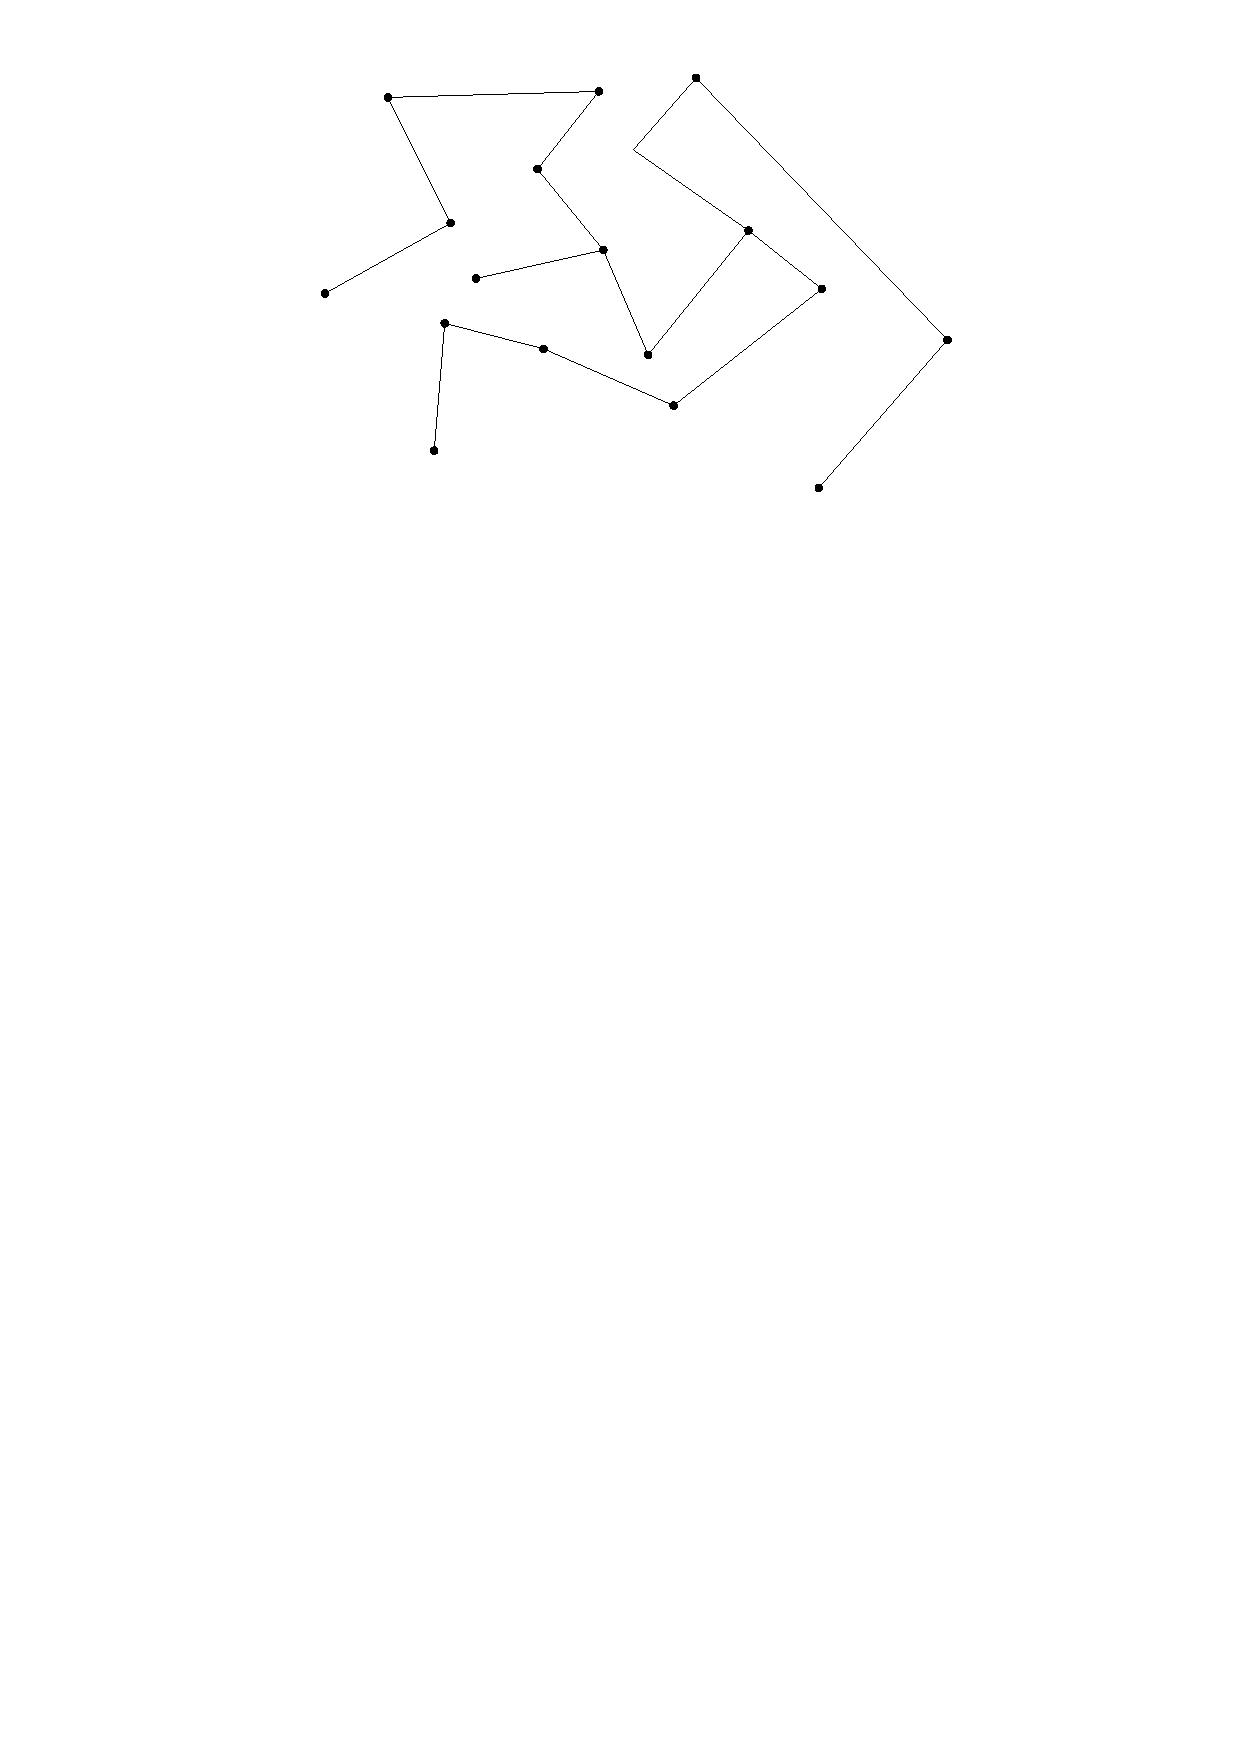
\includegraphics[scale=.5]{graphics/randomLinkage.pdf}
% % \end{center} 
% % \caption{A linkage with joints.}
% % \end{figure} 
% % \begin{figure}[h]
% % \begin{center}
% % 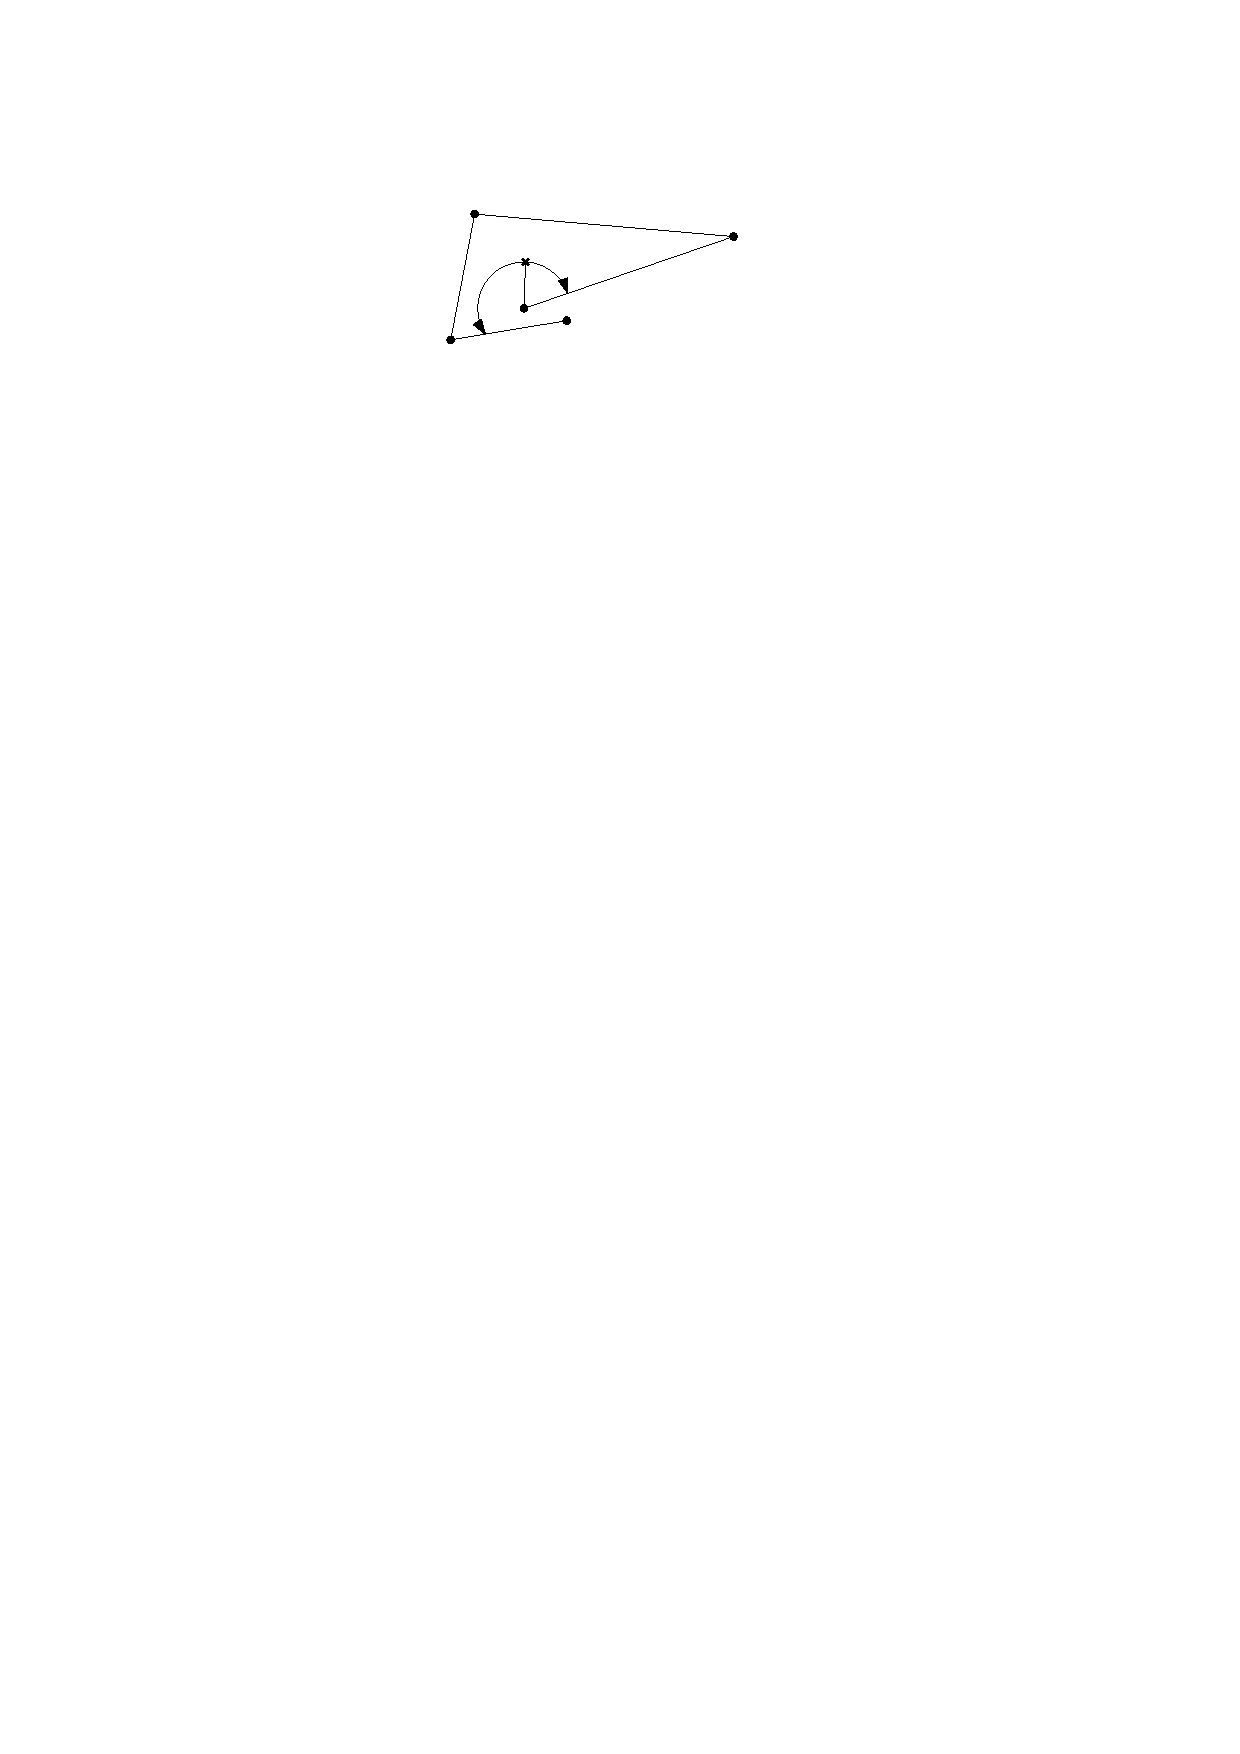
\includegraphics{graphics/freeJointPinnedJoint.pdf}
% % \end{center} 
% % \caption{The cross represents a free joint; the pinned joints are denoted as disks.  The range of 
% motion shown by the arc describes the continous configuration space of the linkage.}
% % \end{figure} 
% % 
% % For illustrations in the remainder of this paper, free joints will be represented as crosses and 
% pinned joints will be represented as disks.
%I) Algorithm Complexity
%	a) Algorithm
%		procedure of calculations
%		has a running time
%		utilizes resources
%		goal: have an algorithm that runs quickly and utilizes a small amount of resources
%	b) Qualitative Analysis of Algorithms
%		worst case running time
%		brute force
%		efficiency
%	c) Spaces of Algorithms
%		polynomial time
%		PSPACE
%		NP
%		P
%		NP-Complete
\section{Algorithm Complexity}
\textit{Algorithms} are a list of instructions executed with a given input.  
%When an algorithm executes its procedures, its efficiency can be measured in terms of units of resources such as memory and time. %it takes to complete the procedure of calculations.  
The efficiency of an algorithm can be measured in terms of the amount of resources it uses such as time, memory, and power.
Ideally, a desirable algorithm would primarily have a small run time and secondarily utilize a small amount of resources.

%ELABORATE ON RAM DESCRIPTION
The time and space used by an algorithm is measured with units defined by a model of computation.
The actual running time of an algorithm depend on a variety of factors for example: the processor, the hardware, the temperature, etc.
Mathematical models of computation have been developed to measure running time of algorithms independent of the machine it runs on.
One of the oldest and most popular models is the random access machine (RAM) model.
RAM measures the unit of space in the number of words used where each word can store an arbitrary integer.
In the real RAM, each word can store an arbitrary real number.
The units of time is measured in the number of arithmetic operations and number of memory accesses (read or write). 

% \subsection{Qualitative Analysis of Algorithms  }
%Determining the time and space that algorithms use determine their efficiency. 
The \textit{running time} of an algorithm on a given input, is the time it takes to terminate.% an algorithm with the input. 
The \textit{worst-case} running time is the largest running time over all inputs of a given size $N$.  
It is a function of $N$, it is usually monotonically increasing function since larger inputs tend to take more time to process.
The key parameter of the efficiency of an algorithm is the growth rate of its worst case running time in terms of $N$.
An algorithm is said to be \textit{efficient} if the time needed to perform the list of instructions can be determined from a polynomial. 
Devising an efficient algorithm for a given problem is often a difficult task.% however one can typically solve a problem by trying all possi
%if it achieves qualitatively better worst-case performance, at an analytical level, than brute force search.% \cite{kleinberg2006algorithm}.
% \subsection{Categorization of Algorithms}
%For combinatorial problems, as the number of inputs of the problem grows, the solution space tends to grow exponentially.  
% For decision problems, 
% n general, as problems grow, it is desirable to minimize 
% Formally, we quantify running time with Big O notation.

The growth rate of running times are typically compared upto constant vectors.
Let $f$ and $g$ be defined on some subset of $\bbR$.  
$f(x) = O\left(g(x)\right)$ if and only if there exists a constant $M$ and $x_0$ such that $$\left\vert g(x)\right\vert \leq M \left\vert f(x) \right\vert$$
for all $x \geq x_0$



% \subsubsection{P and NP}
% There are various types of running times; the running time that we will focus on in this thesis is 
% polynomial running time ($\P$), nondeterministic polynomial running time ($\NP$), and 
% non-deterministic polynomial complete running time ($\NP$ complete).

%An algorithm has a \textit{polynomial running time} if there is a polynomial function $p$ such that for every input string $s$, the algorithm terminantes on $s$ in at most $O\left( p \left( \left\vert s \right\vert\right)\right)$ steps.  

%To categorize problems \cite{kleinberg2006algorithm}, we ask the following:
\subsection{Complexity Classes}
Problems can be categorized by their running times.
Each algorithm computes a function $f(I)$ on an input $I$, however many different algorithms can compute the same function.
Algorithms are differentiated by their running times but the function is characterized by the fastest algorithm that can compute it.
A problem can be formulated as follows, given input $I$ find $f(I)$.

Problems can be categorized into complexity classes based on the fastest algorithms that solve them.
The class of problems that can be solved in polynomial running time is called the \textit{polynomial time} class, $\P$.

A second property of problems is whether its solution can be verified efficiently.  
This property is independent of whether it can be solved efficiently.  
$B$ is said to be an \textit{efficient certifier} for a problem $X$  if the following properties hold:
\begin{itemize}
\item[(i)] $B$ is a polynomial-time algorithm that takes two inputs $s$ and $t$.
\item[(ii)] There exists a polynomial function $p$ such that for every string $s$, we have $s \in X$ if and only if there exists a string $t$ such that $\vert t \vert \leq p\left( \vert s \vert \right)$ and $B(s,t) = \text{'yes'}$.
\end{itemize}

The class of problems which have an efficient certifier is said to be the \textit{nondeterministic polynomial time} class, $\NP$. 
We continue with the definitions for $\NP$-hard and $\NP$-complete.
A problem is $\NP$-hard if every problem in $\NP$ can be reduced to it in polynomial time.
A \textit{polynomial time reduction} is when arbitrary instances of problem $Y$ be solved using a polynomial number of standard computational steps, plus a polynomial number of calls to a black box that solves problem $X$, i.e. $Y$ is reduced in polynomial time to $X$.
A problem is $\NP$-complete if it $\NP$ and $\NP$-hard, i.e. $\NP$-complete = $\NP \cap \NP$-hard.


 %and what an efficient certification is.  
%This facilitates the reader for the definitions and illustrate complexity better. 
 
% \subsection{Reduction}



% \subsection{Independent Sets and Vertex Covers}
% To illustrate what a reduction is, we cover an example of independent sets and vertex covers.  
% Recall the definitions of an independent set and vertex cover.
% Given a graph $G = (V,E)$, a set of vertices $S \subset V$ is \textit{independent} if no two vertices in $S$ are joined by an edge. 
% A \textit{vertex cover} of a graph $G = (V,E)$  is a set of vertices $S \subset V$ if every edge $e \in E$, has at least one end corresponding in $S$.

% \begin{thm}\label{thm:ch1-complexity-1}
% Let $G = (V,E)$ be a graph.  
% Then $S$ is an independent set if and only if its complement $V-S$ is a vertex cover.
% \end{thm}
% \begin{proof}
% If $S$ is an independent set. Then for any pair of vertices in $S$, the pair are not joined by an edge if and only if for any $v_1, v_2 \in S$, $e = \left( v_1, v_2 \right) \not \in E$.  
% We have two cases.  
% The first case is if $v \in S$, then any vertex $u \in V$ that forms an edge $e = (v,u) \in E$ must reside in $V-S$. 
% The second case is if there is an edge which no pair of vertices is in $S$, then both vertices are in $V-S$.  
% Both cases together imply that every edge has at least one end corresponding in $V-S$. 

% If $V-S$ is a vertex cover.  
% Every edge $e \in E$ has at least one vertex in $V-S$.  
% The two possible cases, the first case is that the second vertex is in $V-S$, and the second case is that the second vertex is in $S$.  The first case would yield $S = \emptyset$.  
% The second case implies that the edge $e \in E$ has exactly one vertex in $V-S$ and exactly one vertex in $S$.  
% $V-S$ is a vertex cover would disallow $S$ to have a pair of vertices to form an edge in the graph.
% \end{proof}
% Theorem \ref{thm:ch1-complexity-1} allows for problem reductions for independent set and vertex cover problems.

% % \subsubsection{Reduction of the Independent Set and Vertex Cover Problem}
% There are two problems for the independent set: an optimization problem and a decision problem.
% \begin{prob}[Optimization of an Independent Set in $G$]\label{prob:maxindependentset}
% Given a graph $G$, what is the largest independent set in $G$?
% \end{prob}
% \begin{prob}[Decision of an Independent Set of Size $k$]\label{prob:kindependentset}
% Given a graph $G$ and a number $k$, does $G$ contain an independent set of size at least $k$?
% \end{prob}
% % [NEEDS TO PROVE REDUCIBILITY IN THIS PARAGRAPH BELOW]
% % An algorithm that solves the optimization problem automatically solves the decision problem of the 
% % independent set.  An algorithm that solves the decision problem for all size $k$ solves the 
% % optimization problem where the decision is "yes" for the largest value of $k$.  This establishes a 
% % reduction of the optimization problem to the decision problem and vice versa. 
% % [NEEDS TO PROVE REDUCIBILITY IN THIS PARAGRAPH ABOVE]
% Consider an algorithm $A$ that determines whether $G$ contains an independent set of size $k$.  
% By querying $A$ with $k=1,2,...,\vert V \vert$, one can find a maximal independent set size in $G$.
% Conversely, if we have an algorithm $B$ that can the largest independent set in $S \subset V$, then we know the order of $S$, $\vert S\vert$.  
% Any subset of $S$ is also an independent set; any subset $W \subset V$ such that $\vert S \vert < \vert W \vert \leq \vert V \vert$ is not independent.  
% While $B$ is an algorithm that solves Problem \ref{prob:maxindependentset}, $B$ can be leveraged to solve Problem \ref{prob:kindependentset}.  
% Likewise, $A$ solve Problem \ref{prob:kindependentset} but can be leveraged to solve Problem \ref{prob:maxindependentset}.


%FROM COMPLEXITY, USE THE PAPER TO SHOW THAT OUR DECISION PROBLEMS ARE HARD.


% Other classes of problems are $\NP-\text{complete}$ and 
% $\NP-\text{hard}$.  $\NP-\text{complete}$ is a class of decision problems.  A problem $\mathcal{C}$ 
% is said to be $\NP-\text{complete}$ if $\mathcal{C} \in \NP$ and every problem $\mathcal{D} \in 
% \NP$ 
% is reducible to $\mathcal{C}$ in polynomial time.  $\NP-\text{hard}$ is a class of problems that 
% are 
% at least as hard as $\NP-\text{complete}$ problems.
\subsection{RSA Cryptosystem}
Cryptography is the study of secure communication between parties in an untrusted or unsecure communication channel.
Cryptography has three primary purposes for secure communications: provide confidentiality, authenticate entities, and verification of data.
Modern cryptography is based on hard math problems such as integer factorization, discrete logarithmic problem, and pre-image problems. 
Hard math problems are not found in $\P$ and found in $\NP$.
In most forms of modern cryptography, \textit{keys}, are data parameters used to form function outputs for the use in a communication channel.
There are three common types of keys in cryptography:
\begin{enumerate}
\item A \textit{secret key} is known by certain entities.  Typically a secret key is used by entities to encrypt and decrypt data that is communicated over an untrusted channel.  Secret keys require a secure channel to exchange between all entities.
\item When there are no means to exchange secret keys, one can use a private and public key scheme.
A \textit{public key} is a key that can be shared with any entity, i.e. trusted and untrusted entities can know it.
The \textit{private key} is a key that is kept to one entity. It is treated like a secret key and should only be known to that entity.
\end{enumerate}
A \textit{cryptosystem} is a suite of algorithms used to establish secure communication channel between parties. 
The RSA cryptosystem is the first practical cryptosystem in modern cryptography that allows for encryption of data (confidentiality), authentication of entites, and verify message integrity using just one underlying hard math problem, integer factorization.

RSA is named after its second inventors, Ron Rivest, Adi Shamir, and Leonard Adelmen.
These three individuals devised and published the algorithm in 1977.
The original inventor of RSA was Clifford Cocks in 1973 however, it was only known to the public since 1997 that Clifford Cocks was the original inventor because his was was classified by Government Communication Headquaters, an intelligence agency of the United Kingdom.

For the RSA cryptosystem, we first want to pose the communication security problem.  
Suppose we have two entities, Alice and Bob, that wish to communicate over an unsecure channel.
Should Alice and Bob agree to using RSA, each entity will have a pair of keys, a private key and a public key.
Most implementations of RSA use the following key derivation \cite{rivest1978method}:
\begin{enumerate}
\item Let $n=p\cdot q$ where $p$ and $q$ are randomly chosen prime numbers.
\item Choose an integer $e$ such that $1 < e \leq \phi (n)$ and $gcd\lr{e,\phi\lr{n}}=1$ where $\phi$ is the Euler totient function.
\item Let $d \equiv e^{-1} \mod \phi(n)$.
\end{enumerate}
The RSA cryptosystem is based around the following formula:
$$\left(m^e\right)^d \mod n= \left(m^d\right)^e \mod n\equiv m \mod n$$
where we have natural numbers $e$, $d$, $m$, and $n$, such that $m < n$ and $gcd(m,n)=1$.


%explain fermat's little theorem here
If Alice derives a public and private key in the manner described, her public key is $(n,e)$ and her private key is $d$.
Suppose Bob wants to send Alice a message $M$.  
Bob will represent $M$ in binary form, $m$.
%Suppose Bob wants to send Alice a natural number $m$ to Bob over an untrusted or insecure communication channel.  
%$m$ may represent a binary code of a message.
Alice sends her public key $(n,e)$ to Bob and keeps her private key $d$ secret.  
If $gcd(m,n)\neq 1$, then Bob modifies $m$ by padding $m$ with additional digits so that $m$ becomes co-prime with $n$.
There are efficient padding schemes to modify $m$ such that $m$ and $n$ are co-prime \cite{jonsson2003public}.
Bob sends the following value, $c$, to Alice:
$$c \equiv m^e \mod n$$
$c$ is said to be a ciphertext.
Alice can decrypt the ciphertext and recover $m$ by computing:
$$ m \equiv c^d \mod n = \lr{m^e}^d \mod n$$

The RSA cryptosystem is based on integer factorization and the RSA problem, given $n$ where $n=p\cdot q$ where $p$ and $q$ are prime numbers, find $p$ and $q$.
For sufficiently large integers, factorization and the RSA problem becomes very difficult.  
If there were an algorithm that solved integer factorization in polynomial time, then one can also solve the RSA problem as well.
Suppose a third party listens into the conversation and knows Alice's public key $(n,e)$ and the ciphertext $c$.
If the the third party can factor $n = p\cdot q$ then the attacker can computer $\phi(n)$ and compute $d \equiv e^{-1} \mod \phi(n)$ using the extended euclidian algorithm.
Once they have $d$, the attacker can compute $m \equiv c^d \mod n$.

Currently, the most efficient factorization algorithm is the general number sieve algorithm \cite{lenstra1993number}.
It's an exponential running time algorithm.
If a polynomial running time algorithm for integer factorization existed, it would allow for compromise of security that is provided to communicating parties by the RSA cryptosystem.
It would allow for a reduction of the integer factorization problem, a problem that exists in $\NP$ but not $\P$.
The algorithm would allow for an adversary to attack RSA \cite{menezes1996handbook} in polynomial time.



\section{Satisfiability}
Let $x_1, \dots, x_n$ be boolean variables.  A boolean formula is a combination of conjunction, 
disjunctions, and negations of the boolean variables $x_1,  \dots, x_n$.   
A \textit{clause} is a disjunction of distinct literals.  
A \textit{literal} is a variable or a negated variable, $x_i$ or $\bar{x}_i$, for $i = 1,\dots,n$. 
A boolean formula is \textit{satisfiable} if one can assign true or false value to each variable so that the formula is true. 
It is known that every boolean formula can be rewritten in \textit{conjunctive normal form} (CNF), a conjunction of clauses, via DeMorgan's law and distributive law.   
Furthermore, it is also known that every boolean formula can be written in CNF such that each clause has exactly three literals. 
This form is called 3-CNF.  
For example, consider the clause $A \lor B \lor C \lor D \lor E$. 
This clause can be rewritten in 3-CNF form as $(A \lor B \lor x_1) \land (\lnot x_1 \lor C \lor x_2) \land (\lnot x_2 \lor D \lor E)$ where $x_1$ and $x_2$ are literals that allow us to form 3-CNF clauses.
Here are the problem statements for satisfiability:
%\textit{3-SAT problem}.
\begin{prob}[Satisfiability Problem (SAT)]\label{prob:Satisfiability-1}%Problem/Question
Given a boolean formula, is it satisfiable? \cite{skiena2009algorithm}
\end{prob} 
\textit{Brute force} is when an algorithm tries all possibilities to see if any formulates a satisfiable solution.
It is clear that SAT is decidable in exponential time by testing all possibilities.
This is callled a brute force solution.
It is not known whether SAT admits a polynomial time solution, that is whether it is in $\P$. 
\begin{prob}[3-SAT Problem]
Given a boolean formula in 3-CNF, is it satisfiable?
\end{prob}
The problems we focus on in this thesis have a geometry.  
A special geometric 3-SAT problem is that Planar 3-SAT Problem.   
Given a 3-CNF boolean formula, $\Phi$, with $n$ variables and $m$ clauses.
  We define the \textit{associated graph} $A(\Phi)$ as follows: the vertices correspond to the variables and clauses in $\Phi$.  
  We place an edge in the graph if variable $x_i$ appears in clause $C_j$.

  \begin{figure}[htbp]
	\centering
	\includegraphics[width=0.7\columnwidth]{graphics/fig-assoc-hex}
	\caption{Left: the associated graph $A(\Phi)$ for a Boolean formula $\Phi$.
Right: the schematic layout of the variable, clause, and transmitter gadgets in the auxiliary construction showing in Section \ref{sec:auxiliaryConstruction}}
	\label{fig:assoc}
\end{figure} 
\begin{prob}[Planar 3-SAT]
 Given a boolean formula $\Phi$ in 3-CNF such that its associated graph is planar, decide whether it 
is satisfiable is a \textit{3-SAT problem}.
\end{prob}
Figure \ref{fig:assoc} is associated to a family of boolean formulas.  
One such associated boolean formula is:
$$(x_1 \lor x_3 \lor \lnot x_5) \land (\lnot x_1 \lor \lnot x_2 \lor x_3) \land (\lnot x_3 \lor x_4 \lor \lnot x_5) \land (x_2 \lor x_4 \lor \lnot x_5) \land ( \lnot x_1 \lor x_2 \lor x_5)$$
Note that the figure establishes an edge relation between variables and clauses whereas the clauses in boolean formulas do not have variables but literals of variables.
\begin{prob}[Not All Equal 3 SAT Problem (NAE3SAT)]\label{prob:Satisfiability-2}%Problem/Question
Given a boolean formula in 3-CNF, is it satisfiable so that each clause contains a 
true and a false literal?
\end{prob}

Problems \ref{prob:Satisfiability-1}---\ref{prob:Satisfiability-2} are known to be NP-hard and are often used to show other problems are NP-hard as well \cite{lichtenstein1982planar,karp1972reducibility}.
%draw a picture for this one.


% 
% Given a boolean 3-SAT formula $B$, define the associated graph of $B$ as follows:  
% \begin{equation}\label{eqn:sat-1}
% G(B) = \left(\set{v_x}{v_x\text{ represents a variable in }B} \cup \set{v_C}{v_C\text{ represent a 
% clause in }B}  , \set{\left( v_x, v_C\right) }{x \in C \text{ or } \bar{x} \in C}  \right) 
% \end{equation} 
% If $G(B)$ in equation (\ref{eqn:sat-1}) is planar, then $B$ is said to be a \textit{Planar 3-SAT 





%3-SAT, PLANAR 3-SAT, NAE3SAT are NP hard [ADD REFERENCE].  THE PROOF FOR THESE REDUCTIONS ARE NOT 
%OBVIOUS BUT ARE SHOWN [HERE, THERE, AND OVER THERE] respectively.
% Definition 1. (PLANAR 3-SAT) Let Φ be a
% Boolean formula in 3-CNF. The formula graph of
% Φ, G(Φ), has one variable-vertex vx for each variable
% x and one clause-vertex vC for each clause C. The
% variable-vertices vx are connected by edges to form a
% variable cycle, and for each clause-vertex vC an edge
% (vC, vx) is added if C contains either literal x or x.
% We say Φ is planar iff G(Φ) is planar. The PLANAR
% 3-SAT problem is equivalent to the 3-SAT problem
% restricted to planar formulae.
% Theorem 2.1. (Lichtenstein [14] Theorem 2)
% PLANAR 3-SAT is NP-complete
% \begin{prob}[Planar 3 SAT Problem]
%  A planar 3SAT instance is a 3SAT instance for which the graph built using the following rules is 
% planar:
% \begin{enumerate}
%  \item add a vertex for every $x_i$ and $\bar{x}_i$
%  \item add a vertex for every clause $C_j$
%  \item add an edge for every $\left(x_i,\bar{x}_i \right)$ pair
%  \item add an edge from vertex $x_i$ (or $\bar{x}_i$) to each vertex that represent a clause that 
% contains it
%  \item add edges between two consecutive variables $(x_1,x_2)$, $(x_2,x_3)$, $\dots$,$(x_n,x_1)$
% \end{enumerate}
% In particular, rule 5 builds a "backbone" that splits the clauses in two distinct regions.
% \end{prob}

%%Universality component
%\subsection{Logic Engine}
%The logic engine simulates the well known Not All Equal 3 SAT Problem (NAE3SAT).  
%%add figure of logic engine.
%\subsection{Construction of the Logic Engine}
%The components of the logic engine are as follows: the rigid frame, the shaft, the armatures, 
%the chains, and the flags.  The \textit{rigid frame} is a rectangular enclosure with a horizontal 
%shaft place at mid-height.  The \textit{armatures} are concentric rectangular frames contained 
%within the rigid frame.  Each armature can rotate about the shaft; other motions on the armature 
%are disallowed.  Given an NAE3SAT, for each variable there is a corresponding armature. On each 
%armature, there are chains.  A pair of \textit{chains}, $a_j$ and $\bar{a}_j$ correspond to the 
%variable $x_j$ and $\bar{x}_j$ respectively.  The pair is placed on each armature, reflected at a 
%height of $h$ above and below the shaft, i.e. one place above the shave at a height of $h$, the 
%other placed below the shaft at a height of $-h$.
%%insert an armature graphic
%
%\subsection{Encoding the Logic Engine}
%For each clause of an NAE3SAT, there exists a set of corresponding chains, namely the $h^\text{th}$ 
%clause is the set of chains on the armatures at the $h^\text{th}$ row above and below the shaft. A 
%chain is \textit{flagged} if the corresponding variable resides within the clause.  The flag can 
%point in either the left or right directions indicating a truth assignment for that variable within 
%the clause.  A flag is attached to the $i^\text{th}$ chain of every $a_j^\text{th}$ and 
%$\bar{a}_j^\text{th}$ chain with the following exceptions:
%\begin{enumerate}
% \item if the variable $x_j$  is in clause $C_i$, then link $i$ of $a_j$ is unflagged,
% \item if the variable $\bar{x}_j$ is in clause $C_i$, then link $i$ of $a_j$ is unflagged.
%\end{enumerate}
%\begin{thm}\label{thm:Satisfiability-1}
% An instance of $NAE3SAT$ is a ``yes'' instance if and only if the corresponding logic engine has a 
%flat, collision-free configuration.
%\end{thm}
%\begin{pf}
% If an instance of $NAE3SAT$ is a ``yes'', then every clause in $C$ contains at least one true 
%variable and one false variable.  Now suppose the following truth assignment:
%\begin{equation}\label{eqn:Satisfiability-1}
% t\left( x_j \right) = \left\lbrace\begin{array}{cr}
%  1 & x_j\text{ and }\bar{x}_j \text{are placed at the top and bottom respectively}\\
%  0 & x_j\text{ and }\bar{x}_j \text{are placed at the bottom and top respectively}\\
% \end{array}\right.
%\end{equation}
%For each clause $c_i \in C$, there exists a variables in $c_i$ such that $t\left( y_i \right) = 1$ 
%and $t\left( z_i \right) = 0$.  This implies that there exists an unflagged chain in the 
%$i^\text{th}$ and $-i^\text{th}$ row of the frame.  To avoid a collision in each row, trigger the 
%flags to point towards the unflagged link. Thus, the corresponding logic engine has a 
%flat, collision-free configuration.
%
%If the corresponding logic engine has a flat, collision-free configuration, then there must exist 
%an unflagged link in each row.  Without loss of generality, we have that the variables $y_j$ and 
%$z_i$ is in clause $C_i$ such that $t\left( y_i \right) = 1$ and $t\left( z_i \right) = 0$ for each 
%$i$.  Thus, we have an instance of $NAE3SAT$ is a ``yes'' instance. \cite{BET+99}
%\end{pf}

\section{Contribution}
The \emph{realizability} problem for a polygonal linkage asks whether a given polygonal linkage has 
a realization (resp., orientated realization). For a weighted planar (resp., plane) graph,, it asks 
whether the graph is
the contact graph (resp., ordered contact graph) of some disk arrangement with specified radii. 
These problems, in general, are known to be NP-hard. Specifically, it is NP-hard to decide whether a 
given planar (or plane) graph can be embedded in $\RR^2$ with given edge lengths~\cite{CDD+10,EW90}. 
Since an edge of given length can be modeled by a suitably long and skinny rhombus, the 
realizability of polygonal linkages is also NP-hard. The recognition of the contact graphs of unit 
disks in the plane (a.k.a. coin graphs) is NP-hard~\cite{BK98}, and so the realizability of weighted 
graphs as contact graphs of disks is also NP-hard. However, previous reductions crucially rely on 
configurations with high genus: the planar graphs in~\cite{CDD+10,EW90} and the coin graphs 
in~\cite{BK98} have many cycles.

In this thesis, we consider the above four realizability problems when the union of the polygons 
(resp., disks) in the desired configuration is simply connected (i.e., contractible). That is, the 
contact graph of the disks is a tree, or the ``hinge graph'' of the polygonal linkage is a tree (the 
vertices in the \emph{hinge graph} are the polygons in $\PP$, and edges represent a hinge between 
two polygons). Our main result is that realizability remains NP-hard when restricted to simply 
connected structures.
 
 % \subsection{Problem Statement} 
%write up thm 1, 2 (unoriented versions of the problem)
%write up thm 3, 4 (oriented versions of the problem)
\begin{thm}\label{thm:hinge2}
It is strongly NP-hard to decide whether a polygonal linkage whose hinge graph is a \textbf{tree} can be realized.
\end{thm}
\begin{thm}\label{thm:hinge3}
It is strongly NP-hard to decide whether a polygonal linkage whose hinge graph is a \textbf{tree} can be realized with fixed orientation.
\end{thm}
Our proof for Theorem \ref{thm:hinge3} is a reduction from {\sc Planar-3-SAT} (P3SAT): decide whether a given Boolean formula in 3-CNF with a planar associated graph is satisfiable. 
Our proof for Theorem \ref{thm:hinge2} is a reduction from {\sc Not-All-Equal-3-SAT} (NAE3SAT): decide whether a given Boolean formula in 3-CNF  is it satisfiable so that each clause contains a true and a false literal?


\begin{thm}\label{thm:hinge}
It is NP-Hard to decide whether a polygonal linkage whose hinge graph is a tree can be realized 
(both with and without orientation).
\end{thm}

\begin{thm}\label{thm:disk}
It is NP-Hard to decide whether a given tree (resp., plane tree) with positive vertex weights
is the contact graph (resp., contact graph) of a disk arrangements with specified radii.
\end{thm}

The unoriented versions, where the underlying graph (hinge graph or contact graph) is a tree can 
easily be handled with the logic engine method (Section~\ref{sec:logic}). We prove 
Theorem~\ref{thm:hinge} for \emph{oriented} realizations with a reduction from {\sc Planar-3SAT} 
(Section~\ref{sec:hinge}), and then reduce the realizability of ordered contact trees to the 
oriented realization of polygonal linkages by simulating polygons with arrangements of disks 
(Section~\ref{sec:disk}).


% \subsection{Decidability of Problem} test
% \subsection{Hexagonal Locked Configuration}\section{Related Work and Results}
Boris Klemz's Master's thesis ``Weighted Disk Contact Graph'' shows the Unit Disk Touching Graph Recognition problem is NP-Hard.  
% In Chapter 2 we investigate recognition problems with uniform (and ρ-bounded) radii. In Section 2.1 we consider the Unit Disk Touching Graph Recognition (UDT) problem and strengthen the result of Breu and Kirkpatrick [BK98] by showing that the UDT problem is NP-hard even for outerplanar graphs. On the positive side, we provide a linear-time algorithm for deciding the UDT problem in caterpillars. In this section we also briefly consider ρ-bounded Disk Touching Graph Recognition and show that for spiders this problem can be solved in linear time in the Real RAM model. In Section 2.2 we extend our result from the previous section by showing that the Unit Disk Touching Graph Recognition with fixed Embedding (UDTE) problem is also NP-hard, even for outerplanar graphs.
% In Chapter 3 we explore the more general scenario with fixed but not necessarily uniform radii. In Section 3.1 we consider the Disk Touching Graph Recognition with fixed Radii (DTR) problem and strengthen the result by Breu and Kirkpatrick [BK98] by showing that the DTR problem is NP-hard even for stars. We also show that for any cycle and a corresponding radius assignment there exists a realizing disk touching graph. In contrast, in Section 3.2 we devise a linear-time algorithm for deciding the Disk Touching Graph Recognition with fixed Radii and Embedding (DTRE) problem for stars in the Real RAM model.
% In Chapter 4 we concern ourself with the scenario in which a seed assignment is required to be respected. In Section 4.1 we strengthen the result of Atienza et al. [AdCC+12] by showing that the Disk Touching Graph Recognition with fixed Seeds (DTS) prob- lem is NP-hard even for trees. In Section 4.2 we combine this scenario with assigning fixed radii, more specifically uniform radii. We show that the Unit Disk Touching Graph Recognition with fixed Seeds (UDTS) problem is NP-hard, even for paths, implying that the Unit Disk Touching Graph Recognition with fixed Seeds and Embedding (UDTSE) problem is also NP-hard even for paths.
It also improves the Breu and Kirkpatrick result on Disk Touching Graph Recognition problem \cite{klemzthesis,BK98}.\chapter{Decision Problems for Hinged Polygons and Disks}\label{chapter:logicEngine}
\section{The Logic Engine}
%explain what is the connection between the title of the chapter and the technical details of the chapter.  
%expand a bit about the gadget and how it is a decision problem for Hinged Polygons and Disks.
The \textit{logic engine} is a planar, mechanical device that simulates an instance NAE3SAT problem. It was introduced in Bhatt et. al. \cite{BC87}.
\subsection{Construction of the Logic Engine}

\begin{figure}[!h]
\begin{center}
\includegraphics{graphics/LogicEngineFrameFigure1Scaled.pdf}
\caption{A logic engine frame with veritical armatures and a horizontal shaft.}
\label{fig:LogicEngineFrameFigure1.pdf}
\end{center}
\end{figure}

For a given a boolean formula, $\Phi$, in 3-CNF with $n$ variables and $m$ clauses, we construct a logic engine. The logic engine has a \textit{rigid frame} which houses the mechanical components of the the logic engine.  The rigid frame is the boundary of which the logic engine can operate within.  The \textit{shaft} is a horizontal line segment that is placed at mid-height of the rigid frame. 
The \textit{armatures} are veritical line segments whose midpoints are on the shaft.  
Each armature has two orientations with respect to the shaft. 
There will be some flags on each armature that will be described later.
The armatures each have length $2n$ units, the shaft has length $m$ units, and the frame has a height of $2n$ and width of $m$ units.


\begin{figure}[!h]
\begin{center}
\includegraphics{graphics/LogicEngineFrameFigure1halfScaled.pdf}
\caption{A logic engine that corresponds to a boolean formula in NAE3SAT form, $\Phi$.  The picture shows the outer rigid frame, the shaft, the armatures that correspond to the variables in $\Phi$, with oriented flags.}\label{fig:LogicEngineFrameFigure1halfScaled.pdf}
\end{center}
\end{figure}

  Each armature corresponds to a variable in $\Phi$. There are two literals for each variable, i.e. the literal $x_j$ and the negated literal 
 $\bar{x}_j$.   
 %Flagging arragement indicates the relationship of the boolean literal's existence within a clause.   
 To describe the flagging arrangement, first partition each armature into $2m$ units, vertical line segments. Label the segments on the $j^\text{th}$ armature starting from the shaft by $\ell_{j,1},\ldots,\ell_{j,n}$ on one side and  $\bar{\ell}_{j,1},\ldots,\bar{\ell}_{j,n}$ on the other side of the shaft.  
 Attach regular triangles, called \textit{flags}, to some of these segments. 
 Each segment is either flagged one or zero flags, i.e. \textit{flagged} or \textit{unflagged}. If the literal $x_j$ is found in clause $C_k$, then $\ell_{j,k}$ is unflagged.
   If the literal $\bar{x}_j$ is found in clause $C_k$, then $\bar{l}_{j,k}$ is unflagged.

Each flag has two orientations with respect to armature it is attached to.  Each flag has four potential positions, the flag can reflect left or right about the armature and the armature can reflect up or down about the shaft.
\begin{figure}[!h]
\begin{center}
\includegraphics{graphics/LogicEngineFrameFigure2Scaled.pdf}
\caption{A logic engine constructed from the boolean formula $\Phi = C_1 \cap C_2 \cap C_3$.}
\label{fig:LogicEngineFrameFigure2Scaled.pdf}
\end{center}
\end{figure}
The \textit{flags} are equilateral triangles
attached to the armatures.  The placement of the flags is dependent on the instance of the NAE3SAT 
boolean formula. Each flag as two orientations. 

For the NP hardness reduction in Theorem \ref{thm:LogicEngineV3-2} we need to make sure that all parameters in the logic engine can be specified polynomially in terms of the size of the boolean formula. Given $\Phi$, the corresponding logic engine is constructed as follows: all components will be specified with a 
quantity and coordinates defined as polynomials in $m$ and $n$.

\begin{center}
	\begin{table}[H]\label{LogicEngineV3PolynomialTable}
		\begin{tabular}{|c|c|c|}
			\hline
			Component & Quantity &  Set Definition\\ \hline
			Rigid Frame&1&$\set{(x,y)\in\bbr^2}{ \text{The boundary of }\left[ \frac{1}{2} , n + \frac{1}{2}\right] \times \left[ -m, m \right]}$\\ \hline
			Shaft&1&$\set{(x,y) \in \bbr^2}{x \in \left[\frac{1}{2}, n + \frac{1}{2}\right] \text{ and } y=0 }$\\ \hline
			Armatures & n & For the $j^\text{th}$ armature we have $\set{(x,y)\in\bbr^2}{x = j \text{ and } y \in [-m,m] }$\\ \hline
			Flags&$2mn-3m$& if $\ell_{j,k}$ is flagged then the attached flag is a regular triangle with side length 1.\\ \hline
		\end{tabular}
	\caption{The quantity and coordinates of the logic engine components.}
	\end{table}
\end{center}

\subsection{The mechanics of the logic engine}
In any of the following cases, a \textit{collision} of flags occurs:
\begin{enumerate}
\item flags in the same row on adjacent armatures point toward each other.
\item a flag from the rightmost armature $A_n$ points towards the outer rigid frame.
\item a flag from the leftmost armature $A_1$ points inwards of $A_1$.
\end{enumerate}

\begin{figure}[!htbp]
\begin{center}
\includegraphics[scale=.5]{graphics/logicEngineCollisions.pdf}
\caption{(a) Illustrates a adjacent flag collision at the same height, (b) and (c) illustrates a 
rigid frame collision.}\label{fig:logicEngineCollisions.pdf}
\end{center}
\end{figure}
The logic engine representation corresponding to $\Phi$ is to be configured such that no 
horizontally adjacent flags collide and flags do not collide with the rigid frame. 
\begin{figure}[!htbp]
\begin{center}
\includegraphics{graphics/logicEngineValidConfigurations.pdf}
\caption{The following configuration of adjacent flags 
and flags that are adjacent to the rigid frame.}\label{fig:logicEngineValidConfigurations.pdf}
\end{center}
\end{figure}

\begin{lem}\label{lem:logicEngine1}A row has a collision-free configuration if and only if it has 
at least one unglagged armature. \end{lem}
\begin{proof}
% Suppose that the flag on armature $A_1$ is flagged.  If the flag is oriented left, then there 
% is a flag-frame collision.  If the flag is oriented to the right and if $A_2$ is flagged, then 
% $A_2$ must also be oriented to the right; otherwise will result in a flag-flag collision.  Now 
% suppose the $i^\text{th}$ armature's flag is oriented to the right.  $A_{i+1}$ is also oriented to 
% the right; otherwise will result in a flag-flag collision. By induction all flags will orient to 8187173855 135 500
% the right up to $n$.  Thus the $n^\text{th}$ flag will will collide with the rigid frame.

Suppose all armatures are flagged in a row.  The flag on armature $A_1$ must point to the 
right otherwise we result in a rigid frame collision.  $A_2$ must point to the right otherwise 
we result in a rigid frame collision.  Without loss of generality, $A_i$ and $A_{i+1}$ must 
point to the right in order to prevent an adjacent flag collision.  This implies that $A_n$ 
must also point to the right which results into a rigid frame collision.

A same argument holds with the argument beginning with the flag 
on the armature $A_n$ pointing to the left.  Thus there is no collision-free configuration with 
all armatures flagged.


Suppose there is an unflagged armature in a row.  Turn all flags towards the nearest unflagged 
armature.  If there are flags on $A_1$ and $A_n$, point toward the interior thus they do not 
collide with the rigid frame.  If there are flags on two consecutive armatures, they do not collide 
because the nearest unflagged armature cannot be between them.  Therefore the row has a 
collision-free configuration.
\end{proof}

A logic engine is said to be \textit{collision-free configurable} when every row has a collision-free configuration.
\begin{figure}[!ht]
\begin{center}
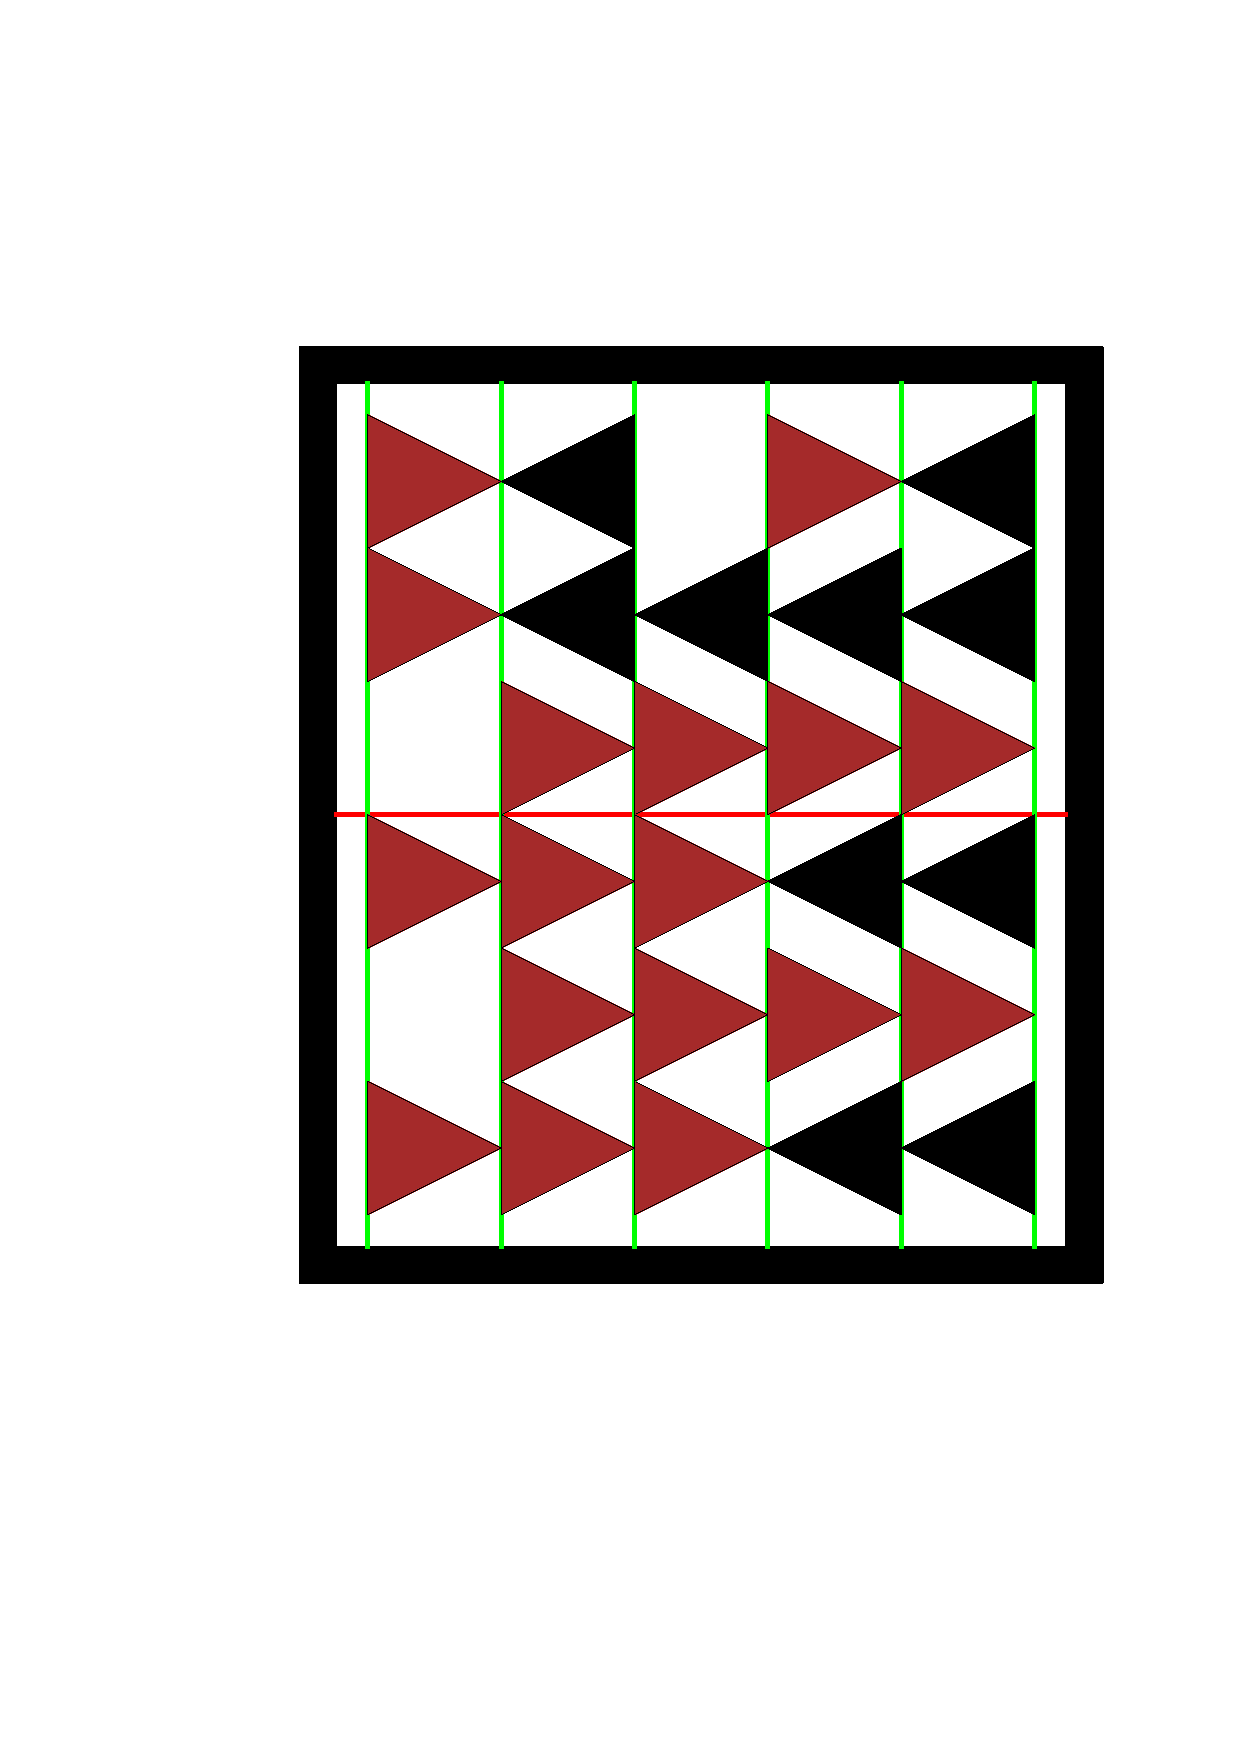
\includegraphics{graphics/LogicEngineFrameFigure5Scaled.pdf}
\caption{The logic engine from figure \ref{fig:LogicEngineFrameFigure2.pdf} whose armatures are rotated}\label{fig:LogicEngineFrameFigure5.pdf}
\end{center}
\end{figure}

\subsubsection{The Relationship of the Logic Engine and NAE3SAT}

We show that given an boolean formula in 3-CNF form, $\Phi$, and a truth assignement, $\tau$, where the variables are given a truth assignment such that there is at least one true literal and one false literal in each clause of $\Phi$, then the corresponding logic engine to $\Phi$ is collision-free configurable.
\begin{thm}\label{thm:LogicEngineV3-1}
 Given an instance of a $NAE3SAT$,  it is a ``yes'' instance if and only if the corresponding logic 
engine is collision-free configurable.
\end{thm}
\begin{proof}
Suppose we have an instance of a $NAE3SAT$ that is a ``yes'' instance. This implies that there is a 
truth assignment such that each clause contains a true and a false literal. Now consider the logic 
engine corresponding to this instance. We now 
show that it has a collision free configuration.

For variables that are true, configure the armatures such that the flags corresponding to the 
non-negated literals reside above the 
shaft and the flags that correspond to the negated literals reside below this shaft.  For variables 
that are false, configure the 
armatures in the opposite orientation.  Each clause corresponds to a pair of rows in 
the logic engine, one row for non-negated literals and one for negated literals.  Because the 
$NAE3SAT$ is a yes instance, every row contains at least one unflagged armature.  
By Lemma \ref{lem:logicEngine1}, every row  has a collision-free configuration.

Suppose we have an instance of a $NAE3SAT$ such that the corresponding logic engine has a 
collision-free configuration. By Lemma \ref{lem:logicEngine1} every row at least one unflagged 
armature.  The $k^{th}$ clause is represented by the $k^{th}$ rows above and below the shaft. If the 
literal $x_j$ is found in clause $C_k$, then the armature is unflagged in that row. If the literal 
$\bar{x}_j$ is found in clause $C_k$, then $\bar{l}_{j,k}$ is unflagged.  All flags 
corresponding to negated literals reside below the shaft and flags corresponding to non-negated 
literals reside above the shaft.  All together we have that every clause has a true literal and a 
false literal.  Thus, we have a 'yes' instance of the $NAE3SAT$.
\end{proof}
\begin{thm}\label{thm:LogicEngineV3-2}
Deciding whether a logic engine is collision-free configurable is NP-Hard.
\end{thm}
\begin{proof}
In table \ref{LogicEngineV3PolynomialTable}, we defined the components of the logic engine in terms of polynomials in $m$ and $n$. 
If there were a polynomial time algorithm that decides whether a given logic engine is collision-free configurable, then by Theorem \ref{thm:LogicEngineV3-1} we would have a polynomial time algorithm to decide whether an instance of the NAE3SAT is a 'yes' instance.  
Since NAE3SAT is NP-Hard \cite{NAE3SATisNPhard}, there is no such algorithm unless $P = NP$.
\end{proof}\section{Logic Engines Represented as Polygonal Linkages}   
In the previous section, we introduced the logic engine.  
This section builds an analogous structure that is formed from a polygonal linkage and we may interchangeably say subcomponent for polygon.
We can modify the mechanical structure of the logic engine to form a polygonal linkage.  
For a given a boolean formula, $\Phi$, in 3-CNF with $n$ variables and $m$ clauses,
the rigid frame is broken into two polygons, each polygon on the extremity of the structure.
The shaft is broken into $n$ polygons.
Each armature is broken into two parts, each part containing $m$ subcomponents.
In figure \ref{fig:HingedLogicEngineSmall.pdf}, each flag becomes a rectangle.

\begin{figure}[!htbp]
\begin{center}
\includegraphics{graphics/HingedLogicEngineSmall.pdf}
\caption{A logic engine realized as a polygonal linkage.}\label{fig:HingedLogicEngineSmall.pdf}
\end{center}
\end{figure}
\subsection{Construction of the Polygonal Linkage Logic Engine}
Suppose we are given an boolean formula with $m$ clauses and $n$ variables in 3-CNF form, $\Phi$, we construct the polygonal linkage similarly to the logic engine.
The corresponding polygonal linkage $P_\ell = (\PP,\HH)$ is detailed in Table \ref{tbl:hingedPolygonsv3-1a}.

% \begin{minipage}{\linewidth}
% \begin{center}
% \begin{table}\label{TBL:HingedPolygonsV3-1}
% 		$$\begin{array}{|l|c|c|c|}%TRY TO ADD SHADING COLUMN TO TABLE AND GRAPHIC:
% 		 \hline
% 		 \text{Component} & \text{Height} & \text{Width} & \text{Quantity}\\\hline
% 		 \text{Large Frame Subcomponent} & 2\cdot m & 1 & 2\\\hline
% 		 \text{Shaft Subcomponent} & 1 & 3 & n\\\hline
% 		 \text{Armature Subcomponent} & 2 & 1 & 2\cdot m\\\hline
% 		 \text{Flag} & 1 & 1.5 & 2mn-3m\\\hline
% 		\end{array}$$
% 		\captionof{table}{The components of $\PP$ specified polynomially in terms of the size of the boolean formula $\Phi$.}
% 	\end{table}
% \end{center}
% %\end{figure}
% \end{minipage}
\begin{minipage}{\linewidth}

\begin{table}[H]\label{tbl:hingedPolygonsv3-1a}
 	\begin{center}
		\begin{tabular}{|l|c|c|c|}
		 \hline
		 Component & Height & Width & Quantity\\ \hline
		 Large Frame Subcomponent & $2\cdot m$ & $1$ & $2$\\ \hline
		 Shaft Subcomponent & $1$ & $3$ & $n$\\ \hline
		 Armature Subcomponent & $2$ & $1$ & $2\cdot m$\\ \hline
		 Flag & $1$ & $1.5$ & $2mn-3m$\\\hline
		\end{tabular}
		\captionof{table}{The components of $\PP$ specified polynomially in terms of the size of the boolean formula $\Phi$.}
	\end{center}
\end{table}

\end{minipage}

The large frame subcomponents are hinged on the left most and right most shaft subcomponents. 
Each adjacent shaft subcomponents are hinged and each shaft subcomponent has two orientations, a reflecion up and a reflection down about the shaft hinge points.  
On each shaft subcomponent there are two armature shaft subcomponents, one above the shaft subcomponent and one below the shaft subcomponent.  
By the two orientations of the shaft subcomponent, each armature subcomponent has to possible positions.  
Each armature comprises of $m$ armature subcomponents that are hinged together; in total there are $2n$ armatures.  
Each armature subcomponent has two orientations, a reflection left and a reflection right about the armature hinge points.  
Label the armature subcomponents on the $j^\text{th}$ armature starting from the shaft by $\ell_{j,1},\ldots,\ell_{j,n}$ on one side and  $\bar{\ell}_{j,1},\ldots,\bar{\ell}_{j,n}$ on the other side of the shaft.  
Attach a rectangular flag specified in Table \ref{TBL:HingedPolygonsV3-1}, to some of these segments. 
Each segment is either flagged one or zero flags.
\begin{enumerate}
	 \item If the literal $x_j$ is found in clause $C_k$, then $\ell_{j,k}$ is unflagged.
	 \item If the literal $\bar{x}_j$ is found in clause $C_k$, then $\bar{l}_{j,k}$ is unflagged.
\end{enumerate}

Each flag has two orientations with respect to armature it is attached to.  Each flag has four potential positions, the flag can reflect left or right about the armature and the armature can reflect up or down about the shaft.

\begin{figure}[!htbp]
\begin{center}
\includegraphics{graphics/HingedLogicEngineSmallEnumerated.pdf}
\caption{A polygonal linkage logic engine that corresponds to the boolean formula $\Phi = C_1 \cap C_2 \cap C_3$.}\label{fig:HingedLogicEngineSmallEnumerated.pdf}
\end{center}
\end{figure}

\begin{thm}\label{thm:chp2-HingedPolygons-1}
 Given an instance of a $NAE3SAT$,  it is a ``yes'' instance if and only if the 
corresponding polygonal linkage logic engine has a collision-free configuration.  
\end{thm}
\begin{proof}
Suppose we have an instance of a $NAE3SAT$ that is a ``yes'' instance. This implies that there is a 
truth assignment such that each clause contains a true and a false literal. Now consider the polygonal linkage logic 
engine corresponding to this instance. We now 
show that it has a collision free configuration.

For variables that are true, configure the armatures such that the flags corresponding to the 
non-negated literals reside above the 
shaft and the flags that correspond to the negated literals reside below this shaft.  For variables 
that are false, configure the 
armatures in the opposite orientation.  Each clause corresponds to a pair of rows in 
the polygonal linkage logic engine, one row for non-negated literals and one for negated literals.  Because the 
$NAE3SAT$ is a yes instance, every row contains at least one unflagged armature.  
By Lemma \ref{lem:logicEngine1}, every row  has a collision-free configuration.

Suppose we have an instance of a $NAE3SAT$ such that the corresponding polygonal linkage logic engine has a 
collision-free configuration. By Lemma \ref{lem:logicEngine1} every row at least one unflagged 
armature.  The $k^{th}$ clause is represented by the $k^{th}$ rows above and below the shaft. If the 
literal $x_j$ is found in clause $C_k$, then the armature is unflagged in that row. If the literal 
$\bar{x}_j$ is found in clause $C_k$, then $\bar{l}_{j,k}$ is unflagged.  All flags 
corresponding to negated literals reside below the shaft and flags corresponding to non-negated 
literals reside above the shaft.  All together we have that every clause has a true literal and a 
false literal.  Thus, we have a 'yes' instance of the $NAE3SAT$.
\end{proof}\chapter{Realizability of Polygonal Linkages with Fixed Orientation\label{chapter:polygonalLinkage}}

We begin the chapter with describing several gadgets that translates the associated graph $A(\Phi)$ of a P3SAT boolean formula.  
These gadgets will be used together to form a special hexagonal tiling that behaves in a similar nature to the logic engine that encoded a NAE3SAT instance of Chapter \ref{chapter:logicEngine} but instead encodes a Planar 3-SAT and its associated graph.
Together the gadgets will form what is called the auxilary construction.
A hexagonal tiling and several gadgets enclosed in a frame (a frame that is conceptually similar to the frame found in a logic engine) would then be used to prove Theorem \ref{thm:hinge2}: \textit{it is strongly NP-hard to decide whether a polygonal linkage whose hinge graph is a \textbf{tree} can be realized with counter-clockwise orientation.}

Our proof is a reduction from P3SAT.
Given an instance $\Phi$ of P3SAT with $n$ variables and $m$ clauses and its associated graph $A(\Phi)$, we construct a simply connected polygonal linkage $(\PP,H)$, of polynomial size in $n$ and $m$, such that $\Phi$ is satisfiable if and only if $(\PP,H)$ admits a realization with fixed orientation. 

We construct a polygonal linkage in two main steps: first, we construct an auxiliary structure where some of the polygons have fixed position in the plane (called \emph{obstacles}), while other polygons are flexible, and each flexible polygon is hinged to an obstacle. 
Second, we modify the auxiliary construction into a polygonal linkage by allowing the obstacles to move freely, and by adding new polygons and hinges as well as an exterior \emph{frame} that holds the obstacle polygons in place.
All polygons in our constructions are regular hexagons or long, skinny rhombi.
In Chapter \ref{chp:disk} we can ``simulate'' these shapes with disk arrangements to show related results.

Storer, Tamassia, and Tollis showed that if $G=(V,E)$ is planar, it can be embedded in an $\vert V \vert \times \vert V \vert$ grid with $S(G)=2.4\vert V\vert + 4$ bends \cite{storer1984minimal,tamassia1987efficient}.
Note that this result implies that a planar graph can be embedded in a grid of size $S(G) \times S(G)$; and this allows $S(G)$ to act as a fundamental polynomial problems with planar graphs defined in a embedding in a grid.
We can define a \textit{bend polynomial}, $s(n,m)$ that will be used to construct our gadgets which will be used to prove Theorem \ref{thm:hinge2}.
For our constructions, our bend polynomial can be any polynomial strictly greater than $S(G)$, e.g.:
$$6 (n+m) + 4.$$
The tables below are a glossary of formulas and Maclaurin series that are used to throughout this chapter.
It will serve as a useful reference for the reader.
$$
\begin{array}{|rcl|}
\hline
z(n,m)		&=& 4 s(n,m)\\\hline
J_h (z) 	&=& 6z(n,m)+1 = 24s(n,m)+1 \\\hline
J_d (z) 	&=& 4z(n,m)+1												= 16s(n,m)+1  			\\\hline
N(n,m)		&=& \frac{5t-1}{2}											= \frac{5s^\kappa-1}{2}	\\\hline
t(n,m)		&=& s^\kappa																		\\\hline
H(n,m) 		&=&  (12s+1)  (5t-1)  \sqrt{3} + 12s \lr{\sqrt{3}+ \frac{1}{250t-50}}				\\\hline
\end{array}
$$


$$
\begin{array}{|rcl|}
\hline
&& x 				\leq \sin^{-1} x \leq x + \frac{x^3}{6} \qquad\qquad 0< x <1 \\\hline
&& x - \frac{x^3}{3}\leq \tan^{-1} x \leq x 				\qquad\qquad 0< x < 1\\\hline
&& \frac{x}{2}\leq x - \frac{x^3}{6}\leq \sin x 	 \leq x 				\qquad\qquad 0< x < 1\\\hline
&& 1 - \frac{x^2}{2}\leq \cos x 	 \leq 1 				\qquad\qquad 0< x < 1\\\hline
&& 1 				\leq \sec x 	 \leq 1 + \frac{x^2}{2} \qquad\qquad 0< x < 1\\\hline
\end{array}
$$
The formula $t(n,m)=s^\kappa$ has an exponent $\kappa$ which is a sufficiently large integer that is chosen later on so that all arguments in this chapter are satisfied.
The trigonmetric functions in the table above each are expressed as either the first term or the first and second term of their Maclaurin Series expansion.

\paragraph{Modifying the Associated Graph of a P3SAT.}

Given an instance of P3SAT boolean formula $\Phi$ of $n$ variables and $m$ clauses with associated graph $A(\Phi)$, we construct a finite \textit{honeycomb} grid $H_{A \lr{\Phi}}$ of regular hexagons over the plane centered at origin.
We modify the associated graph drawing $A\lr{\Phi}$ by overlaying it onto a honeycomb in the following way:

\begin{enumerate}
%variables represent cycles of 2m 
\item \textbf{Variable:} A vertex representing a variable shall encompass a consecutive set of hexagons along a horizontal line in the honeycomb (see Figure \ref{fig:VariablesExample.pdf}).

\begin{minipage}{\linewidth}
\begin{center}
\includegraphics[width=.75\textwidth]{graphics/VariablesExample.pdf}
\captionof{figure}{The four shaded groups of horizontally adjacent hexagons represent four distinct variables from a boolean formula in the honeycomb.}\label{fig:VariablesExample.pdf}
\end{center}
\end{minipage}

Let $D = \max_{v \in V} \deg(v)$ where $V$ is the set of vertices of $A(\Phi)$.
Every variable vertex $v$  must encompass at least $2 \cdot \deg(v)$ consecutive hexagons but can encompass up to $2 \cdot D$ consecutive hexagons.
\item \textbf{Clause:} A vertex representing a clause shall be a vertex of a hexagon in the honeycomb.
\item \textbf{Edge:} Edges of the associated graph $A(\Phi)$ are paths between the variable $x_i$ and clause $C_j$.  An edge $\left\lbrace x_i, C_j \right\rbrace$ of the associated graph is pariwise edge disjoint. 
The edges of the drawing shall traverse the edges of hexagons in a vertically or horizontally zigzagging manner (see Figure \ref{fig:HoneyCombAssociatedGraphSmall}) in the honeycomb from the literal to the corresponding clause. 
Edges traverse a hexagon in two edges vertically, three edges horizontally.  
The vertical zigzagging edge segments traverse the left or right sides of a hexagon(s).
The horizontal zigzagging edge segments traverse the top or bottom halves of a hexagon(s).
When the edge transisitions from a vertical to horizontal traversal, the edge traverses in over 4 edges about the hexagon.
The length of the edges are bounded above by $6 \cdot \lr{\ell_1 \lr{x_i,C_j} + D}$ where $\ell_1$ is the $L_1$ norm. 
\end{enumerate}

Figure \ref{fig:HoneyCombAssociatedGraphSmall} illustrates an associated graph of a P3SAT overlayed on a honeycomb.
This type of construction emulates an \textit{orthoganal drawing} over a hexagonal grid; an orthoganal drawing where edges are drawn with alternating vertical and horizontal line segments.
Let the region in which the construction lies in be a regular hexagon region with polynomial side length $s(n,m)$. 

\begin{minipage}{\linewidth}
\begin{center}
\includegraphics[width=.9\textwidth]{graphics/HoneyCombAssociatedGraphSideBySide.pdf}
\captionof{figure}{
(a) This is an instance of an associated graph for a P3SAT overlayed onto a honeycomb grid and placed into a regular hexagonal region.
This honeycomb graph could correspond to Boolean formula $\lr{\lnot x_1 \lor \lnot x_2 \lor x_4} \land \lr{x_2 \lor \lnot x_3 \lor x_4} \land \lr{x_1 \lor \lnot x_3 \lor \lnot x_4}$. (b) This is the same instance as (a) shown without the hexagonal region.
}\label{fig:HoneyCombAssociatedGraphSmall}
\end{center}
\end{minipage}

The honeycomb construction will act as preliminary concept that will be refined further in the Auxilary Contruction.\section{Auxilary Construction}\label{sec:auxiliaryConstruction}
Let $\Phi$ be a Boolean formula of P3SAT with variables $x_1,\ldots , x_n$ and clauses $C_1,\ldots ,C_m$, where $A(\Phi)$ is the associated planar graph and $\tilde{A}\lr{\Phi}$ be corresponding honeycomb graph.
We continue to modify $\tilde{A}\lr{\Phi}$ to form the auxilary construction.   
Consider a large (polynomial-size) regular hexagon $J$  with side length $s(n,m)$ that contains all gadgets in our construction and hexagonal grid.
For each hexagon of the hexagonal grid contained in $J$, scale the hexagon in the following way: first we fix the center of the hexagon and then scale (shrink) the hexagon; adjacent hexagons in the honeycomb no longer touch each other and form corridors and junctions between the hexagons (See Figure \ref{fig:ScalingForCorridors.pdf}). 

\begin{minipage}{\linewidth}
\begin{center}
\includegraphics[width=.4\columnwidth]{graphics/ScalingForCorridors.pdf}
\captionof{figure}{(a) This figure shows a region of a hexagonal grid scaled in place to form corridors between adjacent hexagons(shown in (b)).}\label{fig:ScalingForCorridors.pdf}
\end{center}
\end{minipage}

Formally, let a \textit{corridor} be a channel between two adjacent hexagons and a \textit{junction} be a region where three corridors meet.

\textbf{Formal Decscription of the Auxilary Construction.}
Given the side length of $J$, $s(n,m)$, we need to scale the grid of hexagons of the hexagonal grid in the interior of $J$ accordingly.

\begin{minipage}{\linewidth}
\begin{center}
\includegraphics[width=.9\columnwidth]{graphics/hexagonalConstructionOfJSmallWithoutHalfHexagons.pdf}
\captionof{figure}{(a) shows a \textit{formal auxilary construction} with $k=2$. $k$ is the number of hexagons of the hexagonal grid in the interior of $J$ that is on the bottom most row.  (b) shows a formal auxilary construction with $k=3$. (c) shows a formal auxilary construction with $k=4$.  Note that in each figure}\label{fig:hexagonalConstructionOfJSmallWithoutHalfHexagons.pdf}
\end{center}
\end{minipage}

In Figure \ref{fig:hexagonalConstructionOfJSmallWithoutHalfHexagons.pdf}, we show the three smallest possible formal constructions of $J$, $J_1, J_2, J_3$.  
A \textit{formal construction} of $J$ is when six hexagons of the hexagonal grid each have two adjacent lie on the perimeter of $J$.
We have shown informal construction earlier where this does not occur.
Unless otherwise specified, we will assume the use formal constructions.
Each of the figures in Figure \ref{fig:hexagonalConstructionOfJSmallWithoutHalfHexagons.pdf} shows $J$ in bold and the hexagonal grid in its interior.
Notice that in each case we have six hexagons of the hexagonal grid with each of the six hexgaons having two adjacent sides that lie on the perimeter of $J$.

The height and diamater of $J$ can be described by the number of hexagons in the grid a vertical or horizontal line may cross. 
We'll denote these qualities as the hexagonal height and hexagonal diameter of $J$.
Figure Figure \ref{fig:hexagonalConstructionOfJSmallWithoutHalfHexagons.pdf}(c) and Figure \ref{fig:hexagonalConstructionOfJSmallWithoutHalfHexagons.pdf}(a) show the hexagons of the hexagonal height and hexagonal diamters of $J_1$ and $J_3$ respectively.  
The formula for calculating hexagonal height of $J_z$ is 
\begin{equation}\label{eqn:Jh}
J_h (z) = 6z+1
\end{equation}
The formula for calcuating the hexagonal diameter of $J_z$ is 
\begin{equation}\label{eqn:Jd}
J_d (z) = 4z+1
\end{equation}
If an associated graph of a P3SAT instance can be encoded into a honeycomb grid of size $s(n,m) \times s(n,m)$, then let $z(n,m)=4\cdot s(n,m)$ to enclose the same honeycomb to be enclosed into the interior of $J_z$.

Figure \ref{fig:hexagonalConstructionOfJSmallWithoutHalfHexagons.pdf}(b) illustrates the side length of $J$ as $s(n,m)$ and half the height of $J$ as $s(n,m) \sqrt{3}$.
For any $J$, there is a fixed number of hexagons in the hexagonal grid that lie on one side of the perimeter of $J$; denote this number as $k$.
We can denote the number of hexagons in a row of the hexagonal grid in $J_z$ with the following sequence as follows:
\begin{equation}\label{eqn:hexagonalGridSequence}
\begin{array}{rcl}
a(0) &=& k\\
a(1) &=& k-1 \\
a(2) &=& k\\
a(i) &=& a(i-3)+1\\
0\leq&i&\leq \ceil{\frac{J_h (z)}{2}}
\end{array}
\end{equation}
The $i^\text{th}$ number of Sequence \ref{eqn:hexagonalGridSequence} indicates the number of hexagons on the $i^\text{th}$ row of the hexagonal grid in the interior of $J$ from the perimeter of $J$ up to the half height of $J$. In Figure \ref{fig:hexagonalConstructionOfJSmallWithoutHalfHexagons.pdf}(c) from the bottom to the mid-height of $J$, the sequence $a(i)$ (i.e. the number of hexagons in each subsequent row) is 4, 3, 4, 5, 4, 5, 6, 5, 6, 7.
Denote the hexagons of the hexagonal grid in $J$ as \textit{obstacle hexagons}.

\begin{minipage}{\linewidth}
\begin{center}
\includegraphics[scale=.66]{graphics/FlexibleHexagons.pdf}
\captionof{figure}{
(a) A region of the honeycomb shown with scaling. The corridors and junctions formed from the first scaling is preserved after scaling the honeycomb grid to where the side lengths of the hexagon are $N(n,m)$.
(b) The same region in (a) containing flags.
}\label{fig:HoneycombFlixible.pdf}
\end{center}
\end{minipage}

Let the numbered hexagons of Figure \ref{fig:HoneycombFlixible.pdf}(a) be obstacle hexagons that are fixed.
In Figure \ref{fig:HoneycombFlixible.pdf}(b), we have smaller hexagons within some corridors and junctions.
These hexagons are flags.
For each edge in $\tilde{A}(\Phi)$, we insert flags into the corridor corresponding to that edge.
Flexible hexagons are hinged at the vertex closest to origin and the side of the corridor (See Figure \ref{fig:variable}).
Let $t(n,m)=s^\kappa$ be the number of flags in a corridor (see Figure \ref{fig:variable}). 
Scale $J$ and the obstacle hexagons in the interior of $J$ independently from their centers (see Figure \ref{fig:ScalingForCorridors.pdf}) such that each obstacle hexagon has side length: $$N(n,m)=\frac{5t(n,m)-1}{2}.$$ 

\begin{minipage}{\linewidth}
\begin{center}
\includegraphics[width=0.9\columnwidth]{graphics/fig-variable-hex+}
\captionof{figure}{
(a) A corridor when all unit hexagons are in state R.
(b) A corridor where all unit hexagons are in state L.
(c) A junction where a small hexagon between two corridors
    ensures that at most one unit hexagon enters the junction from those corridors.}\label{fig:variable}
\end{center}
%\end{figure}
\end{minipage}

%These large hexagons are considered fixed obstacles in our auxiliary construction. 
Between two adjacent obstacle hexagons, there is a $\frac{5t-1}{2}\times \sqrt{3}$ rectanglar corridor.  %, which we call corridor. 
Three adjacent corridors meet at a regular triangle, which we call a junction. 
For each corridor, there are two junctions adjacent to it; of these two junctions, we denote the junction from which a flag in the corridor enters into as the \textit{active junction} (see Figure \ref{fig:ActiveChannel.pdf}).

\begin{minipage}{\linewidth}
\begin{center}
\includegraphics[width=0.9\columnwidth]{graphics/ActiveChannel.pdf}
\captionof{figure}{The active junction in (a) is the junction on the left and in (b) the active junction is on the right.  The active junction is the junction in which a flag enters from a corridor.}\label{fig:ActiveChannel.pdf}
\end{center}
\end{minipage}

We next describe variable, clause, and transmitter gadgets.
The basic building block of both variable and transmitter gadgets consists of $t$ regular hexagons of side length 1 (\emph{unit hexagons}, for short) attached to a wall of a corridor such that the hinges divide the wall into $t+1$ intervals of length $(1,2.5,\ldots ,2.5,1)$ as shown in Fig.~\ref{fig:variable}(a-b). 

In some of the junctions, we attach a small hexagon of side length $\frac{1}{3}$ to one or two corners of the junction (see Fig.~\ref{fig:variable}(c) and Fig.~\ref{fig:transmitter}). 

\paragraph{Variable Gadget.}
The {\bf variable gadget} for variable $x_i$ is constructed as follows. 
Recall that variable $x_i$ corresponds to a cycle in the associated graph $\tilde{A}(\Phi)$, which has been embedded as a cycle in the hexagonal tiling, with corridors and junctions. 
In each junction along this cycle, attach a small hexagon in the common boundary of the two corridors in the cycle. 
Figure \ref{fig:VariableGadgetSmall.pdf} depicts a \textit{variable gadget} in the hexagonal grid.

\begin{minipage}{\linewidth}
\begin{center}
\includegraphics[width=0.45\columnwidth]{graphics/VariableGadgetSmall.pdf}
\captionof{figure}{This depicts a variable gadget with $x_1 = T$.  Carefully note that the flags around $x_1$ are in the state $R$. Corridors adjacent to two obstacles of a variable in the honeycomb do not have $t$ flags; these corridors simply have the flexible hexagons at the junctions.}\label{fig:VariableGadgetSmall.pdf}
\end{center}
\end{minipage}

\paragraph{Clause Gadget.}
Recall that a clause from a Boolean formula $\Phi$ in 3-CNF has three literals.  If $\Phi$ is a  'yes' instance, then at least one literal in every clause of $\Phi$ is true.  We construct the clause gadget to model this fact about Boolean formulas in 3-CNF.

The {\bf clause gadget} lies at a junction adjacent to three transmitter gadgets (see Fig.~\ref{fig:clause} and Section \ref{transmitterGadget}). 
At such a junction, we attach a unit line segment to an arbitrary vertex of the junction, and a small hexagon of side length $\frac{1}{3}$ to the other end of the segment. 
If unit hexagons enter the junction from all three corridors (i.e., all three literals are false), then there is no space left for the small hexagon. 

\begin{minipage}{\linewidth}
\begin{center}
\includegraphics[width=0.7\columnwidth]{graphics/fig-clause-hex}
\captionof{figure}{(a-b) A clause gadget $(x_i\vee x_j\vee x_k)$ is
    realizable when at least one of the literals is {\sc True}.
    (c) The clause gadget cannot be realized when all three literals are {\sc False}.}\label{fig:clause}
\end{center}
\end{minipage}

But if at most two unit hexagons enter the junction (i.e., one of the literals is true), then the unit segment and the small hexagon are realizable.

\paragraph{Transmitter Gadget.}\label{transmitterGadget}

In the planar 3-SAT graph $A(\Phi)$, every variable vertex has an associated cyclic order of edges.
Suppose we have a variable vertex $x_i$ with counter-clockwise cyclic order of edges $\left(\left\lbrace x_i,C_1\right\rbrace\right.$, $\left\lbrace x_i,C_2\right\rbrace$, $\dots$, $\left.\left\lbrace x_i,C_k\right\rbrace\right) $.  
Assign distinct junctions of the variable cycle of $x_i$ to the edges $\left\lbrace x_i,C_j\right\rbrace$ in the same cyclic order (refer to Figure \ref{fig:VariableJunctionTransmitterSelection.pdf} for an example).

 A {\bf transmitter gadget} is constructed for each edge $\left\lbrace x_i,C_j\right\rbrace$ of the graph $A(\Phi)$; it consists of a sequence of junctions and corridors from a variable gadget's junction to a clause junction.

For each junction in the transmitter gadget, we attach a small hexagon in the junction as shown in Figure \ref{fig:transmitter} except at the clause junction.
Choosing the location of the small hexagon depends on whether the non-negated or negated literal is found in the clause.
\begin{itemize}
\item[(a)]  For an edge $(x_i,C_j)$ of the graph $A(\Phi)$, if the non-negated literal of $x_i$ exists in $C_j$, attach the small hexagon to the left side of the junction (see Figure \ref{fig:VariableJunctionTransmitterSelection.pdf}(a)).
\item[(b)]  For an edge $(x_i,C_j)$ of the graph $A(\Phi)$, if the negated literal of $x_i$ exists in $C_j$, attach thhe small hexagon to the right side of the junction (see Figure \ref{fig:VariableJunctionTransmitterSelection.pdf}(b)).
\end{itemize}

\begin{minipage}{\linewidth}
\begin{center}
\includegraphics[width=0.80\columnwidth]{graphics/VariableJunctionTransmitterSelection.pdf}
\captionof{figure}{These four figures depict an example of placing a transmitter gadget corresponding to edge $\left\lbrace x_i, C_j \right\rbrace$.}
\label{fig:VariableJunctionTransmitterSelection.pdf}
\end{center}
\end{minipage} 

Figure \ref{fig:VariableJunctionTransmitterSelection.pdf} shows an example of each rule on choosing a junction to attach a transmitter gadget.
The first column transmits a ``true'' value between the variable gadget and clause junction.
The second column transmits a ``false'' value between the variable gadget and clause junction.
The variable gadgets in the first row are are in state $R$, i.e. variable $x_i = T$.
The variable gadgets in the second row are are in state $L$, i.e. variable $x_i = F$.

\begin{minipage}{\linewidth}
\begin{center}
	\includegraphics[width=0.7\columnwidth]{graphics/fig-transmitter-hex}
	\captionof{figure}{The common junction of a variable gadget and a transmitter gadget.
(a) When $x_i=T$, a hexagon of the transmitter may enter the junction of the variable gadget.
(b) When $x_i=T$, the transmitter gadget has several possible realizations.
(c) When $x_i=F$, no hexagon from the transmitter enters a junction of the variable gadget.}
	\label{fig:transmitter}
\end{center}
\end{minipage} 

\subsection{Functionality of the Auxilary Construction and Gadgets}

If the literal $x_i$ (resp., $\overline{x}_i$) appears in $C_j$, then we attach a small hexagon to the corner of this junction such that if $x_i=F$ (resp., $\overline{x}_i=F)$, then the unit hexagon of the transmitter gadget cannot enter this junction. 

A variable gadget for vertex $v$ in the associated graph of a P3SAT Boolean formula encompasses at least $2 \cdot \deg (v)$ consecutive obstacle hexagons. 
The arrangement of the consecutive obstacle hexagons are in staggered fashion about a horizontal line where there are at least $\deg (v)$ obstacle hexagons in the upper portion of the staggering arrangement and at least $\deg (v)$ obstacle hexagons in the lower portion of the staggering arrangement.

Section \ref{sec:auxiliaryConstruction} is a formal description of the auxilary construction and its gadgets.
This subsection covers the underlying assumptions and proofs about the functionality of the auxilary construction.
The first observations about the functionality of the auxilary construction are about the flags.
\begin{observation}\label{obs:corridor}

\begin{itemize}

\item[(1)] If the leftmost hexagon is in state R, then all $t$ hexagons are in state R, and the rightmost hexagon enters the junction on the right of the corridor.
\item[(2)] Similarly, if the rightmost hexagon is in state L, then all $t$ hexagons are in state L, and the leftmost hexagon enters the junction on the left of the corridor.
\end{itemize}
\end{observation}

Observation~\ref{obs:corridor} and the small hexagons ensure that the state of any unit hexagon along the cycle determines the state of all other unit hexagons in the cycle. 
This property defines the binary variable $x_i$: If $x_i=T$, then all unit hexagons in the top horizontal corridors are in state R; and if $x_i=F$, they are all in state L.

When a binary variable $x_i = T$, we will say that the variable in state $R$ and that the cycle of small hexagons around the variable gadget are in a ``clockwise direction''.
When a binary variable $x_i = F$, we will say that the variable is in state $L$ and that the cycle of small hexagons around the variable gadget are in a ``counter-clockwise direction''. 

The proof of the Observation \ref{obs:corridor} is similar to the proof of Lemma \ref{lem:logicEngine1} regarding a row in a logic engine having a collision-free configuration.
\begin{proof}
Suppose the leftmost hexagon, $h_1$, is in state $R$ in a corridor.
Denote the $t$ flags in a corridor as $h_1$, $h_2$, $\ldots$, $h_t$ from leftmost to rightmost respectively.
$h_2$ must be in state $R$ otherwise we result in a collision between $h_1$ and $h_2$.
Without losss of generality, $h_i$ and $h_{i+1}$ must be in a state $R$ in order to prevent an adjacent flag collision. 
This implies that rightmost flag $h_t$ must also be in state $R$; this implies that $h_t$ enters the junction that is on the right of the corridor.

Similarly, suppose the rightmost hexagon, $h_t$, is in state $L$ in a corridor.
Denote the $t$ flags in a corridor as $h_1$, $h_2$, $\ldots$, $h_t$ from leftmost to rightmost respectively.
$h_{t-1}$ must be in state $L$ otherwise we result in a collision between $h_t$ and $h_{t-1}$.
Without losss of generality, $h_i$ and $h_{i+1}$ must be in a state $L$ in order to prevent an adjacent flag collision. 
This implies that rightmost flag $h_1$ must also be in state $L$; this implies that $h_1$ enters the junction that is on the left of the corridor.
\end{proof}
The flags of the auxilary construction help communicate the boolean value of a variable gadget to the rest of the auxilary construction.
This communication property of the flags in a corridor is analagous to the flags in a row of a logic engine.

Each junction is a regular triangle, adjacent to three corridors. 
In some of the junctions, we attach a small hexagon of side length $\frac{1}{3}$ to one or two corners of the junction (see Fig.~\ref{fig:variable}(c) and Fig.~\ref{fig:transmitter}). 
Importantly, we have the following observation:
\begin{observation}\label{obs:junction}
If a small hexagon is attached to a vertex at a junction between two adjacent corridors, then a flag can enter the junction from at most one of those corridors.
\end{observation}
\begin{proof}
Suppose there is a small hexagon attached to a vertex at a junction between two adjacent corridors.
Suppose it is not that case that a flag can enter the junction from at most one of these adjacent corridors.
Then there are two flags entering the junction, one from each adjacent corridor.
The angular sum of the vertex about the adjacent corridors consists of the obstacle hexagon, both flags, and the small unit hexagon.
Each angle of each hexagon is $\frac{2 \pi}{3}$ radians, totalling to an angular sum of $\frac{8 \pi}{3} > 2 \pi$.
This is a contradiction with the total angular sum of a vertex on the plane to be $2 \pi$.
\end{proof}

Observation~\ref{obs:corridor} and the small hexagons ensure that the state of any unit hexagon along the cycle determines the state of all other unit hexagons in the cycle. 
This property defines the binary variable $x_i$: If $x_i=T$, then all unit hexagons in the top horizontal corridors are in state R; and if $x_i=F$, they are all in state L.

Suppose there is an edge $\left\lbrace x_i, C_j \right\rbrace$ in the graph $A(\Phi)$.
\begin{lem}\label{lem:aux-3}
If $x_i = T$ and its negated literal is in $C_j$, then a flag enters into the clause gadget of $C_j$, otherwise it need not enter; if $x_i = F$ and its non-negated literal is in $C_j$, then a flexible hexagon enters into the clause gadget of $C_j$, otherwise it need not enter.
\end{lem}
\begin{proof}
The transmitter gadget for each literal is placed on an active junction of the variable gadget. 
This junction is ``activated'' by the variable gadget.  
By Observation \ref{obs:junction}, the flag nearest of the transmitter gadget to the variable gadget does not enter the transmitter-variable junction.
By Observation \ref{obs:corridor} and the state of the flag nearest of the transmitter gadget to the variable gadget implies that the flags in that transmitter corridor activate the junction opposite the transmitter-variable junction.
The subsequent flags in the transmitter gadget corridors have the same state of the flag in the transmitter gadget nearest of the transmitter-variable junction by Observations \ref{obs:corridor} and \ref{obs:junction}.
This activation process continues up to the clause junction and the flag in the transmitter gadget nearest the clause junction enters the clause junction.
\end{proof}

\begin{lem}\label{lem:aux-1}
Hexagons in a clause junction have a non-overlapping placement if and only if at least one of the three literals is true.
\end{lem}
\begin{proof}
Suppose we have a hexagons in a clause junction that have a non-overlapping placement.
To show that there is at least one of the three literals is true,  we do a proof by contradiction.
Suppose all literals of the clause are false.
If all literals of the clause are false, then all flags in each transmitter gadget nearest their clause junction enters the clause junction, as shown in Figure \ref{fig:clause}(c) which show the small hexagon overlapping flags in the clause junction, a contradiction with hexagons in the clause junction have a non-overlapping placement.

If at least one of the three literals is true, then by Lemma \ref{lem:aux-3}, this literal's flag need not enter the transmitter-variable junction.
There allows for the small hexagon in the clause junction to move into the area where this literal's flag could enter the junction and thus allow non-overlapping placement of hexagons in the junction.
\end{proof}

For a variable gadget $x_i$, place horizontal axis $h$ at mid-height of the gadget.
Then we have the following lemma:
\begin{lem}\label{lem:aux-2}
If variable $x_i = T$, then all flags above $h$ are in state $R$ and all flags below $h$ are in state $L$; if variable $x_i = L$, then all flexible hexagons above $h$ are in state $L$ and all flexible hexagons below $h$ are in state $R$.    
\end{lem}
\begin{proof}
Suppose we have two adjacent corridors $k_i$ and $k_{i+1}$ sharing junction $J_i$ and without loss of generality, $k_i$ is the left most corridor.
Observation \ref{obs:junction} implies that there can only be one hexagon entering $J_i$ from either $k_i$ or $k_{i+1}$. If the hexagon that enters $J_i$ is from corridor $k_i$, then this hexagon has state $R$ and all flags in corridor $k_i$ are in state $R$ by Observation \ref{obs:corridor}. 
Since the nearest flag of corridor $k_{i+1}$ cannot enter the junction $J_i$, it must also have state $R$.  
All flags in corridor $k_{i+1}$ are in state $R$ by Observation \ref{obs:corridor}. 

The argument is similar if the hexagon entering $J_i$ is from corridor $k_{i+1}$ and all flags in both corridors $k_i$ and $k_{i+1}$ have state $L$.

Because variable gadgets form a simple cycle of corridors and junctions $\lr{k_1, J_1, k_2, J_2, \dots, k_n, J_n}$ and the argument above, all flags about a variable gadget have the same state.
\end{proof}


\begin{lem}\label{lem:aux-A}
For every instance $\Phi$ of P3SAT, the above polygonal linkage with flexible and obstacle polygons has the following properties: (1) it has polynomial size; (2) its hinge graph is a forest;
(3) it admits a realization such that the obstacle polygons remain fixed if and only if $\Phi$ is satisfiable.
\end{lem}
\begin{proof}

\noindent (1) We can bound the number of obstacle hexagons to represent a variable gadget by $2 D$, where $D = \lr{ \max_{v \in V} \deg (v)}$.  
The number of clause junctions is $n$.
To give an upper bound on the number of flags in the auxiliary construction, we have to account for the flags in the transmitter gadgets, the extra hexagons found in junctions, and the flexible hexagons around the variable gadgets.

Recall that that the number of flags in a corridor are $ t = 2N(m,n)^3 + 1 $ where $N(m,n)$ is a polynomial. 
Recall that the drawing of $A(\Phi)$ have edges drawn in vertically and horizontally and can join at some ``elbow''.  
The distance can be measured in the $\ell_1$ norm.
Similarly in the honeycomb construction, the flexable hexagons zig-zig vertically and horizontally through out honeycomb.  
The number of corridors about an obstacle hexagon is $6$.
To give a generous upper bound on the number of flags in a transmitter gadget, is $6 \cdot t \cdot \ell_1\lr{v_i,C_j}$, assuming each obstacle hexagon is of unit height.

The number of junctions in the auxiliary construction is the number of junctions to form all variable gadgets, transmitter gadgets, and clause gadgets. 
We know there are at most $2 \cdot D$ obstacle hexagons to form each variable gadget and $6$ junctions for each obstacle hexagon.  
Therefore an upper bound for the number of flags around variable gadgets is $m \cdot 6 \cdot t \cdot 2 \cdot D$.
The upper bound for the number of junctions in a transmitter gadget is $6 \ell_1 \lr{v_i, C_j}$.  
Thus, the upper bound of all junctions in all transmitter gadgets is $$6 \cdot \sum_{\left\lbrace v_i, C_j \right\rbrace \in E} \ell_1 \lr{v_i, C_j}.$$
The upper bound on the total number of flags is
$$m \cdot 6 \cdot t \cdot 2 \cdot D + 6 \cdot \sum_{\left\lbrace v_i, C_j \right\rbrace \in E} \ell_1 \lr{v_i, C_j}.$$

\noindent (2) Recall that a forest is a disjoint union of trees. 
By construction, each flag is hinged to exactly one obstacle hexagon.  
There are no hinges between obstacle hexagons.
Consequently, each component of the hinge graph is a star, where the center corresponds to an obstacle hexagon and the leafs corresponds to the flexable hexagons attached to it.

\noindent (3) The final statement is to show an if and only if statement: it admits a realization such that the obstacle polygons remain fixed if and only if $\Phi$ is satisfiable.

Suppose $\Phi$ is satisfiable.  % and has $m$ variables $x_1$ through $x_m$ and $n$ clauses $C_1$ through $C_n$.
Each variable has a boolean value and we can encode the corresponding auxilary construction accordingly.  
For each variable, we encode the boolean value by the state of the flags surrounding the variable gadget to $R$ or $L$.  
Lemma \ref{lem:aux-2} shows that the corridors and junctions around the variable gadget are realizable.
Lemma \ref{lem:aux-3} also show that for each transmitter gadget, every corridor and junction are also realizable. 
Lemma \ref{lem:aux-1} shows that there is at least one hexagon in the clause junction and that the clause is realizable.
Thus all parts of the auxilary construction realizable and thus we have a realization.

Suppose the construction admits a realization such that the obstacle polygons remain fixed.
Each variable gadget's flags are configured to state $L$ or $R$. 
The variable's corresponding state correspond to the variable's truth value, i.e. $R$ for true and $L$ for false.
Using Lemma \ref{lem:aux-2}, the boolean state of the variable gadget is transmitted to all transmitter gadgets associated to it.
Each clause is realizable and so for every clause, there exists one true literal in the clause corresponding to a variable by Lemma \ref{lem:aux-1}. 
If every clause has some true literal, then the corresponding 3-CNF boolean formula is satisfiable.
\end{proof}
\paragraph{Modified Auxilary Construction.}


Recall that in Theorem \ref{thm:hinge2} we want to show that it is strongly NP-hard to decide whether a polygonal linkage whose hinge graph is a tree can be realized with counter-clockwise orientation.
We modify the auxiliary construction allowing all polygons to move freely, and by adding extra polygons and hinges so that the hinge graph becomes a \emph{tree}, and the size of the construction remains polynomial. 
The auxiliary construction is based on a polynomial sized area of the hexagonal grid, using obstacle hexagons of side lengths $N(n,m)$, unit hexagons (of side length 1), and small hexagons of side length $\frac{1}{3}$. 
We modify it in five steps as follows:

\begin{enumerate}
\item Move the obstacle hexagons apart such that the width of each corridor increases from $\sqrt{3}$ to $\sqrt{3}+1/(100N)$.
\item Replace the unit segment in each clause gadget by a skinny rhombus of diameter $\sqrt{1 + \lr{100N}^{-2}}$ and width $1/(200N)$.
\item Enclose the regular hexagon region $J$ containing all gadgets by a \emph{frame} of 6 congruent regular hexagons, as shown in Fig.~\ref{fig:frame}(a), hinged together in a path.

\item Connect the frame and the obstacles in $J$ into a simply connected polygonal linkage: in each obstacle
hexagon, the bottom side is adjacent to the frame or to a corridor.
Introduce a hinge at the midpoint of one such side in each obstacle hexagon. 
If this side is adjacent to the frame, then attach the hinge to the frame. 
Otherwise, the hinge is attached to a new \emph{connector} polygon: a skinny rhombus of diameter 1 and width $\frac{1}{200N}$. 
The far corner of each rhombus is hinged to the unit hexagon in the middle of the corridor at shown in Figure \ref{fig:frame}(b).
\item The construction so far constains rows and columns of obstacle hexagons.
Every other column of obstacle hexagons is hinged to the bottom side of the perimiter of $J$.

\begin{minipage}{\linewidth}
\begin{center}
\includegraphics[width=.9\columnwidth]{graphics/modifiedAuxilaryConstructionAsTree.pdf}
\captionof{figure}{(a) illustrates a tree corresponding to the modified auxilary construction in (b).  On the left half of the tree, we have the bottom most frame hexagons and the the hexagons in the interior of $J$ as children of the the bottom frame hexagons.  The top most frame hexagons only have the half sized hexgons attached to them. (b) is the corresponding modified auxilary construction.}\label{fig:modifiedAuxilaryConstructionAsTree.pdf}
\end{center}
\end{minipage}

These bottom most obstacle hexagons have a hinge point on its side.
The columns that do not have an obstacle hexagon hinged to the perimeter of $J$ has a half-sized hexgon hinged to the perimeter of $J$ and a locked flag with no state to the first obstacle hexagon above it (See Figure \ref{fig:HalfSizeHexagon.pdf}).

\begin{minipage}{\linewidth}
\begin{center}
\includegraphics[width=.33\columnwidth]{graphics/HalfSizeHexagon.pdf}
\captionof{figure}{In this figure we illustrate the bottom of the perimeter of $J$ with three obstacle hexagons, a half sized hexagon, and a locked flag whose hinge points lock the flag's state (becoming stateless).}\label{fig:HalfSizeHexagon.pdf}
\end{center}
\end{minipage}
\end{enumerate}

We obtain a simply connected polygonal linkage. 
We now allow the obstacle hexagons to move freely, and call their original fixed position \emph{canonical}. 
\noindent (3) We may assume without loss of generality that the frame is at its original position. 
It is enough to show that the obstacle hexagons are still confined to an $1/N$-neighborhood of their canonical position, then it
follows that the polygonal linkage is realizable if and only if $\Phi$ is satisfiable.

\begin{minipage}{\linewidth}
	\begin{center}
	\includegraphics[width=0.95\columnwidth]{graphics/fig-frame-hex}
	\captionof{figure}{(a) A frame (built of 6 hinged regular hexagons) encloses a hexagonal tiling, and
    vertical paths connect all obstacle hexagons to the frame.
    (b) A corridor is widened to $\sqrt{3}+\frac{1}{N^2}$. A connection between
    two adjacent obstacle hexagons is established via a skinny rhombus.}
	\label{fig:frame}
	\end{center}
\end{minipage}

The position of each hexagon can be defined by the isometry from its canonical position; an isometry is given by the triple $\lr{\alpha, \beta, \delta}$ where $\alpha$ is a counter clockwise rotation about the center of the hexagon and $\lr{\beta,\delta}$ is a translation vector.  
Canonical position would have each obstacle hexagon's position as $(0,0,0)$.
\begin{lem}\label{lem:aux-C}
Let P be a polygonal linkage obtained from the modified auxilary construction.  
In every realization of $P$, the obstacle polygons are close to canonical position.
\end{lem}

Lemma \ref{lem:aux-C} serves as assurance that once a boolean formula of P3SAT is encoded into an arbitrary realization of the modified auxilary construction, the information of the boolean formula is preserved regardless of the positioning of the gadgets and components in the construction.
This quality shows that the information is stable and preserved in an arbitrary realization of the modified auxilary construction.

\begin{proof}
We need to show that the modified auxilary construction could not deform in such a way that any information the construction encodes is lost or modified and the functionality of the gadgets within the construction behave as stated in the description. 
For example, in Figure \ref{fig:tiltedObstaclesInFrame.pdf}, we have a column of obstacle hexagons veering off $\ell$.

\begin{minipage}{\linewidth}
\begin{center}
\includegraphics[width=.3\columnwidth]{graphics/tiltedObstaclesInFrame.pdf}
\captionof{figure}{This figure depicts a column of obstacle hexagons rotated such that the obstacle hexagons veer of the vertical line $\ell$.}\label{fig:tiltedObstaclesInFrame.pdf}
\end{center}
\end{minipage}

This is an example of extreme angular rotation that should not occur over a vertical stack of hexagons. 
If a P3SAT boolean formula were encoded into such a realization, the information encoded could be lost by the extreme angular rotation of the obstacle hexagons.

\begin{minipage}{\linewidth}
\begin{center}
\includegraphics[width=.5\columnwidth]{graphics/dualSmallHexagonalGrid.pdf}
\captionof{figure}{(a) depicts a column of obstacle hexagons $O_1$, $\ldots$, $O_{10}$ along the vertical line $\ell$; (b) identifies obstacle hexgons $O_1$, $\ldots$, $O_{10}$ in (a).}\label{fig:dualSmallHexagonalGrid.pdf}
\end{center}
\end{minipage}

Without loss of generality, we can identify a column of obstacle hexagons $O_i$ along a vertical line $\ell$ (See Figure \ref{fig:dualSmallHexagonalGrid.pdf}).
In this proof, unless otherwise specified, we assume that the argument refers to a column that starts and ends with an obstacle hexagon.  
In total there will be $u+1$ number of obstacle hexagons and $u$ corridors in a column.
Note that:
$$\begin{array}{rcl}
u&=& \frac{J_h (z)}{2} - \frac{1}{2}\\
&=& \frac{1}{2}\lr{6z + 1 - 1}\\
&=& 3z\\
&=& 12s
\end{array}$$
where $J_h$ is defined in Equation \ref{eqn:Jh}.

The width of a skinny rhombus in canonical position is $\frac{1}{100N}$.
The obstacle hexagon has height of $ 2 N(n,m) \sqrt{3}$, and the flag is of height $\sqrt{3}$. 
The height $H(n,m)$ (and $\ell$ in Figure \ref{fig:corridorNonCanonical.pdf}(a)) can be expressed as a sum of the heights of the corridors and obstacle polygons:
$$(u+1) 2 N \sqrt{3} + u \lr{\sqrt{3}+ \frac{1}{100N}}$$
which reduces to:
\begin{eqnarray*}
(u+1) 2 N  \sqrt{3} + u \lr{\sqrt{3}+ \frac{1}{100N}}&=&(12s+1) 2 \frac{5t-1}{2}  \sqrt{3} + 12s \lr{\sqrt{3}+ \frac{1}{100\frac{5t-1}{2}}}\\
&=&(12s+1)  (5t-1)  \sqrt{3} + 12s \lr{\sqrt{3}+ \frac{1}{250s^\kappa-50}}
\end{eqnarray*}

\begin{equation}\label{eqn:Hnm}
	H(n,m) = (12s+1)  (5t-1)  \sqrt{3} + 12s \lr{\sqrt{3}+ \frac{1}{250s^\kappa-50}}
\end{equation}

The cross section of the corridor must have a minimum height of $\sqrt{3}$ everywhere.
Otherwise will result in overlapping polygons.\paragraph{Angular Rotation $\alpha$.}
First we show that the angular rotation of the obstacle hexagons with respect to canonical position is small.  
We first look at the relative angular difference between two adjacent obstacle polygons
$$\left\vert \alpha_i - \alpha_{i+1} \right\vert.$$
Given an arbitrary instance of a modified auxilary construction, consider $O_i$, $O_{i+1}$, and the corridor between $O_i$ and $O_{i+1}$ (see Figure \ref{fig:corridorNonCanonical2.pdf} for illustration).

\begin{minipage}{\linewidth}
\begin{center}
\includegraphics[width=.9\columnwidth]{graphics/corridorNonCanonical2.pdf}
\captionof{figure}{The obstacle hexagon here is in noncanonical position, and showing the side lengths adjacent to $\alpha_i$.}\label{fig:corridorNonCanonical2.pdf}
\end{center}
\end{minipage}

In Figure \ref{fig:dualSmallHexagonalGrid.pdf}(a) we see $\ell$ in the center of the column of obstacle hexagons.  
Our goal is to show that the column of hexagons cannot tilt in the manner shown in Figure \ref{fig:tiltedObstaclesInFrame.pdf} where the column veers greatly into the space occupied by other corridors and obstacle hexagons.
The cross section of an arbitrary corridor must have a height of at least $\sqrt{3}$ everywhere. 
%noncanonical corridor must be at least 
Otherwise, a flag would overlap with an obstacle hexagon; it would no longer remain a realization since the height of a flag is $\sqrt{3}$.
In Figure \ref{fig:corridorNonCanonical2.pdf}, we illustrate an obstacle hexagon, its upper corridor with the central flag rotated counterclockwise $\frac{\pi}{6}$ radians that has a hinge to the skinny rhombus in a vertical position.  
The skinny rhombus has length $\sqrt{1 + \lr{100N}^{-2}}$.
The rhombus is hinged at the midpoint of the upper side of the corridor.
The length from a corridor's midpoint to one end of the corridor is $\frac{5t-1}{4}$.
$\gamma_i$ is the angle between $\zeta_i$ and the horizontal axis at the height of the flag ($i = 1,2,\ldots, u$).
The bound of $\gamma_i$ is:
\begin{equation}\label{eqn:alphaBound}
\begin{array}{rcl}
\gamma_i & \leq & \tan^{-1} \lr{
								\frac{\lr{2 - \sqrt{3}} + \sqrt{1 + \lr{\frac{1}{100N}}^2}	}
									 {	\frac{5t -1}{4}	}
								}\\
& \leq & \frac{
				4 \lr{2 - \sqrt{3}} + 4\sqrt{1 + \lr{\frac{1}{100N}}^2}	}
			  {	
			  	5t -1	
			  }\\
& \leq & \frac{
				\frac{4}{3} + \sqrt{16 + 9}	}
			  {	
			  	5t -1	
			  } \\

& \leq & \frac{\frac{19}{3}}{5t -1} \\
& \leq & \frac{\frac{24}{3}}{4s^\kappa} \\
&\leq& \frac{2}{s^\kappa}
\end{array} 
\end{equation}
Inequality \ref{eqn:alphaBound} uses the first term Maclaurin series of $\tan^{-1}$ and holds for sufficiently large $s$ and $\kappa$.  
Thus the relative rotational difference between adjacent obstacle hexagons is:
\begin{equation}\label{eqn:angularBound}
\left\vert \alpha_i - \alpha_{i+1} \right\vert \leq\frac{2}{s^\kappa}
\end{equation}
The relative difference between $\alpha_i$ and $\alpha_{i+1}$ is small.
The bottom most obstacle hexagon is hinged to the frame (see Figure \ref{fig:HalfSizeHexagon.pdf} for illustration). 
This implies that $\alpha_1 = 0$ and
$$\vlr{\alpha_1 - \alpha_2}=\vlr{\alpha_2}\leq \frac{2}{s^\kappa}.$$
There are a total of $u$ obstacle hexagons in a column with possibly up to $u-1$ nonzero obstcle hexagons rotations.
We can derive 1) a bounded sum of rotational displacement over a column of obstacle hexagons:
\begin{equation}\label{eqn:angularSumBound}
\sum_{i=1}^{u-1} \vert \alpha_i - \alpha_{i+1} \vert \leq \frac{2(12s-1)}{s^\kappa} \leq \frac{24}{s^{1-\kappa}}
\end{equation}
and 2) derive the maximum rotational displacement at the $\ith$ obstacle hexagon:
\begin{eqnarray*}
\alpha_i &\leq& \frac{2}{s^\kappa} \sum_{j=1}^i j\\
		 &\leq& \frac{2}{s^\kappa}  \frac{i^2+i}{2}\\
		 &\leq& \frac{2}{s^\kappa}  i^2\\
		 &\leq& \frac{2u^2}{s^\kappa}\\
		 &\leq& \frac{288s^2}{s^{\kappa}}\\
		 &\leq& \frac{288}{s^{2-\kappa}} \\
\end{eqnarray*}
For any $i$, the bound for $\alpha_i$:
\begin{equation}\label{eqn:angularMaxBound}
\alpha_i \leq \frac{288}{s^{2-\kappa}}
\end{equation}

% The sum of total displacement in a given column is bounded by:
% $$ \vert \alpha_u \vert \leq \sum_{i=2}^{u-1} \vert \alpha_i - \alpha_{i+1} \vert \leq \frac{u-1}{2\lr{N^3 - 1}}= \frac{12s - 1}{2 \lr{ (c_N s)^3 - 1}}$$
\paragraph{Vertical Displacement $\delta$}

When an obstacle hexagon is rotated by $\alpha_i$, the height of the obstacle hexagon becomes $h \sec \alpha_i$ where $h$ is the canonical height of the obstacle hexagon (see Figure \ref{fig:hexagonNonCanonical.pdf} for reference).
Figure \ref{fig:hexagonNonCanonical.pdf} shows the geometry of a rotated obstacle hexagon.

\begin{minipage}{\linewidth}
\begin{center}
\includegraphics[width=.33\columnwidth]{graphics/hexagonNonCanonical2.pdf}
\captionof{figure}{
This figure shows a right triangle with angle $\alpha_i$ and sides of length $h$ and $\frac{h}{\cos \alpha_i}$.
}\label{fig:hexagonNonCanonical.pdf}
\end{center}
\end{minipage}

To show that the vertical displacement from canonical position is small, we first consider a column of obstacle hexagons in canonical position (see Figure \ref{fig:dualSmallHexagonalGrid.pdf} for illustration).  
For canonical position, the $\jth$ obstacle has $\delta_j = 0$.

\begin{minipage}{\linewidth}
\begin{center}
\includegraphics[width=.33\columnwidth]{graphics/verticalDisplacementArgument.pdf}
\captionof{figure}{This illustration is of a column of obstacle hexagons in canonical position along a vertical line segment $\ell$.}\label{fig:verticalDisplacementArgument.pdf}
\end{center}
\end{minipage}

From Equation \ref{eqn:Hnm}, we know the exact height of $\ell$ in terms of the heights of the corridors and obstacle hexagons in canonical position.  
Consider the first $j$ terms for the height of the column of obstacle hexagons and corridors for an arbitrary construction with angular rotation and vertical displacement for \textit{one} obstacle hexagon $\vert \delta_v \vert > 0$, where $j=2$, $\cdots$, $u+1$ and $1 < v \leq j$.
\begin{eqnarray*}
\sum_{i=1}^j \lr{2 \sqrt{3} N \sec \lr{ \alpha_i}} + \delta_v  + (j-1) \lr{\frac{1}{100N}+\sqrt{3}} &\leq& j \cdot 2 N \sqrt{3} + (j-1) \cdot \lr{\frac{1}{100N}+\sqrt{3}}\\
2 \sqrt{3} N \sum_{i=1}^j \sec \lr{\alpha_i} + \delta_ v &\leq& j \cdot 2 \sqrt{3} N \\
\sum_{i=1}^j \sec \lr{\alpha_i} + \delta_v &\leq& j\\
 \delta_v &\leq& j- \sum_{i=1}^j \sec \lr{\alpha_i}\\
 \delta_v &\leq& j - \lr{j - \sum_{i=1}^j \frac{\alpha_i^2}{2}}\\
\delta_v &\leq&  \sum_{i=1}^j \frac{\alpha_i^2}{2}
\end{eqnarray*}

Using Inequalities \ref{eqn:angularSumBound} and \ref{eqn:angularMaxBound}, we derive the following result:
$$
\begin{array}{rcl}
\sum_{i=1}^j \frac{\alpha_i^2}{2} &\leq& \frac{1}{2}\sum_{i=1}^j  \lr{ \frac{2}{s^\kappa} }^2\\
&\leq&\frac{1}{2}\cdot  \lr{\frac{2}{s^{\kappa}}}^2 \cdot j\\
&\leq&\frac{1}{2}\cdot  \lr{\frac{2}{s^{\kappa}}}^2 \cdot u\\
&\leq&\frac{48s}{2s^{2\kappa}}\\
&\leq&\frac{24}{s^{2\kappa-1}}\\  
\end{array}
$$

Thus we finally say that the bound for $\delta_v$, where $1<v\leq j\leq u$, is small:
\begin{equation}\label{eqn:verticalBound}
\delta_v \leq \frac{24}{s^{2\kappa-1}}
\end{equation}


\paragraph{\textit{A Refinement of the Angular Rotation Bound on $\alpha$}}
An obstacle hexagon can have at most a vertical displacement of $\delta_i$.  
A corridor's height can grow by $2 \delta_i$ should the obstacle below the corridor shift down by $-\delta_i$ and the obstacle above the corridor shift up $\delta_i$.  
We infer that the largest vertical displacement in any corridor from our vertical bound Inequality \ref{eqn:verticalBound} is:
$$\delta_i \leq \frac{12}{s^{2\kappa-1}}$$
By incorportating the new vertical bound, we extend the height of the corridor in Inequality \ref{eqn:alphaBound} to refine the bound on $\gamma_i$ and therefore $\alpha$ as such:
\begin{equation}\label{eqn:alphaBoundRefined}
\begin{array}{rcl}
\gamma_i & \leq & \tan^{-1} \lr{\frac{2 \delta_i}
									 {	\frac{5t -1}{4}	}
								}\\
&\leq& \frac{8 \frac{24}{s^{2\kappa-1}}	}
			  {	5s^\kappa -1}\\
&\leq& \frac{ 192 }
			  {	4s^\kappa	s^{2\kappa-1}} \\
&\leq& \frac{48}{s^{3\kappa-1}}\\
\end{array} 
\end{equation}

\paragraph{Horizontal Displacement $\beta$}

We show that the relative horizontal displacement between two vertically adjacent obstacle hexagons is small and polynomial size.
We first identify where horizontal displacement can occur in the modified auxiliary construction.  

\begin{minipage}{\linewidth}
\begin{center}
\includegraphics[width=.99\columnwidth]{graphics/someRangeSkinny.pdf}
\captionof{figure}{(a) A pair of vertically adjacent obstacle hexagons and their corresponding corridor in canonical position.  (b) shows the same obstacle hexagons and corridors with the exception that the skinny rhombus is not in cannonical position. (c) is the same as (b) with the exception that the obstacle hexagon $O_{i+1}$ has rotation displacement.  (d) shows the rotation that is between the central flag and $O_i$.}\label{fig:someRangeSkinny.pdf}
\end{center}
\end{minipage}

Refer to the illustrations in Figure \ref{fig:someRangeSkinny.pdf}.  
Without loss of generality, the horizontal argument does not consider prior displacements with respect to the $\ith$ obstacle hexagon and focuses on the relative displacement between $O_{i}$ and $O_{i+1}$.  
If $O_i$ is fixed, then $O_{i+1}$ has three degrees of freedom.  
Together, the central flag and the skinny rhombus below $O_{i+1}$ have three hinges upon which these elements can move and ultimately move $O_{i+1}$:
\begin{enumerate}
\item The hinge that connects the central flag and $O_i$.
\item The hinge that connects the central flag and the skinny rhombus.
\item The hing that connects the skinny rhombus and $O_{i+1}$
\end{enumerate}
Recall that flags have two states, $R$ and $L$.  
The central flag would be realized in some sense as ``right'' or ``left''.   
Similarly, the skinny rhombus has in some sense a ``right'' or ``left'' realization.  
For the skinny rhombus, these realizations can either be above the central flag  or aside the flag (see Figure \ref{fig:betaOmegaFigure.pdf}).  
\begin{itemize}
\item Figure \ref{fig:someRangeSkinny.pdf}(a) shows the cannonical position of all objects.  
\item Figure \ref{fig:someRangeSkinny.pdf}(b) illustrates some range of angular motion $\omega_i$ that a skinny rhombus can rotate on its hinge with a flag.  
\item Figure \ref{fig:someRangeSkinny.pdf}(c) shows a rotational displacement of $O_{i+1}$ with the skinny rhombus' angular displacement.
\item Figure \ref{fig:someRangeSkinny.pdf}(d) is the same as (c) with the exception of an addtional rotation $\phi_i$ that is between the central flag and $O_i$.   
\end{itemize}
Each of these rotations can create horizontal displacement.  
We now show that each of these horizontal displacements are small.
% Let $\beta_{\alpha_i}$ be the horizontal displacement generated by the rotational displacement of $O_i$.  
% Let $\beta_{\omega_i}$ be the horizontal displacement generated by the rotational displacement between the skinny rhombus and the central flag.  
% Lastly, let $\beta_{\phi_i}$ be the horizontal displacement generated by the rotational displacement between the central flag and $O_i$.
\paragraph{\textit{Horizontal Displacement Generated by Rotational Displacement of the Obstacle Hexagon} $\beta_{\alpha_{i+1}}$}
We first show that the horizontal displacement generation by the rotational displacement of obstacle hexagon $O_{i+1}$.  
The obstacle hexagon above a corridor can rotate with respect the center of the hexagon.  
The half diameter of the obstacle hexagon is $ \frac{(5t-1)\sqrt{3}}{2}$.  
The rotation of the hexagon can generate a horizontal distance of travel by:
\begin{equation}
\begin{array}{rcl}
\sqrt{3} \frac{5t-1}{2} \sin \alpha_{i+1} &\leq&\sqrt{3} \frac{5t-1}{2}  \alpha_{i+1} \\
&\leq& \sqrt{3} \frac{5t-1}{2}  \frac{48}{s^{3\kappa-1}}\\
&\leq& \frac{48 \sqrt{3} \lr{5s^\kappa - 1}}{2s^{3\kappa-1}}\\
&\leq& \frac{100 \lr{6s^\kappa}}{2s^{3\kappa-1}}\\
&\leq& \frac{300}{s^{2\kappa-1}}\\
\end{array}
\end{equation}
Next we show the horizontal displacement generated by the rotation of the central flag.
\paragraph{\textit{Horizontal Displacement Generated by Rotational Displacement of the Central Flag} $\beta_{\phi_{i}}$}
Let $\phi$ be the anglular displacement of the central flag.  
This argument assumes the position of $O_i$ is in a relatively fixed, canonical position.  
Thus for any realization, we assume that placement of all other objects are relative to $O_i$.  

The maximum vertical displacement between $O_i$ and $O_{i+1}$ is $2 \delta_i$.  
Including the vertical displacement generated by the rotation of $O_{i+1}$, an upper bound on the vertical height of a corridor is:
%$$\frac{5t-1}{2} \lr{sin \lr{\frac{\pi}{3} + alpha_i}  - \frac{pi}{3} }$$
%$$v_\text{max}=\sqrt{3} + \frac{1}{100N} + 2 \delta_i + \sqrt{3}- 2 \sin \lr{\frac{\pi}{3} + \alpha_{i+1}}.$
$$v_\text{max}=\sqrt{3} + \frac{1}{100N} + 2 \delta_i + \frac{5t-1}{4}  \lr{ \sin \alpha_{i+1} +  \sin \alpha_{i} }$$
The central flag can rotate upto the height of the polygonal diameter of $v_\text{max}$.  
Using the Taylor series of sine and the following substitution $x = \frac{\pi}{3} + \phi_i$:
%sin(x) = \sin a + \cos a (x-a) - \frac{1}{2} \sin a (x-a)^2 - \frac{1}{6} \cos a (x-a)^3
\begin{eqnarray*}
2 \sin x &\geq&  2 \left( \sin \frac{\pi}{3} + \cos \frac{\pi}{3} \lr{x - \frac{\pi}{3}}\right.\\
&& \left.- \frac{1}{2} \sin \frac{\pi}{3} \lr{x - \frac{\pi}{3}}^2 - \frac{1}{6} \cos \frac{\pi}{3} \lr{x - \frac{\pi}{3}}^3\right. \\
&\geq&2 \lr{ \sin \frac{\pi}{3} + \cos \frac{\pi}{3} \lr{x - \frac{\pi}{3}}}\\
2 \lr{ \sin \frac{\pi}{3} + \cos \frac{\pi}{3} \lr{x - \frac{\pi}{3}}} &=& \sqrt{3} + \phi_i 
\end{eqnarray*}
In the inequality above, we bound $2 \sin  \lr{\frac{\pi}{3} + \phi_i}$ from below. 
We bound $\phi_i$ as follows: 
\begin{eqnarray*}
\sqrt{3} + \phi_i  &\leq & 2\sin \lr{ \frac{\pi}{3} + \phi_i }\\
2\sin \lr{ \frac{\pi}{3} + \phi_i } &\leq&\sqrt{3} + \frac{1}{100N} + 2 \delta_i + \frac{5t-1}{4}  \lr{ \sin \alpha_{i+1} +  \sin \alpha_{i} }\\
&\leq& \sqrt{3} + \frac{1}{100 \frac{5s^\kappa - 1}{2}} + 2 \frac{24}{s^{2\kappa-1}} + \frac{5s^\kappa-1}{2}  \sin \lr{\frac{48}{s^{3\kappa-1}}}\\
&\iff&\\
\phi_i &\leq&  \frac{1}{250s^\kappa - 50} +  \frac{48}{s^{2\kappa-1}} + \frac{5s^\kappa-1}{2} \frac{48}{s^{3\kappa-1}} \\
\phi_i &\leq& \frac{1}{200 s^\kappa} + \frac{48}{s^{2\kappa-1}} + \frac{24\lr{5s^\kappa - 1}}{s^{3\kappa-1}}\\
\phi_i &\leq& \frac{s^{2\kappa - 1} + 48s^{\kappa - 1}+ 120 s^\kappa}{s^{3\kappa-1}}\\
\phi_i &\leq& \frac{169}{s^{3\kappa - 1}}
\end{eqnarray*}
Lastly, we show that the horizontal displacement generated by the angle formed, $\omega_i$, by the hinge between the skinny rhombus and the central flag is small.
\paragraph{\textit{Horizontal Displacement Generated by Rotational Displacement of $\omega_i$}, $\beta_{\alpha_{i+1}}$}
The maximum vertical displacement between $O_i$ and $O_{i+1}$ is $2 \delta_i$.  
Including the vertical displacement generated by the rotation of $O_{i+1}$, an upper bound on the vertical height of the corridor between $O_{i+1}$ rotated by $\alpha_{i+1}$ and the central flag is:
$$\frac{1}{100N} + 2 \delta_i + \sqrt{3}- 2 \sin \lr{\frac{\pi}{3} - \alpha_{i-1}}.$$
The diameter of the rhombus, $\sqrt{1 + \lr{\frac{1}{100N}}^2}$, is bounded below by 1.
% State clearly that this is a lower bound (an approximation is not a
% lower or upper bound)
% In line 2 of the formula, you need a lower bound for sin omega_i. However,
%    sin omega_I \leq omega_i.
% Instead, for small values of omega, you can use the lower bound
%    omega_i/2 \leq sin omega_i.
% Also, k should be \kappa in these formulas.
% Page 20: "Conclusion of the Horizontal Argument"
% This is incomplete. So far, you have shown that the horizontal
% displacement between O_i and O_{i+1}
% is very close to -2, 0, or 2. You stil need to argue why it cannot be
% close to -2 and 2,

\begin{minipage}{\linewidth}
\begin{center}
\includegraphics[width=.46\columnwidth]{graphics/betaOmegaFigure.pdf}
\captionof{figure}{This figure shows the binary positions of the central flag and skinny rhombus.}\label{fig:betaOmegaFigure.pdf}
\end{center}
\end{minipage}

Figure \ref{fig:betaOmegaFigure.pdf} shows a central flag in the left and right position, each flag hinged with two skinny rhombi; the skinny rhombi depict its left and right position with respect to the central flag.
The skinny rhombus can either be in the position where the central flag is not below it, or where the central flag is below it.  
In the case that the central flag is not beneath the rhombus, the hoziontal displacement of $O_{i+1}$ becomes $\approx \pm 2$.  
This cannot be, because the adjacent corridors that is left (or right) of $O_{i+1}$ completely collapse and result in obstacle hexagons overlapping.
For small $\omega_i$, i.e. the case where the central flag \textit{is} beneath the skinny rhombus, we bound $\omega_i$ as follows:
\begin{eqnarray*}
\frac{\omega_i}{2}&\leq& \omega_i - \frac{\omega_i^3}{6} \\
\omega_i - \frac{\omega_i^3}{6} &\leq& \sin \omega_i\\
\sin \omega_i &\leq& \omega_i \\
\omega_i &\leq& \frac{1}{100N} + 2 \delta_i + \sqrt{3}- 2 \sin \lr{\frac{\pi}{3} + \alpha_{i+1}}\\
&\leq&+ \frac{1}{5s^\kappa - 1} + \frac{48}{s^{2\kappa - 1}} +\sqrt{3} - 2 \lr{\sin \frac{\pi}{3} + \cos \frac{\pi}{3} \lr{\alpha_{i+1} - \frac{\pi}{3} } }\\
&\leq&  \frac{s^{\kappa-1} + 192}{4 s^{2\kappa-1}} - \alpha_{i+1} - \frac{\pi}{3} + \frac{\pi}{3}\\
&\leq& \frac{48}{s^\kappa}
\end{eqnarray*}

\paragraph{\text{Conclusion of the Horizontal Argument}}  We've indirectly shown that the horizontal displacements are bounded by finding the bounds on the three degrees of freedom that can generate horizontal displacement for $O_{i+1}$: $\alpha_{i+1}$, $\phi_i$, and $\omega_i$.  
For each degree of freedom and corresponding angle, there exists a corresponding radius component.  
The total absolute displacement caused by $\alpha_{i+1}$, $\phi_i$, and $\omega_i$ is:
\begin{eqnarray*}
2\sqrt{3} \frac{5t-1}{2} \sin \frac{\alpha_{i+1}}{2} + 4 \sin \frac{\phi_i}{2} + 2 \sqrt{1 + \frac{1}{100N}} \sin \frac{\omega_i}{2}  \\
&\leq& \sqrt{3} \frac{5t-1}{2} \frac{\alpha_i}{2} + 4 \frac{\phi_i}{2} + 2 \sqrt{1 + \frac{1}{100N}} \frac{\omega_i}{2}  \\  
&\leq&  5s^\kappa \frac{24}{s^{3\kappa-1}} +  \frac{344}{s^{3\kappa - 1}} +  \frac{96}{s^\kappa}\\
&\leq& \frac{120s^\kappa + 344 + 96 s^{2\kappa - 1} }{s^{3\kappa - 1}} \\
&\leq& \frac{560 s^{2\kappa - 1} }{s^{3\kappa - 1}}\\
&\leq& \frac{560  }{s^\kappa }
\end{eqnarray*}\textbf{Lemma \ref{lem:aux-C} Conclusion.} 
Reviewing the bounds in the proof of Lemma \ref{lem:aux-C}, the proof suffices by letting $\kappa = 1$.  
We have thus shown that the triple $(\alpha, \beta, \delta)$ for any obstacle hexagon is small and bounded.  
Therefore the entire modified auxiliary construction in any realization is canonical or close to canonical where the encoded P3SAT information is stable.
\end{proof}\begin{lem}\label{lem:lePieceDuResistance}
Lemma 3. For every instance $\Phi$ of P3SAT, the corresponding modified auxiliary construction
has the following properties: (1) it has polynomial size; (2) the hinge graph of the modified auxilary con-
struction is a tree; (3) it admits a realization such that the obstacle polygons remain fixed if and only if $\Phi$ is
satisfiable.
\end{lem}
\begin{proof}
\noindent (1) We can bound the number of obstacle hexagons to represent a variable gadget by $2 D$, where $D = \lr{ \max_{v \in V} \deg (v)}$.  
The number of clause junctions is $n$.
To give an upper bound on the number of flexible hexagons in the auxiliary construction, we have to account for the flexible hexagons in the transmitter gadgets, the extra hexagons found in junctions, and the flexible hexagons around the variable gadgets.

Recall that that the number of flexible hexagons in a corridor are $ t = 2N(m,n)^3 + 1 $ where $N(m,n)$ is a polynomial. 
Recall that the drawing of $A(\Phi)$ have edges drawn in vertically and horizontally and can join at some ``elbow''.  
The distance can be measured in the $\ell_1$ norm.
Similarly in the honeycomb construction, the flexable hexagons zig-zig vertically and horizontally through out honeycomb.  
The number of corridors about an obstacle hexagon is $6$.
To give a generous upper bound on the number of flexible hexagons in a transmitter gadget, is $6 \cdot t \cdot \ell_1\lr{v_i,C_j}$, assuming each obstacle hexagon is of unit height.

The number of junctions in the auxiliary construction is the number of junctions to form all variable gadgets, transmitter gadgets, and clause gadgets. 
We know there are at most $2 \cdot D$ obstacle hexagons to form each variable gadget and $6$ junctions for each obstacle hexagon.  
Therefore an upper bound for the number of flexible hexagons around variable gadgets is $m \cdot 6 \cdot t \cdot 2 \cdot D$.
The upper bound for the number of junctions in a transmitter gadget is $6 \ell_1 \lr{v_i, C_j}$.  
Thus, the upper bound of all junctions in all transmitter gadgets is $$6 \cdot \sum_{\left\lbrace v_i, C_j \right\rbrace \in E} \ell_1 \lr{v_i, C_j}.$$
The upper bound on the total number of flexible hexagons is
$$m \cdot 6 \cdot t \cdot 2 \cdot D + 6 \cdot \sum_{\left\lbrace v_i, C_j \right\rbrace \in E} \ell_1 \lr{v_i, C_j}.$$

For each corridor, there is one skinny rhombus attached to one flexible hexagon in the corridor.  If the number of corridors is bounded polynomially, then the number of skinny rhombi is bounded by the same bound of the corridor.

\noindent (2) Recall that in the original auxilary construnction is a forest.
each obstacle hexagon with hinged flexible hexagons (and small hexagons) is disjoint from the remainder of the the construction. 
The skinny rhombi in the modified auxilary construction connect the disjointed trees to form one tree.

\noindent (3) The final statement is to show an if and only if statement: the modified auxiliary construction admits a realization such that the obstacle polygons remain fixed if and only if $\Phi$ is satisfiable.

Suppose $\Phi$ is satisfiable.  % and has $m$ variables $x_1$ through $x_m$ and $n$ clauses $C_1$ through $C_n$.
Each variable has a boolean value and we can encode a corresponding auxilary construction and then modify it as a modified auxiliary construction.
For each variable, we encode the boolean value by the state of the flags surrounding the variable gadget to $R$ or $L$.  
Lemma \ref{lem:aux-2} shows that the corridors and junctions around the variable gadget are realizable.
Lemma \ref{lem:aux-3} also show that for each transmitter gadget, every corridor and junction are also realizable. 
Lemma \ref{lem:aux-1} shows that there is at least one hexagon in the clause junction and that the clause is realizable.
Thus all parts of the auxilary construction realizable.  
Transforming it insto a modified auxilary construction and by Lemma \ref{lem:aux-C}, the modified auxiliary construction is realizable.

Suppose the construction admits a realization such that the obstacle polygons remain fixed.
Each variable gadget's flags are configured to state $L$ or $R$. 
The variable's corresponding state correspond to the variable's truth value, i.e. $R$ for true and $L$ for false.
Using Lemma \ref{lem:aux-2}, the boolean state of the variable gadget is transmitted to all transmitter gadgets associated to it.
Each clause is realizable and so for every clause, there exists one true literal in the clause corresponding to a variable by Lemma \ref{lem:aux-1}. 
If every clause has some true literal, then the corresponding 3-CNF boolean formula is satisfiable.
\end{proof}

At the beginning of this chapter, we stated Theorem \ref{thm:hinge2}: It is strongly NP-hard to decide whether a polygonal linkage whose hinge graph is a tree can be realized with counter-clockwise orientation.  
We know the P3SAT is NP-hard \cite{lichtenstein1982planar} and by Lemma \ref{lem:lePieceDuResistance}, we can conclude that deciding whether modified auxiliary construction (a tree) of a given P3SAT Boolean formula is NP-Hard.

\chapter{Realizability Problems for Weighted Trees}\label{chp:disk}

In this chapter our goal is to prove Theorem \ref{thm:disk} which states: ``It is NP-Hard to decide whether a given tree with positive vertex weights is the contact graph of a disk arrangements with specified radii.''  
This chapter's approach to proving Theorem \ref{thm:disk} introduces an ordered weighted tree $T$ and perturbed ordered weight tree $T_\epsilon$, the Hausdorff distance, and then prove the following lemma:
\begin{lem}\label{lem:ch4IntroLemma}
for ever $\epsilon > 0$, there exists an ordered weighted tree $T_\epsilon$ such that every realization of $T_\epsilon$ as an ordered disk contact graph where the radii of the disks equal the vertex weights.
\end{lem} 
Using Lemma \ref{lem:ch4IntroLemma}, we prove Theorem \ref{thm:disk} by extending the modified auxiliary construction in Chapter \ref{chapter:polygonalLinkage}.  

We first cover the preliminary concepts of Hausdorff distance and the ordered weighted tree families of $T$ and $T_\epsilon$.  
We then continue with the proof of Lemma \ref{lem:ch4IntroLemma} and Theorem \ref{thm:disk}.  
\section{Hausdorff Distance}  
Let $A$ and $B$ be sets in the plane. The \textit{directed Hausdorff distance} is: 
\begin{equation}\label{eqn:ContactGraphV3-1}
d\lr{A,B} = \sup_{a \in A} \inf_{b \in B} \left\vert\left\vert a-b \right\vert \right\vert
\end{equation}
$d\lr{A,B}$ finds the furthest point $a \in A$ from any point in $B$.  \textit{Hausdorff distance} is
\begin{equation}\label{eqn:ContactGraphV3-2}
D\lr{A,B} = \max \left\lbrace d\lr{A,B}, d\lr{B,A} \right\rbrace
\end{equation}

In Figure \ref{fig:HausdorffDistanceExample1.pdf}, we have two sets $X$ and $Y$ and illustrate $d(X,Y)$ and $d(Y,X)$.  
From this, it is possible to calculate the Hausdorff distance between $X$ and $Y$.

\begin{minipage}{\linewidth}
\begin{center}
\includegraphics[width=.33\columnwidth]{graphics/HausdorffDistanceExample1.pdf}
\captionof{figure}{An illustrative example of $d(X,Y)$ and $d(Y,X)$ where $X$ is the inner curve, and $Y$ is the outer curve.}\label{fig:HausdorffDistanceExample1.pdf}
\end{center}
\end{minipage}

\paragraph{$\epsilon$-approximation}
% Modeling the logic engine with polygonal linkages requires reflected copies of the
% rectangles. For an oriented realization, we use a different technique in Section 3. The
% above proof can be adapted to the realization of contact trees of disks by approximating
% rectangles with disk arrangements. In this context, we say that a weighted graph G is a
% ε-approximation of a polygon P if G is realizable as a contact graph of disks of given
% radii, and in every such realization, the Hausdorff distance between the union of disks
% and a congruent copy of P is at most ε. A weighted graph G is a stable ε-approximation
% if, in addition, for every two such realizations of G, the distance between the centers of
% the corresponding disks is at most ε after a suitable rigid transformation.
The weighted graph, $G$, is an \textit{$\epsilon$-approximation} of a polygon $P$ if the Hausdorff distance between every realization of $G$ as a contact graph of disks and a congruent copy of $P$ is at most epsilon.  
A weighted graph $G$ is said to be a \textit{$\BigOh{f(x)}$-approximation} of a polygon P if there is a positive constant $M$ such that for all sufficiently large values of $x$ the Hausdorff distance between every realization such realization of $G$ as a contact graph of disks and a congruent copy of $P$ is at $M \cdot \vert f(x)\vert$. 
A weighted graph $G$ is said to be a \textit{stable} if it has the property that for every two such realizations of $G$, the distance between the centers of the corresponding disks is at most $\epsilon$ after a suitable rigid transformation.

An example of an $\epsilon$-approximation .....

\begin{prob}[Appoximating Polygonal Shapes with Contact Graphs]\label{problem:ApproxShapesWithContactGraphs}
For every $\epsilon >0$ and polygon $P$, there exists a contact graph $G = (V,E)$  such that the Hausdorff distance $d(P,G) < \epsilon$
\end{prob}\section{Weight Trees $T_k$}
In this section we describe a particular family of unit weight trees and corresponding contact graphs disk arrangements called \textit{snowflakes}.  
Note that we regard snowflakes with unit weight as a weight of $\frac{1}{2}$.  
For $i \in \bbN$, the construction of the snowflake tree, $T_i$, is as follows:
\begin{itemize}
\item Let $v_0$ be a dvertex that has six paths attached to it: $p_1$, $p_2$, $\dots$, $p_6$.  Each path has $i$ vertices.
\item For every other path $p_1$, $p_3$, and $p_5$: 
	\begin{itemize}
		\item 	Each vertex on that path has two paths attached, one path on each side of $p_k$.
		\item	The number of vertices that lie on a path attached to the $j^\text{th}$ vertex of $p_k$ is $i-j$.
	\end{itemize}
\end{itemize}

\begin{figure}[!htbp]
\begin{center}
\includegraphics{graphics/snowflakeOutline5LayerSmall.pdf}
\caption{The same contact graph as in figure \ref{fig:hexagonOutline5LayerSmall.pdf} overlayed with the a perfectly weighted snowflake tree.}\label{fig:snowflakeOutline5LayerSmall.pdf}
\end{center}
\end{figure}

A \textit{perfectly weighted snowflake tree} is a snowflake tree with all vertices having weight $\frac{1}{2}$.   
A \textit{perturbed snowflake tree} is a snowflake tree with all vertices having weight of 1 with the exception of $v_0$;  in a perturbed snowflake tree, $v_0$ will have a weight of $\frac{1}{2} + \gamma$.  
For our analysis, all realizations of any snowflake, perfect or perturbed, shall have $v_0$ fixed at origin.  
% This is said to be the canonical position under Hausdorff distance of the snowflake tree.   

\paragraph{Perfectly Weighted Snowflake Tree.}

Consider the graph of the triangular lattice with unit distant edges:
\begin{eqnarray*}
V &=& \left\lbrace a\cdot (1,0) + b \cdot \left(\frac{1}{2},\frac{\sqrt{3}}{2}\right) : a,b \in \bbZ \right\rbrace\\
E &=& \left\lbrace \left\lbrace u,v \right\rbrace : \vert\vert u-v \vert\vert = 1 \text{ and } u,v \in V\right\rbrace
\end{eqnarray*}
The following graph, $G=(V,E)$ is said to be the \textit{unit distance graph} of the triangular lattice.  
We can show that no two distinct edges of this graph are non-crossing.  
First suppose that there were two distinct edges that crossed, $\left\lbrace u_1,v_1 \right\rbrace $ and $\left\lbrace u_2,v_2 \right\rbrace$.  
With respect to $u_1$, there are 6 possible edges corresponding to it, with each edge $\frac{\pi}{3}$ radians away from the next.  
Neither edge crosses another; and so we have a contradiction that there are no edge crossings with $\left\lbrace u_1,v_1 \right\rbrace $.  


The perfectly weighted snowflake tree that is a subgraph over the \textit{unit distance graph}, $G=(V,E)$, of the triangular lattice.  
To show this, for any $S_i$, fix $v_0 = 0 \cdot \cdot (1,0) + 0 \cdot \left(\frac{1}{2},\frac{\sqrt{3}}{2}\right)=\lr{0,0} \in V$ at origin.  
Next consider the six paths attached from origin.  
Fix each consecutive path $\frac{\pi}{3}$ radians away from the next such that the following points like on the corresponding paths: $\lr{1,0} \in p_1, \lr{\frac{1}{2} ,\frac{\sqrt{2}}{3}} \in p_2,\lr{-\frac{1}{2}\p_4,\frac{\sqrt{3}}{2}} \in p_3, \lr{-1,0} \in p4, \lr{-\frac{1}{2},-\frac{\sqrt{3}}{2}}\in p_5,\lr{\frac{1}{2},-\frac{\sqrt{3}}{2}}\in p_6$.  
For $S_i$, there are $i$ vertices on each path.  

We define the six paths from origin as follows:      
\begin{eqnarray*}
p_1 &=& \set{a\cdot\lr{1,0} = \vec{v}}{a \in \bbR^+}\\
p_2 &=& \set{a\cdot\lr{\frac{1}{2},\frac{\sqrt{3}}{2}} = \vec{v}}{a \in \bbR^+}\\
p_3 &=& \set{-a\cdot \lr{1,0} + a \cdot \lr{\frac{1}{2},\frac{\sqrt{3}}{2}} = a\lr{-\frac{1}{2},\frac{\sqrt{3}}{2}} = \vec{v}}{a \in \bbR^+}\\
p_4 &=& \set{a \cdot \lr{-1,0} = \vec{v}}{a \in \bbR^+}\\
p_5 &=& \set{a \cdot \lr{-\frac{1}{2},-\frac{\sqrt{3}}{2}}  = \vec{v}}{a \in \bbR^+}\\
p_6 &=& \set{ a\cdot \lr{1,0} - a \cdot \lr{\frac{1}{2},\frac{\sqrt{3}}{2}}= a \cdot \lr{\frac{1}{2}, -\frac{\sqrt{3}}{2}}}{a \in \bbR^+} 
\end{eqnarray*}
For $S_i$ there exists $i$ vertices on each path.  
We shall denote the $i^\text{th}$ vertex on the $j^\text{th}$ path as $v_{j,i}$.  
For each path defined above, the paths are defined as a set of vectors, $\vec{v} = a \cdot \vec{p}$  for some $a \in \bbR^+$ and $\vec{p} \in \bbR^2$.  
By setting $a = 1,2,\dots, i$, we obtain points that are contained in $V$.  
For $j = 1,3,5$ and $l = 1,..., i$, there exists two paths attached to each vertex $v_{j,l}$.  
We borrow the term \textit{petiole} from botany to describe the two paths attached to $v_{j,l}$.  
In botany, the stalk that attaches to a stem of a plant is called a petiole; petioles usually have leaves attached to their ends.  
For $S_i$, each petiole attached to the $k^\text{th}$ vertex of $p_j$, there are $i-k$ vertices.  
We will need to show that each of the $i-k$ vertices on each corresponding path are also in $V$.  

The triangular lattice is symmetric under rotation about $v_0$ by $\frac{\pi}{3}$ radians.  
For each vertex $v_{1,l}$ for $l=1,2,\dots, i-k$, we place two petioles from it; the first petiole $\frac{\pi}{3}$ above $p_1$ at $v_{1,l}$ and $\frac{-\pi}{3}$ below $p_1$ at $v_{1,l}$ and call these petioles $p_{1,l}^+$ and $p_{1,l}^-$ respectively.  
With respect to $v_{1,l}$, one unit along $p_{1,l}^+$ is a point on the triangular lattice and similarly so on $p_{1,l}^-$.  
Continuing the walk along these paths, unit distance-by-unit distance, we obtain the next point corresponding point on the the triangular lattice up to $i-k$ distance away from $v_{1,l}$.  
This shows that each of the $i-k$ vertices on $p_{1,l}^-$ and $p_{1,l}^+$ are in $V$.  
By rotating all of the paths along $p_1$ by $\frac{2\pi}{3}$ and $\frac{4\pi}{3}$, we obtain the the paths along $p_3$ and $p_5$ respectively, completing the construction.

In Figure \ref{fig:hexagonOutline5LayerSmall.pdf}, we have a set of unit radius disks arranged in a manner that outlines regular, concentric hexagons.

\begin{minipage}{\linewidth}
\begin{center}
\includegraphics{graphics/hexagonOutline5LayerSmall.pdf}
\captionof{figure}{A contact graph that resembles the shape of concentric hexagons.}\label{fig:hexagonOutline5LayerSmall.pdf}
\end{center}
\end{minipage}
\section{Proofs of Lemmas \ref{lem:s1Small} through \ref{lem:disksOfPathways}}
We now prove the Lemmas \ref{lem:s1Small} through \ref{lem:disksOfPathways}.
\subsection{Proof of Lemma \ref{lem:s1Small}}
\begin{proof}
Recall that we are to show that for any realized perturbed snowflake $S_i$, the gaps created in subset $S_1 \subset S_i$ are small.  

\begin{minipage}{\linewidth}
\begin{center}
\includegraphics[width=.33\columnwidth]{graphics/modifiedContactGraph.pdf}
\captionof{figure}{A canonical disk arrangement from a perturbed snowflake with 6 unit disks around a central disk with radius $\frac{1}{2} + \gamma$.}\label{fig:modifiedContactGraph.pdf}
\end{center}
\end{minipage}

One way to do this is to demonstration that the sum of gaps for any realization of a contact graph of a perturbed snowflake $S_1$ is small. 
Denote the vertices around $v_0$ as $v_1$ through $v_6$ in a clockwise pattern about $v_0$. 
Without loss of generality, given a realization denote $\epsilon_{k, k+1} (\gamma)\geq 0$ as the gap created between adjacent disks corresponding to $v_1$ thourgh $v_6$.

Consider the realization where $\epsilon_{k, k+1} (\gamma) = 0$ with the exception of $\epsilon_{1,6} >0$.  
That is, ever consecutive pair of disks about the central disk is in contact with each other with the exception of $D_1$ and $D_6$.  
The realization provides 5 congruent triangles between the centers of $D_0$ and $\lr{D_1,D_2}$, $\lr{D_2,D_3}$, $\lr{D_3,D_4}$, $\lr{D_4,D_5}$, and $\lr{D_5,D_6}$.  
Given perturbation $\gamma > 0$, the side lengths between $\lr{D_0,D_i}$ are $1 +\gamma$ and the side length of $\lr{D_i, D_{i+1}}$ is 1.
Using law of cosine the angle formed between $\lr{D_0,D_i}$ and $\lr{D_0,D_{i+1}}$ is $$2 \tan^{-1} \frac{1}{2\lr{1+\gamma}}.$$  
The angle between $\lr{D_6, D_1}$ is $$y=2 \pi - 5 \cdot \lr{2 \tan^{-1} \frac{1}{2\lr{1+\gamma}}}.$$  
The side length of $\lr{D_6, D_1}$ is
$$\sqrt{-2 \, {\left(\gamma + 1\right)}^{2} \cos\left(-10 \,
\arctan\left(\frac{1}{2 \, {\left(\gamma + 1\right)}}\right)\right) + 2
\, {\left(\gamma + 1\right)}^{2}}.$$
Note that as $\gamma \rightarrow 0$, the side length of $\lr{D_6, D_1}$ is approximately 1 + .466861, where $\epsilon(\gamma) \approx .466861$ as $\gamma \rightarrow 0$.
This establishes an upperbound on the maximal displacement about $S_1$ with respect to the side lengths between the centers of disks about $D_0$.

The lower bound is established using the configuration found in Figure \ref{fig:modifiedContactGraph.pdf}.  
he realization provides 6 congruent triangles between the centers of $D_0$ and each disk about $D_0$.
Without loss of generality, to find the side length of between neighboring disks about $D_0$, we find need to $\epsilon(\gamma)$.  
The angle between $\lr{D_0, D_i}$ and $\lr{D_0,D_{i+1}}$ is $\frac{\pi}{3}$; using the law of cosine, we can determine the side length of $\lr{D_i,D_{i+1}}$ is $$\sqrt{1 + 2 \gamma + \gamma^2}.$$  


Thus the perturbation about $S_1$ in and confiugration is bounded and small.
\end{proof}
\subsection{Proof of Lemma \ref{lem:angularArrangement}}
\begin{proof}
Recall that we are to show that for any realized perturbed snowflake $S_i$, the angular value of $\alpha_k$ and $\beta_k$ are small.  
In canoncical position, the angle between $p_{k,j}^+$ and $p_{k,j}^-$ is $\frac{\pi}{3}$.  
In a non-canonical position, we define the change in angle to be $f(\epsilon)$.  
About a 
We prove this with induction. 


\begin{minipage}{\linewidth}
\begin{center}
\includegraphics[width=.66\columnwidth]{graphics/Vertebrae.pdf}
\captionof{figure}{}\label{fig:Vertebrae.pdf}
\end{center}
\end{minipage}

% First consider the changes the angles $\alpha_1$, $\beta_1$, $\alpha_2$, and $\beta_2$.  
$$
\begin{array}{rcl}
\alpha_i +\beta_i &\leq& 120 + f(\epsilon)\\
2 \pi &\leq& \gamma_i + \delta_i + \frac{2 \pi}{3} + f(\epsilon)\\
2 \pi - \lr{\gamma_i + \delta_i} &\leq& \frac{2 \pi}{3} + f(\epsilon)\\
\alpha_{i+1} + \beta_{i+1} &\leq& \frac{2 \pi}{3} + f(\epsilon)\\
\end{array}
$$
\end{proof}
\subsection{Proof of Lemma \ref{lem:disksOfPathways}}
\begin{proof}
Recall that we are to show that for any realized perturbed snowflake $S_i$, the distance between disks $D_{k,j}$, $D_{k+1,j}$, $D_{k+1,j+1}$, and $D_{k,j+1}$ are relatively small with respect to the relative distance in a perfect snowflake where $k = 1$, $\dots$, $6$ and $j = 2$, $\dots$, $i$.

\begin{minipage}{\linewidth}
\begin{center}
\includegraphics[width=.66\columnwidth]{graphics/ch4Paralellogram.pdf}
\captionof{figure}{}\label{fig:ch4Paralellogram.pdf}
\end{center}
\end{minipage}


\end{proof}
\bibliographystyle{plain}
\bibliography{WorkCited}
\end{document}